\documentclass[mscthesis, 11pt]{usiinfthesis}
\usepackage{amsthm,enumitem,graphicx,listings,lipsum,float,booktabs,todonotes,subcaption}
\usepackage[linesnumbered,ruled,vlined]{algorithm2e}
% \usepackage[dvipsnames]{xcolor} 
\graphicspath{ {./images/} }
\DeclareSymbolFont{usualmathcal}{OMS}{cmsy}{m}{n}
\DeclareSymbolFontAlphabet{\mathcal}{usualmathcal}
\DeclareMathOperator*{\argmin}{argmin} 
\DeclareMathOperator*{\argmax}{argmax} 
\lstdefinelanguage{algebra}
{morekeywords={import,sort,constructors,observers,transformers,axioms,if,
else,end},
sensitive=false,
morecomment=[l]{//s},
}


\RestyleAlgo{ruled} 

\title{Large-scale multi-objective optimisation for sustainable waste management using Evolutionary Algorithms} %compulsory
\specialization{Artificial Intelligence}%optional
\subtitle{A meta-heuristic approach to sustainable waste management} %optional 
\author{Felix Carl Rouben Edzard Linus Boelter} %compulsory
\begin{committee}
\advisor{Prof.}{Luca}{Gambardella} %compulsory
\coadvisor{}{Umberto Jr.}{Mele}{} %optional
\end{committee}
\Day{\today} %compulsory
\Month{September} %compulsory
\Year{2022} %compulsory, put only the year
\place{Lugano} %compulsory
% \dedication{To my beloved} %optional
\openepigraph{``The line between order and disorder lies in logistics.''}{Sun Tzu} %optional
\newtheoremstyle{newdefinition}% name of the style to be used
    {}{}{\itshape}{}{\bfseries}{:}{.5em}{{\thmname{#1 }}{\thmnumber{#2}}{\thmnote{ (#3)}}}
\theoremstyle{newdefinition}
\newtheorem{definition}{Definition}[section]
%\makeindex %optional, also comment out \theindex at the end
\begin{document}


\maketitle %generates the titlepage, this is FIXED

\frontmatter %generates the frontmatter, this is FIXED

% \begin{abstract}
% By 2050, our waste output will be approximately 3.4 billion tons. This waste generation will have detrimental effects on our planet and every inhabitant of it. Furthermore, recycling rates in certain countries are falling to all-time lows. Inefficiently planned waste management systems that address these issues burden the economy and society. Current waste-management supply chain methods try to solve these issues using multi-objective methods that find an optimised solution using exponential-time increasing algorithms dependent on the input size. In addition, multi-objective problems create trade-offs between the different objectives, inducing a set of promising solutions which the current approaches do not exploit. This Thesis proposes an approach based on evolutionary algorithms, which decreases the time taken for large-scale problems and obtains a set of solutions, each with different trade-offs across the objectives, resulting in diverse solutions. Furthermore, we convey an improvement to the current methods by differentially displaying the results of the current methods and our method.
% \end{abstract}
\begin{abstract}
    By 2050, our waste output will be approximately 3.4 billion tons. This waste generation will have detrimental effects on our planet and every inhabitant of it. Furthermore, recycling rates in developing countries are falling to all-time lows. Inefficiently planned waste management systems that address these issues burden the environment, economy and society. Researchers propose waste-management supply chain methods to solve these issues by transforming the planning problem into a multi-objective mixed integer linear programming (MILP) problem. The approach to solving this problem utilises methods that find an optimised solution using exponential-time increasing algorithms dependent on the input size. In addition, multi-objective problems create trade-offs between the different objectives, inducing a set of promising solutions called a Pareto front, which the current approaches do not exploit. \\
    This Thesis proposes a method that aims to improve the current solution methods by incorporating multi-objective evolutionary algorithms, which decrease the time taken for large-scale problems and obtain a set of solutions, each with different trade-offs across the objectives, resulting in diverse solutions. Finally, we convey an improvement to the current methods by differentially displaying the results of the current methods and our method.
\end{abstract}

% \begin{acknowledgements}
% \end{acknowledgements}

\tableofcontents 
\listoffigures %optional
\listoftables %optional
\listofalgorithms

\mainmatter

\chapter{Background \& Motivation}
Global warming is the most pressing threat humanity will face in our lifetime. We currently produce 700 million tons of waste \cite{oecd_waste_2019}. Waste production will only grow. By 2050, our waste output will equal 3.4 billion tons, a 70 per cent increase compared to today. \cite{tiseo_global_2022} \\
How do governments manage all that waste? Germany is considered best-in-class for recycling, with a 67.1 per cent recycling rate. South Korea, Austria and the Netherlands follow in a head-to-head recycling race \cite{statista_global_2022}.  However, not every country manages to hit these targets. E.g. the United States only works to recycle around 5 per cent of its plastic waste \cite{volcovici_us_2022}. The main challenge lies in developing nations, whose total recycling rates are often under 5 per cent. \cite{statista_global_2022}\\
\\
It is essential to develop sophisticated recycling systems around the world. Otherwise, it could lead to dire consequences. One of the most well-known consequences is called microplastics. These are tiny plastic particles that result from the breakdown of larger plastics. These microscopic plastics wreak havoc on the environment and can harm animals and seedlings \cite{national_geographic_society_microplastics_2022}. Moreover, recycling may create an economic opportunity to reuse materials rather than produce them again. Furthermore, recycling leads to a reduction in energy usage and may eliminate resource scarcity. 
\\\\
This Thesis aims to investigate waste management optimisation research and build on the latest findings in the field. In more detail, we will optimise the location and size of sorting, incinerator and landfill facilities. This optimisation depends on parameters such as distance, cost, land usage, the amount of municipal solid waste, and disability-adjusted life years (DALY), which is a metric to measure the number of years lost due to death of disease. \cite{murray_quantifying_1994} Using these parameters, we optimise in a multi-objective manner by using evolutionary algorithms to obtain a Pareto front of solutions. Furthermore, we use a baseline to differentially convey our experiments and the difference between the two approaches.
\\\\
The following sections will introduce fundamental concepts and definitions utilised in the subsequent chapters. We will then give an overview of the literature reviewed, including waste management optimisation, the exact solution algorithms, and the evolutionary algorithms we will use in this Thesis. After, we introduce the methodology section, which gives insight into the methods we used to obtain the results to validate this Thesis's claims. In chapter \ref{chapter:implementation}, we will give information on the implementation of the baseline model and our model. We then display the empirical evidence to support our claims and briefly discuss the results. This Thesis concludes by indicating our approach's limitations and suggesting future work.

\section{Definitions}
The following section will detail the proposed definitions for the main concepts investigated in this thesis to state all further claims and research as transparently and accurately as possible.
\subsection{Linear Programming (LP)}
Linear programming is an optimisation technique that maximises or minimises a linear objective function subject to linear equality and linear inequality constraints.
A canonical form expresses a linear program as,
\begin{equation*}
\begin{aligned}
    &\text{Find a vector} &\mathbf{x} \\
    &\text{that maximises} &\mathbf{c^T x} \\
    &\text{subject to} &\mathbf{Ax} \leq \mathbf{b} \\
    &\text{and} &\mathbf{x} \geq \mathbf{0} \\
\end{aligned}
\end{equation*}
\clearpage
\subsection{Mixed-Integer Linear Program (MILP)}
A mixed-integer linear program (MILP) is a problem with a linear objective function, $f$. Bounds and strictly linear constraints, with some variables of $x$ requiring to be integers, while other variables are non-integers. Furthermore, the MILP problem is an NP-Complete problem, meaning that no efficient solution algorithm yet exists that can solve the problem in polynomially-increasing time based on the number of inputs. The canonical form of a MILP problem is,
\begin{alignat*}{2}
    \text{min} \enspace &\mathbf{c^T x} \\
    \text{s.t.} \enspace
     &\mathbf{Ax} = \mathbf{b} \\
     &\mathbf{x} \geq \mathbf{0} \\
     &\mathbf{x_i} \in \mathbb{Z}, \quad \forall i \in \mathcal{I}
\end{alignat*}

\subsection{Single Objective}
We define a general single objective optimization problem as minimizing or maximizing a function subject to constraints which are less than or equal to 0. Given a function $f$, the best value $f(x^*)$ is a global minimum if and only if it is less than or equal to any other $f(x)$. The goal of finding the minimum solution is called a global optimization problem for single objective problems. \cite{back_evolutionary_1996}
\subsection{Multi-objective}
Multi-objective optimisation problems use decision variables. These are vectors consisting of chosen numerical values in an optimisation problem, denoted as $x_j$, where $j = \{1,..,n\}$.  The multi-objective optimization problem uses these decision variables to optimise multiple objective functions simultaneously. The term "optimise" means finding a solution with a trade-off between the objective functions. \cite{coello_coello_basic_2007} writes that ``finding the global optimum of a general MOP problem is an NP-complete problem''~[pp.~7--8]. \\
\\
A MOP consists of $k$ objective functions, $m + p$ total constraints on the objective functions and $n$ decision variables. The $k$ objective functions with $m + p$ constraints can be linear or non-linear and continuous or discrete. \cite{coello_coello_basic_2007} defines a general MOP as a ``minimisation (or maximisation), of the components of a vector $F(x)$ where $F(x) = (f_1(x), ..., f_k(x))$ and $x$ is a n-dimensional vector, subject to constraints $g_i(x) \leq 0$, where $i = {1,...,m}$ and $h_j(x) = 0$, where $j = {1,...,p}$''~[pp.~7--8]. 
\clearpage
\subsection{Pareto Terminology}
When a problem handles several objective functions to optimise the notion of ``optimum'' changes, the aim shifts from finding a single optimal solution to finding suitable compromises between the objective functions called the Pareto Optimum. \\
The vector $\mathbf{x^*} \in \Omega$ is said to be Pareto optimal if there exists no other feasible vector $\mathbf{x} \in \Omega$ which dominates $\mathbf{x^*} \in \Omega$, where $\Omega$ is the feasible region of $\mathbf{x}$. Pareto domination implies a decrease in a criterion which does not cause an increase in at least another criterion \cite[~pp.~10--11]{coello_coello_basic_2007}. 
\begin{definition}[Pareto Dominance (\cite{coello_coello_basic_2007})]
    A vector $\mathbf{u} = (u_1, ..., u_k)$ \textit{\textbf{dominates}} another vector $\mathbf{v} = (v_1, ..., v_k)$ (written as $\mathbf{u} \preceq \mathbf{v})$, where $k$ is the number of objective functions. If and only if $\mathbf{u}$ is \textit{partially less than} $\mathbf{v}$ i.e. $\forall i \in \{1,...,k\}, u_i \leq v_i \land \exists i \in \{1,...,k\} : u_i < v_i$. \qed 
\end{definition}


\begin{definition}[Pareto Optimal Set (\cite{coello_coello_basic_2007})]
For a multi-objective problem, $F(\mathbf{x})$, the \textbf{Pareto Optimal Set}, $\mathcal{P}^*$, is
\begin{equation}
    \mathcal{P}^* = \{\mathbf{x} \in \Omega \enspace \vert \enspace \lnot \exists \: \mathbf{x'} \in \Omega : F(\mathbf{x'}) \preceq F(\mathbf{x})\}.
\end{equation}
\qed
\end{definition}
\begin{definition}[Pareto Front
(\cite{coello_coello_basic_2007})]
Given a multi-objective problem, $F(\mathbf{x})$, and a Pareto Optimal Set, $\mathcal{P}^*$, let the \textbf{Pareto Front}, $\mathcal{PF}^*$, be
\begin{equation}
    \mathcal{PF}^* = \{\mathbf{u} = F(\mathbf{x}) \enspace \vert \enspace \mathbf{x} \in \mathcal{P^*}\}
\end{equation}
\qed
\end{definition}
\clearpage
\subsection{Evolutionary Algorithms}
This section defines basic evolutionary algorithm terms and concepts. We define an \textit{individual} or \textit{chromosome} as a solution to some problem. A list of \textit{parameters} or \textit{genes} represents these that take on values (alleles) from some genetic alphabet. The term for a set of individuals is a population. Each individual's parameters of the population are the input for an objective function. Like in nature, Evolutionary Operators (EVOPs) act on the population to obtain solutions with higher fitness \cite[~pp.~24--25]{coello_coello_basic_2007}. The three significant EVOPs used in EAs are \textit{mutation}, \textit{crossover}, and \textit{selection}. The mutation operator is used to obtain a new solution by making a minor random modification to a chromosome. It maintains and introduces diversity into the population. Fig. \ref{fig:bitwise_mutation} shows a common mutation, known as a \textit{bitwise mutation}, where '1' gets changed to '0' and vice-versa depending on a probability applied on every bit. The crossover operator is a process of reproducing new chromosomes from the parent chromosomes. Fig. \ref{fig:single_point_crossover} shows a single-point crossover, where each parent is cut and recombined with a piece from each other. The selection operator selects the parents for use in the crossover operator to generate new offspring. Fig. \ref{fig:tournament_selection} shows a method known as tournament selection, which involves running several "tournaments" among a few individuals chosen randomly from the population. The individuals with the highest fitness, which won the tournament, are selected for crossover.
\begin{algorithm}
\caption{Evolutionary Algorithm Outline}\label{alg:ea}
$t \gets 0$\;
Initialize population $P(t = 0)$;\\
\While{not termination-criterion}{
  Parent-selection: $P'(t) \gets select(P(t))$;\\
  Crossover: $O(t) \gets crossover(P'(t))$;\\
  Mutation: $O'(t) \gets mutate(O(t))$;\\
  Selection: $P(t + 1) \gets select(O'(t) \cup P(t))$;\\
  $t \gets t + 1$;
}
\end{algorithm}

\begin{figure}[ht]
    \centering
    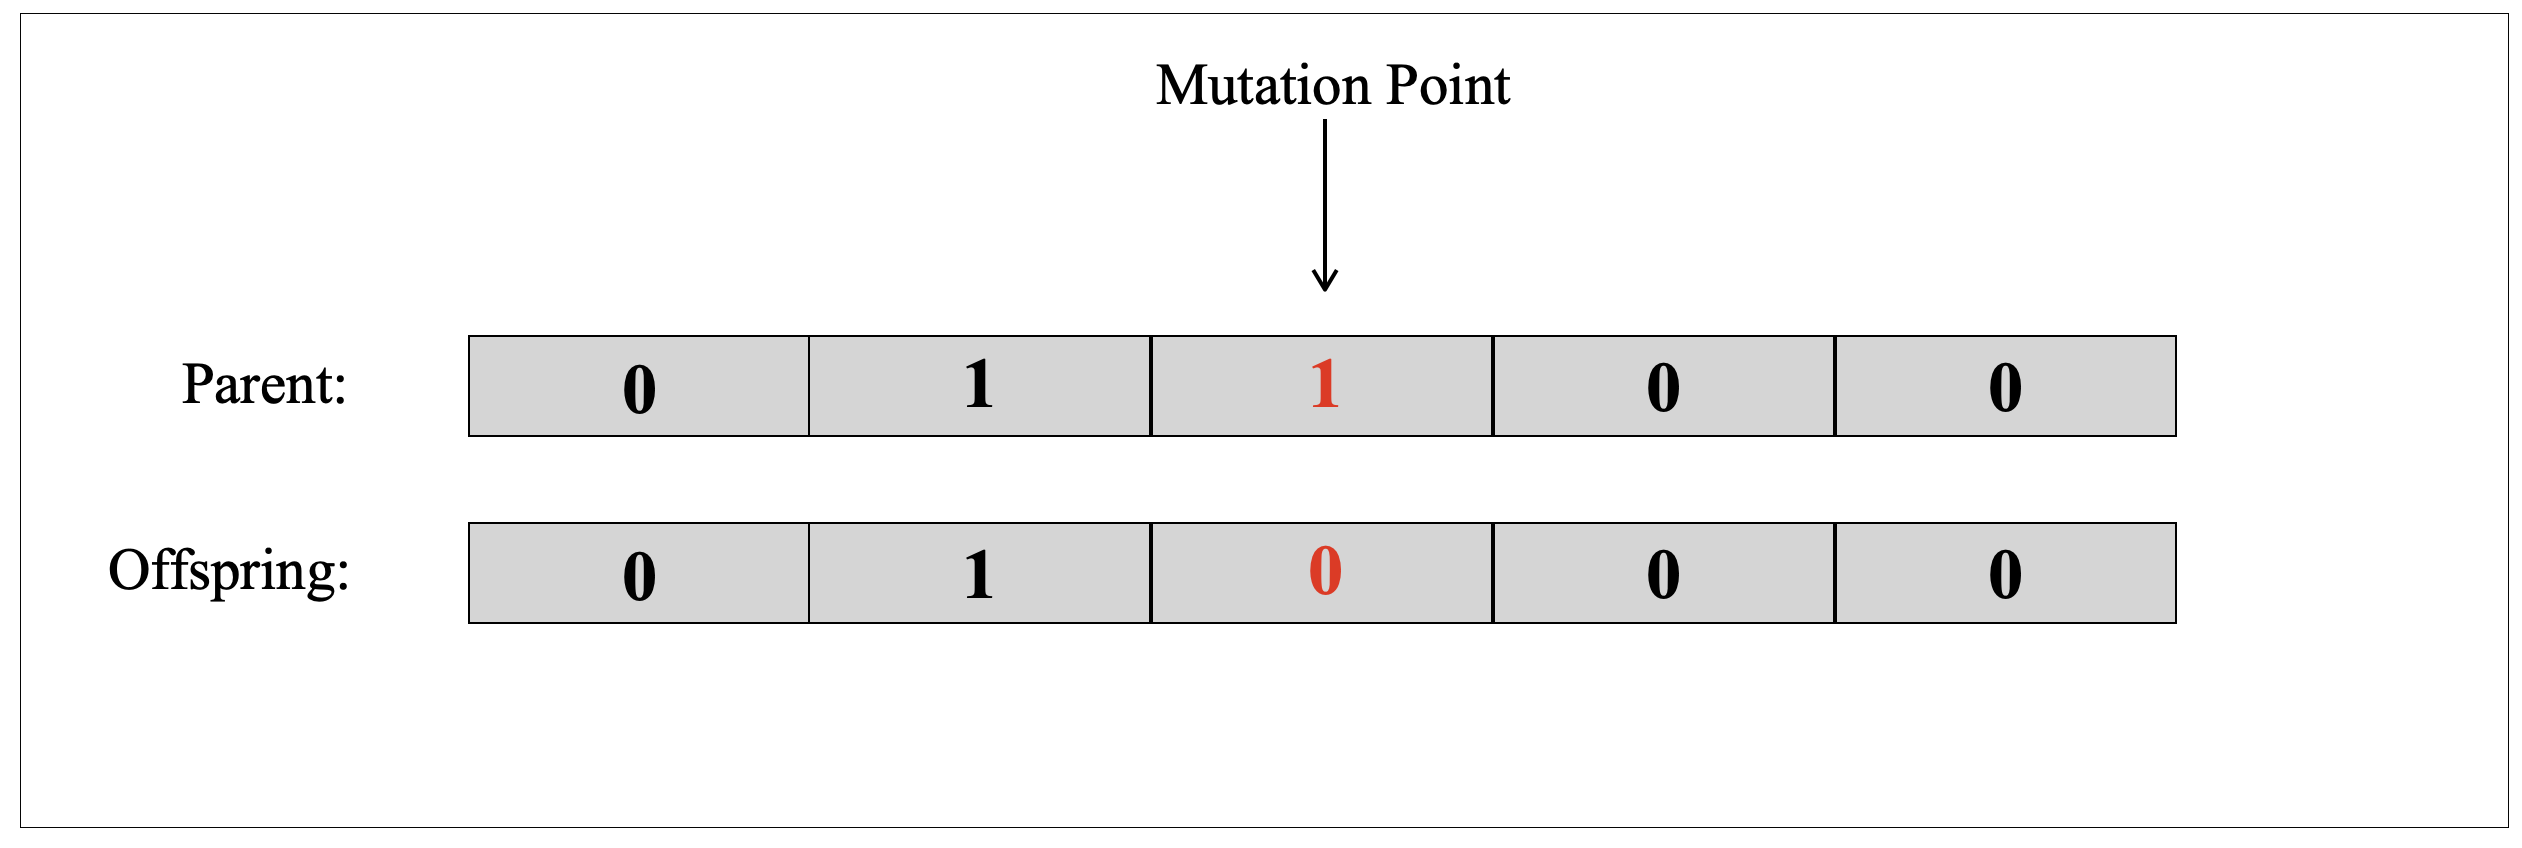
\includegraphics[width=\textwidth]{literature_review/bitwise_mutation_example.png}
    \caption{Example of a bitwise mutation}
    \label{fig:bitwise_mutation}
\end{figure}
\begin{figure}[ht]
    \centering
    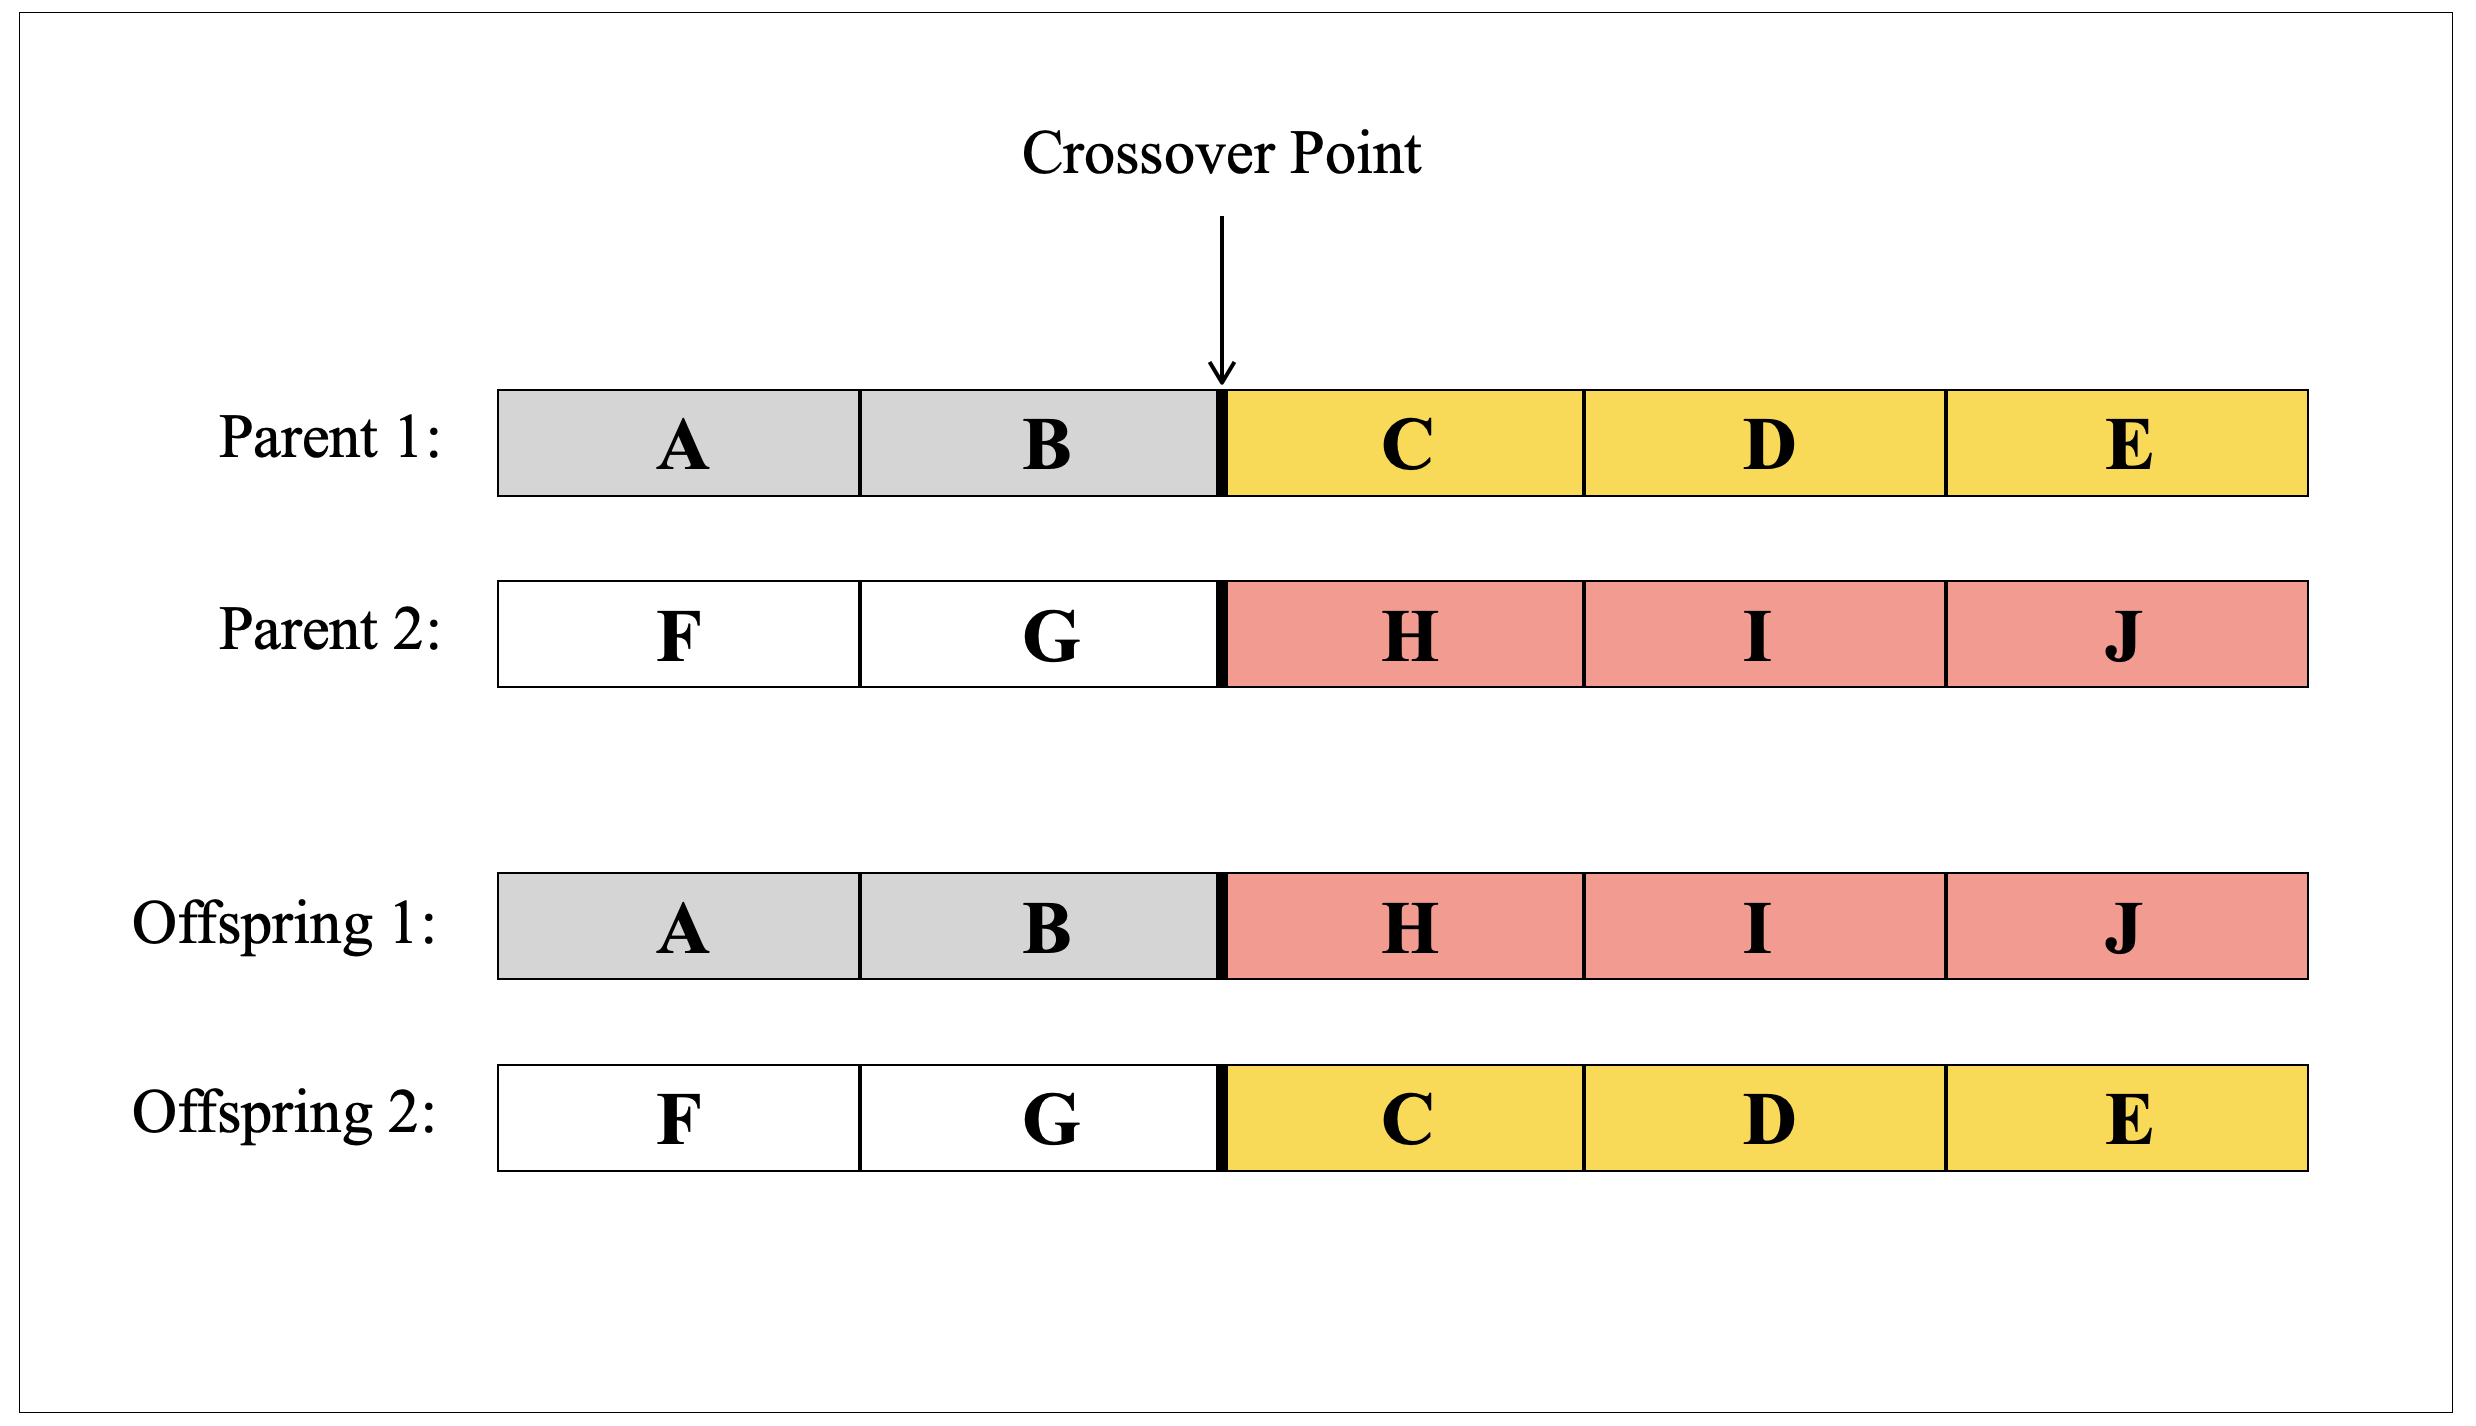
\includegraphics[width=\textwidth]{literature_review/single_point_crossover_example.png}
    \caption{Example of a single-point crossover}
    \label{fig:single_point_crossover}
\end{figure}
\begin{figure}[ht]
    \centering
    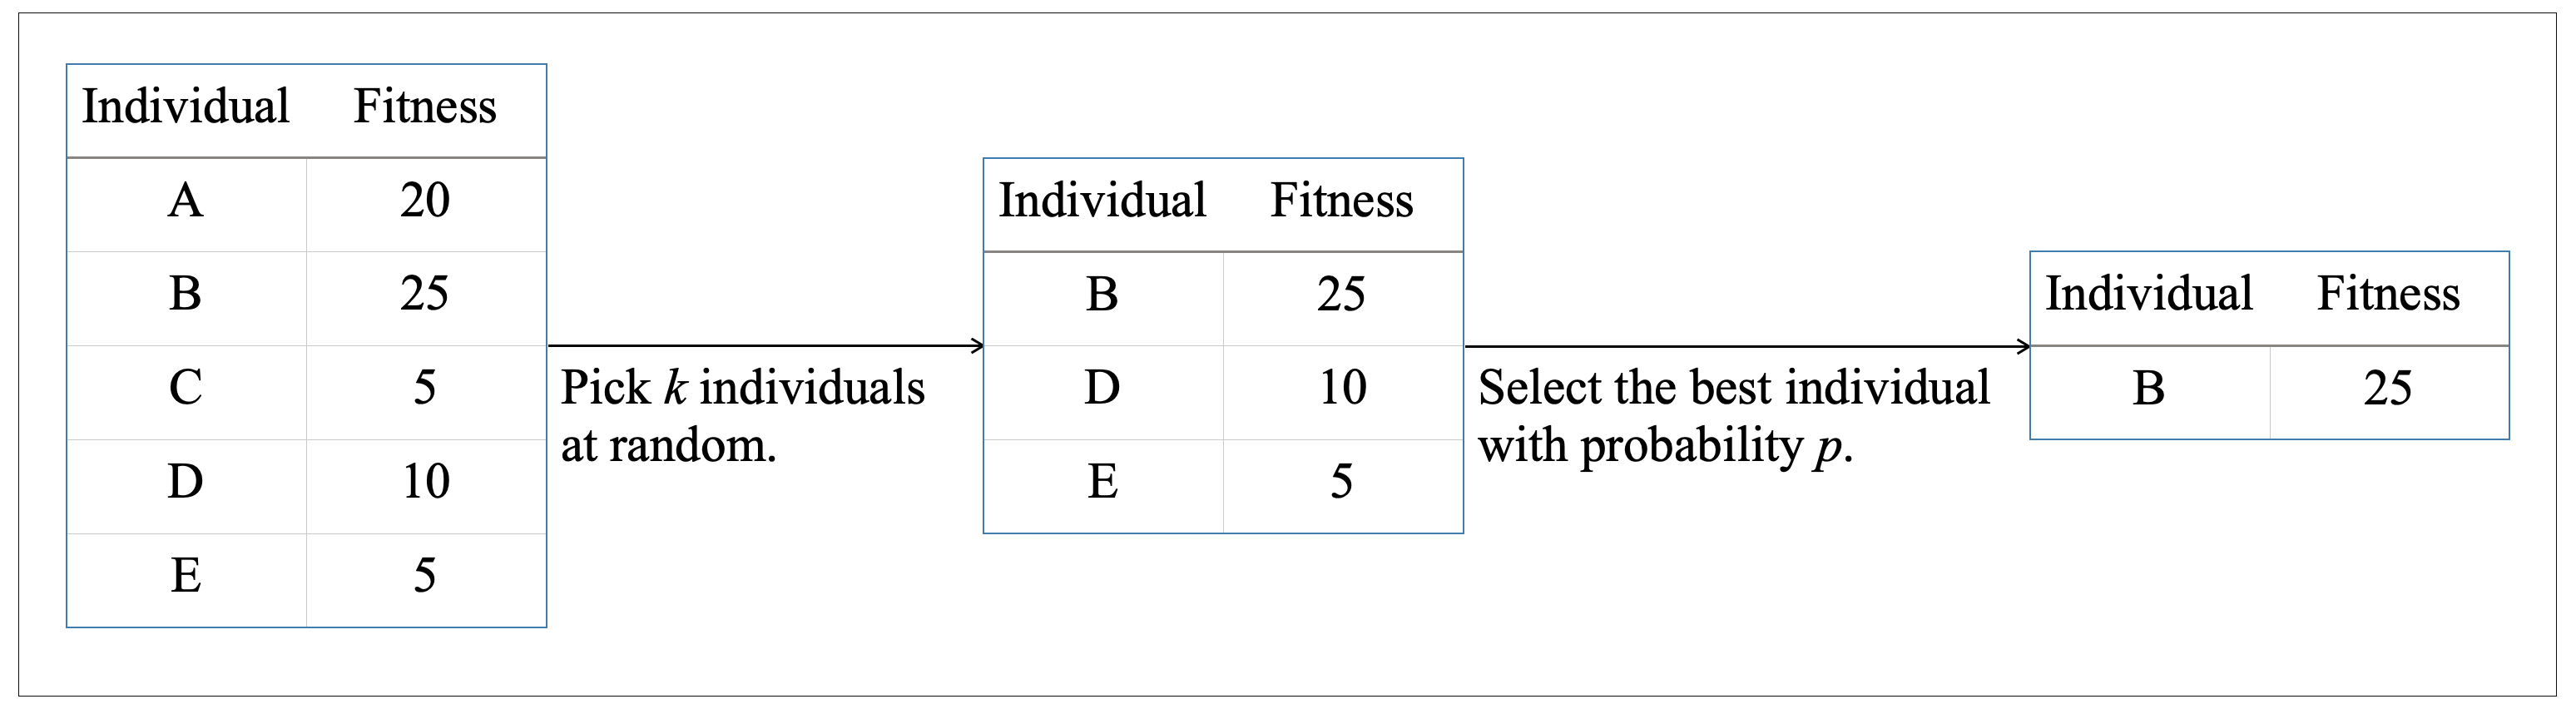
\includegraphics[width=\textwidth]{literature_review/tournament_selection_example.png}
    \caption{Example of the tournament selection procedure}
    \label{fig:tournament_selection}
\end{figure}
\clearpage
\section{Conclusion}
We started this chapter by providing the motivation of this Thesis, looking at different types of present statistics for the topic of recycling. We then gave some background knowledge and definitions of linear and mixed-integer linear programming. Moreover, we introduced single and multi-objective problems. We also introduced the Pareto terminology needed to understand the subsequent sections, looking into Pareto dominance, optimal set, and front. Finally, to understand the following chapters, we illustrated the basic procedure of an evolutionary algorithm and gave fundamental mutation and crossover operators.

\chapter[Literature Review]{Literature Review}
The following sections aim to inspect the literature and research in the sphere of waste management optimisation, exact solution algorithms, and evolutionary algorithms.
\section{Waste Management Optimisation}\label{sec:wmo}
Researchers have sparingly investigated sustainable waste management optimization. \cite{brandenburg_quantitative_2014} give insight into recent supply chain management (SCM) literature. They write that most papers often choose model types and techniques as multi-criteria decision making (MCDM) and mathematical programming, with very few papers focusing on genetic algorithms, dynamic programming, and neural networks as solution techniques.\\
\\
Furthermore, researchers are investigating the sphere of vehicle routing. A 2019 paper proposes a novel way to find the location of waste sorting centres. It finds the optimal routes using a vehicle routing problem model and tries to find the waste sorting locations while investigating the economic, environmental and social aspects. \cite{farahbakhsh_sustainable_2019}\\
\\

\cite{olapiriyakul_multiobjective_2019} advance the field of sustainable waste management by proposing a multi-objective model to create a cost-effective waste management supply chain to help waste disposal for rapidly urbanising cities and developing countries. It focuses on three primary sustainability issues: environmental, social, and economic. In the context of the environmental issue, the authors specifically consider the land-use stress caused by municipal solid waste management (MSWM) by including a land-use equality objective to obtain a fairly distributed network design across the area. For the economic issue, they consider facility and transportation costs. Furthermore, they introduce a measure for the impact of the MSWM on human health based on the disability-adjusted life years (DALYs) metric, commonly used by the World Health Organization (WHO) as a measure of the global burden of disease.\\
The optimization model considers a 3-echelon supply chain where solid wastes are in collection centres, then moved by a small truck to the sorting facilities, and finally sent by a large truck to either an incinerator or landfill facility. The model can make decisions on the locations and sizes of the facilities in tier 2 and tier 3 of the supply chain (i.e. sorting and landfill/incinerator facilities). The main objective is to determine the locations, sizes, and routes to minimize cost, land use, and the impact on public health. \\
\cite{olapiriyakul_multiobjective_2019} describe the single-objective and multi-objective problems as Mixed Integer Linear Programming (MILP) minimisation problems.
\\
\\
\textit{Sets and Indices}
\begin{enumerate}[label=\alph*)]
\item $I$ is the set of collection centers, indexed by $i$;
\item $J$ is the set of sorting facility locations, indexed by $j$;
\item $K$ is the set of incinerator facility locations, indexed by $k$;
\item $K'$ is the set of landfill facility locations, indexed by $k'$;
\item $L(j)$, $L(k)$, and $L(k')$ are the set of available sizes at locations $j$, $k$, and $k'$, indexed by $l$.
\end{enumerate}
\textit{Parameters}
\begin{enumerate}[label=\alph*)]
\item $t_{ij}$, $t_{jk}$, and $t_{jk'}$ are the transportation costs on links ($i$, $j$), ($j$, $k$), and ($j$, $k'$), respectively;
\item $c_{jl}$, $c_{kl}$, and $c_{k'l}$ are the fixed costs to open facilities of size $l$;
\item $C_{jl}$, $C_{kl}$, and $C_{k'l}$ are the storage capacities of facilities of size $l$;
\item $\overline{C}_{ij}$, $\overline{C}_{jk}$, and $\overline{C}_{jk'}$ define the maximum amount of waste a single trip can carry over links ($i$,$j$), ($j$,$k$), and ($j$,$k'$), respectively;
\item $o_j$, $o_k$, and $o_{k'}$ are unit operation costs to manage the flow of solid waste, for each facility;
\item $s_{jl}$, $s_{kl}$, $s_{k'l}$ are land-use stress ratios for facilities of size $l$;
\item $D_i$ is the amount of solid waste available at collection center $i$;
\item $p_{ij}$, $p_{jk}$, and $p_{jk'}$ are the number of people living nearby links ($i$, $j$), ($j$, $k$), and ($j$, $k'$), respectively;
\item $p_{jl}$, $p_{kl}$, and $p_{k'l}$ are the number of people living near a facility of size $l$;
\item $d_{ij}$, $d_{jk}$, and $d_{jk'}$ are the DALYs per person due to transportation activities on links ($i$, $j$), ($j$, $k$), and ($j$, $k'$), respectively;
\item $d_{jl}$, $d_{kl}$, and $d_{k'l}$ are the DALYs per person due to size $l$ facility operations.
\end{enumerate}
\textit{Decision Variables}
\begin{enumerate}[label=\alph*)]
\item $y_{jl}$, $y_{kl}$, and $y_{k'l}$ are binary facility location variables equal to $1$ when sorting, incinerator, and landfill facilities of size $l$ are open at their respective locations, $j$, $k$, and $k'$;
\item $x_{ij}$, $x_{jk}$, and $x_{jk'}$ are the number of vehicle trips on links ($i$, $j$), ($j$, $k$), and ($j$, $k'$), respectively;
\item $f_{ij}$, $f_{jk}$, and $f_{jk'}$ indicates the amount of solid waste transported on links ($i$, $j$), ($j$, $k$), and ($j$, $k'$), respectively.
\end{enumerate}
\textit{Objective Functions}
\\
The MILP model comprises three objective functions: the cost objective function $F_c$, the land-usage objective function $F_u$, and the health-impact objective function $F_h$.
\begin{equation}\label{Fc}
    \begin{aligned}
        F_c &= \sum_{j \in \: J} \sum_{l \in L(j)} c_{jl} y_{jl} + \sum_{k \in K} \sum_{l \in L(k)} c_{kl} y_{kl} + \sum_{k' \in K'} \sum_{l \in L(k')} c_{k'l} y_{k'l} 
        \\ &+ \sum_{i \in I} \sum_{j \in \: J} (t_{ij} + o_{j}) x_{ij} + \sum_{j \in \: J} \sum_{k \in K} (t_{jk} + o_{k}) x_{jk} \\ &+ \sum_{j \in \: J} \sum_{k' \in K'} (t_{jk'} + o_{k'}) x_{jk'}
    \end{aligned}
\end{equation}
The cost objective, $F_c$, comprises fixed costs to open sorting, incinerator, and landfill facilities and the operational cost of transporting and managing solid waste flow throughout the network.
\begin{equation}\label{Fu}
    \begin{aligned}
        F_u &= \sum_{j \in \: J} \sum_{l \in L(j)} s_{jl} y_{jl} + \sum_{k \in K} \sum_{l \in L(k)} s_{kl} y_{kl} + \sum_{k' \in K'} \sum_{l \in L(k')} s_{k'l} y_{k'l} 
    \end{aligned}
\end{equation}
The land-usage objective, $F_u$, is the sum of all land-use ratios throughout the network. The parameters $s_{jl}$, $s_{kl}$, and $s_{k'l}$ denote the total land used and available land ratios.
\cite[~p.~7]{olapiriyakul_multiobjective_2019} use the following ratio to compute the parameters $s_{jl}$, $s_{kl}$, and $s_{k'l}$.
\begin{equation}\label{ratio}
    \frac{\text{Direct + Indirect land use, with a facility of size } l}{\text{Total land available}}
\end{equation}
The third objective function is the health-impact objective, $F_h$, which evaluates the impact of transportation and facilities on the population.
\begin{equation}\label{Fh}
    \begin{aligned}
        F_h &= \sum_{j \in \: J} \sum_{l \in L(j)} p_{jl} d_{jl} y_{jl} + \sum_{k \in K} \sum_{l \in L(k)} p_{kl} d_{kl} y_{kl} + \sum_{k' \in K'} \sum_{l \in L(k')} p_{k'l} d_{k'l} y_{k'l} 
        \\ &+ \sum_{i \in I} \sum_{j \in \: J} p_{ij} d_{ij} x_{ij} + \sum_{j \in \: J} \sum_{k \in K} p_{jk} d_{jk} x_{jk} + \sum_{j \in \: J} \sum_{k' \in K'} p_{jk'} d_{jk'} x_{jk'}
    \end{aligned}
\end{equation}
\textit{Constraints}

\begin{alignat}{4}
& \sum_{j \in \: J} f_{ij}  = D_i, &  \forall i \in I \label{outflow} \\
& \sum_{i \in  I} f_{ij}  = \sum_{k \in K \cup K'} f_{jk}, &  \forall j \in J \label{flow_balance} \\
& \sum_{i \in I} f_{ij} \leq \sum_{l \in L(j)} C_{jl} y_{jl}, &  \forall j \in J \label{size_dependent_j} \\
& \sum_{j \in \: J} f_{jk} \leq \sum_{l \in L(k)} C_{kl} y_{kl}, &  \forall k \in K \label{size_dependent_k} \\
& \sum_{j \in \: J} f_{jk'} \leq \sum_{l \in L(k')} C_{k'l} y_{k'l}, &  \forall k' \in K' \label{size_dependent_k_prime} \\
& f_{ij} \leq \overline{C}_{ij} x_{ij}, &  \forall i \in I, j \in J \label{transportation_capacity_ij} \\
& f_{jk} \leq \overline{C}_{jk} x_{jk}, &  \forall j \in J, k \in K \label{transportation_capacity_jk} \\
& f_{jk'} \leq \overline{C}_{jk'} x_{jk'}, &  \forall j \in J, k' \in K' \label{transportation_capacity_jk_prime} \\
& \sum_{l \in L(j)} y_{jl} \leq 1, &  \forall j \in J \label{one_size_j} \\
& \sum_{l \in L(k)} y_{kl} \leq 1, &  \forall k \in K \label{one_size_k} \\
& \sum_{l \in L(k')} y_{k'l} \leq 1, &  \forall k' \in K' \label{one_size_k_prime} \\
& y_{jl}, y_{kl}, y_{k'l} \in \{0,1\}, &  \forall j, k, k', l \label{y_domains} \\
& x_{ij}, x_{jk}, x_{jk'} \in \mathbb{Z}^{+}, &   \forall i, j, k, k' \label{x_domains} \\
& f_{ij}, f_{jk}, f_{jk'} \geq 0, &  \forall i, j, k, k' \label{f_domains}
\end{alignat}

Equation (\ref{outflow}) declares that the outflow of waste from any collection centre $i$ must be equal to the demand $D_i$. Constraint (\ref{flow_balance}) is a flow balance restriction, which enforces that the inflow at any sorting facility $j$ is forwarded to the incinerators $k$ and landfills $k'$. Constraints (\ref{size_dependent_j}) - (\ref{size_dependent_k_prime}) are capacity constraints for all network facilities. These enforce that the flow into a facility is at most equal to the facility's capacity. The inequalities (\ref{transportation_capacity_ij}) - (\ref{transportation_capacity_jk_prime}) constrain the vehicle transportation capacity for every link ($i$, $j$), ($j$, $k$), and ($j$, $k'$), respectively. Constraints (\ref{one_size_j}) - (\ref{one_size_k_prime}) enforce that each open facility can have at most one facility size selected. Finally, equations (\ref{y_domains}) - (\ref{f_domains}) define the decision variables' domains, where (\ref{y_domains}) are binary values, (\ref{x_domains}) are positive integer values, and (\ref{f_domains}) are real numbers that are at least 0.
\newline \newline 
To allow for a multi-objective MILP optimisation, \cite[pp.~5 --- 6]{olapiriyakul_multiobjective_2019}  use a min-max approach which minimises the deviations from the ideal results.
The deviations use the optimal values $F^{*}_{c}$, $F^{*}_{u}$, and $F^{*}_{h}$, obtained by solving their respective single-objective problem. Moreover, $F^{max}_{c}$, $F^{max}_{u}$, and $F^{max}_{h}$ are the upper bounds obtained by the worst values for each function across the single-objective problems. Normalisation according to the ideal target occurs for each function to compute the deviation values.
\begin{alignat}{2}
    \sigma_c & = \frac{F_c - F^*_c}{F^{max}_c - F^*_c} \label{deviation_cost}\\
    \sigma_u & = \frac{F_u - F^*_u}{F^{max}_u - F^*_u} \label{deviation_land} \\
    \sigma_h & = \frac{F_h - F^*_h}{F^{max}_h - F^*_h} \label{deviation_health}
\end{alignat}
\cite{olapiriyakul_multiobjective_2019} add a new continuous variable, $z$, which minimises the deviation levels of the objective functions. The multi-objective formulation of the problem is thus a min-max on the deviations of the objective functions as follows.
\begin{alignat}{2}
    \text{min} \enspace & z \\
    \text{s.t.} \enspace & \sigma_c \leq z \\
    & \sigma_u \leq z \\
    & \sigma_h \leq z \\
    & (\ref{outflow}) \: \text{--} \: (\ref{f_domains})
\end{alignat}
\clearpage
\section{Exact Solution Algorithms}
This section overviews the exact algorithmic approaches in the literature to solving MILP and combinatorial optimisation problems.
\subsection{Branch and Bound}
\cite{land_automatic_1960} pioneered the famous Branch and Bound algorithm, a search strategy based on a binary enumeration tree. The algorithm consists of two primary operations: \emph{branching} that recursively splits the search space S into smaller spaces, then minimising the objective function $f(x)$, and \emph{bounding}, which attempts to prune the search space, thus eliminating candidate solutions that do not contain an optimal solution.
\begin{definition}[Branch and Bound Operations]
Let $I$ be an instance of a problem, and the set of candidate solutions of an instance $I$ be $S_I$. Then the two operations to the branch and bound algorithm are:
\begin{enumerate}[label=\alph*)]
    \item $branch(I)$, which produces two or more disjoint subsets of $S_I$;
    \item $bound(I)$, which computes the lower bound on the value of candidate solutions in I. $bound(I) \leq f(x), \enspace \forall x \in S_I$.
\end{enumerate}  
\qed
\end{definition}

\begin{algorithm}
\caption{Generic Branch and Bound}\label{alg:b_and_b}
\SetKwInOut{Input}{Input}
\SetKwInOut{Output}{Output}
\Input{A problem $\mathbf{p}$, a objective function $\mathbf{f}$, and a lower bounding function $\mathbf{LB}$.}
\Output{The optimal solution $\mathbf{x^*}$.}
$UB \gets \infty$;\\
$x^* \gets \emptyset$;\\
Initialise a candidate queue based on the problem $Q \gets Q(p)$;\\
\While{$Q \neq \emptyset$}{
   Node $\gets Q$.pop();\\
   \eIf{Node $N$ represents a single candidate solution $x$ \textit{and} $f(x) < B$}{
        $x^* \gets x$;\\
        $UB \gets f(x^*);$
   }{\ForEach{child $N_i \in \text{Node} \: N$}{
        \If{$LB(N_i) \leq UB$}{
            $Q \gets Q.enqueue(N_i)$;}
        }
   }
}
\end{algorithm}
\subsection{Branch and Cut}
To extend the branch and bound algorithm to integer linear problems (ILPs) or MILPs, a method known as branch and cut combines the branch and bound algorithm with cutting planes. \cite{gomory_algorithm_1960} proposed the \emph{cutting plane method}, which includes a \emph{cut} as an inequality constraint that tightens a relaxed problem's solution space without cutting out any candidate solution in $S$.  Cutting planes can find an optimal solution to ILPs in a finite number of iterations. However, it is ineffective as many rounds of cuts are needed to progress towards a solution. For this reason, the generation of cuts is combined with branch and bound, resulting in the \emph{branch and cut} approach.\\
We can relax an integer linear program by removing the integrality constraint of each variable. For example, if we take a binary integer program, then all the constraints are of the form:
\begin{equation}
    x_i \in \{0,1\}.
\end{equation}
The relaxed form of the problem converts these constraints into linear constraints:
\begin{equation}
    0 \leq x_i \leq 1.
\end{equation}
This relaxation helps to find a bound on an integer program's solution. Coupled with branch and bound, this provides an exact solution to complex optimisation problems. Algorithm \ref{alg:b_and_c} shows the pseudocode for the branch and cut algorithm for a minimisation problem.
\begin{algorithm}
\caption{Generic Branch and Cut}\label{alg:b_and_c}
\SetKwInOut{Input}{Input}
\SetKwInOut{Output}{Output}
\Input{An integer linear programming problem $\mathbf{p}$, an objective function $\mathbf{f}$.}
\Output{The optimal solution $\mathbf{x^*}$.}
Add the initial problem to a queue $Q$:\\
$Q \gets Q.enqueue(p)$;\\
$v^* \gets \infty$;\\
$x^* \gets \emptyset$;\\
\While{$Q \neq \emptyset$}{
   \emph{Obtain a problem from the queue $Q$:}\\
   $P \gets Q.dequeue(Q);$\\
   \emph{Solve the linear programming relaxation of $P$:}\\
   $R \gets relax(P)$;\\
   $x \gets solve_LP(R)$;\\
   \If{$\neg x.isfeasible()$ \textbf{or} $v^* \geq f(x)$}{
        Go back to step $5$.
   }
   \If{$x.isinteger()$}{
        $x^* \gets x$;\\
        $v^* \gets f(x)$;\\
        Go back to step $5$.
   }
   \emph{Search for violated cutting planes:}\\
   $VCP  \gets$ ViolatedCuttingPlanes($x$)\\
   \If{$VCP \neq \emptyset$}{
   \ForEach{Cutting plane $CP \in VCP$}{
        $Q \gets Q.enqueue(relax(P), CP)$;
   }
   Go back to step $8$.
   }
   \emph{Branch to partition the problem into new problems:}\\
   $N \gets branch(P)$;\\
   \ForEach{child $N_i \in$ Branch $N$}{
        $Q \gets Q.enqueue(N_i)$;
   }
}
\Return{$x^*$}
\end{algorithm}
\clearpage
\section{Heuristic Solution Algorithms}
This section overviews the heuristic algorithmic approaches in the literature to solving MILPs and multi-objective combinatorial optimisation problems.
\subsection{Multi-objective optimisation with NSGA}
NSGA (Non-dominated Sorting Genetic Algorithm) is one example of a famous multi-objective evolutionary algorithm. It uses dominance ranking to move the population to the Pareto front in a multi-objective problem. To determine the dominance rank of an individual, we count how many individuals are dominating this individual. The result of a dominance ranking procedure, as shown in fig. \ref{fig:dominance_ranking}, is a partially ordered list used for sorting the points before utilising the selection operator. \cite[~pp.~79--81]{coello_coello_basic_2007}

In addition, it also uses a technique named fitness sharing (or niching), seen in fig. \ref{fig:fitness_sharing}, where one counts how many solutions are in a neighbourhood of solutions and proportionally decreases the fitness of the solutions in the same neighbourhood. It introduces a neighbourhood radius, $\sigma_{share}$, to control the size of a neighbourhood. Fitness sharing promotes the creation of solutions in the least populated regions of the search space. \cite[~p.~81]{coello_coello_basic_2007} 
\begin{figure}[ht]
    \centering
    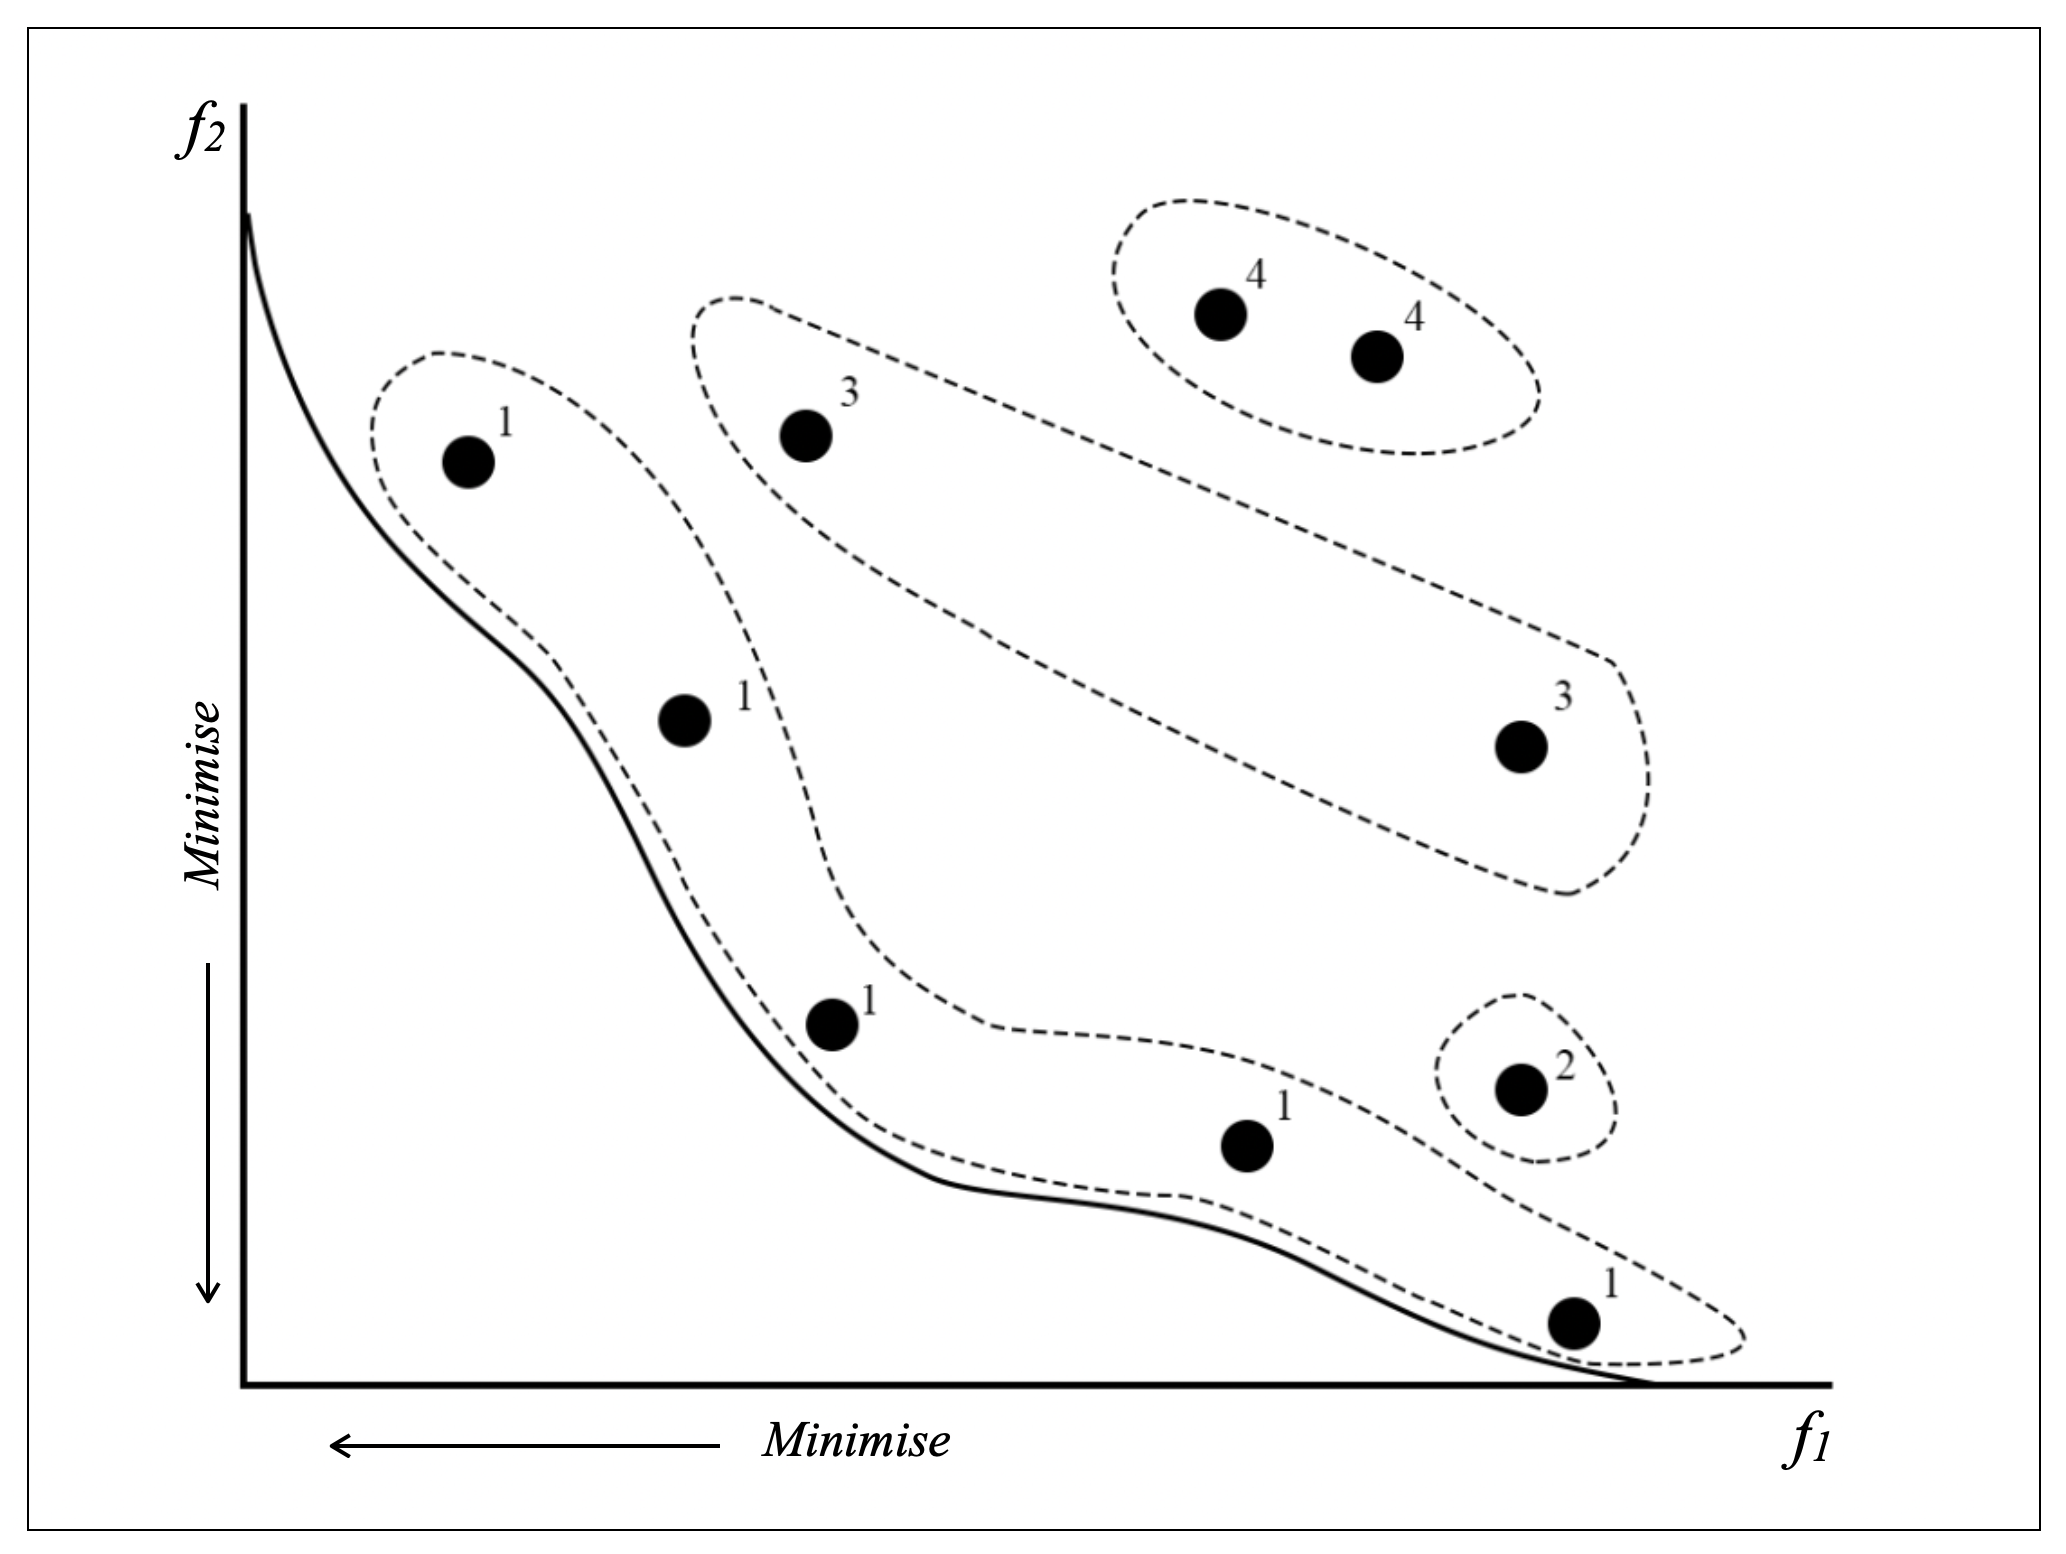
\includegraphics[scale=0.32]{literature_review/dominance_ranking.png}
    \caption{Dominance ranking example with the grouping of equal ranks for sorting. (Adapted from \cite[~p.~80]{coello_coello_basic_2007})}
    \label{fig:dominance_ranking}
\end{figure}
\begin{figure}[ht]
    \centering
    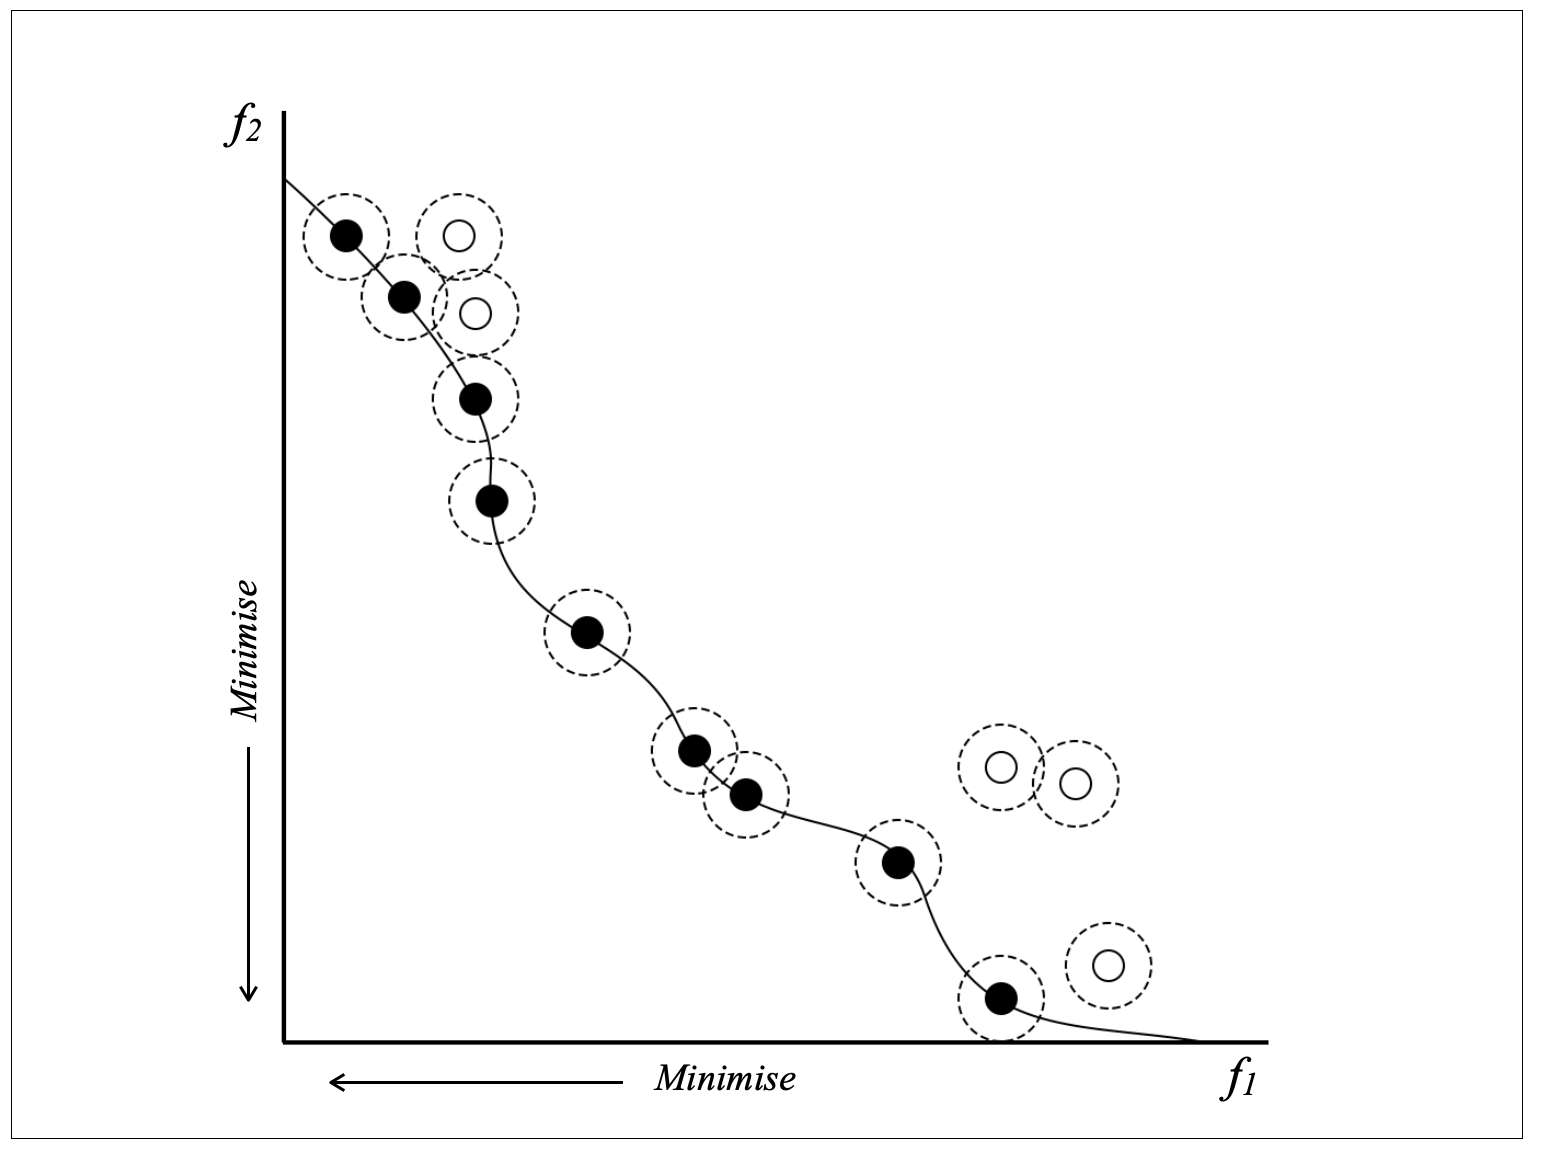
\includegraphics[scale=0.43]{literature_review/fitness_sharing.png}
    \caption{An illustration of the fitness sharing scheme. (Adapted from \cite[~p.~82]{coello_coello_basic_2007})}
    \label{fig:fitness_sharing}
\end{figure}

NSGA uses these techniques in conjunction with the population being ranked based on dominance and classified into a hierarchy of subpopulations based on the order of domination. 
\\\\
NSGA then evaluates the similarity between the members of these subgroups using the fitness sharing approach to promote population diversity. An advantage of this approach is that the individuals in the first front obtain more copies than the rest of the population due to their higher fitness values, which allows for a convergence of the population towards the known Pareto front regions. \cite[~pp.~91--93]{coello_coello_basic_2007}
\\\\
Nonetheless, a disadvantage of NSGA is that it uses the fitness sharing mechanism. \cite{deb_fast_2002} write that there are two issues with the sharing approach.
\begin{enumerate}
    \item ``The performance of the sharing function method in maintaining a spread of solutions depends largely on the chosen $\sigma_{share}$ value.'' \cite[~p.~184]{deb_fast_2002}
    \item ``Since each solution must be compared with all other solutions in the population, the overall complexity of the sharing function approach is $\mathcal{O}(N^2)$.'' \cite[~p.~185]{deb_fast_2002}
\end{enumerate}

\subsubsection{NSGA-II}\label{sec:nsga2}
NSGA-II addresses this bottleneck by using a crowding sort technique using the crowding distance. The crowding distance measures the density of solutions surrounding a particular solution in the population. In fig. \ref{fig:crowding_distance}, we can see an illustration of the crowding distance. To calculate the crowding distance of a particular solution, $i$, the following equation is applied, where $f^{max}_k$ and $f^{min}_k$ are the maximum and minimum values of the $k$th objective function.
\begin{equation}
    D_i = \sum_{k \in K} \frac{f_{k}(i + 1) - f_{k}(i - 1)}{f^{max}_{k} - f^{min}_{k}}
\end{equation}
NSGA-II uses crowding distance sorting, where sorting occurs on the population in ascending order of magnitude before calculating the crowding distance. According to \cite[~p.~185]{deb_fast_2002}, this approach's algorithmic complexity is $\mathcal{O}(MN \log N)$, with M independent sortings of at most N solutions.
\begin{figure}[ht]
    \centering
    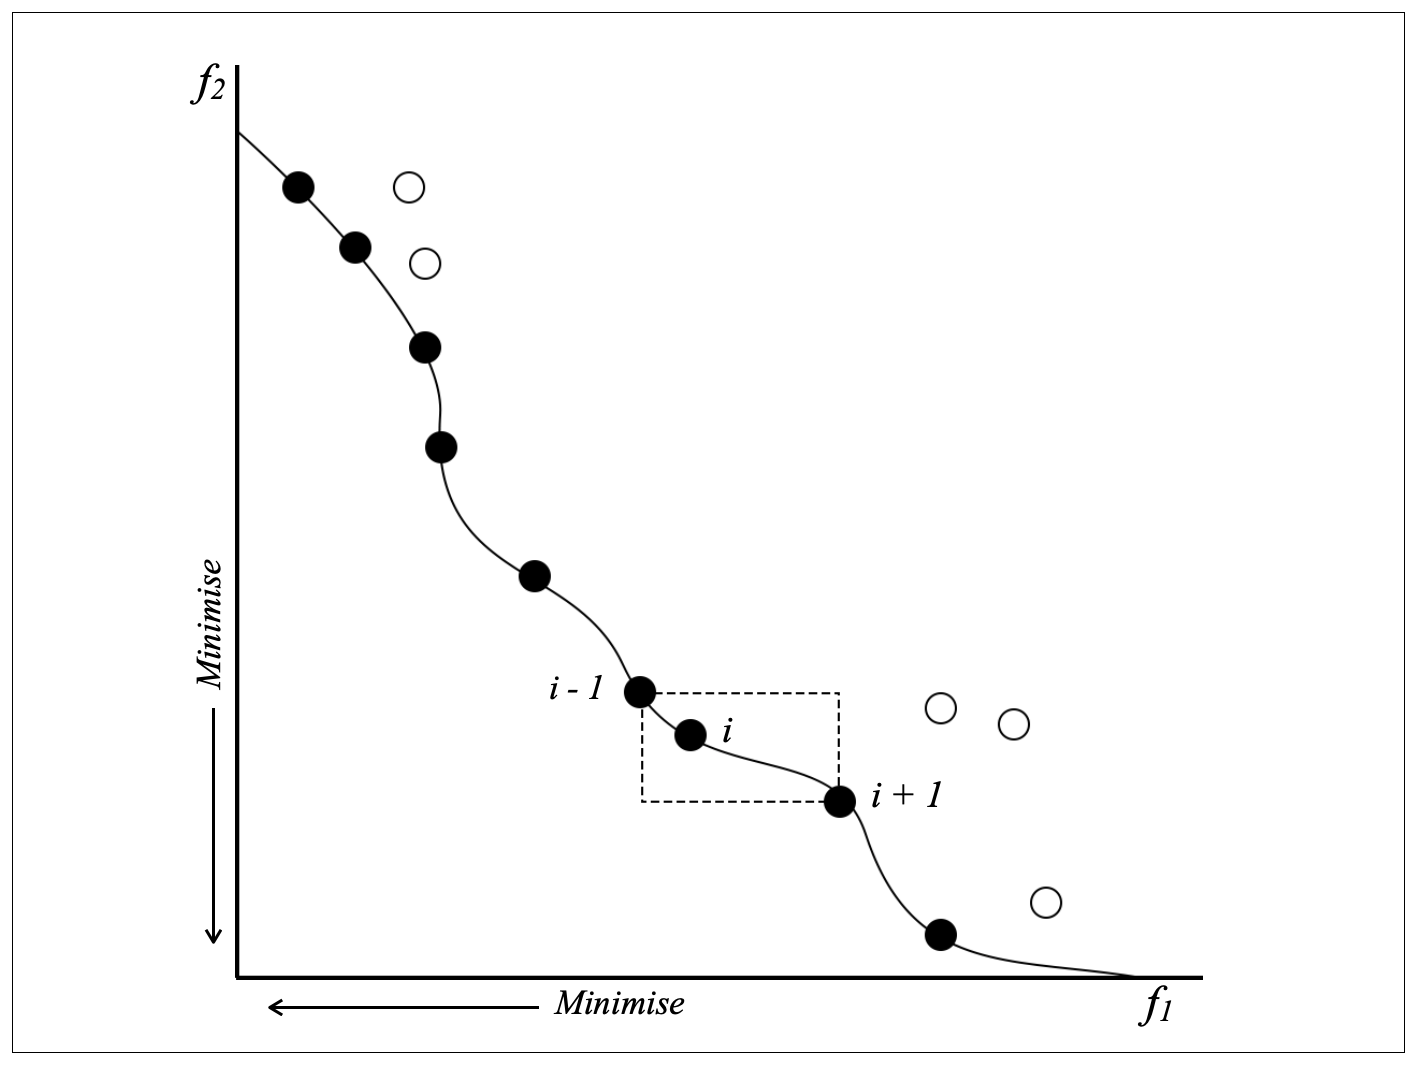
\includegraphics[scale = 0.45]{literature_review/crowding_distance.png}
    \caption{Illustration of the crowding distance. (Adapted from \cite[~p.~83]{coello_coello_basic_2007})}
    \label{fig:crowding_distance}
\end{figure}
\begin{figure}[ht]
    \centering
    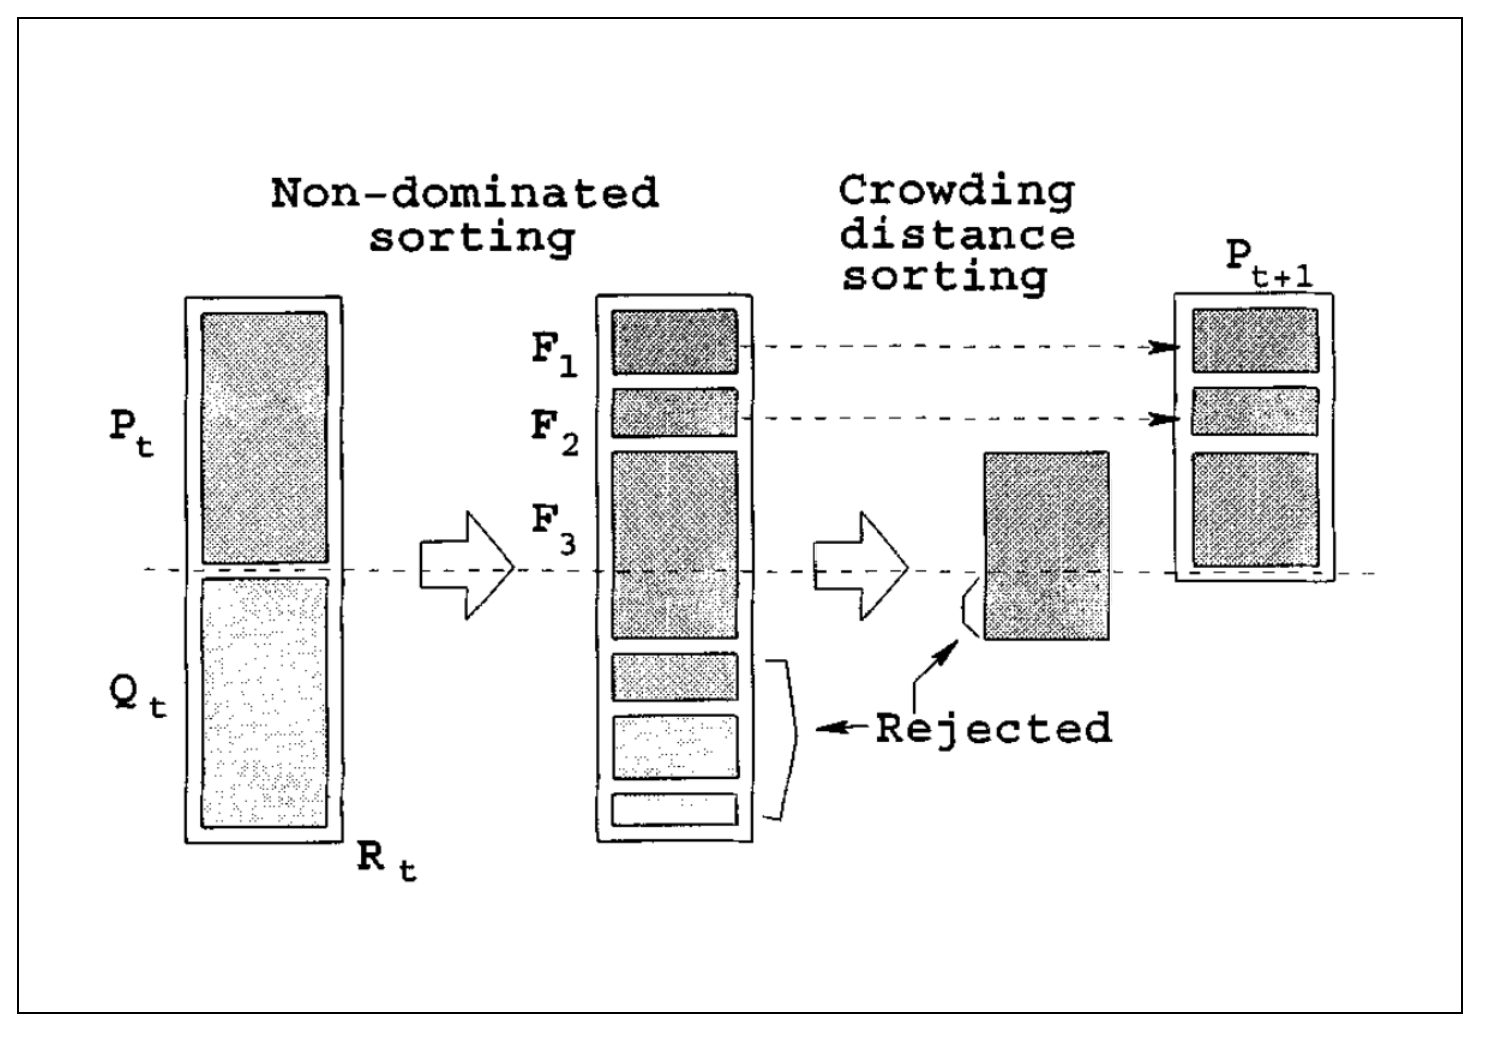
\includegraphics[scale = 0.4]{literature_review/nsga2_procedure.png}
    \caption{The procedure of NSGA-II. \cite[~p. 186]{deb_fast_2002}}
    \label{fig:nsga2_procedure}
\end{figure}

In fig. \ref{fig:nsga2_procedure}, NSGA-II builds a population of individuals and ranks and sorts each individual according to the non-domination level. It then uses the evolutionary operators to create new offspring. Afterwards, it applies fitness sharing by adding a crowding distance to every individual of the population, which is more efficient than computing the fitness sharing count. 
\\
Crowding distance sorting decides which individuals get added to the new population to keep a diverse front of solutions in the population and avoid local minimums (or maximums). The individuals with higher crowding distances are selected first and filled until it reaches the desired number of parents. The individuals who did not make it into the parent population get rejected.
The algorithmic complexity of NSGA-II, considering the non-dominated sorting, the crowding-distance assignment, and the crowding-distance sorting, is $\mathcal{O}(MN^2)$ \cite[~p.~186]{deb_fast_2002}.
Algorithm \ref{alg:nsga2} illustrates the NSGA-II algorithm from an adaptation of the pseudocode from \cite[~p.~93]{coello_coello_basic_2007} and \cite[~p.~186]{deb_fast_2002}.
\begin{algorithm}[ht]
  \caption{NSGA-II Algorithm}\label{alg:nsga2}
  \SetKwInOut{Input}{Input}
  \Input{Population size $N$, Total generations $g$.}
  Initialise population $P$ with $N$ number of random individuals;\\
  \For{$t = 1$ to $g$}{
  Combine parent and offspring population:\\
  \qquad $R_t \gets P_t \cup Q_t$;\\
  $F \gets$ Apply the non-dominated sorting procedure on $R_t$\\
  $P_{t+1} \gets \emptyset$;\\
  $j \gets 1$;\\
  \While{$|P_{t+1}| + |F_j| \leq N$}{
    Calculate the crowding distance of $F_j$\\
    Include the $j$th non-dominated front into the parent population $P_{t+1}$:\\
    \qquad $P_{t+1} \gets P_{t+1} \cup F_j$;\\
    $j \gets j + 1$;
  }
  Sort $F_j$ in descending order\\
  Add the first $(N - |P_{t+1}|)$ elements of $F_j$ to $P_{t+1}$:\\
    \qquad $P_{t+1} \gets P_{t+1} \cup F_j [1 : (N - |P_{t+1}|)]$;\\
  Create next generation $Q_{t+1}$:\\
  \qquad Binary tournament selection\\
  \qquad Crossover and Mutation\\
  }
\end{algorithm}
\clearpage
\subsection{Generating well-spaced reference points on a unit simplex}\label{ref_points}
Most evolutionary many-objective optimisation (EMaO) algorithms start with a predefined set of reference points on a unit simplex. These points operate as guides to search for a single Pareto optimal solution across each reference direction. The approach by \cite{das_normal-boundary_1998} is the most common method of creating a set of uniformly spaced reference points on a normalised hyperplane. This approach starts by initialising a set of points on a K-dimensional unit simplex to generate reference points subject to,
\begin{equation}
    \sum_{i=1}^K z_i = 1, \quad \text{for} \enspace \mathbf{z} \in [0, 1]^K
\end{equation}

Subsequently, the construction of reference directions uses a vector which originates from the origin and connects to all initialised reference points. The output of this procedure is a K-dimensional unit simplex to all objective axes with an intercept of one on each axis. 
If an EMaO algorithm works well enough to find a single Pareto-optimal solution for one reference direction, then a well-spaced set of Pareto-optimal solutions is anticipated due to the unit simplex. 

The parameter $\rho$, which indicates the number of gaps between two successive points along an objective axis, controls the number of points on the unit simplex. The total number of points, $H$, on a unit simplex are:
\begin{equation}\label{eq:total_simplex_points}
    H = C_{\rho}^{K + \rho - 1}
\end{equation}
Eq. \ref{eq:total_simplex_points} shows a binomial coefficient for the number of points, represented in factorial notation as,
\begin{equation}
    H = \frac{(K + \rho - 1)!}{\rho ! \: (K - 1) !}
\end{equation}
\\
A problem arises with this approach when there are a preferred number of points. This problem occurs as there is a drastic increase in the number of points when increasing p by one. Another problem with the \cite{das_normal-boundary_1998} approach occurs as K increases, the number of total points on the unit simplex increases severely. Moreover, this requires a vast population for the EMaO algorithms as the population size is usually the same as the number of points. 
\\\\
\cite{blank_generating_2021} develop an approach to generating well-spaced points on a unit simplex that mends the abovementioned problems. They introduce a novel method that uses a generalisation of potential energy called \emph{Riesz s-Energy}. 
\begin{definition}[Riesz s-Energy \cite{hardin_minimal_2005}]
    Let $\mathbf{x} = \{x_1, ..., x_N\}$ denote a set of $N$ distinct points in the $d$-dimensional unit sphere $S^d \in \mathbb{R}^{d+1}$ or a rectifiable $d'$-dimensional manifold embedded in $\mathbb{R}^{d'}$, where $s > 0$ is a fixed parameter, then the definition of the Riesz s-Energy is
    \begin{equation}
        E_s (\mathbf{x}) = \sum_{i = 1}^N \sum_{\substack{j = 1 \\ i \neq j}}^N \frac{1}{\lVert x_i - x_j \rVert^s}
    \end{equation}
    \qed
\end{definition}
\cite[~p.~53]{blank_generating_2021} set $s = K^2$ motivated by trial-and-error studies. The goal of the energy method is to find the $\mathbf{x}$-matrix of size $\mathbb{R}^{N \times K}$ that minimises the total energy $E_s$ subject to $\sum_{k=1}^K x_k = 1$. \cite{blank_generating_2021} use the Adam gradient optimiser to minimise this problem. As $E_s$ has a considerable magnitude, the authors take the logarithm of $E_s$ and then compute the partial derivative of $F_E = \log E_s$ w.r.t $x_k$ as follows.
\begin{equation}
    \frac{\partial F_E}{\partial x_{k}^{(i)}} = - \frac{s}{E_s} \left[\sum_{\substack{j = 1 \\ i \neq j}}^N \frac{x^{(i)}_k - x^{(j)}_k}{\lVert \mathbf{x}^{(i)} - \mathbf{x}^{(j)} \rVert^{s+2}} \right]
\end{equation}
Finally, the authors project the gradients onto the unit simplex to ensure that all points stay on the unit simplex. Figure \ref{fig:riesz_s_energy_91_92} displays the distribution of $91$ circle and $92$ cross points on the unit simplex. The $92$ points are not possible with the method from \cite{das_normal-boundary_1998}. Interestingly, the lower right corner points get readjusted to accommodate the extra $92$nd point. This method effectively finds a distribution of points that are still very well-spaced even though, to our knowledge, no well-spaced distribution of $92$ points exists.
\begin{figure}[ht]
    \centering
    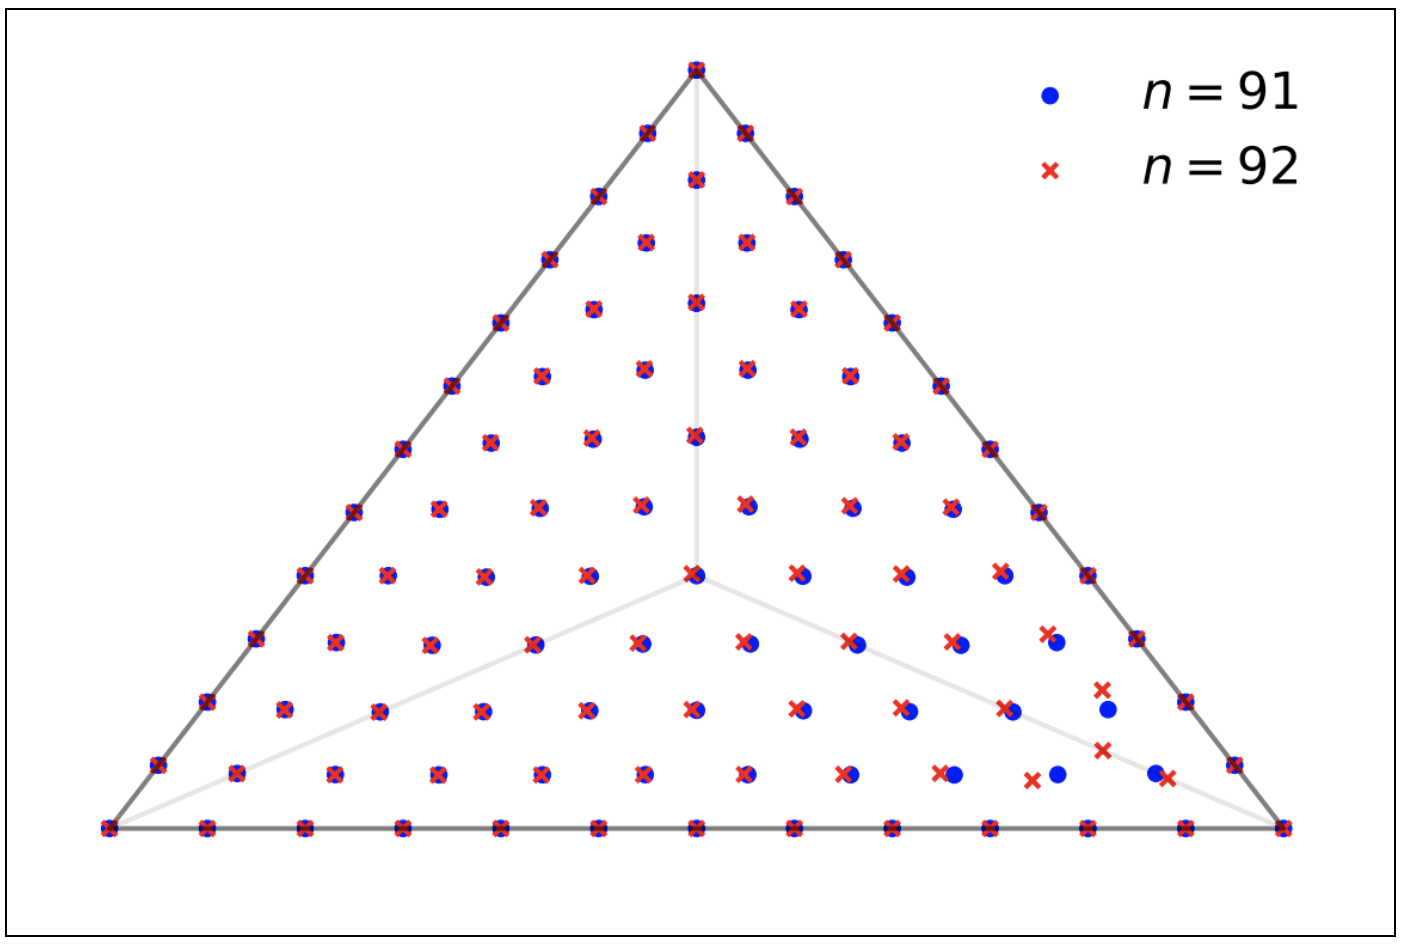
\includegraphics[scale = 0.4]{/literature_review/riesz_s_energy.png}
    \caption{Points obtained by Riesz's s-energy method with 91 circle points and 92 cross points. (Taken from \cite[~p.~57]{blank_generating_2021}}
    \label{fig:riesz_s_energy_91_92}
\end{figure}
\clearpage
\subsection{Many-objective optimisation using NSGA-III}
\subsubsection{NSGA-III}\label{sec:nsga3}
NSGA-II works best on problems requiring two to three objectives and struggles in handling many objectives. NSGA-III is an extension of NSGA-II that can handle three or more objectives. It achieves this by using a predefined set of reference points, ensuring diversity in the solutions obtained. Usually, the reference points are predefined in a structured manner using the approaches found in section \ref{ref_points}. NSGA-III uses the same non-dominated sorting approach found in NSGA and NSGA-II. As outright computing the crowding distance takes too much computational time on problems with many objective functions, the reference points help to find good representative, non-dominated solutions. 
\\
First, NSGA-III creates a new population, $S$, that fills up the underrepresented reference points using the non-dominated sorted solutions.  If the last accepted non-dominated solution, $F_l$, is only partially added to $S$, NSGA-III selects only the solutions that maximise the diversity of the solution's front. It does this by using an alternative to the crowding operator shown in NSGA-II. The outline of the approach from \cite[~pp.~581--583]{deb_evolutionary_2014} is shown in procedure \ref{proc:crowding_nsga3}. In addition, since NSGA-III assigns only one population member to each reference direction, there is no need for selection, as it would allow for competition between different reference directions.
According to \cite[~p.~583]{deb_evolutionary_2014} the algorithmic complexity of NSGA-III through this procedure is still $\mathcal{O}(MN^2)$.
\begin{definition}[Achievement scalarising function]\label{def:asf}
    Let $\mathbf{w} = \{w_1, w_2, ..., w_K\}$, be a non-negative weight vector with $ w_i \in (0, 1], \enspace \text{for} \enspace i = \{1, ...,K\}$, $f(x) = \{f_1 (x), f_2 (x), ...,f_K (x)\}$ a minimisation (or maximisation) multi-objective optimisation problem, and $\mathbf{z}^* = \{z^{*}_1, z^{*}_2, ..., z^{*}_K\}$ the ideal points for each objective function. Then the definition of an achievement scalarising function is,
    \begin{equation}
        ASF(f(x)\: | \: \mathbf{w, z^*}) = \max_{1 \leq i \leq K} \left \{\frac{f_i(x) - z^{*}_i}{w_i}\right \} 
    \end{equation}
    \qed
\end{definition}
\clearpage

\begin{algorithm}[ht]
    \small
    \SetKwBlock{Begin}{Begin}{}
    \caption{Alternative crowding distance operator for NSGA-III}\label{proc:crowding_nsga3}
    \SetKwInOut{Input}{Input}
    \SetKwInOut{Output}{Output}
    \Input{The output of the non-dominated sorting $\mathbf{F}$, the filled non-dominated sorting population $\mathbf{S}$, and the structured reference points $\mathbf{Z^s}$}
    \Output{The new population $\mathbf{P_{t+1}}$.}
    \begin{enumerate}
        \item \emph{Adaptive Normalisation of Population members}\\
        \begin{enumerate}
            \item Compute the ideal point by taking the minimum value for each objective function.
            \begin{equation}
                z_{k}^{ideal} = \min_{\mathbf{s} \in S} f_k (\mathbf{s}), \quad k = \{1,...,K\}
            \end{equation}
            \item Translate all objective values in the population $S$ by subtracting the ideal point from them.
            \begin{equation}
                f'_{k} (\mathbf{s}) = f_{k} (\mathbf{s}) - z_{k}^{ideal}, \quad \forall \mathbf{s} \in S 
            \end{equation}
            \item Compute the extreme points $z^{k,extreme}$ in each objective axis $k = \{1,...,K\}$ by finding the solution, $s \in S$, which minimises the corresponding \emph{achievement scalarising function} defined in definition \ref{def:asf}.
            \begin{equation}
                z^{k, extreme} = f_k(\mathbf{s}): \argmin_{\mathbf{s} \in S} \left\{ASF(f'(\mathbf{s}) \: | \: \mathbf{w, z^{ideal}})\right\}
            \end{equation}
            \item Computation of the intercept, $a_k$, of the $k$th objective, uses the approach shown in fig. \ref{fig:intercepts_nsga3}. In practice, the computation of the intercept, $a_k$, uses Gaussian Elimination. The normalisation on the objective function occurs using the following equation.
            \begin{equation}
                f^{n}_{k} (\mathbf{s}) = \frac{f'_k (\mathbf{s})}{a_k}, \quad \text{for} \enspace k = \{1, ..., K\}
            \end{equation}
        \end{enumerate}
        \item \emph{Association Operation} to associate each population member with a reference point. 
        \begin{enumerate}
            \item By joining reference points with the origin, create a reference line, $\mathbf{u}$, for each reference point, $z \in Z^s$.
            \item Calculate the perpendicular distance of each population member, $\mathbf{s} \in S$, to each reference line, $\mathbf{u} \in Z^s$. 
            \begin{equation}
                d^{\perp}(\mathbf{s}, \mathbf{u}) = \left\lVert \mathbf{s} - \frac{\mathbf{u}^T \mathbf{su}}{\|\mathbf{u}\|_2} \right\rVert_2
            \end{equation}
            \item Associate the population member in $S$ to the reference point with the closest reference line. 
            \begin{equation}
                \pi(\mathbf{s}) = \mathbf{u} : \argmin_{\mathbf{u} \in Z^s} d^{\perp}(\mathbf{s}, \mathbf{u})
            \end{equation}
        \end{enumerate}
        \item \emph{Niche-Preservation Operation} ensures every reference point has at most one population member.
        \begin{enumerate}
            \item Count the number of population members, $P_{t+1} = S / F_l$, associated with each reference point. Let $\rho_z$ denote the count at reference point $z \in Z^s$.
            \item Find the reference point set with the minimum number of reference point associations, i.e. $Z^{s}_{\min} = \{z : \arg \min_{z \in Z^s} \rho_z\}$. In the case of multiple such reference points, choose a random $\Bar{z} \in Z^{s}_{\min}$.
            \item If there is no associated $P_{t+1}$ member to the chosen reference point, $\Bar{z}$, choose the member from the front $F_l$ with the closest perpendicular distance to the reference line.
            \item If one or more $P_{t+1}$ members are associated with the chosen reference point, choose a random associated member from the front $F_l$.
        \end{enumerate}
    \end{enumerate}
\end{algorithm}
\clearpage
\begin{figure}[ht]
    \centering
    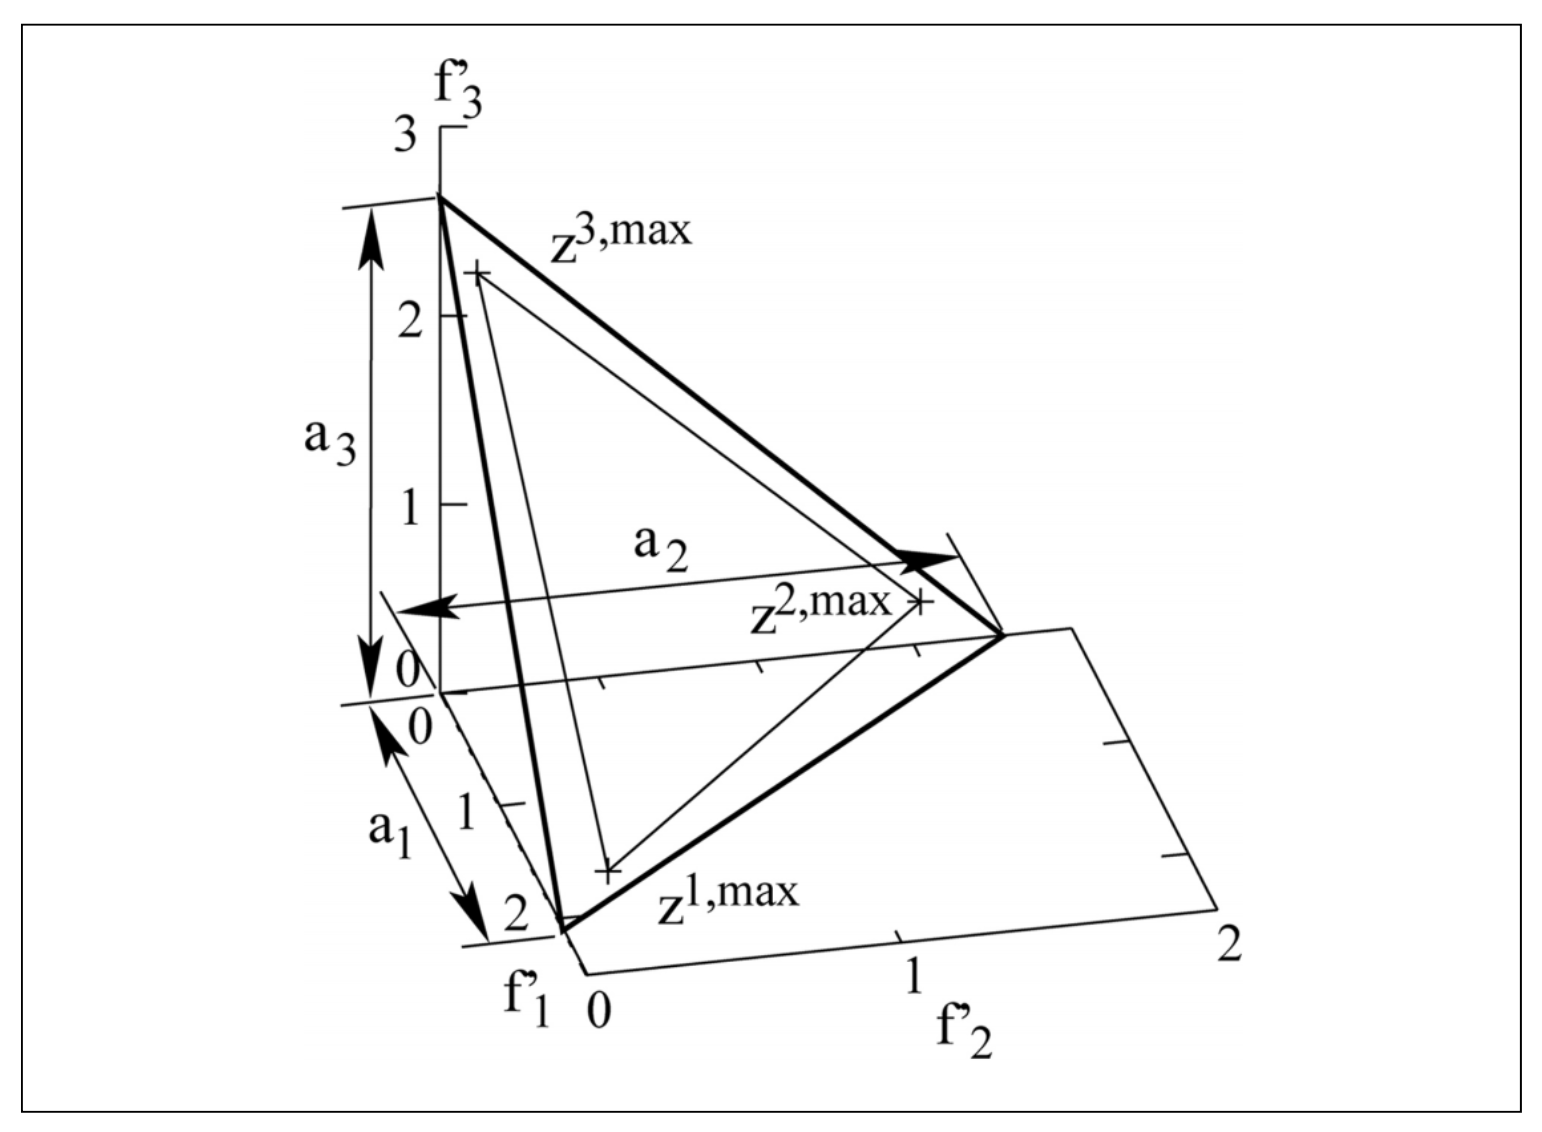
\includegraphics[scale=0.38]{literature_review/intercepts_nsga3.png}
    \caption{Procedure for computing intercepts and then forming the hyper-plane from extreme points. Shown for a three objective problem. \cite[~p.~582]{deb_evolutionary_2014}}
    \label{fig:intercepts_nsga3}
\end{figure}
\subsubsection{U-NSGA-III}\label{sec:unsga3}
\cite[~p.~361]{seada_unified_2016} extend the original NSGA-III algorithm to unify mono-objective, bi-objective, and many-objective problems. They do this by including a tournament selection procedure to select the parents $P_t$. For multi-objective problems (two or three objectives), if the population size $N$ is greater than the number of reference directions $H$, the reference directions have multiple population members for each reference direction. The non-dominated sorting divides the population into multiple non-dominated fronts. The selection procedure introduced by U-NSGA-III will emphasise:
\begin{enumerate}
    \item ``Non-dominated solutions over dominated solutions'' \cite[~p.~362]{seada_unified_2016}
    \item ``Solutions closer to reference directions over other non-dominated but distant solutions from the reference directions'' \cite[~p.~363]{seada_unified_2016}
\end{enumerate}
Compared with NSGA-II, in U-NSGA-III, the distribution of $(N - H)$ population members do not need a good diversity among them. Only $H$ population members closest to $H$ reference directions will have a well-spaced diversity. Although, since the user stated to find $H$ solutions, the additional $(N - H)$ population members make the algorithm more efficient by finding exactly $H$ Pareto-optimal points.
\\
Nevertheless, when the chosen $N$ is very close or equal to $H$, the algorithm may not obtain a solution for every reference direction in the early generations. However, since the tournament selection introduces selection pressure, the algorithm emphasises finding a single population member for each reference direction.

Algorithm \ref{alg:u_nsga3_select} shows the tournament selection procedure added to U-NSGA-III, based on \cite[~p.~362]{seada_unified_2016}. Furthermore, Algorithm \ref{alg:nsga3_unsga3} shows the full NSGA-III algorithm with optional unification, based on \cite{deb_evolutionary_2014} and \cite{seada_unified_2016}.
% The full NSGA-III algorithm with optional unification
\begin{algorithm}
    \caption{U-NSGA-III tournament selection procedure}\label{alg:u_nsga3_select}
    \SetKwInOut{Input}{Input}
    \SetKwInOut{Output}{Output}
    \Input{Two parents: $p_1$ and $p_2$.}
    \Output{The selected individual $p_s$.}
    \eIf{$p_1$ and $p_2$ are feasible}{
        \uIf{Rank of $p_1$ < Rank of $p_2$}{
            $p_s \gets p_1$;
        }{\uElseIf{Rank of $p_2$ < Rank of $p_1$}{
                $p_s \gets p_2$;
        }{\uElseIf{Perpendicular distance $d^{\perp}(p_1)$ < Perpendicular distance $d^{\perp}(p_2)$}{
                $p_s \gets p_1$;
            }{\Else{$p_s \gets p_2$;}}
            }
        }
    }{$p_s \gets \text{RandomSelection}(p_1, p_2)$;}
\end{algorithm}
\begin{algorithm}
    \caption{The combination of the NSGA-III and U-NSGA-III algorithms for a single generation $t$}\label{alg:nsga3_unsga3}
    \SetKwInOut{Input}{Input}
    \SetKwInOut{Output}{Output}
    \Input{A set of reference points $Z^s$, the parent population $P_t$, a boolean to use the U-NSGA-III selection procedure $U$.}
    \Output{The new population $P_{t+1}$.}
    $S_t \gets \emptyset$;\\
    $i \gets 1$;\\
    \eIf{$U = \text{True}$}{
        Apply the tournament selection described in Algorithm \ref{alg:u_nsga3_select}:\\
            \qquad $P'_t \gets$ TournamentSelection($P_t$);\\
        $Q_t \gets$ Crossover+Mutation($P'_t$);
    }{$Q_t \gets$ Crossover+Mutation($P_t$);}
    $R_t \gets P_t \cup Q_t$;\\
    $\mathbf{F} \gets$ non-dominated-sort($R_t$);\\
    \While{$|S_t| \leq N$}{
        $S_t \gets S_t \cup F_i$;\\
        $i \gets i + 1$;\\
    }
    Last front included in $S_t$: $F_l \gets F_i$;\\
    \eIf{$|S_t| = N$}{
        $P_{t+1} \gets S_t$;\\
        \Return $P_{t+1}$
    }{
        $P_{t+1} \gets$ Apply the procedure given in Algorithm \ref{proc:crowding_nsga3}. 
    }
    \Return{$P_{t+1}$}
\end{algorithm}
\clearpage
\subsection{Constrained multi-objective optimisation using a two-archive evolutionary algorithm (C-TAEA)}\label{sec:ctaea}
\cite{li_two-archive_2019} focus on the design of evolutionary algorithms for constrained multi-objective optimisation problems (CMOP). The authors propose a two-archive evolutionary algorithm, C-TAEA, which focuses on the \emph{convergence}, \emph{diversity}, and \emph{feasibility} of the solutions. The convergence-oriented archive (CA) tries to maintain the convergence and feasibility of the evolution process. In addition, it also provides selection pressure towards the Pareto-optimal front. Similarly, the diversity-oriented archive (DA) maintains convergence and diversity. In particular, it explores the areas of the feasible region that the CA has not exploited, which improves the population's diversity and helps jump over the local optima. Furthermore, the authors add a restricted mating selection mechanism that ``selects the appropriate mating parents from the CA and DA seperately according to their evolution status'' \cite[~p.~304]{li_two-archive_2019}.

\cite{li_two-archive_2019} introduce the association operator, which, similar to NSGA-III, calculates the perpendicular distance of each population member $s \in S$ to each reference line $u \in Z^s$. It then associates every individual of $S$ to the reference point (or subregion) with the closest reference line. The CA first pushes the population towards a feasible region and then tries to balance the convergence and diversity inside of the feasible region. Algorithm \ref{alg:CA} shows the procedure outlined in \cite[~pp.~306-307]{li_two-archive_2019}. Note that \cite{li_two-archive_2019} propose a process to improve the population diversity and to identify the worst solution $\mathbf{x}^w$ (line $16$ -- $19$ in Algorithm \ref{alg:CA}). First, calculate the distance between each solution $\mathbf{x} \in \pi_i$ and its nearest neighbour,
\begin{equation}
    dist(\mathbf{x}) = \min_{\substack{\mathbf{x'} \in \pi_i \\ \mathbf{x} \neq \mathbf{x'}}} \left\{\lVert \mathbf{x} - \mathbf{x'} \rVert_2 \right\}
\end{equation}
Subsequently, the temporary archive $S_d$ stores the solutions having the smallest distance and the definition of $\mathbf{x}^w$ is then,
\begin{equation}
    \mathbf{x}^w = \argmax_{\mathbf{x} \in S_d} \left \{ g^{tch}(\mathbf{x} | \mathbf{z^{ideal}, w^i}) \right \}
\end{equation}
where
\begin{equation}
    g^{tch}(\mathbf{x} | \mathbf{z^{ideal}, w^i}) = \max_{1 \leq j \leq K} \left \{ \frac{|f_j (\mathbf{x} - z^{ideal}_j|}{w^i_j} \right \}, \enspace \text{where} \enspace w^i \in (0, 1]
\end{equation}
The DA, on the other hand, aims to provide as many diversified solutions as possible. Its update mechanism has two main characteristics \cite[~p.~307]{li_two-archive_2019}:
\begin{enumerate}
    \item It does not consider the constraint violation.
    \item It takes the population outputted by the CA and complements the behaviour of the CA by exploring the under-exploited areas.
\end{enumerate}
The algorithm iteratively investigates each subregion, $\pi_i$, and decides the survival of the solutions in $H^d$. It makes these decisions by reviewing how many solutions exist in $P^c$ at $\pi_i$. Moreover, if $iter$ solutions exist in $P^c$ at $\pi_i$, then no solution in $H^d$ will be considered to survive at $\pi_i$ for this iteration. Otherwise, it chooses the best non-dominated solutions of $H^d$ at $\pi_i$ to survive \cite[~p.~307]{li_two-archive_2019}. Algorithm \ref{alg:DA} shows the full procedure of the DA taken from \cite[~p.~308]{li_two-archive_2019}.

For the offspring generation, the mating selection leverages the principal information from both archives. It combines both archives into one archive, $H_m$, and then checks the proportion of non-dominated solutions for each archive in $H_m$. If there is a higher proportion for archive CA, it means that the convergence status of the CA is better than the DA, and the first parent gets selected using a tournament selection procedure from the CA archive based on feasibility. Otherwise, the first parent gets selected the same way but from the DA archive. \cite[~p.~307-308]{li_two-archive_2019}
\\\\
For the second mating parent, whether chosen from the CA or DA archives depends on the proportion of non-dominated individuals in the CA archive. The more non-dominated solutions the CA archive has, the higher the probability of the second parent coming from the CA archive and the lower the probability of it coming from the DA archive. \cite[~p.~308]{li_two-archive_2019}
\\\\
The tournament selection procedure of the C-TAEA is feasibility-driven. Principally, if the randomly selected candidates are feasible, they are chosen based on Pareto dominance. However, if only one of the candidates is feasible, the feasible one is chosen. Otherwise, a random selection occurs between both candidates. \cite[~p.~308]{li_two-archive_2019}

\begin{algorithm}
    \caption{DA update procedure for a single generation $t$}\label{alg:DA}
    \SetKwInOut{Input}{Input}
    \SetKwInOut{Output}{Output}
    \SetKw{Break}{break}
    \Input{The convergence archive population $P_t^c$, the diversity archive population $P_t^d$, the offspring population $Q_t$, and a set of reference directions $Z^s$}
    \Output{The updated diversity archive population $P_{t+1}^d$}
    $S \gets \emptyset, \enspace iter \gets 1$;\\
    Create the hybrid population $H_d$\\
    \quad $H^d \gets P_t^d \cup Q_t$;\\
    $\pi_d \gets Associate(H^d, Z^s)$;\\
    $\pi_c \gets Associate(P_t^c, Z^s)$;\\
    \While{$|S| < N$}{
        \For{$i \gets 1$ \KwTo $N$}{
            \If{$|\pi_c^i| < iter$}{
                \For{$j \gets 1$ \KwTo $iter - |\pi_c^i|$}{
                    \If{$\pi_d^i \neq \emptyset$}{
                        $O^i \gets$ non-dominated-sorting($H^d_{\pi_d^i}$);\\
                        $\mathbf{x}^{best} \gets \argmin_{\mathbf{x} \in O^i} \left \{g^{tch}(\mathbf{x} \: | \: \mathbf{z^*, Z^s_c}) \right \}$; \\
                        $\pi^i_d \gets \pi^i_d \backslash x^{best}$;\\
                        $S \gets S \cup x^{best}$;
                    }
                    \Else{\Break}
                }
            }
        }
        $iter \gets iter + 1$;
    }
    $P^d_{t+1} \gets S$;\\
    \Return{$P^d_{t+1}$}
\end{algorithm}
\begin{algorithm}
    \caption{CA update procedure for a single generation $t$}\label{alg:CA}
    \SetKwInOut{Input}{Input}
    \SetKwInOut{Output}{Output}
    \Input{The convergence archive population $P_t^c$, the offspring population $Q_t$, and a set of reference directions $Z^s$}
    \Output{The updated convergence archive population $P_{t+1}^c$}
    $S \gets \emptyset, \enspace S_c \gets \emptyset$, $i \gets 1$;\\
    Create the hybrid population $H_c$\\
    \quad $H_c \gets P_t^c \cup Q_t$;\\
    Add the feasible solutions in $H_c$ to a temporary archive $S_c$\\
    \uIf{$|S_c| = N$}{
        $P_{t+1}^c \gets S_c$;\\
    }\uElseIf{$|S_c| > N$}{
        $\mathbf{F} \gets$ non-dominated-sort($S_c$);\\
        \While{$|S| < N$}{
            $S \gets S \cup F_i$;\\
            $i \gets i + 1$;
        }
        \If{$|S| > N$}{
            $\pi$ = $Association(S, \enspace Z^s)$ as in Algorithm \ref{proc:crowding_nsga3};\\
            \While{$|S| > N$}{
                Find the most crowded subregion (or reference point) $\pi_i$\\
                \ForEach{$\mathbf{x} \in \pi_i$}{
                        dist($\mathbf{x}$) $\gets$ $\min_{\substack{\mathbf{x'} \in \pi_i \\ \mathbf{x} \neq \mathbf{x'}}}$ $\lVert \mathbf{x} - \mathbf{x'} \rVert$;
                    
                }
                $S_d \gets \argmin_{\mathbf{x} \in \pi_i} \left\{dist(\mathbf{x}) \right\}$;\\
                $\mathbf{x}^w \gets \argmax_{\mathbf{x} \in S_d} \left\{g^{tch}(\mathbf{x}| \mathbf{z^{ideal}, Z^s_i})\right\}$;\\
                $S \gets S \backslash \mathbf{x}^w $
            }
        }
        $P_{t+1}^c \gets S$
    }\Else{
        $S_I \gets H_c \backslash S_c$;\\
        $\mathbf{F} \gets$ non-dominated-sort($S_I$);\\
        \While{$|S_c| < N$}{
            $S \gets S \cup F_i$;\\
            $i \gets i + 1$;
        }
        Remove large infeasible solutions from $S$. $CV$ is the constraint violation. \\ 
        \While{$|S| > N$}{
            $\mathbf{x}^w \gets \argmax_{\mathbf{x} \in F_{i - 1}} \{CV(\mathbf{x}) \}$;\\
            $S \gets S \backslash \mathbf{x}^w$;
        }
        $P_{t+1}^c \gets S$
    }
    \Return{$P_{t+1}^c$}
\end{algorithm}
\clearpage
\subsection{Adaptive Evolutionary Algorithm based on Non-Euclidean Geometry (AGE-MOEA)}\label{sec:agemoea}
\cite{panichella_adaptive_2019} proposes a different approach to the crowding distance operator first proposed in NSGA-II while keeping the original framework of NSGA-II. It implements a survival score that ``combines diversity and proximity of the non-dominated fronts'' \cite[~p.~596]{panichella_adaptive_2019}. First, the author proposes a fast heuristic that estimates the geometry of the first non-dominated front, $F_1$, in each generation and then computes the proximity as the "distance between each population member and the ideal point" \cite[~p.~596]{panichella_adaptive_2019}.
\\\\
The diversity calculation uses the distance between the population members. The distance to compute the proximity and diversity corresponds to the $L_p$ norm, whose exponent $p$ depends on the geometry of the optimal Pareto front. Since the optimal Pareto front is unknown, the computation of $p$ depends on each generation's geometry of $F_1$.
\begin{definition}[The $L_p$ norm (\cite{thompson_minkowski_1996})]
In a $K$-dimensional space $\mathbb{R}^K$, let $v$ be a vector of size $K$, i.e. $v = (v_1,...,v_K)$. Then the $L_p$ norm of $v$ in the $K$-dimensional space is defined by,
\begin{equation}
    \lVert v \rVert_p = (v_1^p + ... + v_K^p)^{1/p}, \quad p \geq 1
\end{equation}
\qed
\end{definition}

\cite[~p.~597]{panichella_adaptive_2019} uses the same normalisation technique found in NSGA-III. However, it occurs only on the first non-dominated front. Therefore, the objectives of $F_1$ take on values between $[0,1]$, and the objectives for the other non-dominated fronts, $F_{d > 1}$, can have values greater than one.
\\\\
In order to determine the geometry of the first non-dominated front, $F_1$, we have to find the value $p$ of the $L_p$ norm such that the corresponding unit hypersurface best fits the normalised objectives of the front $F_1$. The optimal hypersurface has an $L_p$ norm where all points in the normalised objectives are equally distant from the ideal points. 

It turns out that the extreme points in the front correspond to the intersections of the front with the objective axes \cite[~p.~598]{panichella_adaptive_2019}. I.e. the intersection point of $F_1$ with axis $f_i ^n$ has the objective value $f_i^n = 1$, and all other objectives $f_j^n$ have the objective value $f_j^n = 0 \enspace \forall \: j \neq i$.  Thus the distance from the intersection point, $a_k$, to the ideal point, $z^{min}_k$, is always equal to one for any chosen $p$ exponent \cite[~p.~598]{panichella_adaptive_2019}.
The problem consists of solving the following system of non-linear equations.
\begin{equation}
    \left\{
    \begin{aligned}
      & \left(f_1(S_1)^p + ... + f_K(S_1)^p\right)^{1/p} = 1 \\
      & \qquad \qquad \: \: . \enspace . \enspace . \\
      & \left(f_1(S_m)^p + ... + f_K(S_m)^p\right)^{1/p} = 1 
    \end{aligned}
  \right.
\end{equation}
where $m$ is the number of points in the front $F_1$.
\\\\
\cite{panichella_adaptive_2019} approximates the value of $p$ by considering the central point in the first non-dominated front, $F_1$. As all the objectives are normalised, the central point $C$ is the point in $F_1$ with the lowest perpendicular distance to the vector $\vec{\beta}$ delimited by the nadir point $z^{max} = 1$ and the ideal point $z^{min} = 0$.
\begin{equation}
    C = \argmin_{f^n (S)} \left\{ d^{\perp}(f^n (S), \vec{\beta}) \right\}, \quad \forall \: S \in F_1
\end{equation}
\begin{figure}[ht]
    \centering
    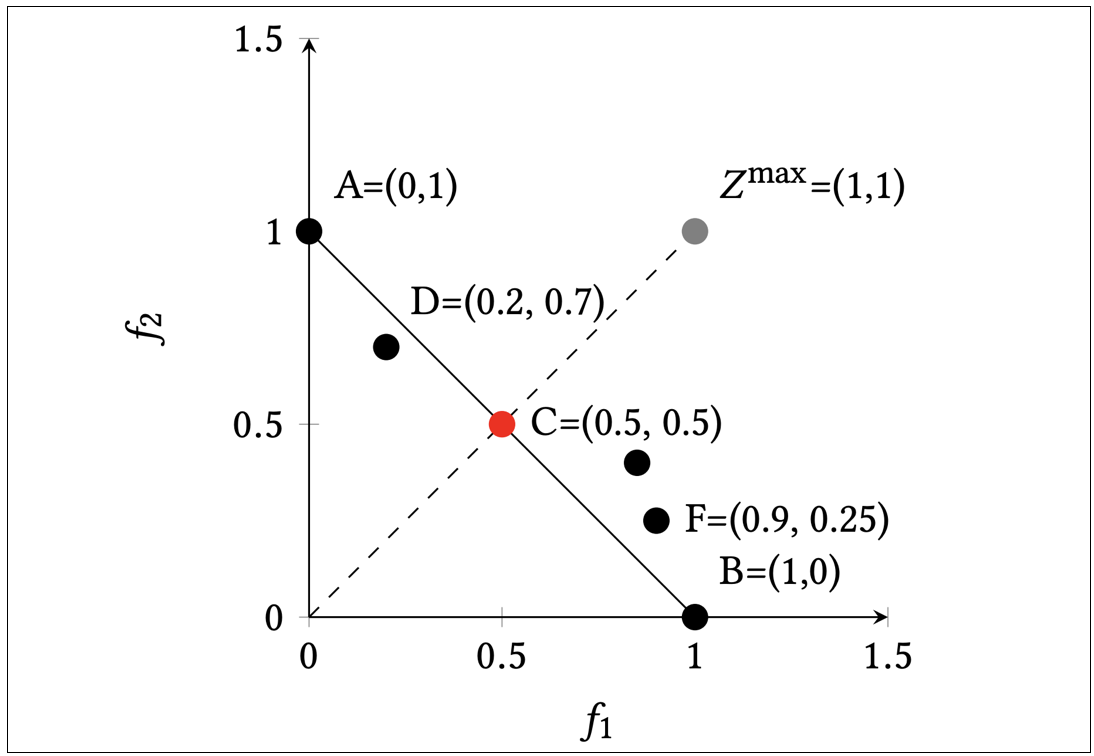
\includegraphics[scale=0.5]{literature_review/central_point.png}
    \caption{Example of the central point $C$ of the normalised non-dominated front.}
    \label{fig:central_point}
\end{figure}

Figure \ref{fig:central_point} shows an example from \cite[~p.~598]{panichella_adaptive_2019} for calculating the central point $C$. The figure depicts two extreme points, $A=(0,1)$ and $B=(1,0)$, that lie on two objective axes, $f^n_1$ and $f^n_2$, respectively. The central point $C$ situates on the vector $\vec{\beta}$. Considering only the extreme points, $A$ and $B$, and the central point, $C$, the problem consists of finding a $p$ such that the $L_p$ norm of $C$ equals to one. I.e. $(C_1^p + C_2^p)^{1/p} = 1.$ To find the value of $p$ where $C$ lies directly on the bisector of $\vec{\beta}$, we solve the following equation:
\begin{equation}
\begin{aligned}
\left(\sum_{i=1}^K C_i^p \right) = 1 \quad & \Rightarrow K \cdot C_1^p = 1 \\
    &\Rightarrow C_1^p = \frac{1}{K} \\
    &\Rightarrow p = -\frac{\log(K)}{\log(C_1)}
\end{aligned}
\end{equation}
However, the central point in the first non-dominated front, $F_1$, can have a distance $d^{\perp}(C,\vec{\beta}) > 0$; therefore, the objective space coordinates may not be identical. \cite[~p.~598]{panichella_adaptive_2019} thus approximates the value of the exponent $p$ using the following equation.
\begin{equation}
\begin{aligned}
    p &= - \frac{\log(K)}{\log(\frac{1}{K} \sum_{i=1}^K C_i)}\\
    &= - \frac{\log(K)}{\log(K) - \log(\sum_{i=1}^K C_i)}
\end{aligned}
\end{equation}

To measure the diversity and proximity of $S \in F_1$, we compute the minimum distance compared to the other solutions in $F_1$ and the distance of the objective vector $f^n$ to the ideal point, respectively. \cite[~p.~599]{panichella_adaptive_2019} writes that ``a solution $S$ with $proximity < 1$ dominates part of the unitary hypersurface of $L_p$'', which point D shows in Figure \ref{fig:central_point}, and "a solution $S$ with $proximity > 1$ is more distant from the ideal point compared to points in the unit hypersurface of $L_p$", which point F shows in Figure \ref{fig:central_point}. 

The survival score of the solutions $S \in F_1$ merges the diversity and proximity, where they need to be maximised and minimised, respectively.
\begin{equation}
    score(S) = \frac{diversity(S,F_1)}{proximity(S)}
\end{equation}
where $diversity$ and $proximity$ are:
\begin{alignat}{3}
    &diversity(S, F_1) &&= \min_{S' \neq S \in F_1} \lVert f^n(S) - f(S') \rVert_p \\
    &proximity(S) &&= \lVert f^n (S) - z^{ideal} \rVert_p = \lVert f^n(S) \rVert_p
\end{alignat}
\section{Conclusion}
In this chapter, we conveyed the literature related to this Thesis's goal. We started by showing the work done in the past in the scope of waste management, and we showed the main paper that we will improve to work with large-scale problems. Furthermore, we illustrated the novel model that \cite{olapiriyakul_multiobjective_2019} created and its constraints, which we will implement for the branch and cut and the evolutionary algorithm approach.
\\
After that, we gave some insight into the different evolutionary algorithms we will use in the subsequent chapters. These include, NSGA-II (Section \ref{sec:nsga2}), NSGA-III (Section \ref{sec:nsga3}), U-NSGA-III (Section \ref{sec:unsga3}), C-TAEA (Section \ref{sec:ctaea}), and AGE-MOEA (Section \ref{sec:agemoea}). NSGA-II uses a crowding sort technique, making the original NSGA algorithm much more computationally efficient. Furthermore, we gave the procedure of the various algorithms by providing the pseudocode.
\chapter[Methodology]{Methodology}
In this chapter, we extend the model proposed by \cite{olapiriyakul_multiobjective_2019} in section \ref{sec:wmo} by incorporating evolutionary algorithms to solve the proposed MILP problem faster, with a more diverse set of solutions, and on a larger scale. 
The following sections outline the data and methods used to support these claims. 
\section{Data}
The data plays a vital role in supporting the claims made throughout this Thesis. There is currently a minimal amount of publicly available data on this topic. In order to create a dataset that is as close as possible to the real world, we used the data provided by \cite{olapiriyakul_multiobjective_2019} in their case study of Pathum Thani in Thailand, which provided us with health impact data and data on land-usage impacts of the various facilities. Moreover, the authors also gave data on the vehicle capacities and the facility capacities. However, it did not provide data on the facilities' construction and operational costs. 
\\\\
For the different facilities' construction costs, we used the data given by the incinerator in Giubiasco, Ticino, Switzerland, \cite[~p.~7]{azienda_cantonale_dei_rifiuti_rapporto_nodate}. It states that the waste-to-energy plant subsidy in Giubiasco, Switzerland was $40$ million CHF in $2004$, $42'050'290$ CHF when adjusting for inflation for $2022$. As the area of the incinerator plant is $40'000 \: m^2$ square meters, the price per square meter is, thus, 1051.3 CHF. 
\\\\
For the landfill facilities, \cite{elrabaya_identifying_2021} identified the total cost to landfill municipal waste in Sharjah, UAE, in 2021. They additionally consider the costs to construct, manage, excavate and consult the creation of an MSW landfill. The sum of these costs is $6'482'949$ USD. Adjusting for inflation and converting to CHF, the total cost becomes $7'206'328.42$ CHF. The MSW landfill occupies an area of $126'500 \: m^2$ square meters. Thus the cost per square meter is $57$ CHF. Unfortunately, there was no publicly available data for the cost of constructing sorting facilities. For this reason, we chose to use the cost per square meter of a landfill facility and add an equipment cost budget depending on the size of the facility of $250'000$ CHF, $500'000$ CHF, and $750'000$ CHF for small, medium, and large sorting facilities, respectively.
\\\\
For the operational cost, as no publically available data exists, we choose uniformly distributed random numbers that increase depending on the size of the facility. We choose $\mathcal{U}(100'000, 200'000)$, $\mathcal{U}(200'000, 400'000)$, and $\mathcal{U}(400'000, 600'000)$, for facilities of size small, medium, and large, respectively.
\\
The DALY amounts seen in Table \ref{tab:fac_health} show the health impact per person. Thus, we add a uniformly random population number for every vertex, $V$, on the generated graph, $G$, $\mathcal{U}(35'000, 80'000)$. In addition, we add $720'000 \cdot U(0, 1)$ to the candidate nodes, as these should inhabit more people due to the larger land area. When calculating the population living near the facilities, which would be the affected area of the facility, we take the population of that node multiplied by the direct land usage of the facility of size $l$ in squared kilometres.
When calculating the population living near transport routes, we use the following equation, with $\alpha = \mathcal{U}(0.01, 0.05)$ and a graph $G = (V, E)$.
\begin{equation}
    P_{ij} = \alpha(1 - \alpha) \cdot (\lVert V^i - V^j \rVert_2 \cdot (V^i_{P} + V^j_{P}))
\end{equation}
The population on the link $ij$ is adapted based on the population at vertice $i$ and vertice $j$.
\begin{table}[ht]
\centering
\resizebox{\textwidth}{!}{%
\begin{tabular}{ccccccc}
\hline
 & \multicolumn{3}{c}{\textbf{Direct land use ($\mathbf{m^2}$)}} & \multicolumn{3}{c}{\textbf{Indirect land use ($\mathbf{m^2}$)}} \\
Waste facility & Small size & Medium size & Large size & Small size & Medium size & Large size \\ \hline
Sorting facility & $4'800$ & $8'000$ & $16'000$ & $6'191$ & $10'780$ & $21'559$ \\
Incinerator facility & $8'000$ & $16'000$ & $24'000$ & $11'971$ & $23'941$ & $35'911$ \\
Landfill facility & $80'000$ & $160'000$ & $192'000$ & $127'770$ & $255'525$ & $335'295$ \\ \hline
\end{tabular}%
}
\caption{Direct and indirect land use impacts (Taken from \cite[~p.~8]{olapiriyakul_multiobjective_2019})}
\label{tab:my-landuse}
\end{table}

\begin{table}[ht]
\centering
\resizebox{\textwidth}{!}{%
\begin{tabular}{@{}cllllcllllcllllcl@{}}
\toprule
\textbf{Waste facility} &  &  &  &  & \textbf{Size} &  &  &  &  & \textbf{Capacity (tonne/day)} &  &  &  &  & \textbf{DALYs} &  \\ \midrule
 &  &  &  &  & Small &  &  &  &  & $50$ &  &  &  &  & $0.07$ &  \\
Sorting facility &  &  &  &  & Medium &  &  &  &  & $100$ &  &  &  &  & $0.14$ &  \\
 &  &  &  &  & Large &  &  &  &  & $300$ &  &  &  &  & $0.28$ &  \\ \midrule
 &  &  &  &  & Small &  &  &  &  & $50$ &  &  &  &  & $5.95$ &  \\
Incinerator facility &  &  &  &  & Medium &  &  &  &  & $100$ &  &  &  &  & $11.9$ &  \\
 &  &  &  &  & Large &  &  &  &  & $150$ &  &  &  &  & $17.85$ &  \\ \midrule
 &  &  &  &  & Small &  &  &  &  & $50$ &  &  &  &  & $3.89$ &  \\
Landfill facility &  &  &  &  & Medium &  &  &  &  & $100$ &  &  &  &  & 7.78 &  \\
 &  &  &  &  & Large &  &  &  &  & $150$ &  &  &  &  & $11.66$ &  \\ \bottomrule
\end{tabular}%
}
\caption{Facility impact on public health. (Adapted from \cite[~p.~8]{olapiriyakul_multiobjective_2019})}
\label{tab:fac_health}
\end{table}

\begin{table}[ht]
\centering
\resizebox{\textwidth}{!}{%
\begin{tabular}{@{}ccccccccccccccc@{}}
\toprule
\textbf{Fleet types} &  &  &  &  &  &  & \textbf{Capacity (ton)} &  &  &  &  &  &  & \textbf{DALYs full load (per tkm)} \\ \midrule
Light truck &  &  &  &  &  &  & $16$ &  &  &  &  &  &  & $5.62 \cdot 10^{-8}$ \\
Heavy truck &  &  &  &  &  &  & $32$ &  &  &  &  &  &  & $1.12 \cdot 10^{-7}$ \\ \bottomrule
\end{tabular}%
}
\caption{Transportation impact on public health (Adapted from \cite[~p.~9]{olapiriyakul_multiobjective_2019})}
\label{tab:link_health}
\end{table}


\begin{table}[ht]
\centering
\resizebox{\textwidth}{!}{%
\begin{tabular}{@{}lllcllcllcl@{}}
\toprule
\multicolumn{11}{c}{\textbf{Construction cost}} \\
Waste facility &  &  & Small size (CHF) &  &  & Medium size (CHF) &  &  & Large size (CHF) &  \\ \midrule
Sorting facility &  &  & $523'600$ &  &  & $956'000$ &  &  & $1'662'000$ &  \\
Incinerator facility &  &  & $8'410'400$ &  &  & $16'820'800$ &  &  & $25'231'200$ &  \\
Landfill facility &  &  & $4'560'000$ &  &  & $9'120'000$ &  &  & $10'944'000$ &  \\ \bottomrule
\end{tabular}%
}
\caption{Facility construction costs.}
\label{tab:const_oper_costs}
\end{table}
\clearpage
\section{Evolutionary algorithms}
This section proposes an adaptation to the evolutionary algorithms' crossover and mutation operators to solve the MILP problem proposed by \cite{olapiriyakul_multiobjective_2019}. In order to select only the best candidate cities, we have to add zeroes into the solutions of the evolutionary algorithm in such a way that we narrow the search space to feasible solutions and lead the algorithm to the global optimum. We achieve this by implementing an adapted version to the crossover and mutation operators and adding a repair operator that can alter the solutions to explore the feasible region. 
\subsection{Binary decision variables $y$}\label{sec:bin_dec_var}
For the binary decision variable crossover, we first apply a single-point crossover and then apply the procedure shown in figures \ref{fig:binary_crossover_two} and \ref{fig:binary_crossover_three}. We sample random columns with replacements for each row, slowly bringing the search space to a feasible region.  Afterwards, we set each row's selected column to zero to improve the solution space slowly.
\begin{figure}[ht]
    \centering
    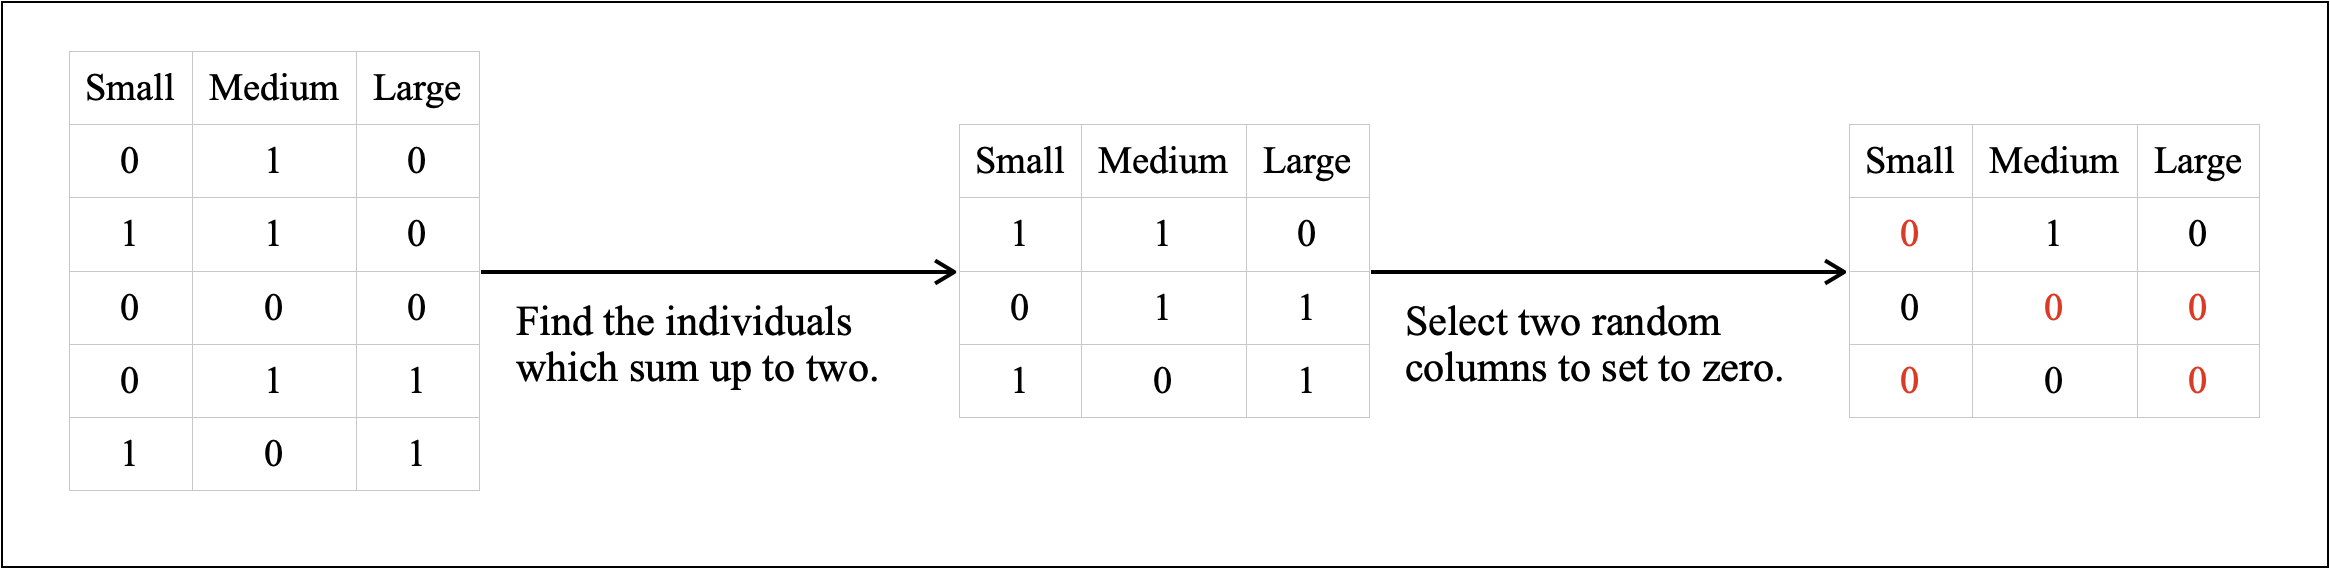
\includegraphics[width=\linewidth]{methodology/binary_crossover_operator_two.png}
    \caption{Method for the binary decision variable crossover, for individuals that sum to two.}
    \label{fig:binary_crossover_two}
\end{figure}
% \newpage
\begin{figure}[ht]
    \centering
    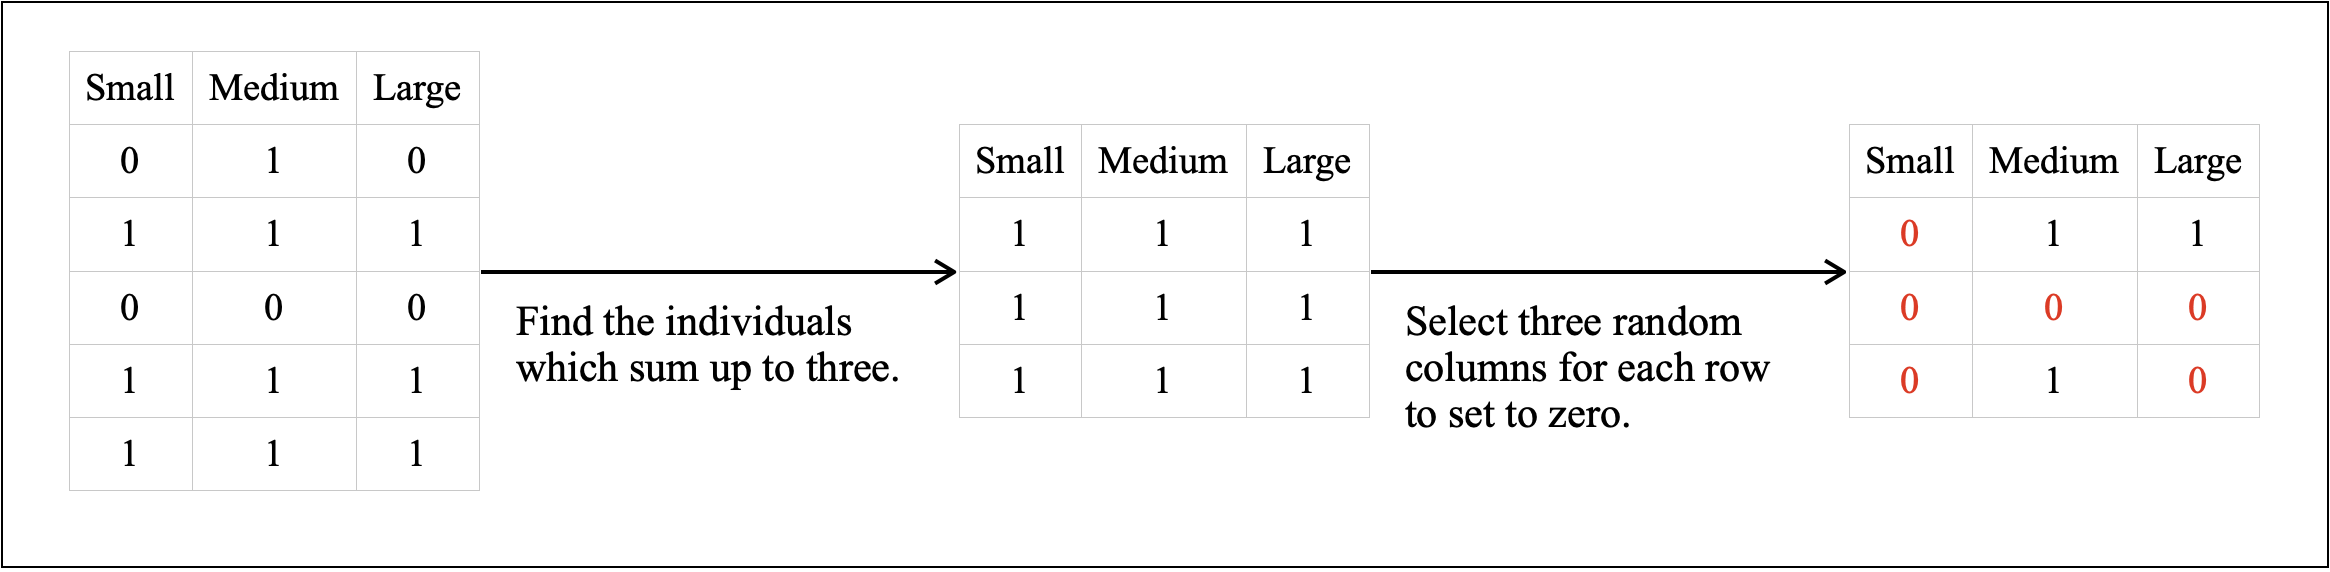
\includegraphics[width=\linewidth]{methodology/binary_crossover_operator_three.png}
    \caption{Method for the binary decision variable crossover, for individuals that sum to three.}
    \label{fig:binary_crossover_three}
\end{figure}

Figure \ref{fig:binary_mutation} shows the adaptation of the mutation operator by performing a typical binary mutation and then setting the non-mutated one values to zero in the rows that had a mutated one value. This mutation operator slowly moves the solution space into the feasible region and can explore newly mutated individuals by staying in the feasible region. 
\begin{figure}[ht]
    \centering
    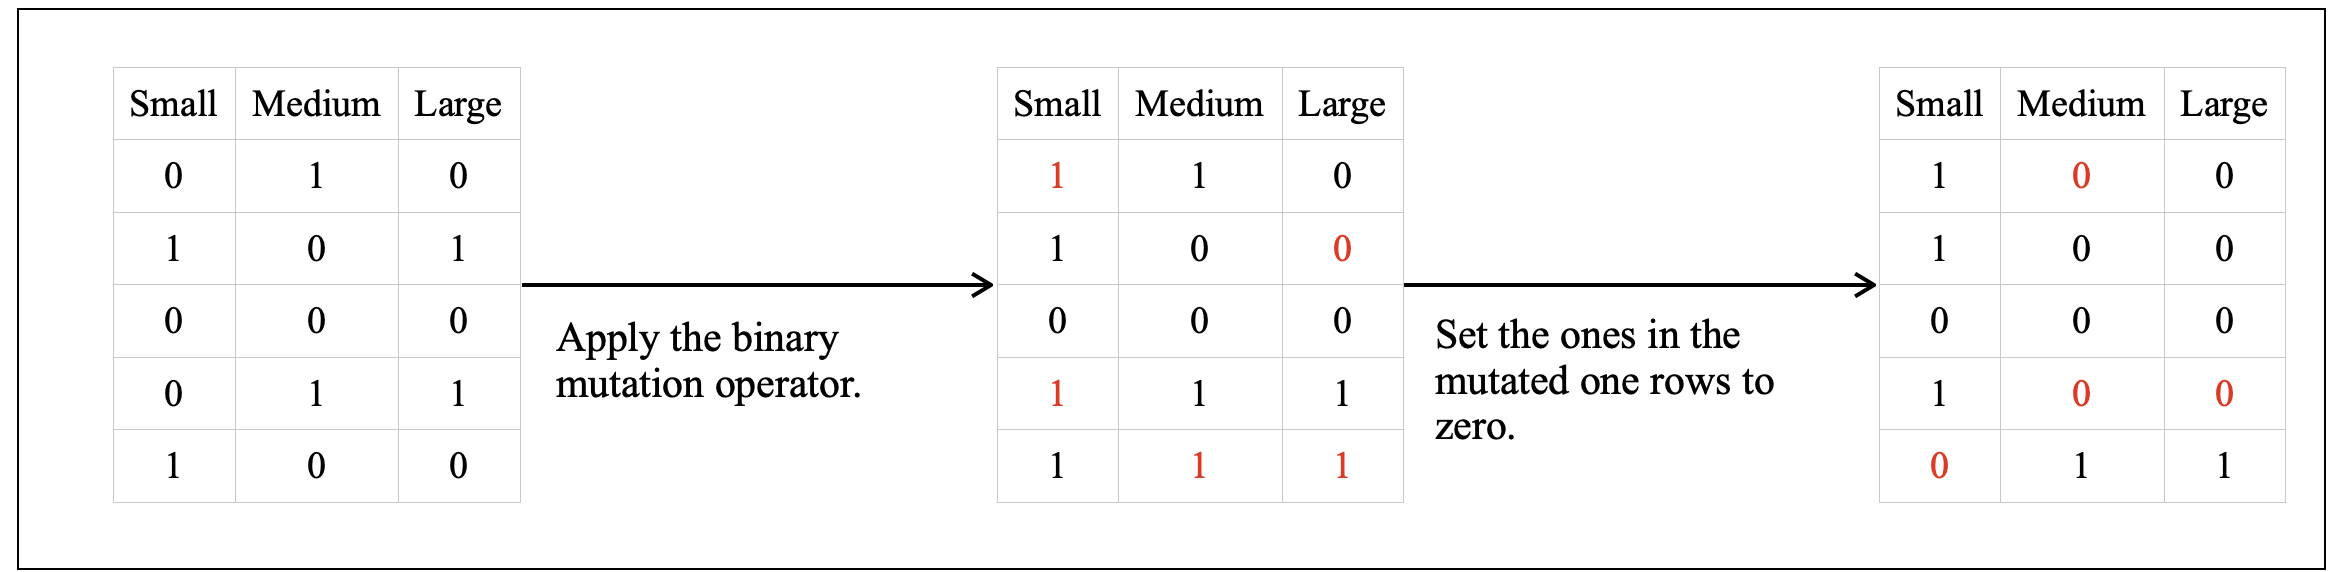
\includegraphics[width=\linewidth]{methodology/binary_mutation_operator.png}
    \caption{Method for the binary decision variable mutation.}
    \label{fig:binary_mutation}
\end{figure}
\\
Algorithm \ref{alg:bin_update} gives the pseudocode for the binary $y$ update procedure. We first apply the single-point crossover on the population, receiving a matrix of shape $|C| \times l_{size}$, which for example, would be of size $6 \times 3$, for an average city count of $2$, as we would have $6$ total candidate cities and $3$ total facility sizes. \\
After that, we obtain the rows where the sum equals $M$, the sum of the rows to identify. We then sample random integers of size $M$ for each row found and set the row and column combination to zero.
\\\\
For the mutation, we sample points uniformly at random for all decision variables and create a copy of the population called $P_{copy}$. We then obtain the decision variables to flip and not to flip. After that, we mutate the decision variables in our flip category by applying a not operator for these in $P_{copy}$. Looking at the copied population, we will have some variables flipped to ones and some to zero. We select the flipped variables that equal one and set the row to zero in the original population. Then we overwrite the non-flipped variables in the copied population with the original population.
\begin{algorithm}
\caption{$y$ update procedure for one generation $t$}\label{alg:bin_update}
\SetKwInOut{Input}{Input}
\SetKwInOut{Output}{Output}
\Input{The probability of mutation $p$, probability of crossover $c$, population $P$, candidate sorting facilities $J$, candidate incinerator facilities $K$, and candidate landfill facilities $K'$.}
\Output{The binary crossover result $X$.}
\textbf{Crossover operator}:\\
$l_{size} \gets \sum L(J) \cap L(K) \cap L(K')$;\\
$C \gets J \cup K \cup K'$;\\
$X_{|C| \times l_{size}} \gets$ single-point-crossover($P$, $c$);\\
\For{($M = 2;\ M < 4;\ M = M + 1$)}{
$\delta$ = $\begin{cases} 
    1 & if \: \sum_{j = 1}^{l_{size}} X_{ij} = M, \quad \forall i \in C; \\
    0 & otherwise
\end{cases}$\\
$\alpha \gets$ Sample random integers with replacement of size $\delta_{\delta = 1} \times M$; \\
$X_{\delta, \alpha} \gets 0$;\\}
$P \gets X$;\\
\textbf{Mutation operator}:\\
\emph{Obtain probabilities uniformly for all binary variables}:\\
$Z \gets Z \in U[0,1]^{ij}, \quad \forall i, j \in P$;\\
$P^{copy} \gets copy(P)$;\\
\emph{Get the variables to be mutated and not mutated:}\\
$flip \gets Z < p$;\\
$not \: flip \gets Z \geq p$;\\
\emph{Apply a not operator on the variables to be flipped and add them to the copied population}:\\
$P^{copy}_{flip} \gets \neg P_{flip}$;\\
\emph{Set the rows of the flipped to one variables to zero in the original population:}\\
$P^i_{P^{copy}_{flip, ij} = 1} \gets 0, \quad \forall i, j \in P$\\
\emph{Overwrite the non-flipped variables in the copied population:}\\ 
$P^{copy}_{not \: flip} \gets P_{not \: flip}$\\
\Return{$P^{copy}$}
\end{algorithm}
\clearpage
\subsection{Real decision variables $f$} \label{sec:real_dec_variables}
Equation \ref{eq:general_matrix} shows the general matrix of the real number decision variables, f, where it conveys the amount of waste sent from collection centres $i$ to sorting facilities $j$, where $n \in \mathbb{N}$ is the average amount of centres available. 


\begin{equation}\label{eq:general_matrix}
    F_{n \times n} =
  \left[ {\begin{array}{cccc}
    f_{i_1, j_1} & f_{i_1, j_2} & \cdots & f_{i_1, j_n}\\
    f_{i_2, j_1} & f_{i_2, j_2} & \cdots & f_{i_2, j_n}\\
    \vdots & \vdots & \ddots & \vdots\\
    f_{i_n, j_1} & f_{i_n, j_2} & \cdots & f_{i_n, j_n}\\
  \end{array} } \right]
\end{equation}

In order to satisfy the hard constraint \ref{outflow}, we have to normalise the matrix $F$ by dividing each row by the amount of supply at collection centre $i$. This normalisation will allow us to make the sum of each row one and satisfy constraint \ref{outflow}. We achieve this by applying equation \ref{eq:sum_to_one} to each row of the normalised matrix $F$. 
\begin{equation}\label{eq:sum_to_one}
    F_i = \frac{F_{i}}{\sum_{j = 1}^{n} f_{ij}}, \quad \forall i \in I
\end{equation}
We apply this procedure in the real number single-point crossover operator and the mutation operator to quickly satisfy constraint \ref{outflow} without spending time on infeasible solutions.
For constraint \ref{flow_balance}, we apply the same procedure; however, we use a matrix that combines the incinerator and landfill real numbers, as seen in the matrix of equation \ref{eq:inc_land_matrix}. We normalise the rows by taking the sum of each column of the matrix in equation \ref{eq:general_matrix}. Then we divide each row by the sum of that row to obtain a sum equal to one (equation \ref{eq:sum_inc_one}). 
\begin{equation}\label{eq:inc_land_matrix}
    \newcommand{\vphB}{\vphantom{\Big\{}}
  \newcommand{\addlinegap}[1][\jot]{\\\\[\dimexpr-\normalbaselineskip+#1]}
  F_{n \times 2n} = 
  \left[ \begin{array}{@{}c@{}c@{}c@{}c@{}}
    \vphB \addlinegap \vphB \addlinegap \vphB \addlinegap \vphB
  \end{array} \right.\kern-\nulldelimiterspace
  \overbrace{\begin{array}{@{}c@{}c@{}c@{}}
    \vphB f_{j_1, k_1} \addlinegap f_{j_2, k_1} \addlinegap \vdots \addlinegap f_{j_n, k_1}
  \end{array}
  \hspace{\arraycolsep}
  \begin{array}{@{}c@{}}
    \vphB f_{j_1, k_2} \addlinegap f_{j_2, k_2} \addlinegap \vdots \addlinegap f_{j_n, k_2}
  \end{array}
  \hspace{\arraycolsep}
  \begin{array}{@{}c@{}}
    \vphB \cdots\addlinegap \cdots \addlinegap \ddots \addlinegap \cdots
  \end{array}
  \hspace{\arraycolsep}
  \begin{array}{@{}c@{}}
    \vphB f_{j_1, k_n} \addlinegap f_{j_2, k_n} \addlinegap \vdots \addlinegap f_{j_n, k_n}
  \end{array}}^K
    \hspace{\arraycolsep}
  \overbrace{\begin{array}{@{}c@{}c@{}c@{}}
    \vphB f_{j_1, k'_1} \addlinegap f_{j_2, k'_1} \addlinegap \vdots \addlinegap f_{j_n, k'_1}
  \end{array}
  \hspace{\arraycolsep}
  \begin{array}{@{}c@{}}
    \vphB f_{j_1, k'_2} \addlinegap f_{j_2, k'_2} \addlinegap \vdots \addlinegap f_{j_n, k'_2}
  \end{array}
  \hspace{\arraycolsep}
  \begin{array}{@{}c@{}}
    \vphB \cdots\addlinegap \cdots \addlinegap \ddots \addlinegap \cdots
  \end{array}
  \hspace{\arraycolsep}
  \begin{array}{@{}c@{}}
    \vphB f_{j_1, k'_n} \addlinegap f_{j_2, k'_n} \addlinegap \vdots \addlinegap f_{j_n, k'_n}
  \end{array}}^{K'}
  \kern-\nulldelimiterspace\left.\begin{array}{@{}c@{}c@{}c@{}}
    \vphB \addlinegap \vphB \addlinegap \vphB \addlinegap \vphB
  \end{array} \right]
\end{equation}
  
\begin{equation}\label{eq:sum_inc_one}
    F_j = \frac{F_j}{\sum_{k = 1}^{2n} f_{jk}}, \quad \forall j \in J
\end{equation}
\\\\
In order to close facilities while staying in the feasible region of the constraints, we add a repair operator that repairs the solutions after the crossover and mutation operators. The proposed approach adds zeroes to the integer, $x$, and real, $f$, numbered decision variables. We achieve this by setting the columns to zero, where the sum of the rows of the binary decision variable, $y$, is zero. In addition, we also set the values of $f$ to zero where $x$ is zero and vice versa. Afterwards, we use the same normalisation and division approach as in the real numbered, $f$, crossover and mutation to fix constraints \ref{outflow} and \ref{flow_balance}. We then denormalise by multiplying the rows of $f$ by the supply at collection centre $i$ and fix the integer-numbered values, $x$, by applying equation \ref{eq:int_solving} to fix constraint \ref{transportation_capacity_ij}. To fix constraints \ref{transportation_capacity_jk} and \ref{transportation_capacity_jk_prime}, we apply the same equation for links $jk$ and $jk'$. 
\begin{equation}\label{eq:int_solving}
    x_{ij} = \left\lceil \frac{f_{ij}}{\overline{C}_{ij}} \right\rceil, \quad \forall i \in I, j \in J
\end{equation}
This section's proposed approach helps us obtain a Pareto front of feasible solutions even on large-scale problems. The evolutionary algorithm is thus able to minimise the three objective functions instead of trying to find feasible solutions.
\begin{algorithm}
    \caption{$f$ update procedure for one generation $t$}\label{alg:procedure_cross_mut}
\SetKwInOut{Input}{Input}
\SetKwInOut{Output}{Output}
\Input{The population $P$, candidate sorting facilities $J$, candidate incinerator facilities $K$, and candidate landfill facilities $K'$.}
\Output{The updated solutions $X$.}
$X_t \gets$ selection($P$);\\
\textbf{Crossover operator}:\\
Single-point-crossover: $f \gets$ single-point-crossover($X^f_t$);\\
$S \gets D$;\\
$\tau_1 \gets I$, $\tau_2 \gets J$;\\
$t \gets 1$;\\
\While{$t \leq 2$}{
\For{$i \in \tau_1$}{
\For{$j \in \tau_2$}{
Normalisation: $f^n_{ij} \gets \cfrac{f_{ij}}{S_i}$;\\
Sum to one: $f^n_{ij} \gets \cfrac{f^n_ij}{\sum_{j \in \tau_2} f_{ij}}$;\\
Denormalise: $f_{ij} \gets f^n_{ij} \cdot S_i$;\\}}

Get new supplies: $S \gets \sum_{i \in I} f_{ij}, \quad \forall j \in J$\\
$\tau_1 \gets j$, $\tau_2 \gets K \cup K'$;\\
$t \gets t + 1$;
}

\textbf{Mutation operator}:\\
Apply mutation: $f \gets$ mutation($f$);\\
Do the same as in steps ($4$) -- ($15$);\\
\textbf{Repair operator}:\\
$S \gets D$;\\
$\tau_1 \gets I$, $\tau_2 \gets J$;\\
$t \gets 1$;\\
\While{$t \leq 2$}{
Get sum of binaries: $\beta \gets \sum_{j = 1}^{L(\tau_2)} X^{y_{ij}}_t, \enspace \forall i \in \tau_1$;\\
Set $f$ to zero where the sum of binaries are zero: $f_{\beta = 0} = 0$;\\
Set $f$ to zero where integers x are zero: $f_{X_t^x = 0} = 0$;\\
Do the same as in steps ($7$) -- ($12$);\\
Get new supplies: $S \gets \sum_{i \in I} f_{ij}, \quad \forall j \in J$\\
$\tau_1 \gets j$, $\tau_2 \gets K \cup K'$;\\
$t \gets t + 1$;
}
$X_{t+1}^f \gets f$;\\
\Return{$X_{t+1}$}
\end{algorithm}
\clearpage
\section{Graph Generation}\label{sec:graph_generation}
This section gives insight into the generation of the graphs used throughout this Thesis. We first start looking into the generation of $x$ and $y$ coordinates and choosing the candidate and collection centre locations. Furthermore, we show the design choices of the amount of supply at each collection centre and the calculation of the distance to each city. Finally, we show a generated graph and explain the different types of symbols used. 
\\\\
We first create random instances by generating random $x$ and $y$ coordinates based on a seed ranging from $0$ to $2^{32}$. These instances, as well as the seeds, are then saved. We generate these $x$ and $y$ coordinates by sampling a random number and scaling it by a factor $K$; we select $K = 100$ as we chose a graph of size $100 \: \times 100 \:$. The amount of x and y coordinates sampled is the average number of cities, $n_c$, and multiplying it by four as we have four different types of facilities. Equation \ref{eq:xy_cal} shows the generation of $x$ and $y$ coordinates.
\begin{equation}\label{eq:xy_cal}
    \{x, y\} = K \cdot \mathcal{U}(0,1)
\end{equation}
For the locations, we select the $n_c$ randomly created x and y coordinates for each collection centre, sorting, incinerator, and landfill candidate, respectively. In order to keep a good balance between the number of chosen candidate facilities and the supply amount, the supplies for each collection centre are selected uniformly at random, between ten and forty tons. 
Finally, calculating the distances between every city connected with every other city uses the Euclidean distance between the respective $x$ and $y$ coordinates.
\\\\
Figure \ref{fig:3_city_graph} shows an example generated graph for an average city amount of three, including a total daily supply of $60.194$ tons. In addition, the red links show that a connection from one city to another has a distance of $60$ km or more, the yellow links show a connection that has a distance of less than $60$ km but greater than $40$ km, and the green links show a connecting distance of less than $40$ km. 
\\\\
Furthermore, we colour-coded the facilities such that the green triangles shown in the figure are the sorting candidate facilities, the red rectangles are the incinerator facilities, and the blue circles are the landfill facilities. When scaling up the graphs to more extensive graphs, for example, in figure \ref{fig:15_city_graph} with a total daily supply of $358.615$ tons, we see a lot of different connections and a lot of different random candidate city locations. In addition, we also see some overlapping in the facilities.
\begin{figure}[ht]
    \centering
    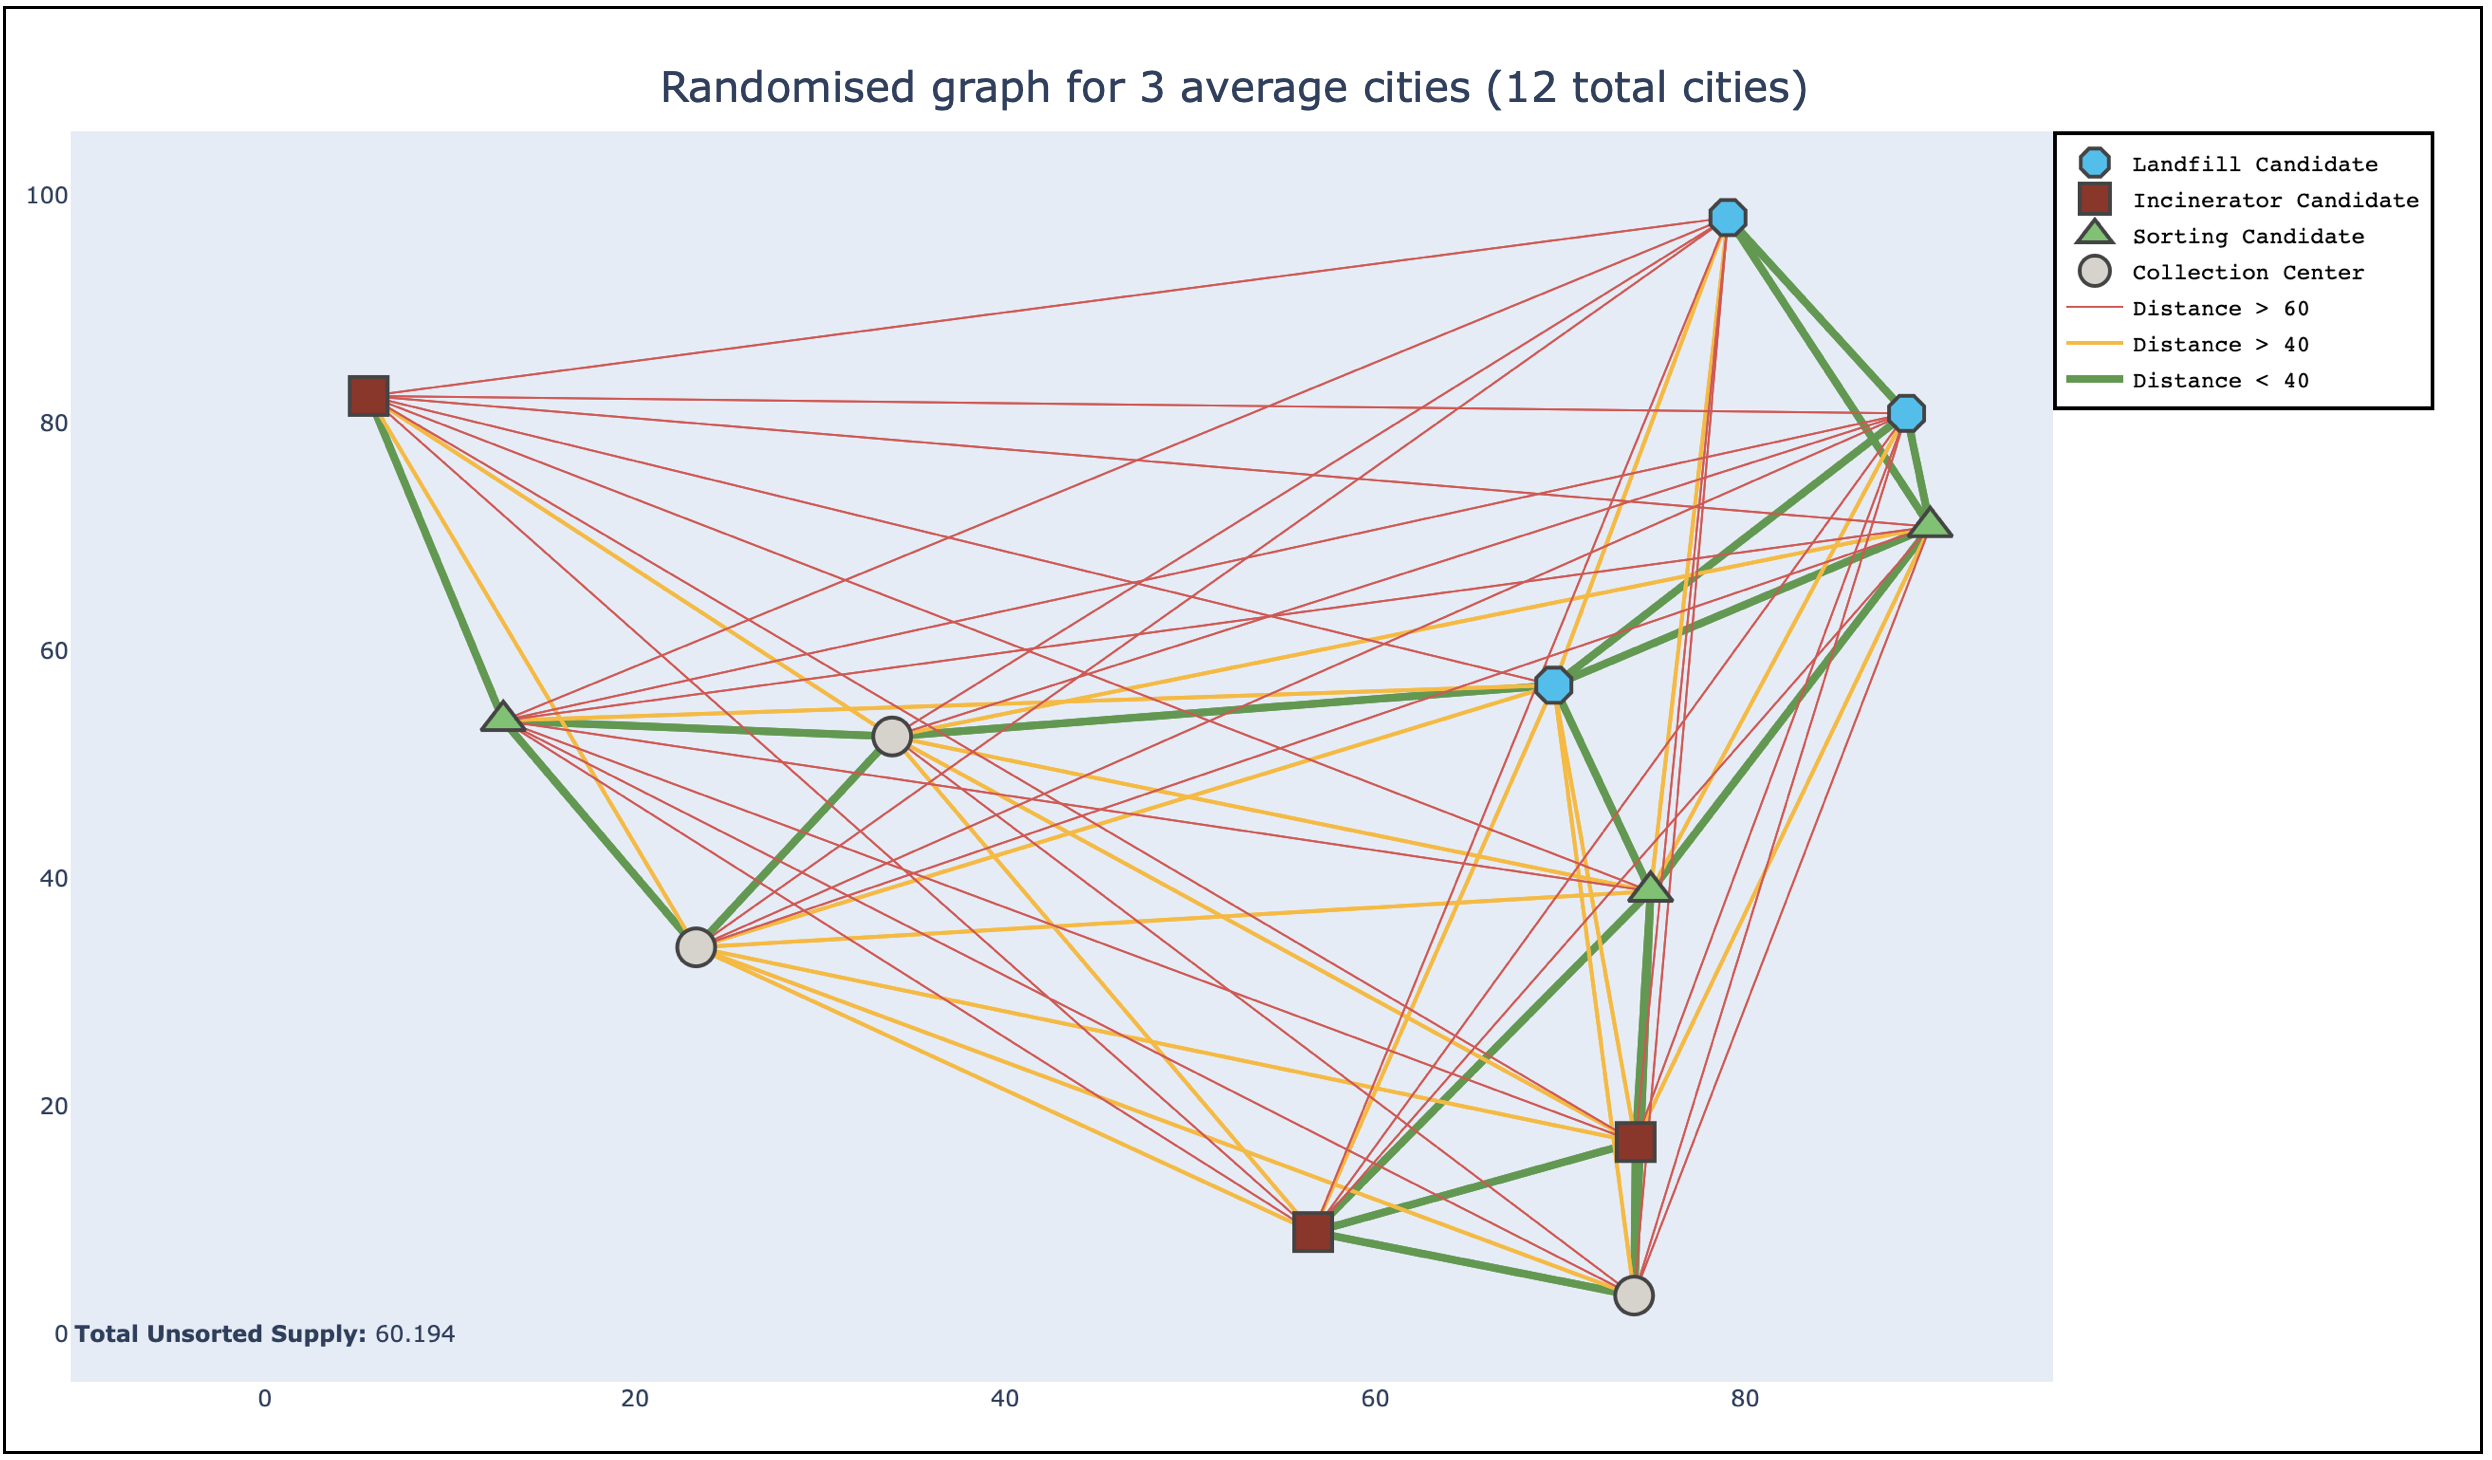
\includegraphics[width=\linewidth]{/methodology/3_cities_randomised.png}
    \caption{Graph generation with three number of average cities, 12 total cities.}
    \label{fig:3_city_graph}
\end{figure}
\begin{figure}[ht]
    \centering
    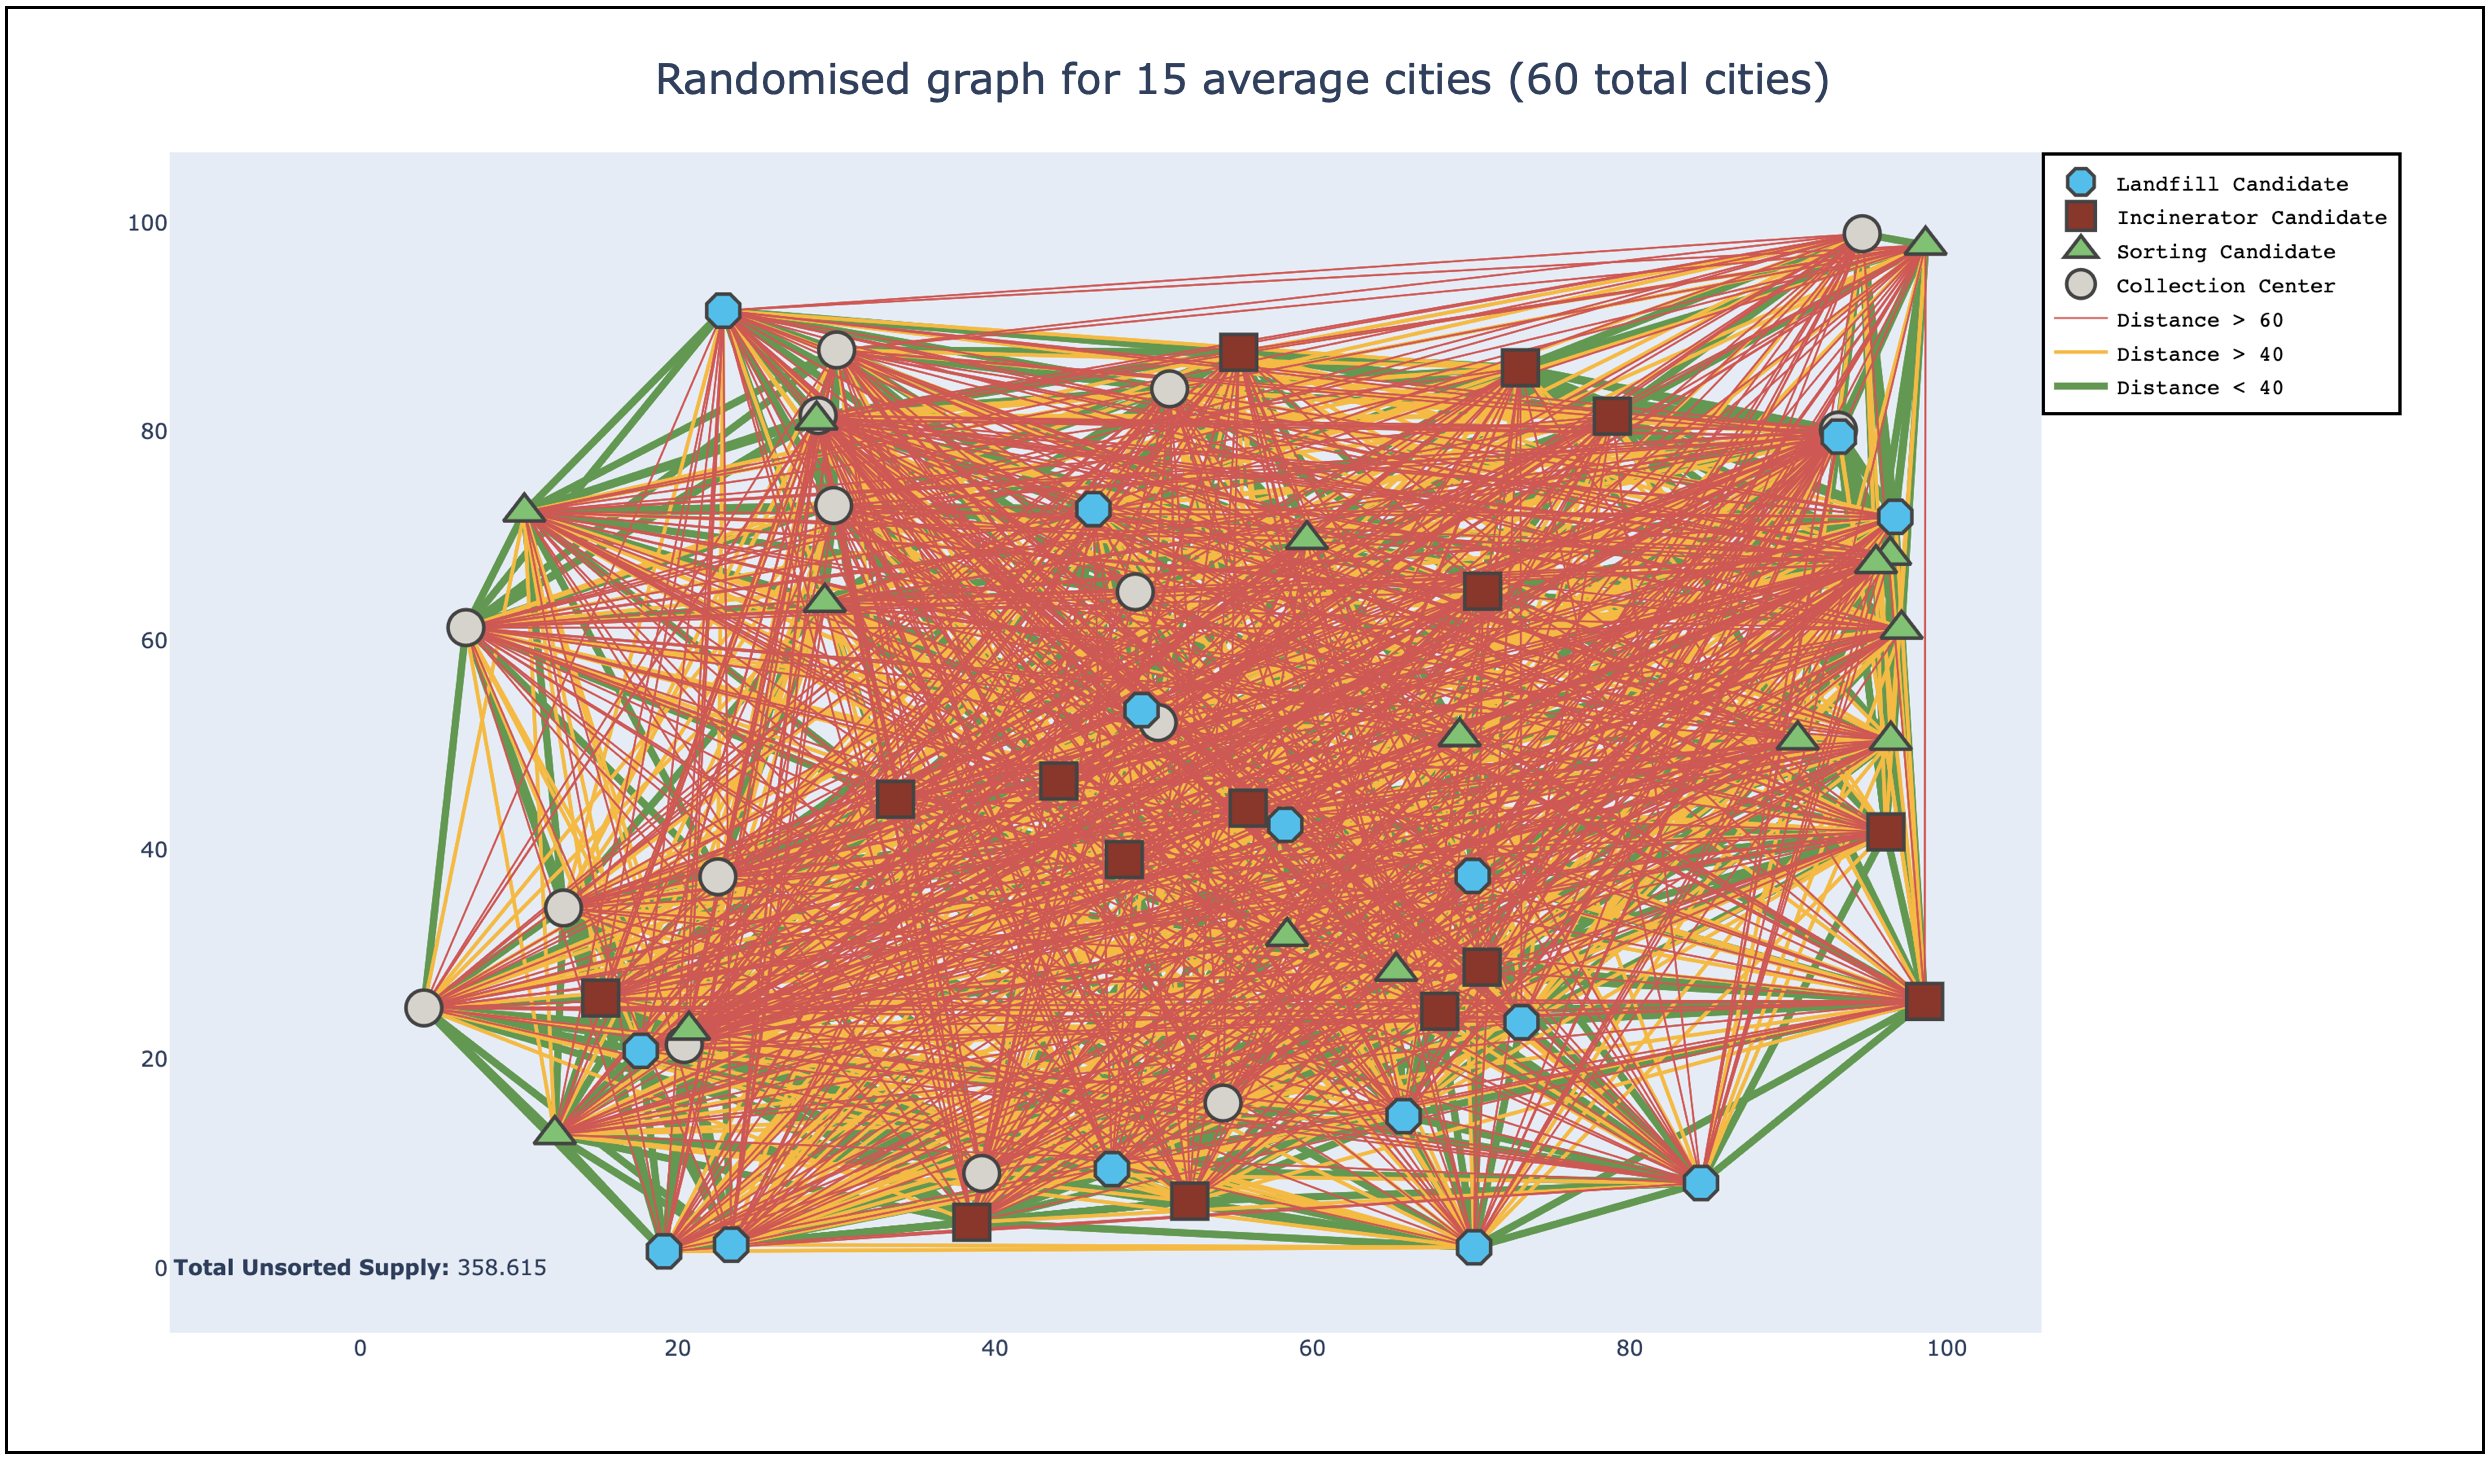
\includegraphics[width=\linewidth]{/methodology/15_city_randomised.png}
    \caption{Graph generation with 15 number of average cities, 60 total cities.}
    \label{fig:15_city_graph}
\end{figure}
\clearpage
\section{Conclusion}
In this chapter, we started by showing the data gathering procedure by looking into the case study of Pathum Thani by \cite{olapiriyakul_multiobjective_2019} and using the health impact, land usage, facility and vehicle capacity data. Moreover, we showed data gathered from real-life sources and research papers on the construction cost of incinerators and landfill facilities. Additionally, we displayed the cost of the sorting facilities, as there were no reputable sources for the construction cost of these facilities. 
Afterwards, we conveyed the method for the evolutionary algorithms, where we adapted the crossover and mutation operators to obtain solutions that are in the feasible regions of the problem and that have a reduced number of active facilities. Finally, we presented the graph generation procedure, which includes the generation of random graphs used to confirm the claims made throughout this Thesis.

\chapter[Implementation]{Implementation}\label{chapter:implementation}
This section covers the implementation approaches of the initially proposed MILP model by \cite{olapiriyakul_multiobjective_2019} with CPLEX 20.1.0 and the problems and solutions to the evolutionary algorithm implementation using the Pymoo multi-objective optimisation library by \cite{blank_pymoo_2020}. Finally, we give insight into the parameter choices of the various algorithms and show the Hypervolume performance indicator to measure the algorithms' performance.
\section{Exact solution optimisation}
As illustrated in the original paper proposed by \cite{olapiriyakul_multiobjective_2019}, we use the CPLEX optimisation framework as an exact solution approach to single objective problems and an approximate solution approach for bi-objective and multi-objective problems. The CPLEX framework solves linear programming problems, mixed-integer linear programming problems, and quadratic objective problems. If the objective is a linear or convex quadratic function, CPLEX can solve them. The CPLEX callable library is written in C and allows for embedding into Python as it can call C functions for easier use by the programmer. We use this library as a baseline for the approach by \cite{olapiriyakul_multiobjective_2019} as it is state-of-the-art for optimising linear programs. 
\\\\
Figures \ref{fig:single_cplex_three_cities} and \ref{fig:multi_cplex_three_cities} show the CPLEX solutions to the problem in figure \ref{fig:3_city_graph}. As shown by \cite{olapiriyakul_multiobjective_2019}, we obtain the single objective solutions and then solve for the bi-objective and the three objective problem formulations. As this approach only gives a single best solution for each problem formulation, we will always receive seven solutions for every problem.
\begin{figure}[ht]
    \centering
    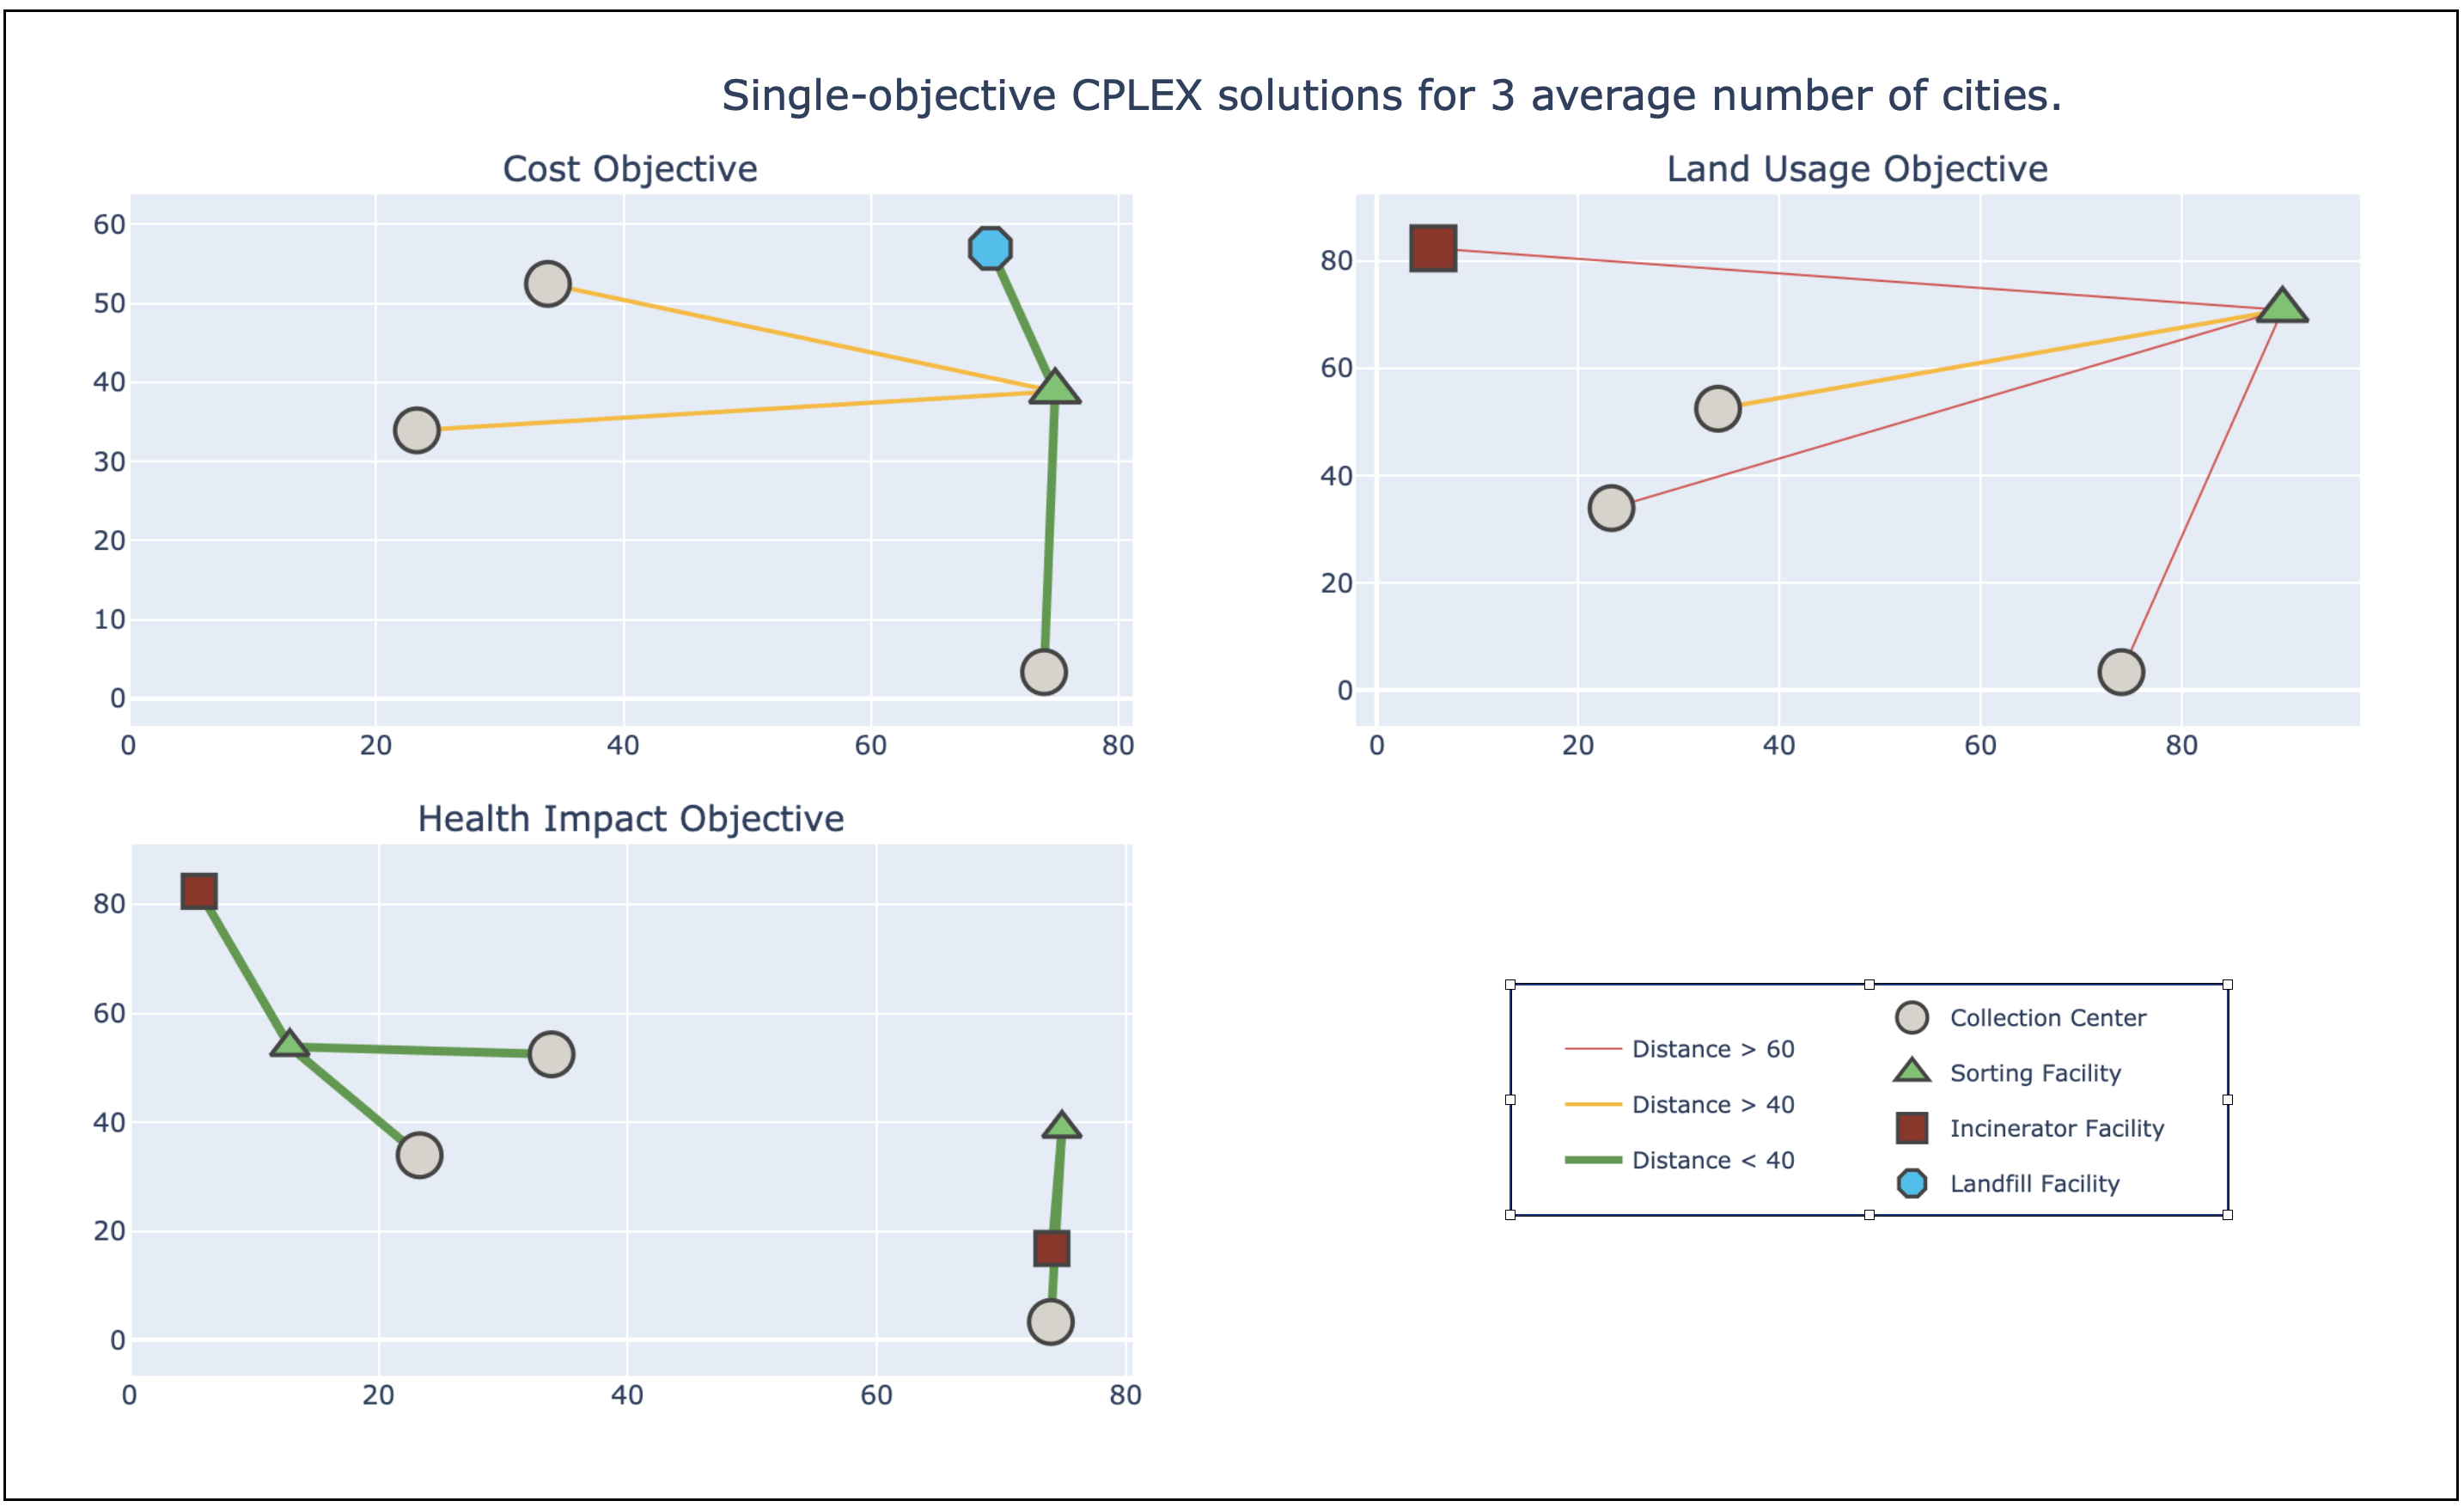
\includegraphics[width=\linewidth]{/implementation/singleobj_CPLEX_3_cities.png}
    \caption{Single objective solution with CPLEX for three average cities.}
    \label{fig:single_cplex_three_cities}
\end{figure}
\begin{figure}[ht]
    \centering
    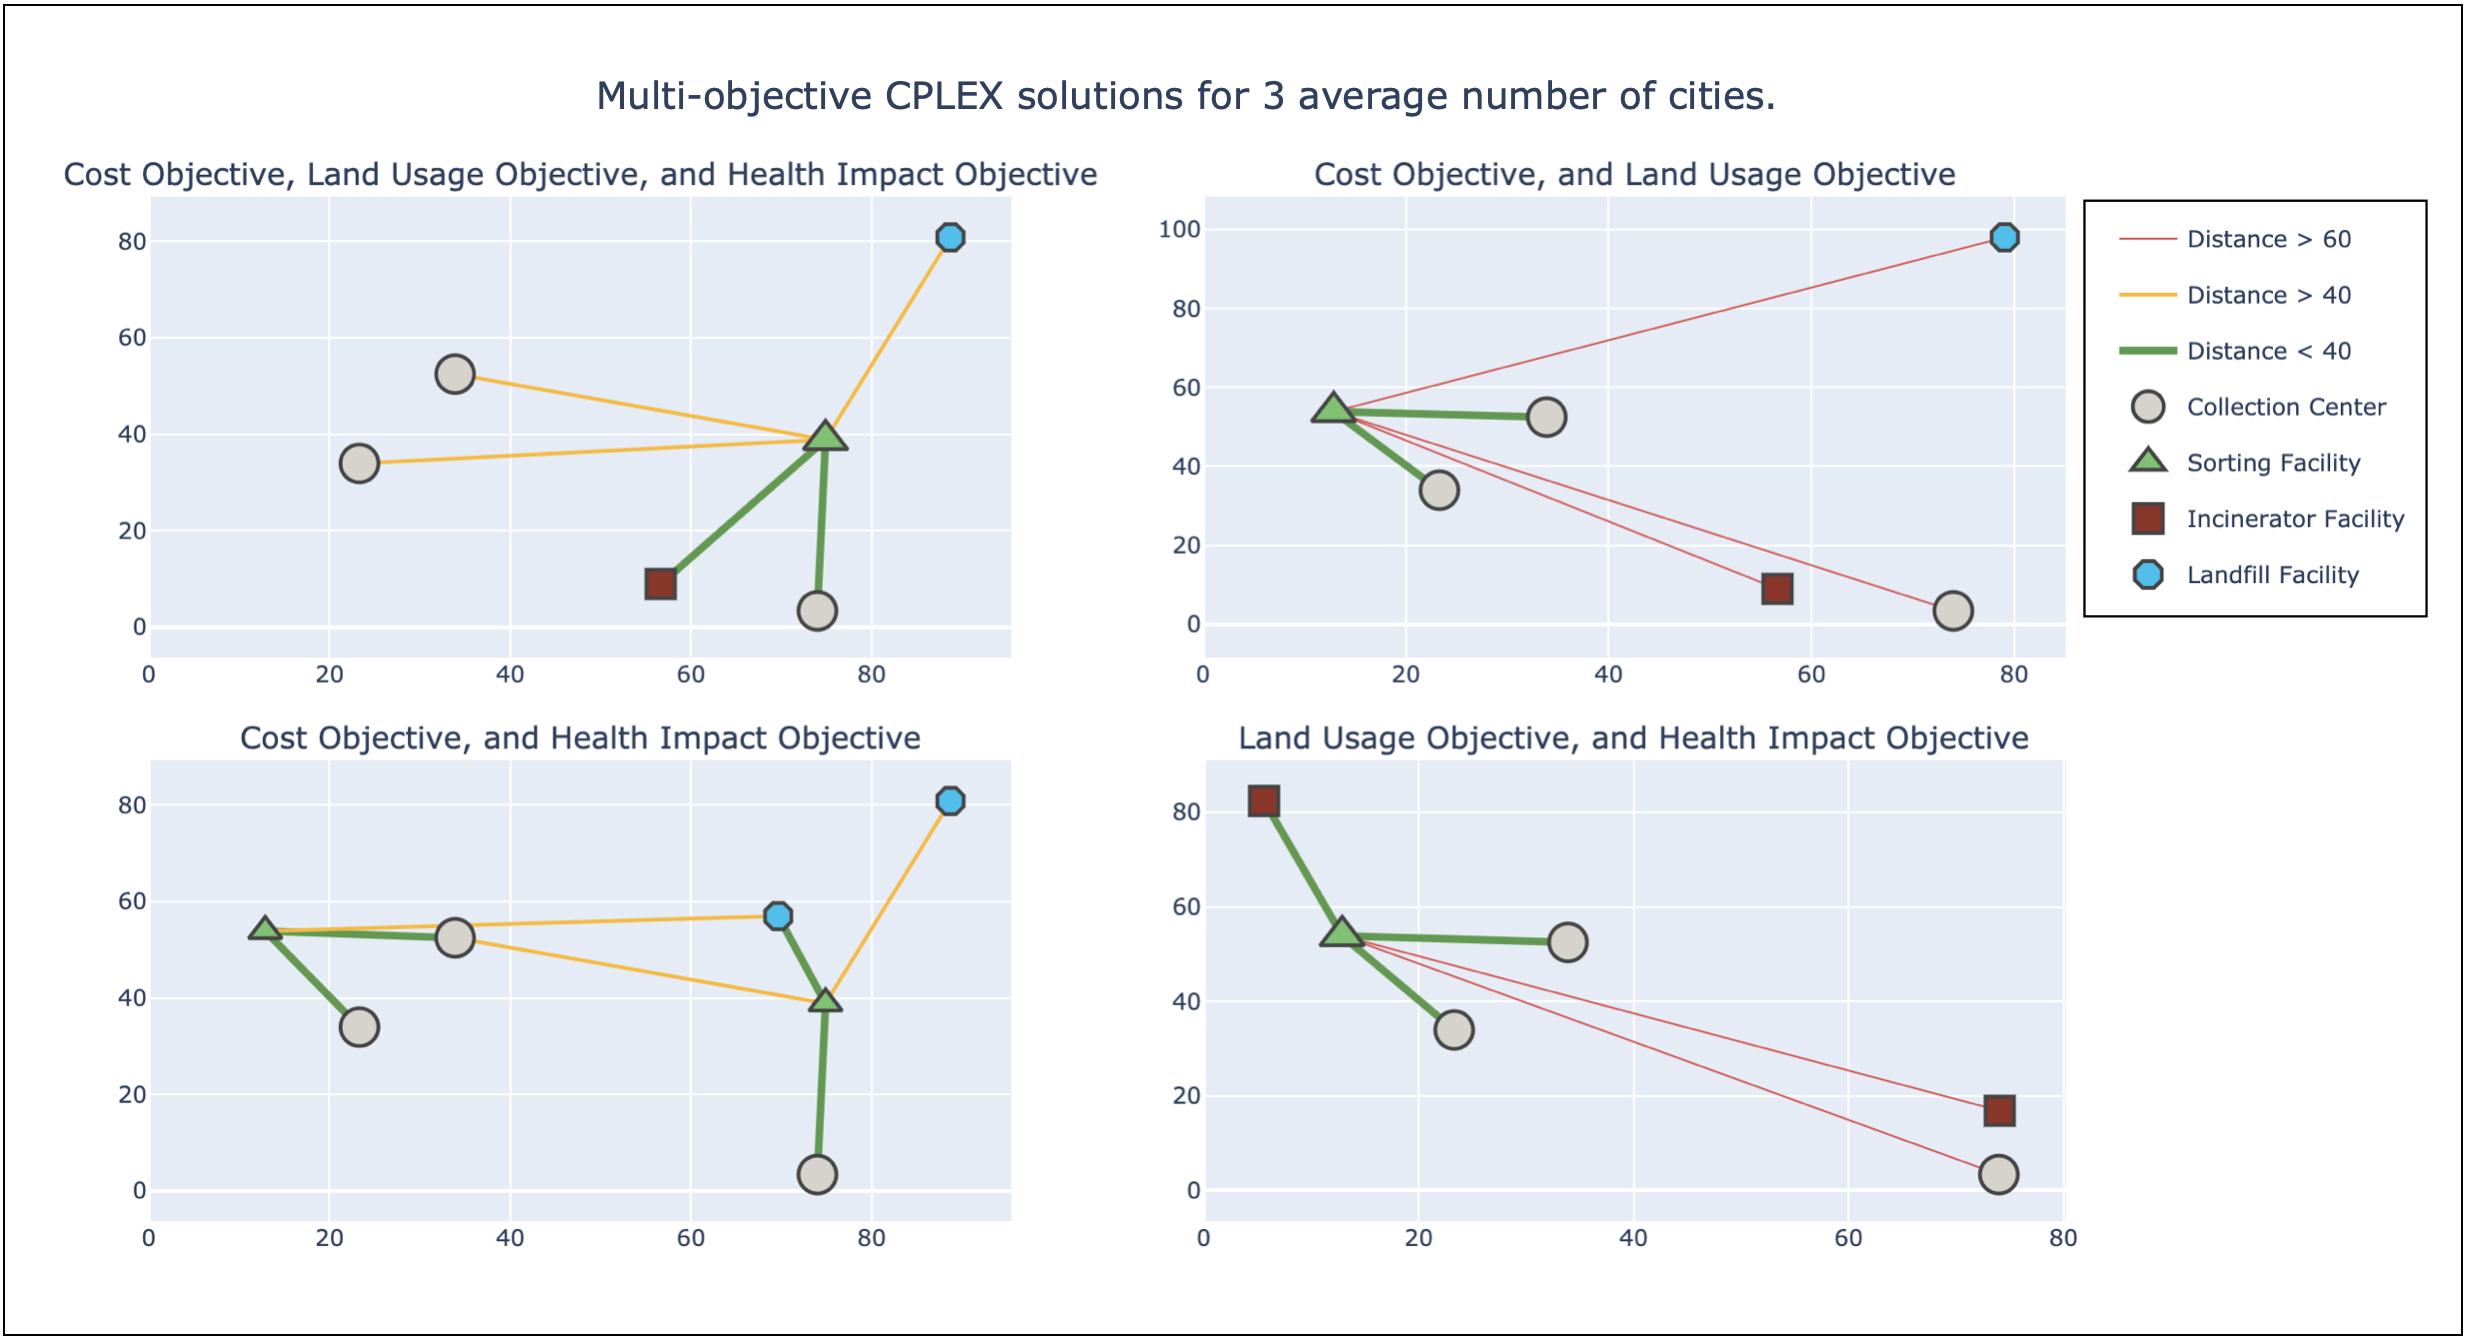
\includegraphics[width=\linewidth]{/implementation/multiobj_CPLEX_3_cities.png}
    \caption{Multi-objective solution with CPLEX for three average cities.}
    \label{fig:multi_cplex_three_cities}
\end{figure}
\clearpage
\section{Evolutionary Algorithms}
We use the Pymoo framework (version 0.5.0), \cite{blank_pymoo_2020}, for the evolutionary optimisation, which allows for a straightforward implementation of the constrained MILP problem by \cite{olapiriyakul_multiobjective_2019}. Furthermore, it allows for a fast implementation of multiple evolutionary algorithms. We start by implementing the problem and its constraints in a vectorised form, allowing for a faster execution time. Furthermore, we set the upper bound of the integer decision variables, $x$, and real numbered decision variables, $f$, to equations \ref{eq:x_ub} and \ref{eq:f_ub}, respectively. 
\begin{alignat}{2}
    x_{ub} &= \left\lceil \frac{\sum_{i \in I} D_i}{\overline{C}_{ij}}  \right\rceil, \quad \forall j \in J \label{eq:x_ub}\\
    f_{ub} &= \sum_{i \in I} D_i\label{eq:f_ub}
\end{alignat}
    
The lower bound for all decision variables is zero. In the worst case, we allow for the transportation of the total supply on a single link from a sorting facility to a landfill or incinerator.
The original vectorised implementation contained three significant problems:
\begin{enumerate}
    \item It was finding a minimal amount of solutions that are in the feasible region.
    \item It was slow at finding the feasible region of the solution space.
    \item The feasible solutions found used all available sorting, incinerator, and landfill candidate facilities, which induces very high objective costs.
\end{enumerate}
For the first problem, instead of prioritising selecting feasible solutions, we added a penalty of $10^8$ multiplied by the amount of constraint violation to the objective functions and, as such, found more solutions, even if they were infeasible. The next goal was to move into the feasible region faster. To move into the feasible region faster, we added the real numbered crossover and mutation operators found in the methodology in section \ref{sec:real_dec_variables}. For the base mutation, we use a polynomial mutation which uses the same probability distribution found in \cite{deb_self-adaptive_2007}, where $u_i$ is a random number between $0$ and $1$.
\begin{equation}\label{eq:sbx_prob}
    \mathcal{P}(\beta_{qi}) = 
    \begin{cases}
        (2 u_i + (1 - 2 u_i)(1-\beta_{(1, i)}^{\eta_c}))^{1/\eta_c} - 1, \quad &\textit{if} \: u_i \leq 0.5; \\
        1 - (2 (1 - u_i) + 2 (u_i - 0.5) \beta_{(2, i)}^{\eta_c})^{1/\eta_c}, \quad &\textit{otherwise}.
    \end{cases}
\end{equation}
The spread factor $\beta_i$ is the ratio of the absolute difference in selected mutation values to that of the upper bound and lower bound.
\begin{alignat}{2}
    \beta_{(1,\: i)} &= \left | \cfrac{x_i^t - x_{lb}}{x_{ub} - x_{lb}}\right| \\
     \beta_{(2, \: i)} &= \left| \cfrac{x_i^t - x_{ub}}{x_{ub} - x_{lb}}\right|
\end{alignat}
The distribution index $\eta_c$ is any non-negative real number. A large value of $\eta_c$ gives a higher probability of creating values closer to the non-mutated values. In contrast, a small value of $\eta_c$ allows the creation of distant values to the non-mutated values.
\\
After obtaining $\beta_{qi}$ from equation \ref{eq:sbx_prob} the calculation of the new mutated values is as follows:
\begin{equation}
    x_i^{t+1} = x_i^t + (x_{ub} - x_{lb})\beta_{qi}
\end{equation}
This probability distribution helps us create new values similar to the old ones.
Both of these operators allowed us to meet the hard constraints of the problem that required to be precisely equal to each other. These allowed us to obtain feasible solutions; however, these still used all available sorting, incinerator, and landfill candidate facilities.
\\\\
In order to cancel out redundant facilities, we apply the repair operator outlined at the end of section \ref{sec:real_dec_variables}, which allows searching for facility cancellations while staying in the feasible region of the search space. 
\\
Furthermore, the introduction of zeroes produced a division by zero for the normalisation of the incinerator and landfill values, as there was no supply flowing into some sorting centres. To fix these issues, in the adapted crossover and mutation, we set the row of the sorting facility with zero supply flow to the incinerators K and landfills K' to zero. We also set the flow supply of the sorting facility with zero supply flow to one to create a division of one. Algorithm \ref{alg:updated_norm} delineates the updated normalisation procedure.
\begin{algorithm}[ht]
    \caption{Updated normalisation procedure}\label{alg:updated_norm}
    $S \gets \sum_{i \in I} f_{ij}, \quad \forall j \in J$;\\
    \For{$j \in J$}{  
        \For{$k \in K \cup K'$}{
            \If{$S_j = 0$}{
                $f_{jk} \gets 0$;
            }}
        $S_j \gets 1$;    
    }
    Apply Normalisation:\\
    \For{$j \in J$}{
        \For{$k \in K \cup K'$}{
            $f^n_{jk} \gets \gets \cfrac{f_{jk}}{S_j}$;
        }
    }
\end{algorithm} 
\\\\
This approach gave satisfactory results for smaller problems; however, there was a violation of the binary constraints \ref{one_size_j} -- \ref{one_size_k_prime}  on large-scale problems. These violations had multiple reasons,
\begin{enumerate}
    \item There needed to be a higher number of facilities open in order to satisfy the amount of supply.
    \item The standard crossover and mutation operators introduce multiple sizes into the solution space without removing the old sizes.
\end{enumerate}
For these reasons, we decided to adapt the binary crossover and mutation to the one proposed in section \ref{sec:bin_dec_var}. 
\\\\
In order to find the most performant algorithm without knowing the Pareto front, we use the hypervolume indicator first proposed by \cite{hutchison_indicator-based_2004}. The hypervolume indicator indicates the quality of a non-dominated set. It does this by using a reference point, usually set to one, after normalising the objectives using the nadir and ideal points, i.e. the worst and best points found, respectively. The goal of the hypervolume is to maximise the dominated area, as this means that the points are closer to the ideal point. Figure \ref{fig:hv_indicator} shows an example of the hypervolume indicator, adapted from \cite{fonseca_improved_2006}. It illustrates a dual objective case with three points where the dominated area is grey.
\\\\
We use a tolerance on the objective space for the termination criterion to terminate once we reach a converged state. It calculates the change from the last ideal and nadir points to the current ideal and nadir points. The parameters include a sliding window that checks the last $\gamma$ points at every iteration $t$, a maximum amount of generations, $g$, and a tolerance value, $f_{tol}$, that stops the algorithm if there has not been a significant change between the last and current ideal and nadir points.\\\\
Tables \ref{tab:evo-params} and \ref{tab:term-criterion_params} summarise the parameters used for the evolutionary algorithm and the termination criterion for large and small-scale problems. We decrease the mutation probability for the evolutionary algorithm to reduce the exploration of the vast search space. Furthermore, we use the Riesz s-energy approach (Section \ref{ref_points}) for the reference points implemented in Pymoo from \cite{blank_generating_2021}. We use this approach as we want a solution for each population member on each reference point to maximise the number of solutions.
\\\\\\
Figures \ref{fig:evo_3_cities} and \ref{fig:evo_15_cities} show the best solutions of the evolutionary algorithms for three and 15 cities, respectively, based on the hypervolume of the ideal points, which are the single objective solutions found by CPLEX, and the nadir points, which are the worst points found by all algorithms. 
For figure \ref{fig:evo_3_cities} we see quite the difference in solutions compared with the previous solution found by using the min-max approach with CPLEX in figure \ref{fig:multi_cplex_three_cities}. Furthermore, in figure \ref{fig:evo_15_cities}, we see the use of more sizes than in the previous figures. We use large, medium, and small facilities for incinerators and sorting facilities. We only use medium and small facilities across the algorithms for the landfill facilities.
\begin{table}[ht]
\centering
\resizebox{\textwidth}{!}{%
\begin{tabular}{@{}lcccc@{}}
\toprule
\multicolumn{5}{c}{\textbf{Evolutionary algorithm parameters}} \\ \midrule
\multicolumn{1}{c}{\textit{Problem size}} & \multicolumn{1}{l}{\textit{Population size}} & \multicolumn{1}{l}{\textit{Reference points}} & \multicolumn{1}{l}{\textit{Crossover probability}} & \multicolumn{1}{l}{\textit{Mutation probability}} \\
Small scale ($\leq 10$) & $200$ & $200$ & $80 \%$ & $1 \%$ \\
Large scale ($> 10$) & $200$ & $200$ & $80 \%$ & $0.5 \%$ \\ \bottomrule
\end{tabular}%
}
\caption{Parameters used for the evolutionary algorithms, for large and small scale problems.}
\label{tab:evo-params}
\end{table}


\begin{table}[ht]
\centering
\resizebox{\textwidth}{!}{%
\begin{tabular}{@{}ccccc@{}}
\toprule
\multicolumn{5}{c}{\textbf{Termination criterion parameters}} \\ \midrule
\textit{Problem size} & \textit{Termination tolerance ($f_{tol}$)} & \textit{Sliding window amount ($\gamma$)} & \textit{Sliding window iteration ($t$)} & \textit{Maximum amount of generations ($g$)} \\
Small scale ($\leq 10$) & $0.01$ & $30$ & $5$ & $1000$ \\
Large scale ($> 10$) & $0.01$ & $30$ & $5$ & $1000$ \\ \bottomrule
\end{tabular}%
}
\caption{Parameters used for the termination criterion, for small scale and large scale problems.}
\label{tab:term-criterion_params}
\end{table}
\begin{figure}[ht]
    \centering
    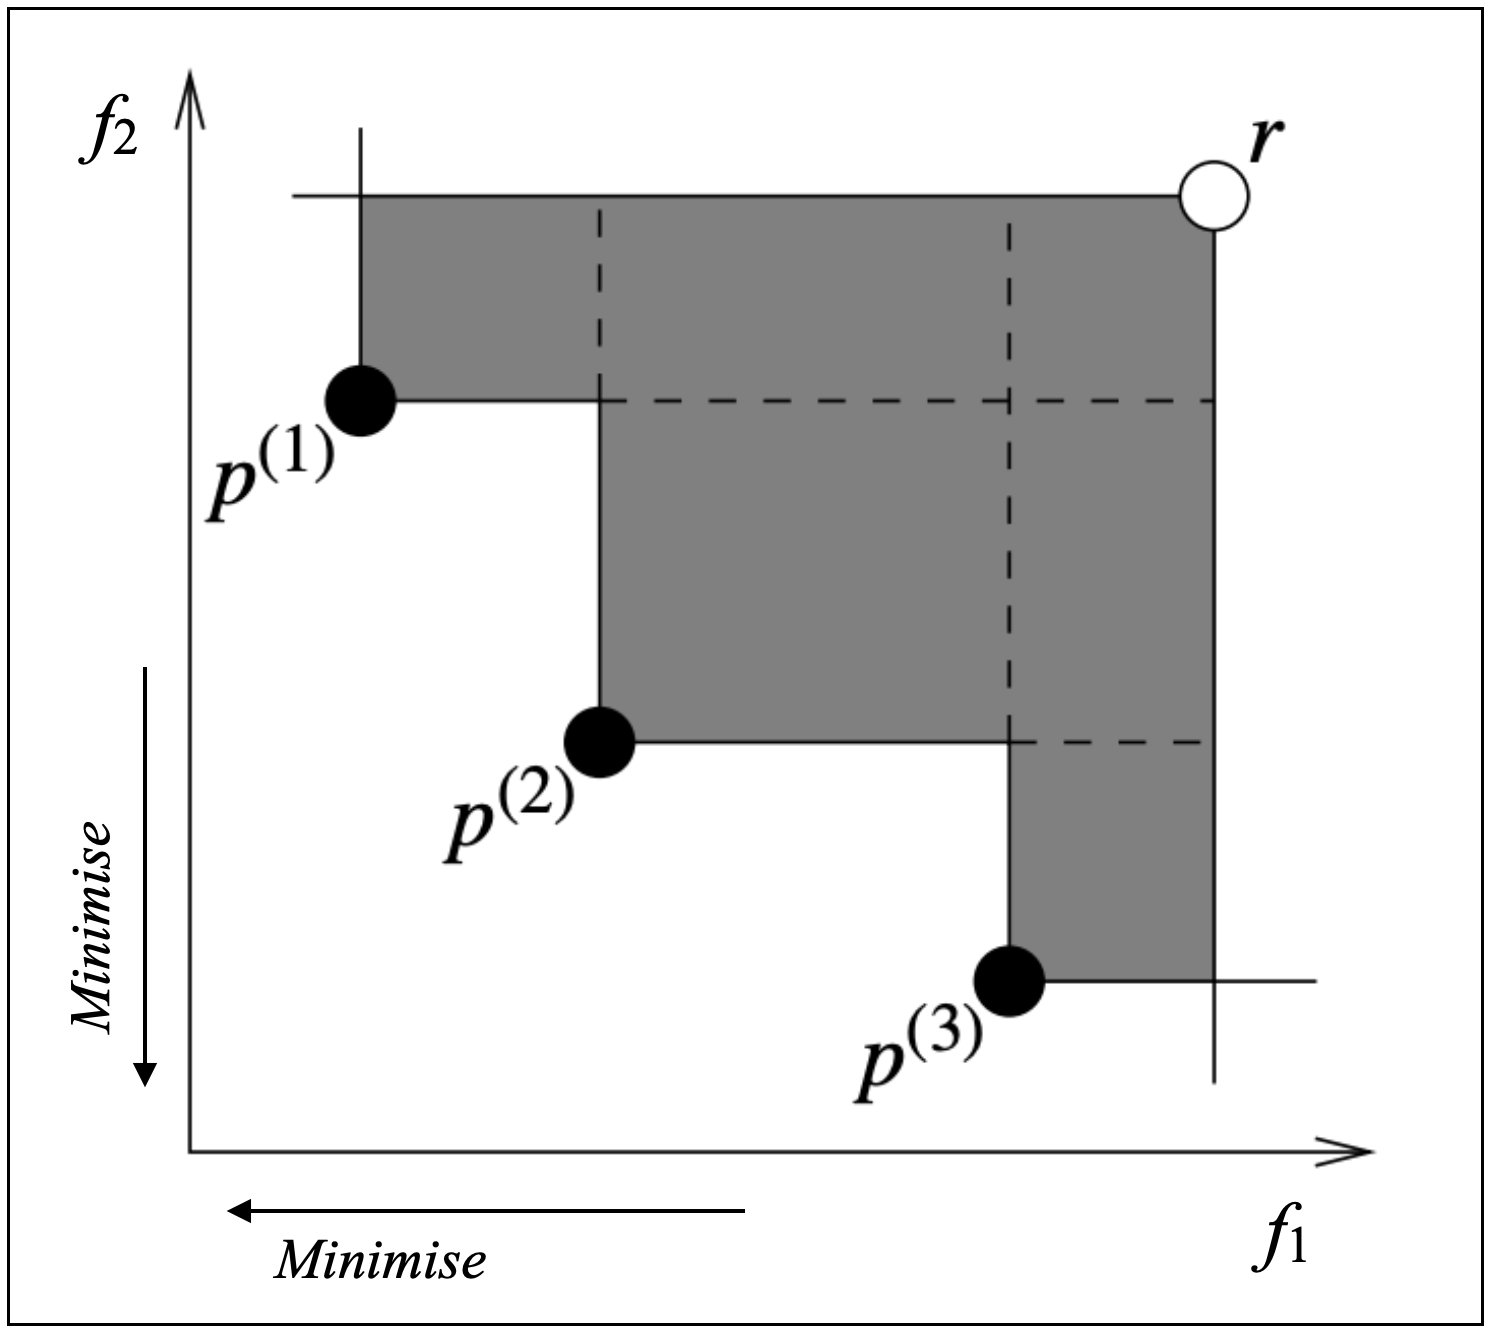
\includegraphics[scale=0.3]{/implementation/hypervolume_indicator.png}
    \caption{The hypervolume indicator shown for a dual objective problem.}
    \label{fig:hv_indicator}
\end{figure}
\begin{figure}
    \centering
    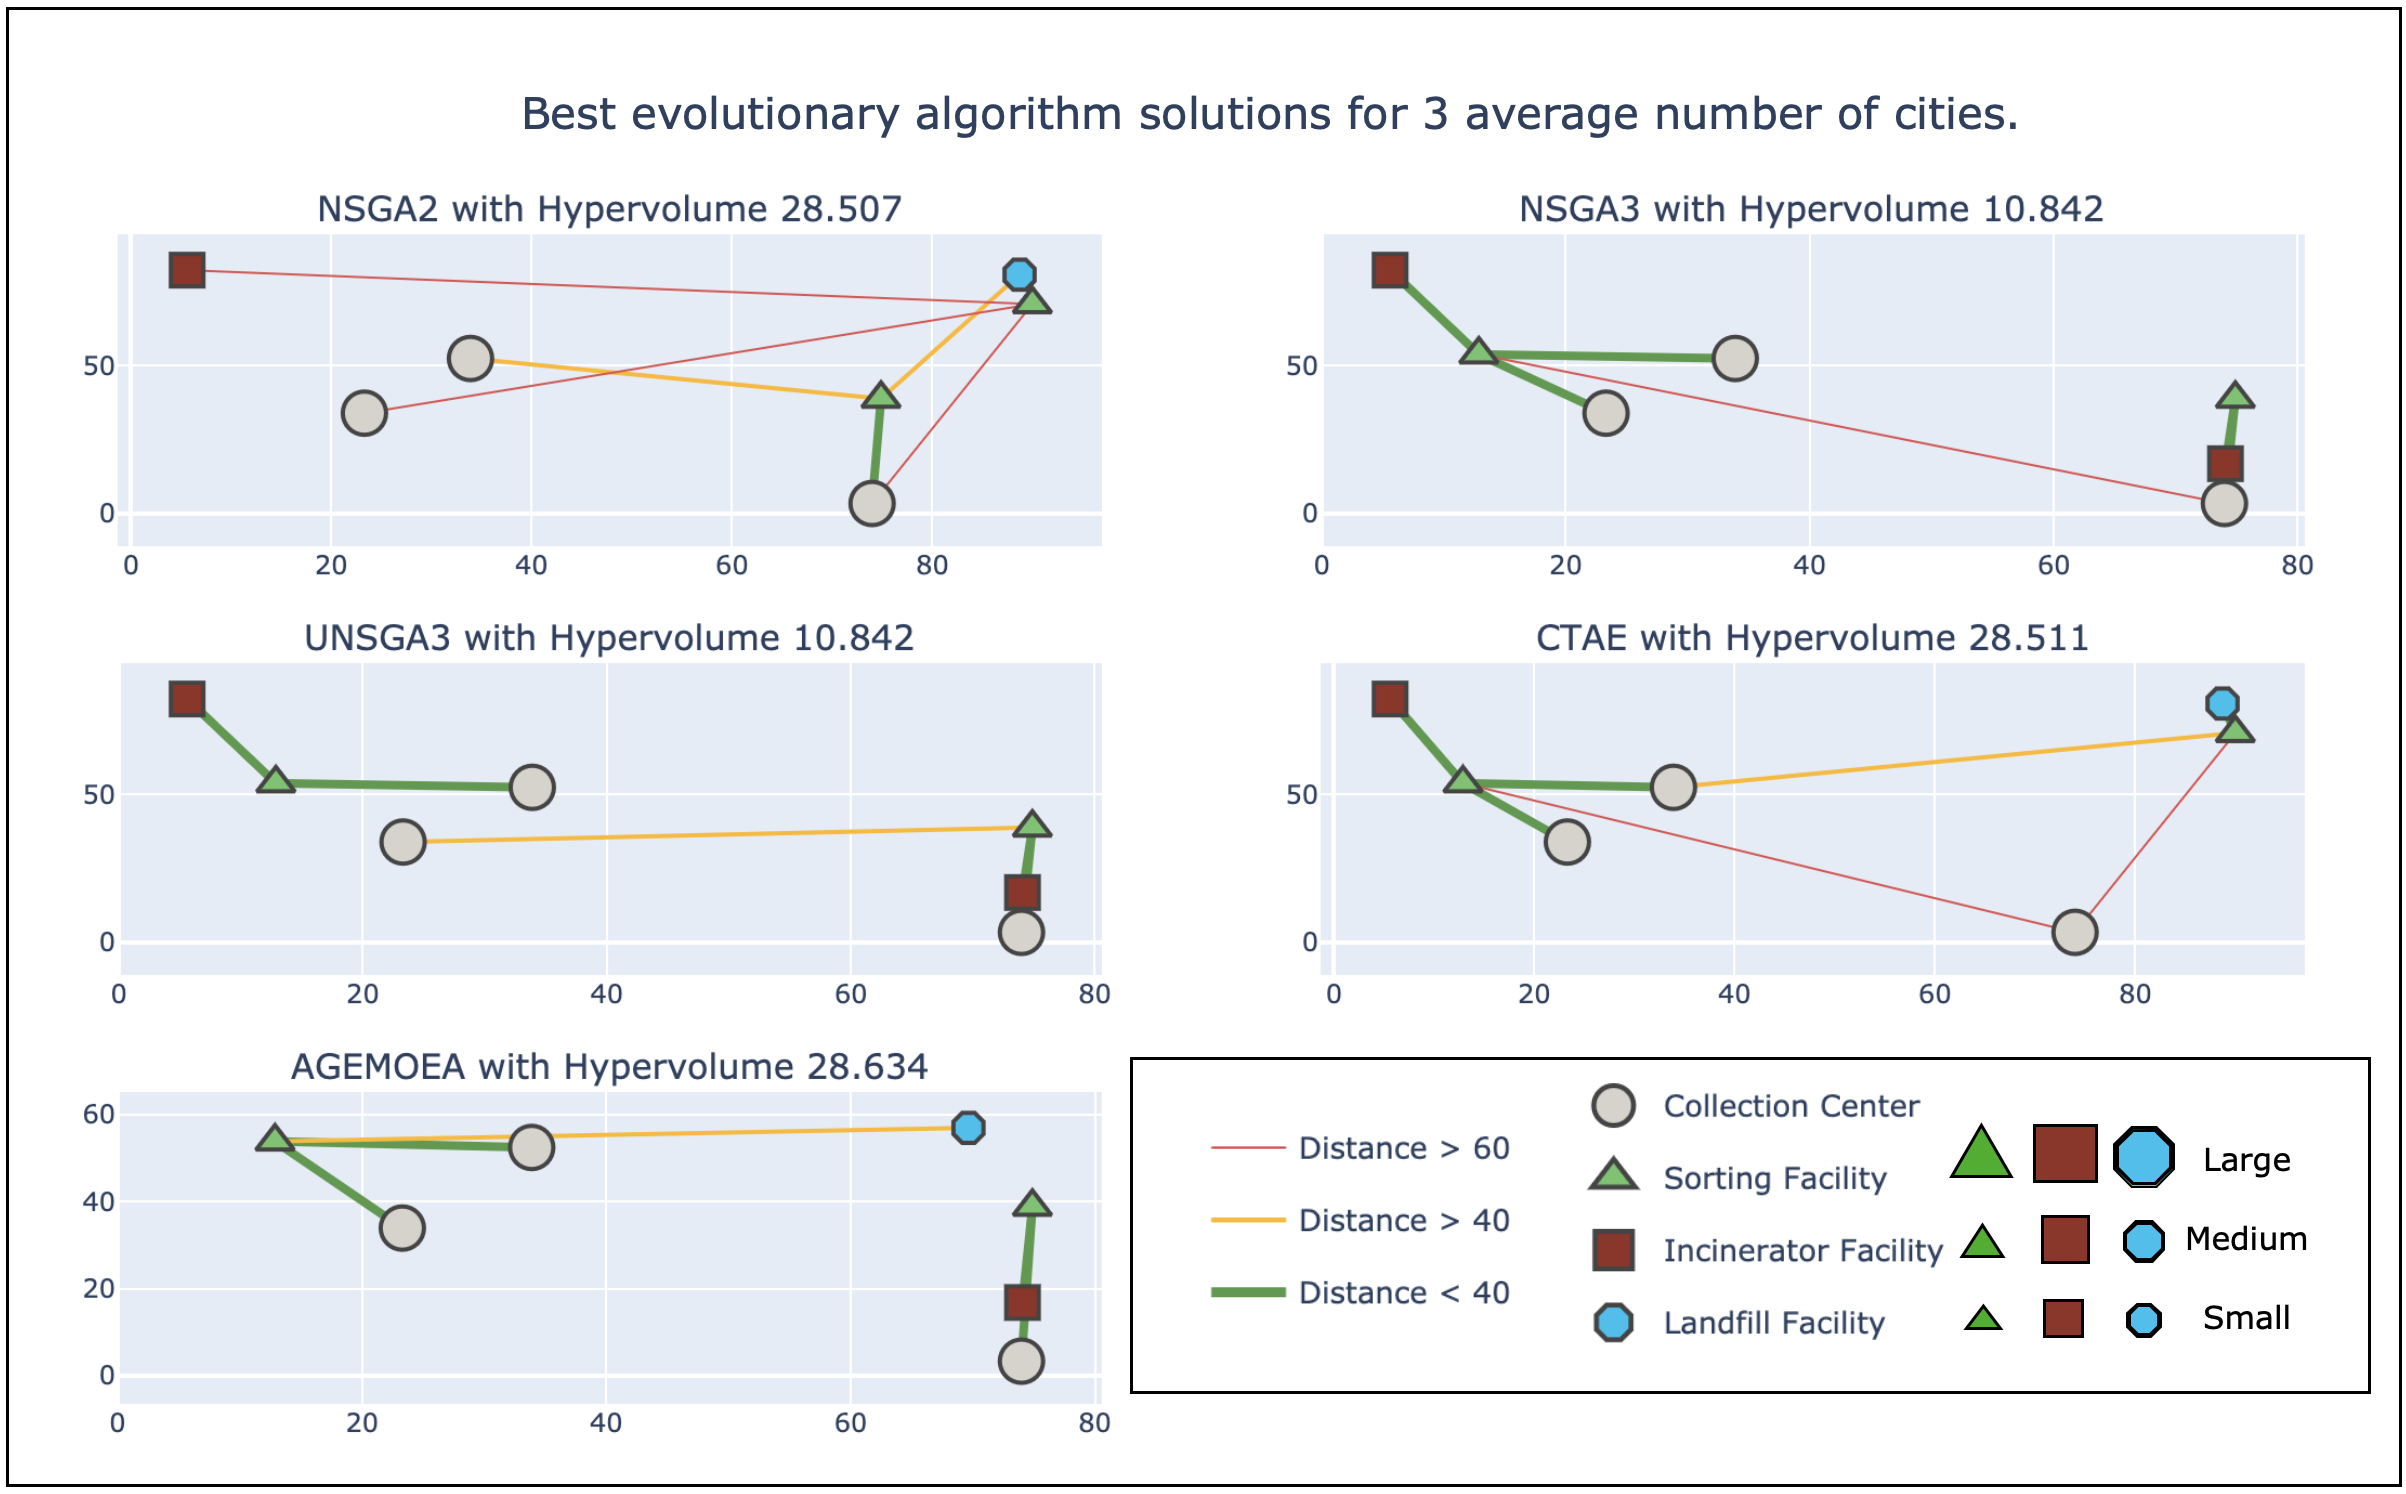
\includegraphics[width=\textwidth]{/implementation/evo_3_cities.png}
    \caption{Evolutionary algorithm solutions for three cities.}
    \label{fig:evo_3_cities}
\end{figure}
\begin{figure}
    \centering
    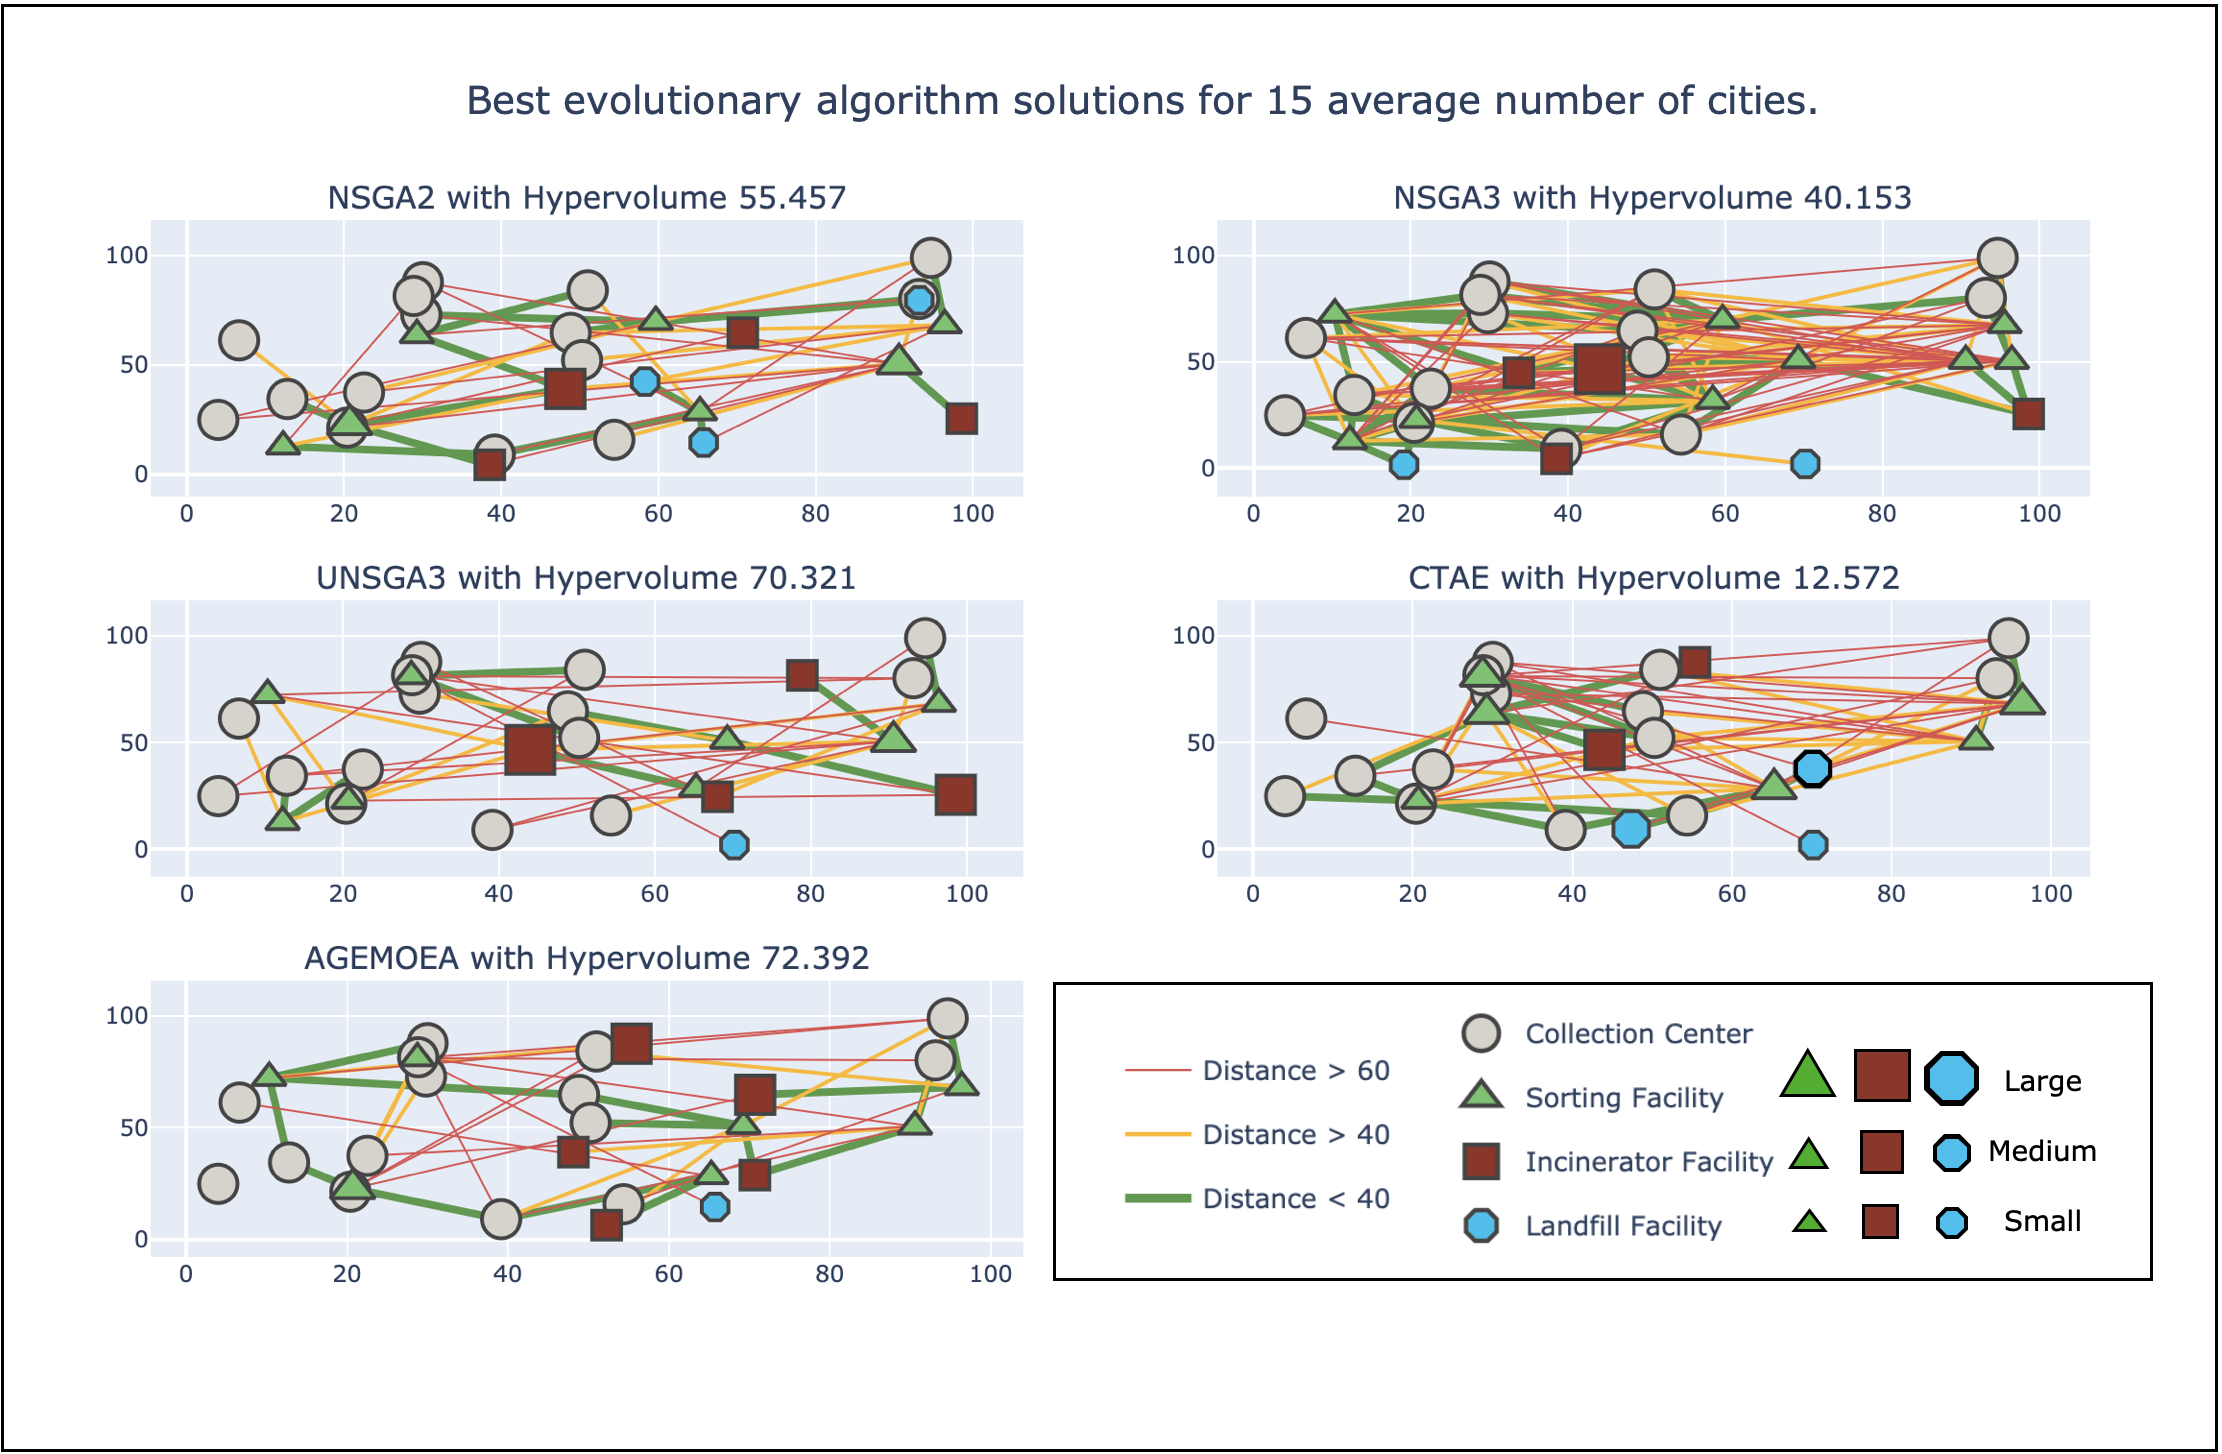
\includegraphics[width=\textwidth]{/implementation/evo_15_cities.png}
    \caption{Evolutionary algorithm solutions for 15 cities.}
    \label{fig:evo_15_cities}
\end{figure}
\clearpage
\section{Conclusion}
In this chapter, we illustrated the implementation of the branch and cut algorithm using the CPLEX algorithm and provided an example of a solution to the randomised graph generated in section \ref{sec:graph_generation}. Furthermore, we gave insight into the evolutionary algorithms' implementation, calculating the upper and lower bound for the integer and continuous variables, $x$ and $f$, respectively. Moreover, we showed the updated normalisation to handle division by zero cases. Finally, we gave the evolutionary algorithms' parameter choices, providing the population amount, reference point amount, crossover probability, and mutation probability. We also gave insight into the hypervolume performance measure to find the difference between the solutions without providing a Pareto front.
\chapter[Empirical Study]{Empirical Study}\label{chapter:results}
This chapter presents the results obtained to validate the claims made throughout this Thesis. The claims we made in this Thesis included:

\begin{enumerate}
    \item We are decreasing the time needed to solve large-scale multi-objective MILP problems in waste management.
    \item We are obtaining reasonable solutions close to the CPLEX MILP model.
    \item We are creating trade-offs over the three objectives by obtaining a Pareto set of diverse solutions.
\end{enumerate}
We ran the experiments with the CPLEX and evolutionary algorithms on two to ten average numbers of cities, with ten randomised graphs per average city and three seeds per graph. We then went from 15 to 30 average number of cities and a final experiment on 40 average number of cities. For these, we only used the evolutionary algorithms and the same graph construction count with three seeds. In total, we ran $2370$ experiments, with $1620$ being the experiments from two cities to ten cities and $750$ being the experiments from 15 cities to 30 cities and 40 cities.
\\\\
We calculated the hypervolume percentage for each multi-objective solution using the ideal points from the CPLEX solutions for the small-sized problems and the ideal points from the evolutionary algorithm solutions for the large-sized problems. Moreover, we calculated the nadir points for both approaches as the worst points obtained in that run. Table \ref{tab:experiment_const} shows a summarisation of the construction of experiments.


\begin{table}[ht]
\centering
\resizebox{\textwidth}{!}{%
\begin{tabular}{@{}ccccc@{}}
\toprule
\multicolumn{5}{c}{\textbf{Experiment construction}} \\ \midrule
\multicolumn{1}{l}{\textit{Number of average cities}} & \textit{Algorithms} & \multicolumn{1}{l}{\textit{Number of generated random graphs}} & \textit{Seeds} & \multicolumn{1}{l}{Total number of experiments} \\
$2$ & CPLEX and Evolution & $10$ & $3$ & $180$ \\
$3$ & CPLEX and Evolution & $10$ & $3$ & $180$ \\
$4$ & CPLEX and Evolution & $10$ & $3$ & $180$ \\
$5$ & CPLEX and Evolution & $10$ & $3$ & $180$ \\
$6$ & CPLEX and Evolution & $10$ & $3$ & $180$ \\
$7$ & CPLEX and Evolution & $10$ & $3$ & $180$ \\
$8$ & CPLEX and Evolution & $10$ & $3$ & $180$ \\
$9$ & CPLEX and Evolution & $10$ & $3$ & $180$ \\
$10$ & CPLEX and Evolution & $10$ & $3$ & $180$ \\
$15$ & Evolution & $10$ & $3$ & $150$ \\
$20$ & Evolution & $10$ & $3$ & $150$ \\
$25$ & Evolution & $10$ & $3$ & $150$ \\
$30$ & Evolution & $10$ & $3$ & $150$ \\
$40$ & Evolution & $10$ & $3$ & $150$ \\
\multicolumn{1}{l}{} & \multicolumn{1}{l}{} & \multicolumn{1}{l}{} & \multicolumn{1}{l}{} & \textbf{Total: $\mathbf{2370}$} \\ \bottomrule
\end{tabular}%
}
\caption{Construction of the experiments for the empirical study.}
\label{tab:experiment_const}
\end{table}
\clearpage
\section{Time observations}\label{sec:time_res}
Figure \ref{fig:log_time} shows the average time for the CPLEX optimiser (Branch and cut) and the evolutionary algorithms described in \ref{sec:nsga2} -- \ref{sec:agemoea} (NSGA-II, NSGA-III, U-NSGA-III, C-TAEA, and AGE-MOEA). We took the average of all solved graphs with three seeds to obtain an average time for every number of cities. We scaled the results onto a log scale to see them more clearly. The figure shows that the branch and cut algorithm increases exponentially with the number of cities, and the evolutionary algorithms increase polynomially. Additionally, the branch and cut algorithm takes two orders of magnitude longer than all the evolutionary algorithms for ten cities.  We also see that C-TAEA is as slow on average for smaller problems as the branch and cut algorithm. In addition, NSGA-III and U-NSGA-III are the fastest algorithms to reach a converged state on large problems. Moreover, NSGA-II and AGE-MOEA were the fastest algorithms on average for smaller problems and turned into the slowest evolutionary algorithms on more extensive problems.
\begin{figure}[ht]
    \centering
    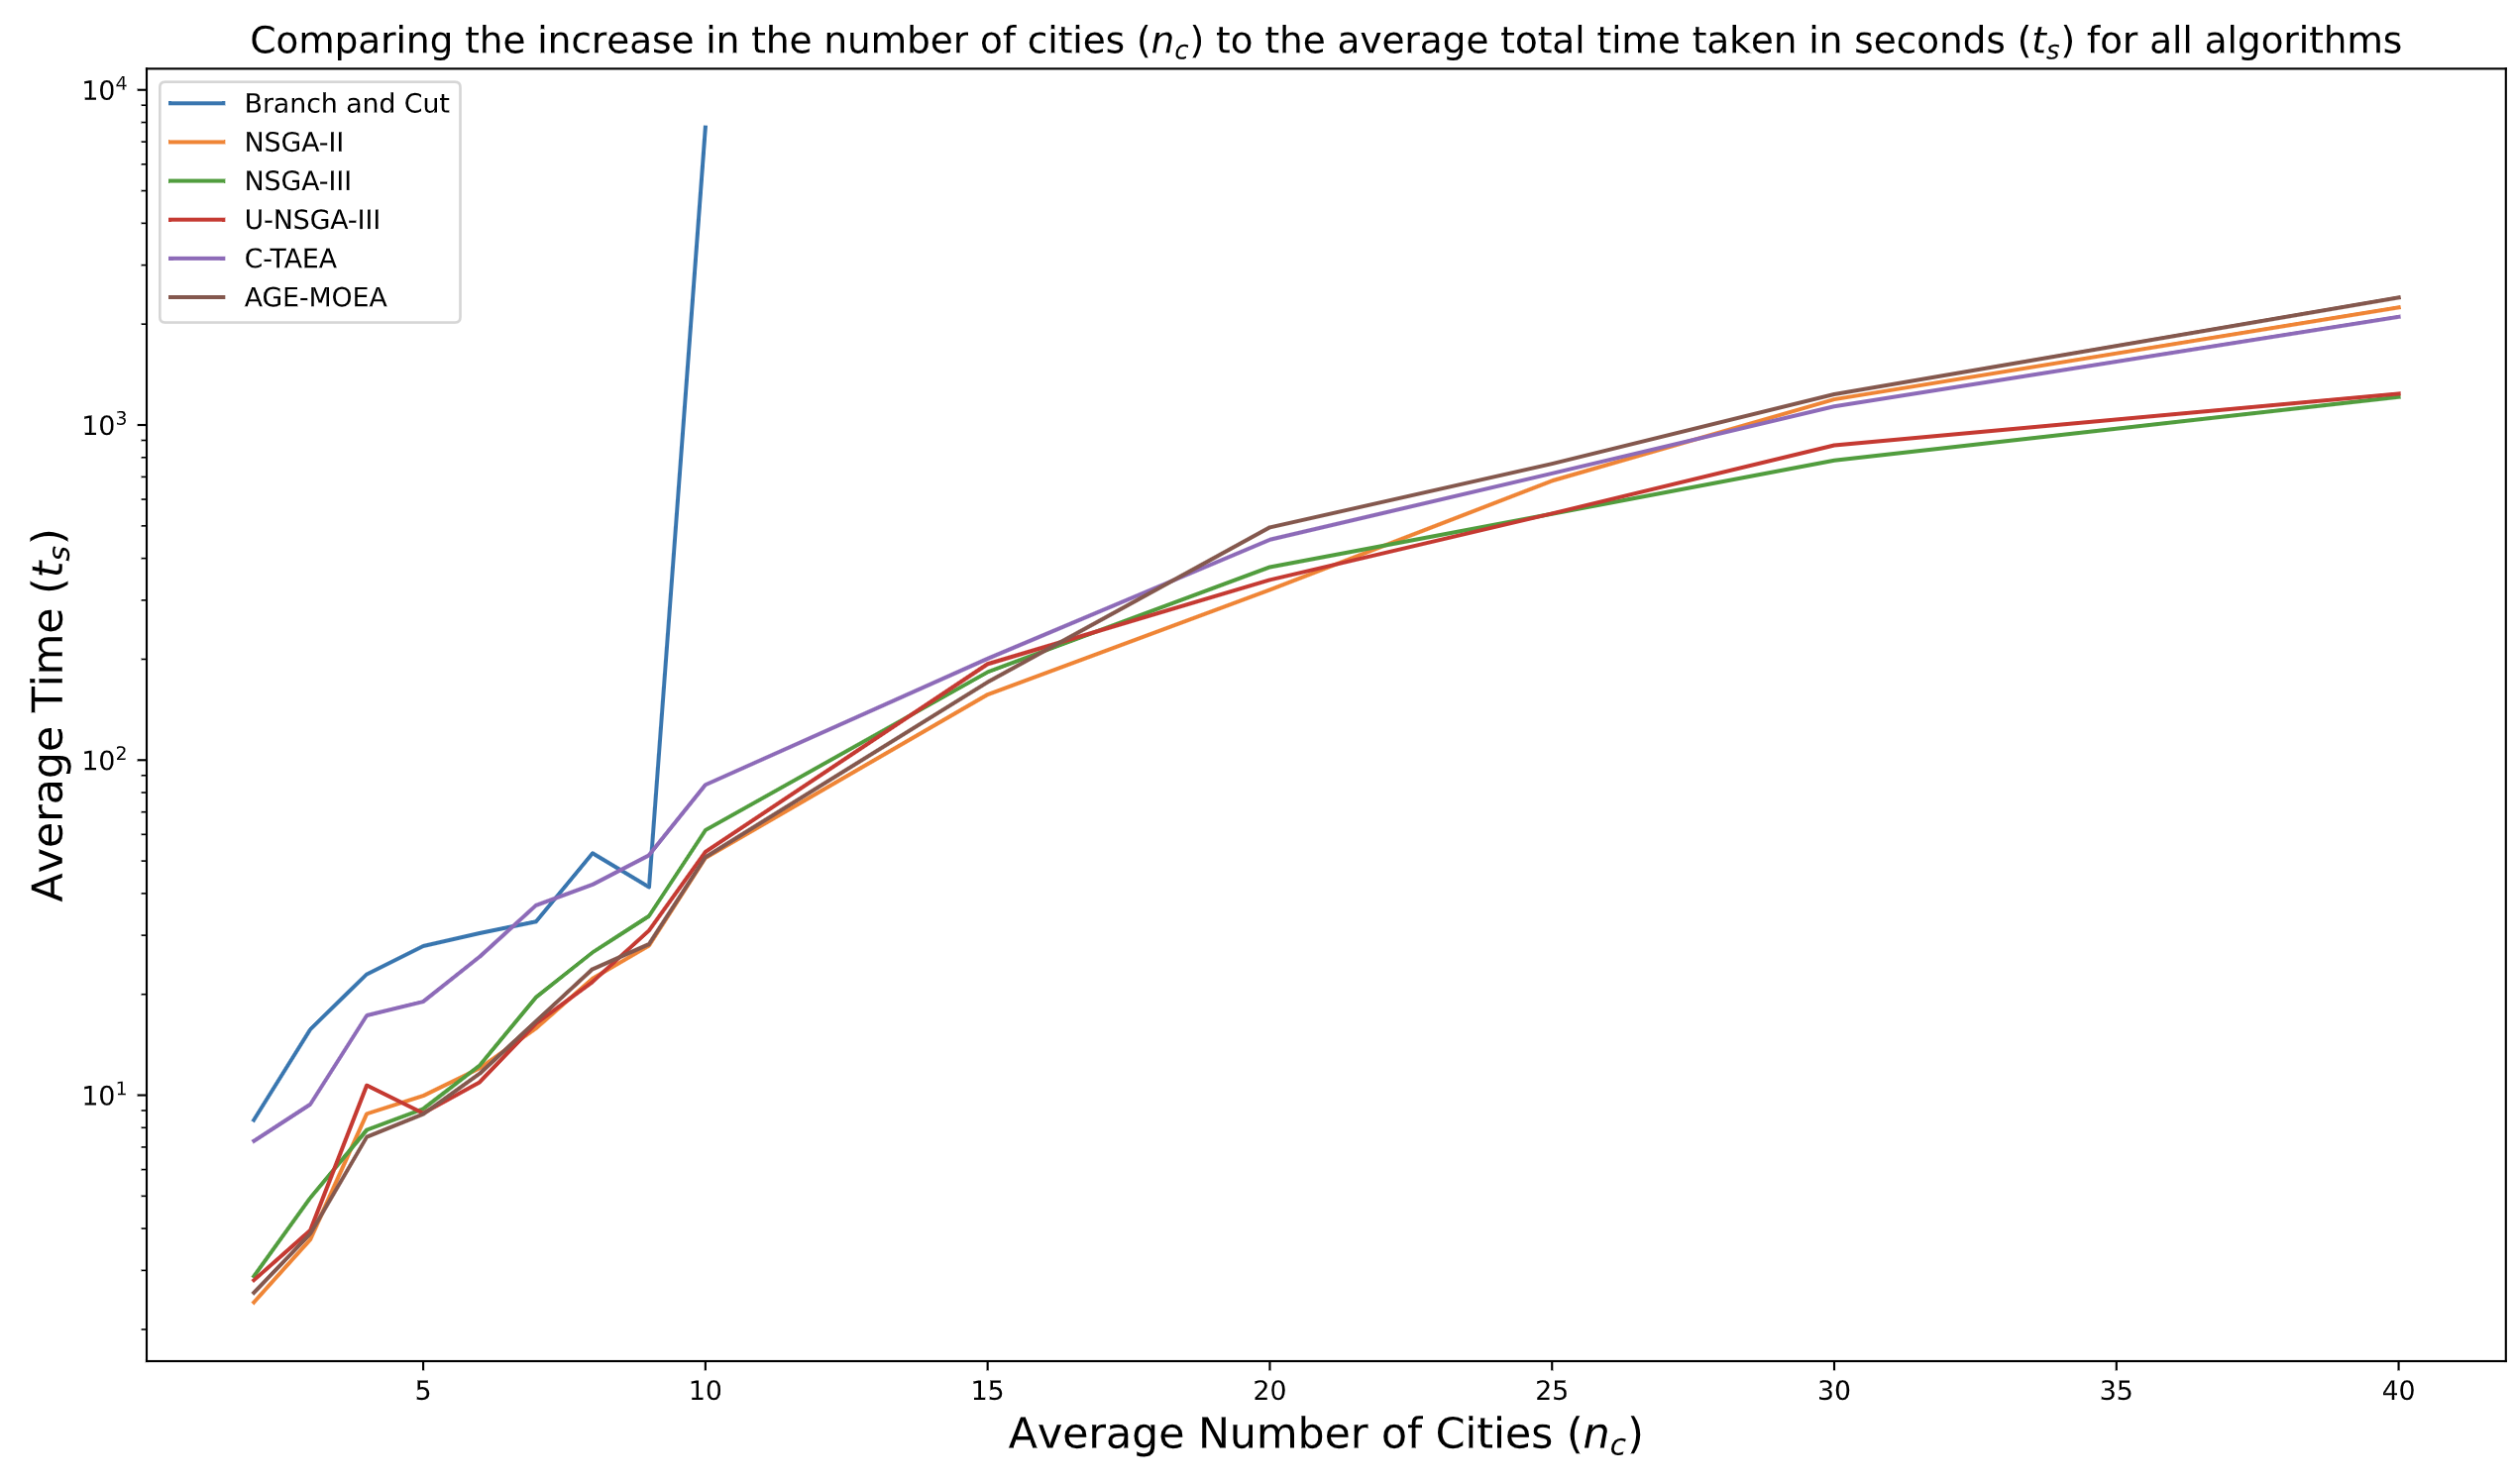
\includegraphics[width=\textwidth]{/results/log_scale_time_all.png}
    \caption{The average total time taken shown on a log scale for all algorithms.}
    \label{fig:log_time}
\end{figure}
\clearpage
\section{Hypervolume results}\label{sec:hv_res}
We took the average hypervolume for each city number, graph, and algorithm seed. Figure \ref{fig:hv_small} shows the result for the small-scale problems where we use all the algorithms, and figure \ref{fig:hv_large} shows the results for the large-scale algorithms. The MILP algorithm has the same average hypervolume as the evolutionary algorithms for problems with fewer cities. Additionally, as the problem size increases, the hypervolume of all the evolutionary algorithms is much higher. The hypervolume for NSGA-III is twice as high as the MILP solution for the nine city problems, and the other evolutionary algorithms behave similarly. For the large-scale problems, NSGA-II and AGE-MOEA reign supreme for 40, 30 and 25 cities. U-NSGA-III is the third best, finding the best results on average for 15 cities. C-TAEA provides the worst results for 15, 20, 25, and 30 cities. However catches up on 40 cities, with it being a bit better on average than NSGA-III.

\section{Number of solution results}\label{sec:num_sol_res}
As before, we obtain the average number of solutions for each city number, graph, and algorithm seed. Figure \ref{fig:sol_count_small} gives information on the average number of solutions for small-scale problems, and figure \ref{fig:sol_count_large} illustrates the average number for large-scale problems. Figure \ref{fig:sol_count_small} conveys that the NSGA-II and AGE-MOEA algorithms obtain the most solutions, with the highest number of solutions obtained by NSGA-II with six cities. NSGA-III and U-NSGA-III obtain the lowest amount of solutions on average. In addition, the CPLEX MILP always has the same number of seven solutions because we found one solution for each optimisation, including single-objective, bi-objective, and tri-objective problem formulations. Figure \ref{fig:sol_count_large} exhibits the same trend as in the small-scale problems, with fewer solutions as the problems get larger for all algorithms.
\begin{figure}[ht]
    \centering
    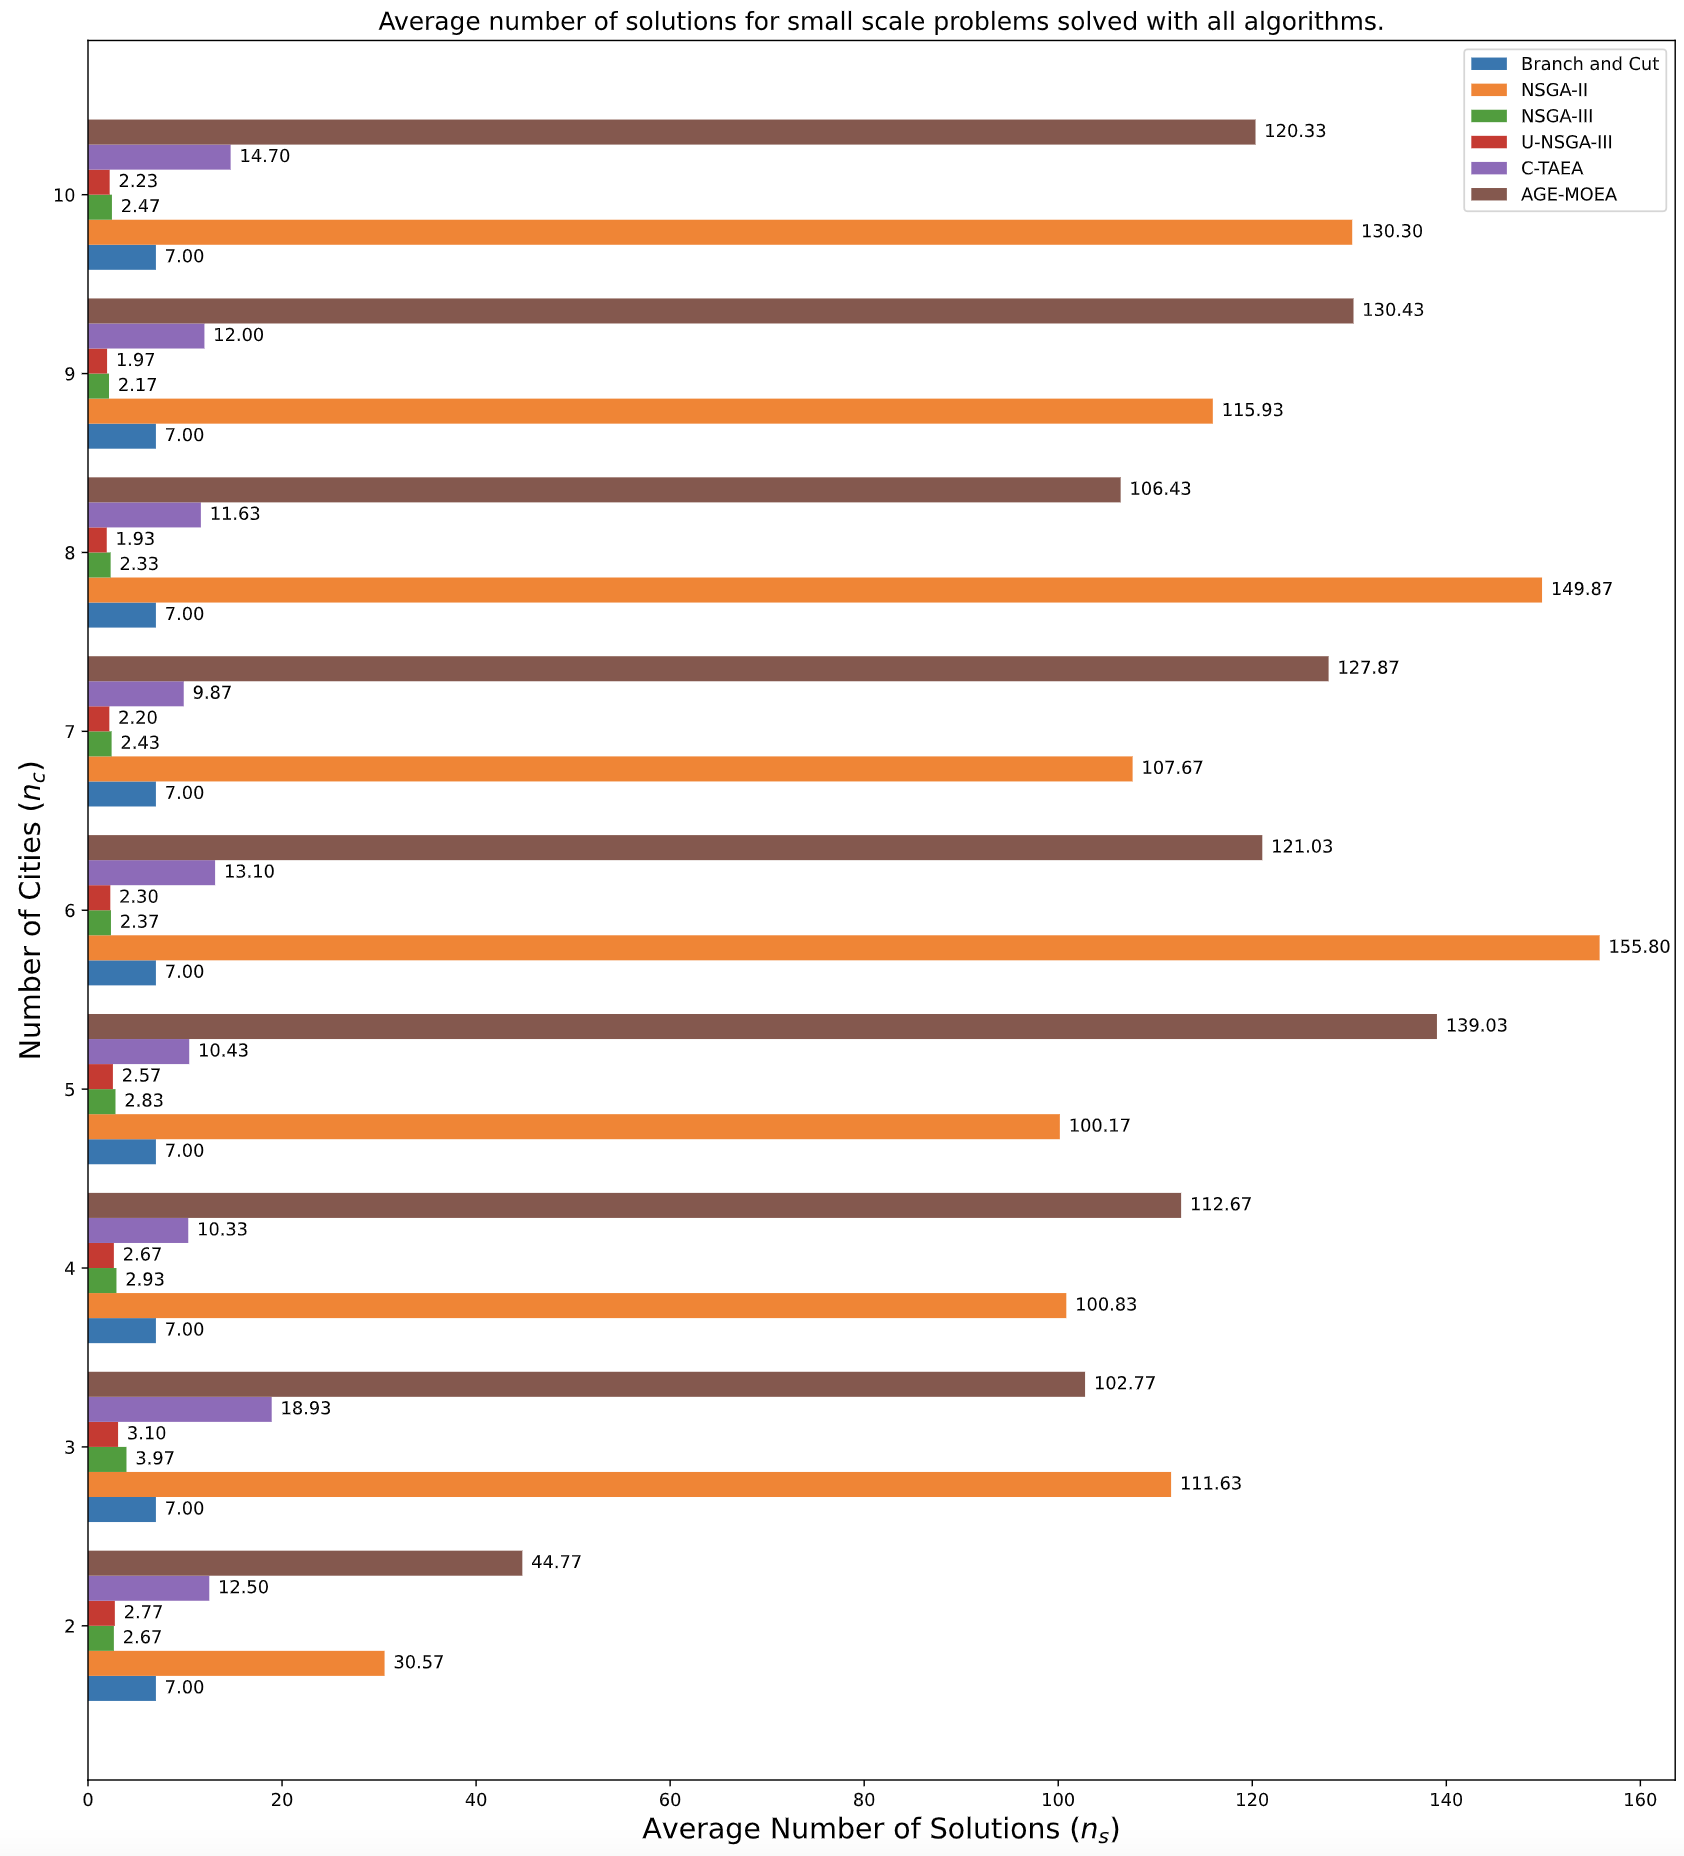
\includegraphics[width=\textwidth]{/results/solution_count_small_scale.png}
    \caption{The average number of solutions ($n_s$) for all number of cities ($n_c$) from two -- ten.}
    \label{fig:sol_count_small}
\end{figure}
\begin{figure}[ht]
    \centering
    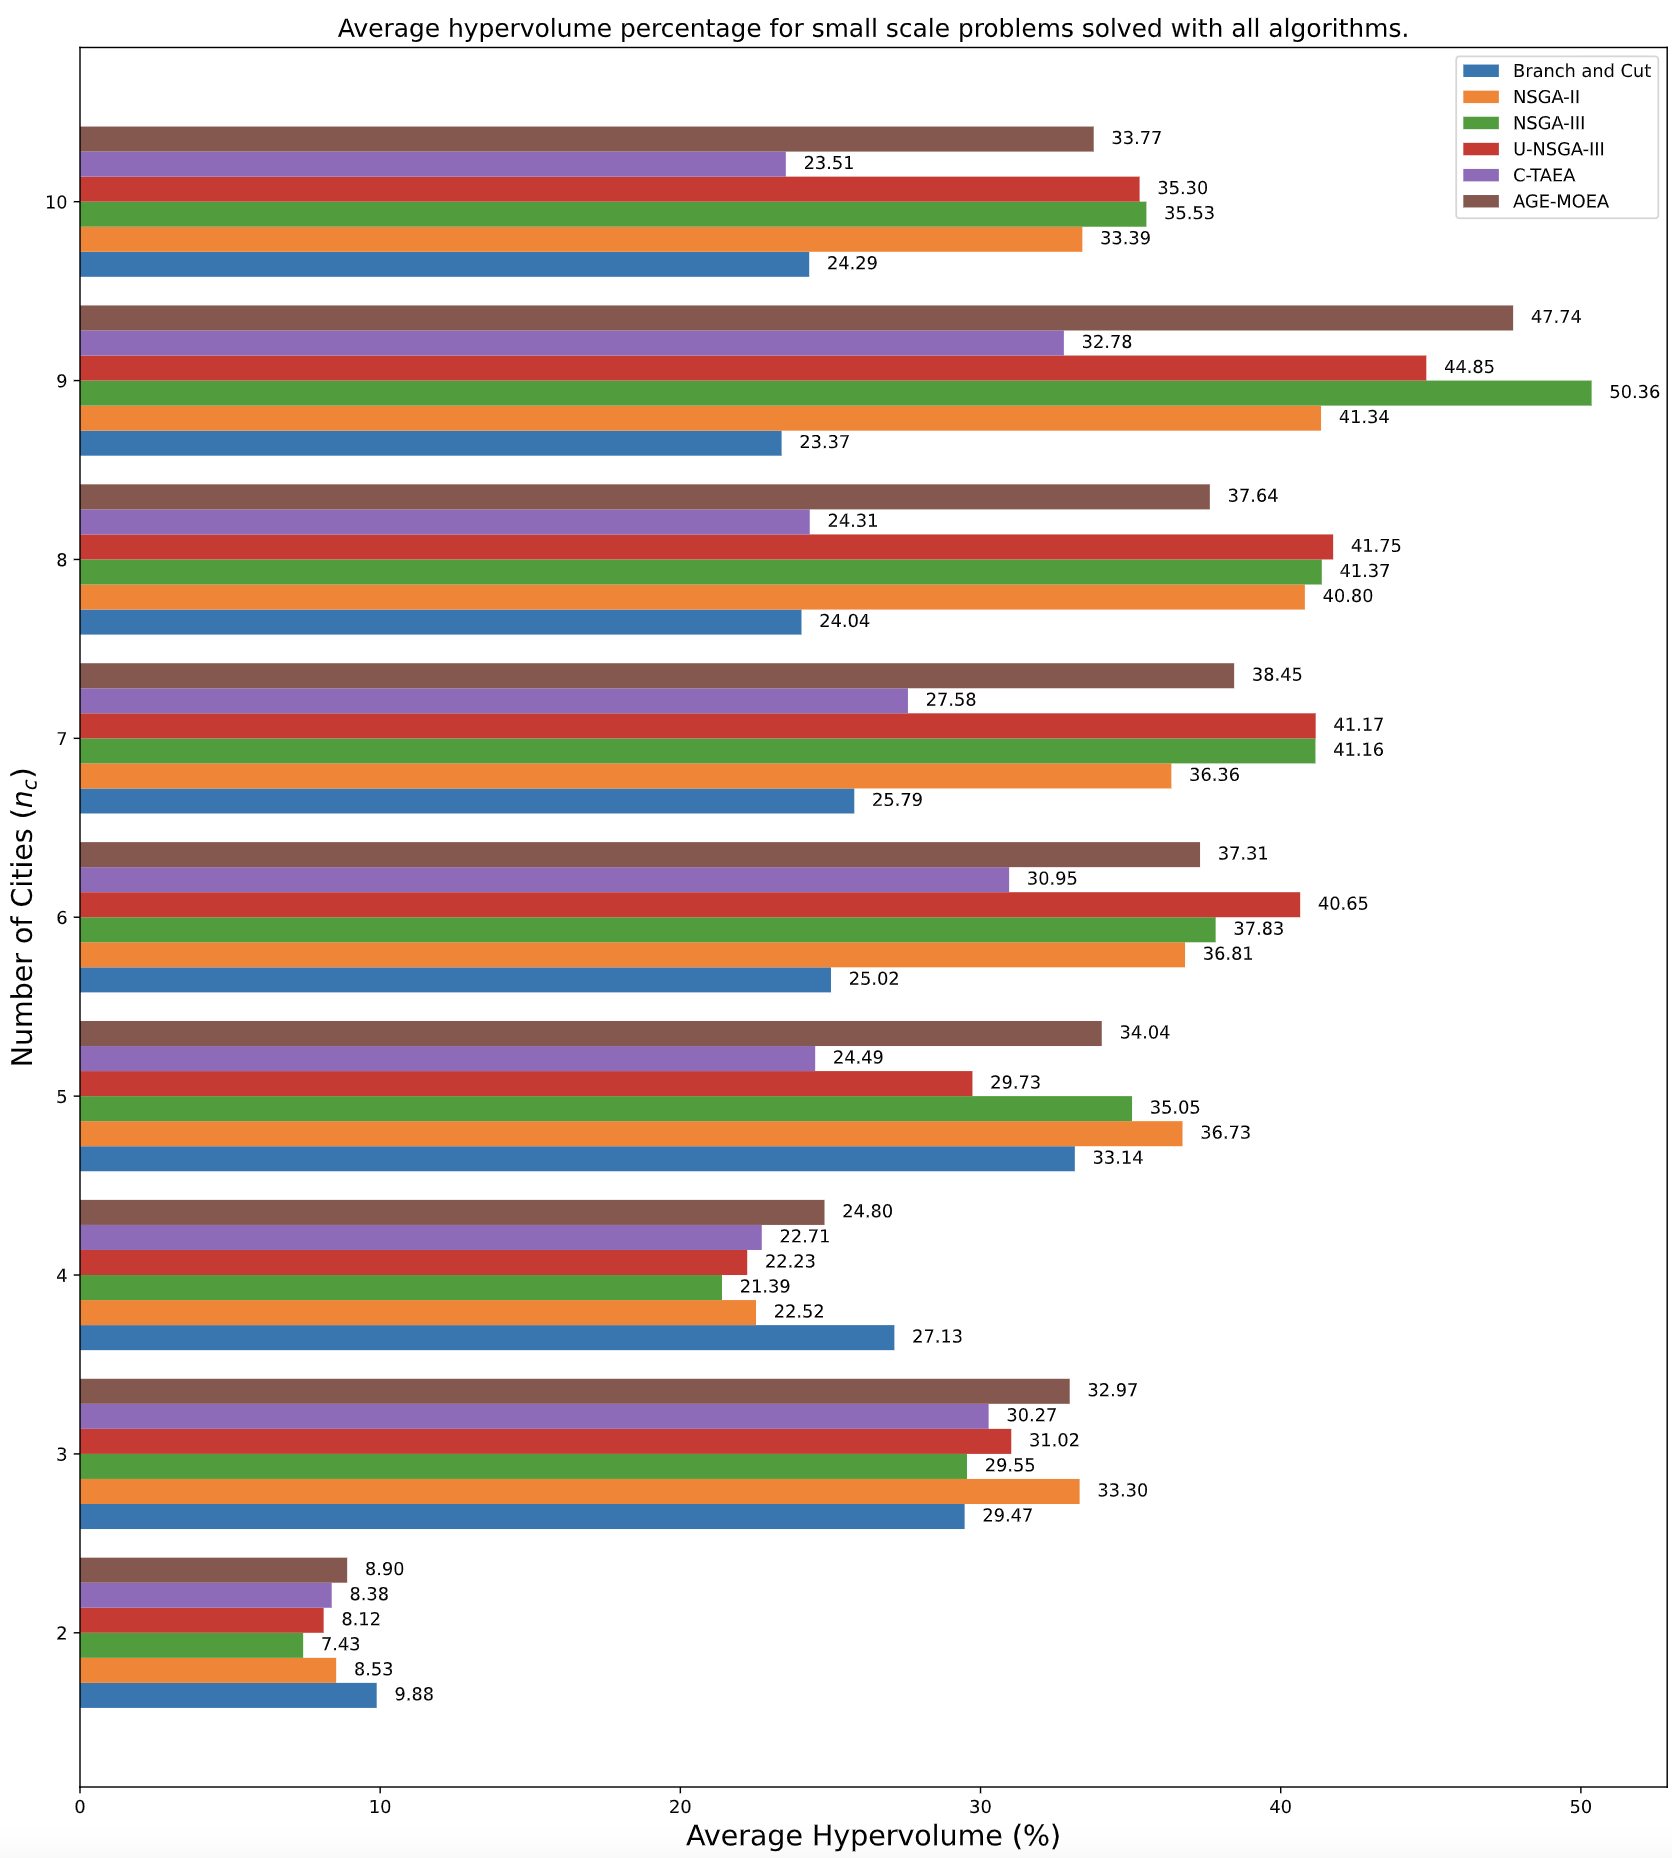
\includegraphics[width=\textwidth]{/results/hv_small_scale.png}
    \caption{The average hypervolume shown in percentages for small problems solved with all algorithms for cities 2 to 10.}
    \label{fig:hv_small}
\end{figure}
\begin{figure}[ht]
    \centering
    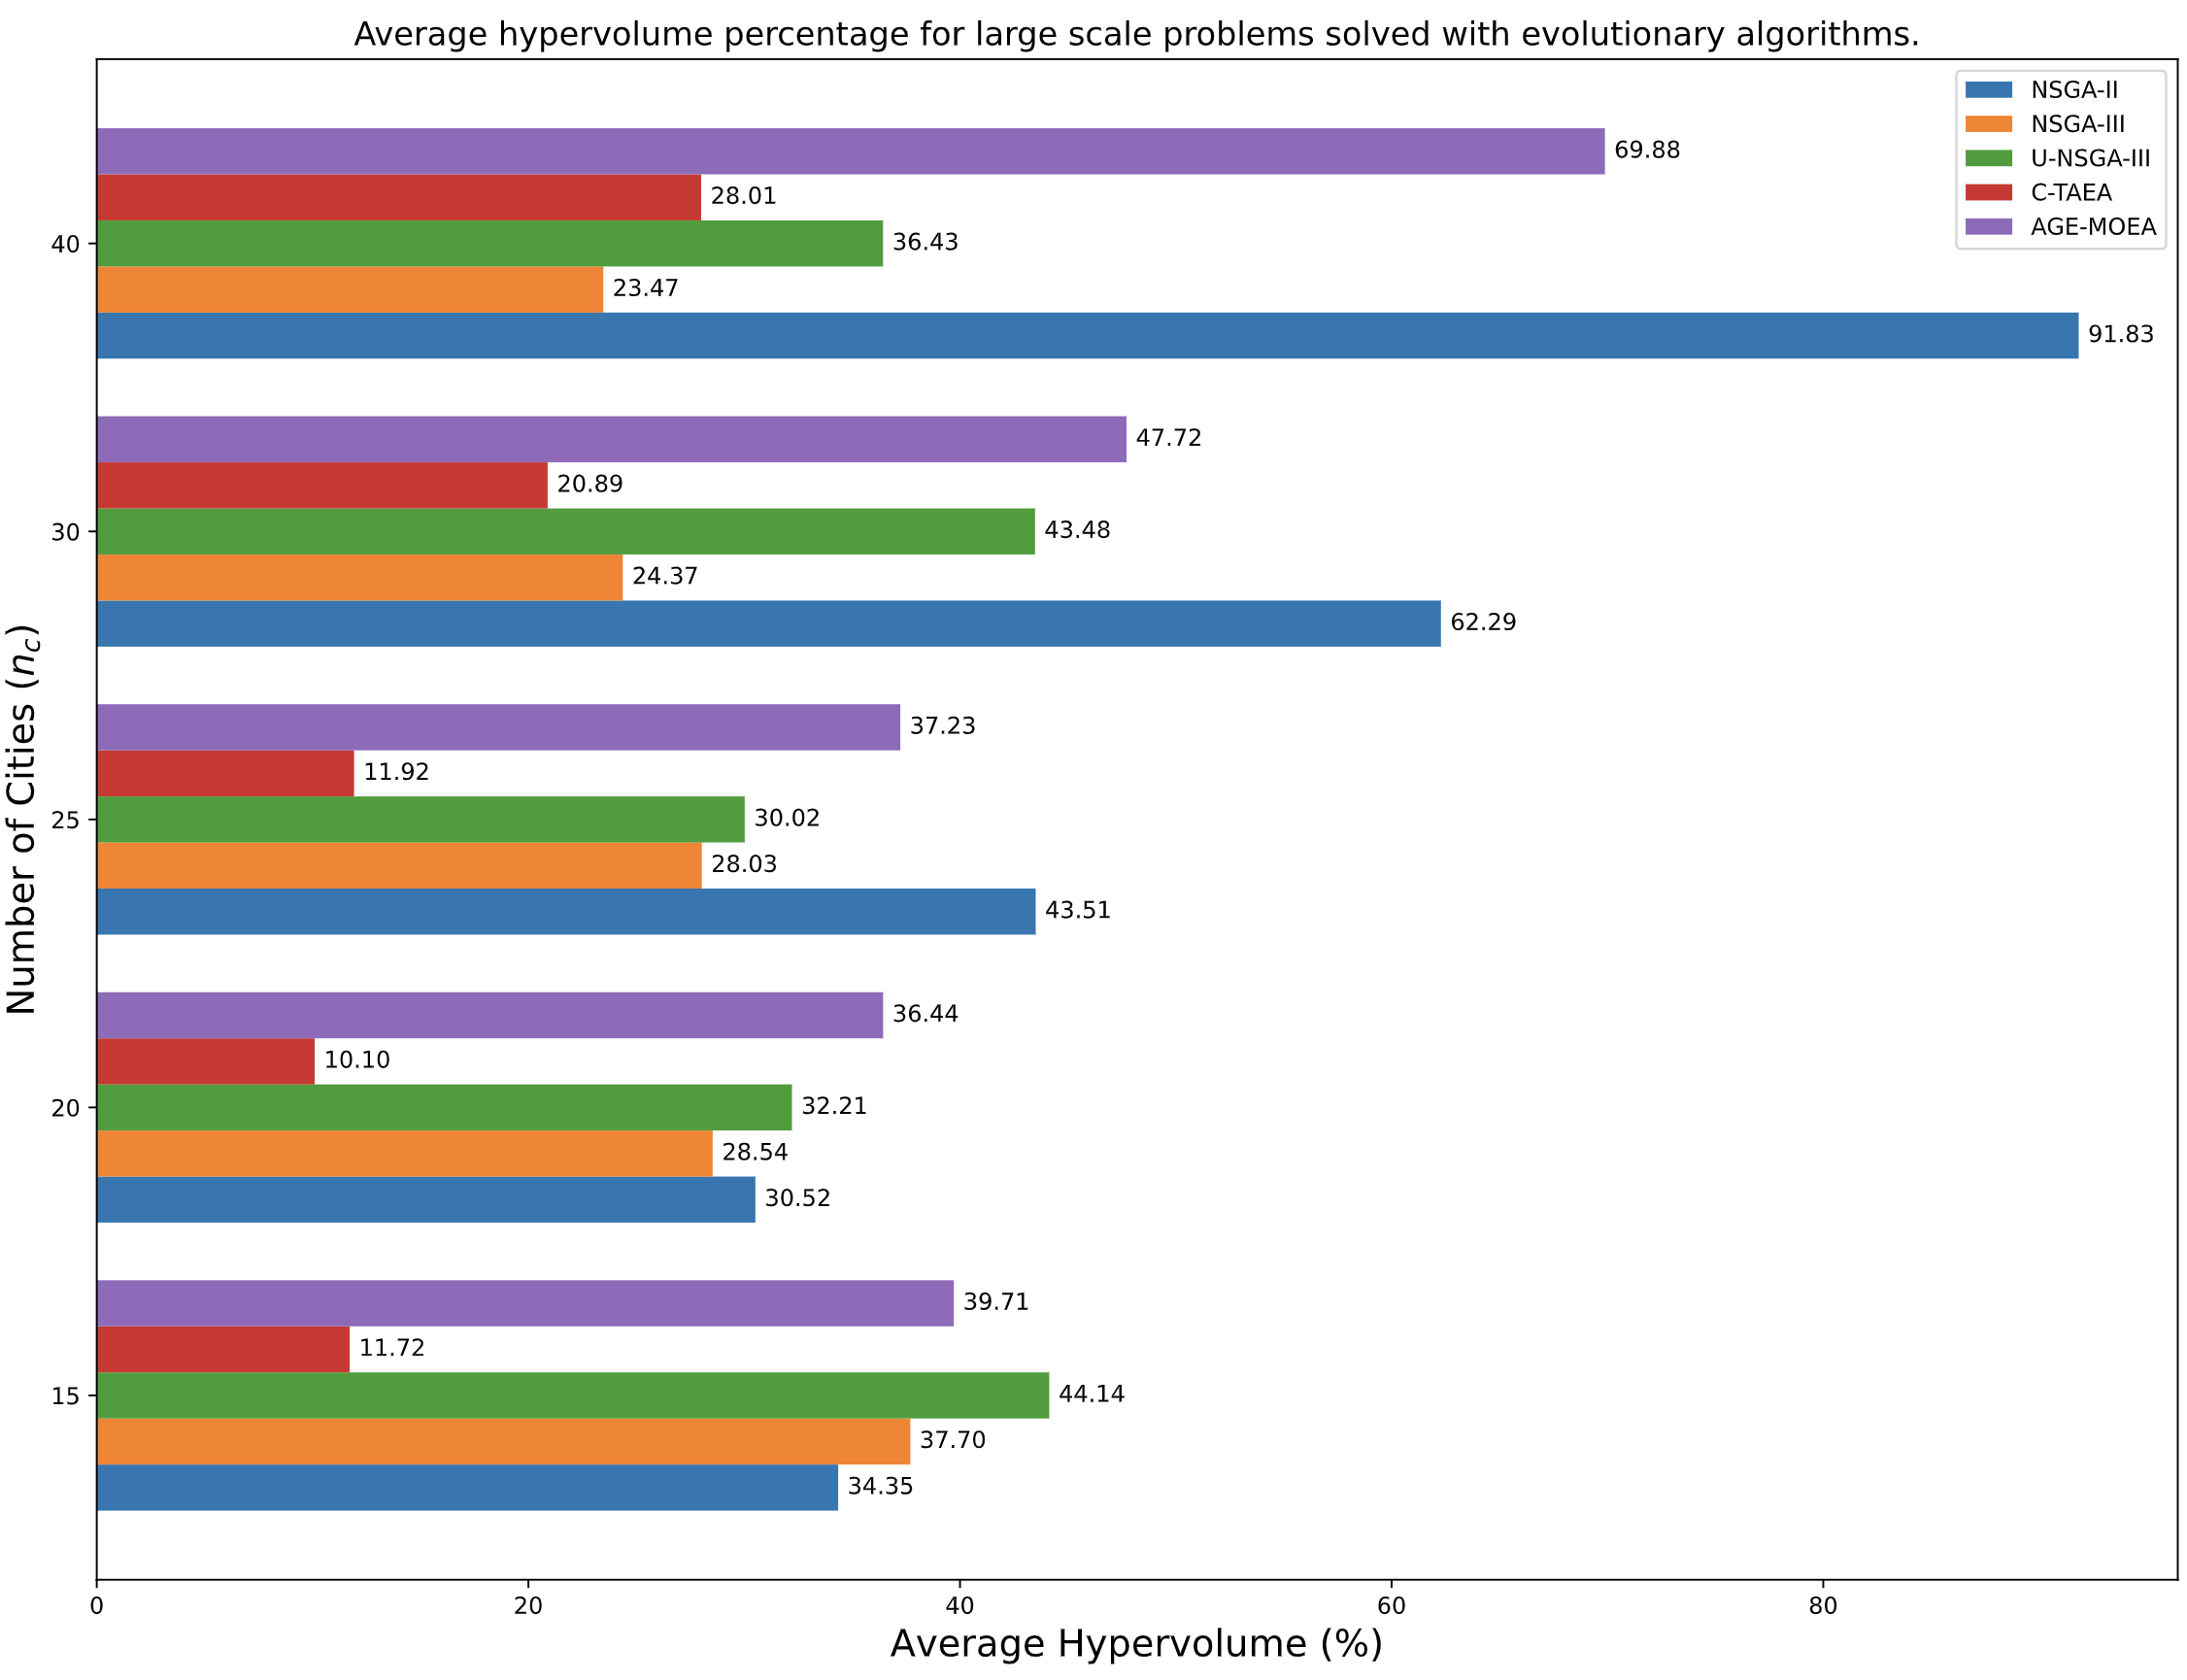
\includegraphics[width=\textwidth]{/results/hv_large_scale.png}
    \caption{The average hypervolume shown in percentages for large problems solved with evolutionary algorithms for cities $15$ -- $30$ and $40$.}
    \label{fig:hv_large}
\end{figure}
\begin{figure}[ht]
    \centering
    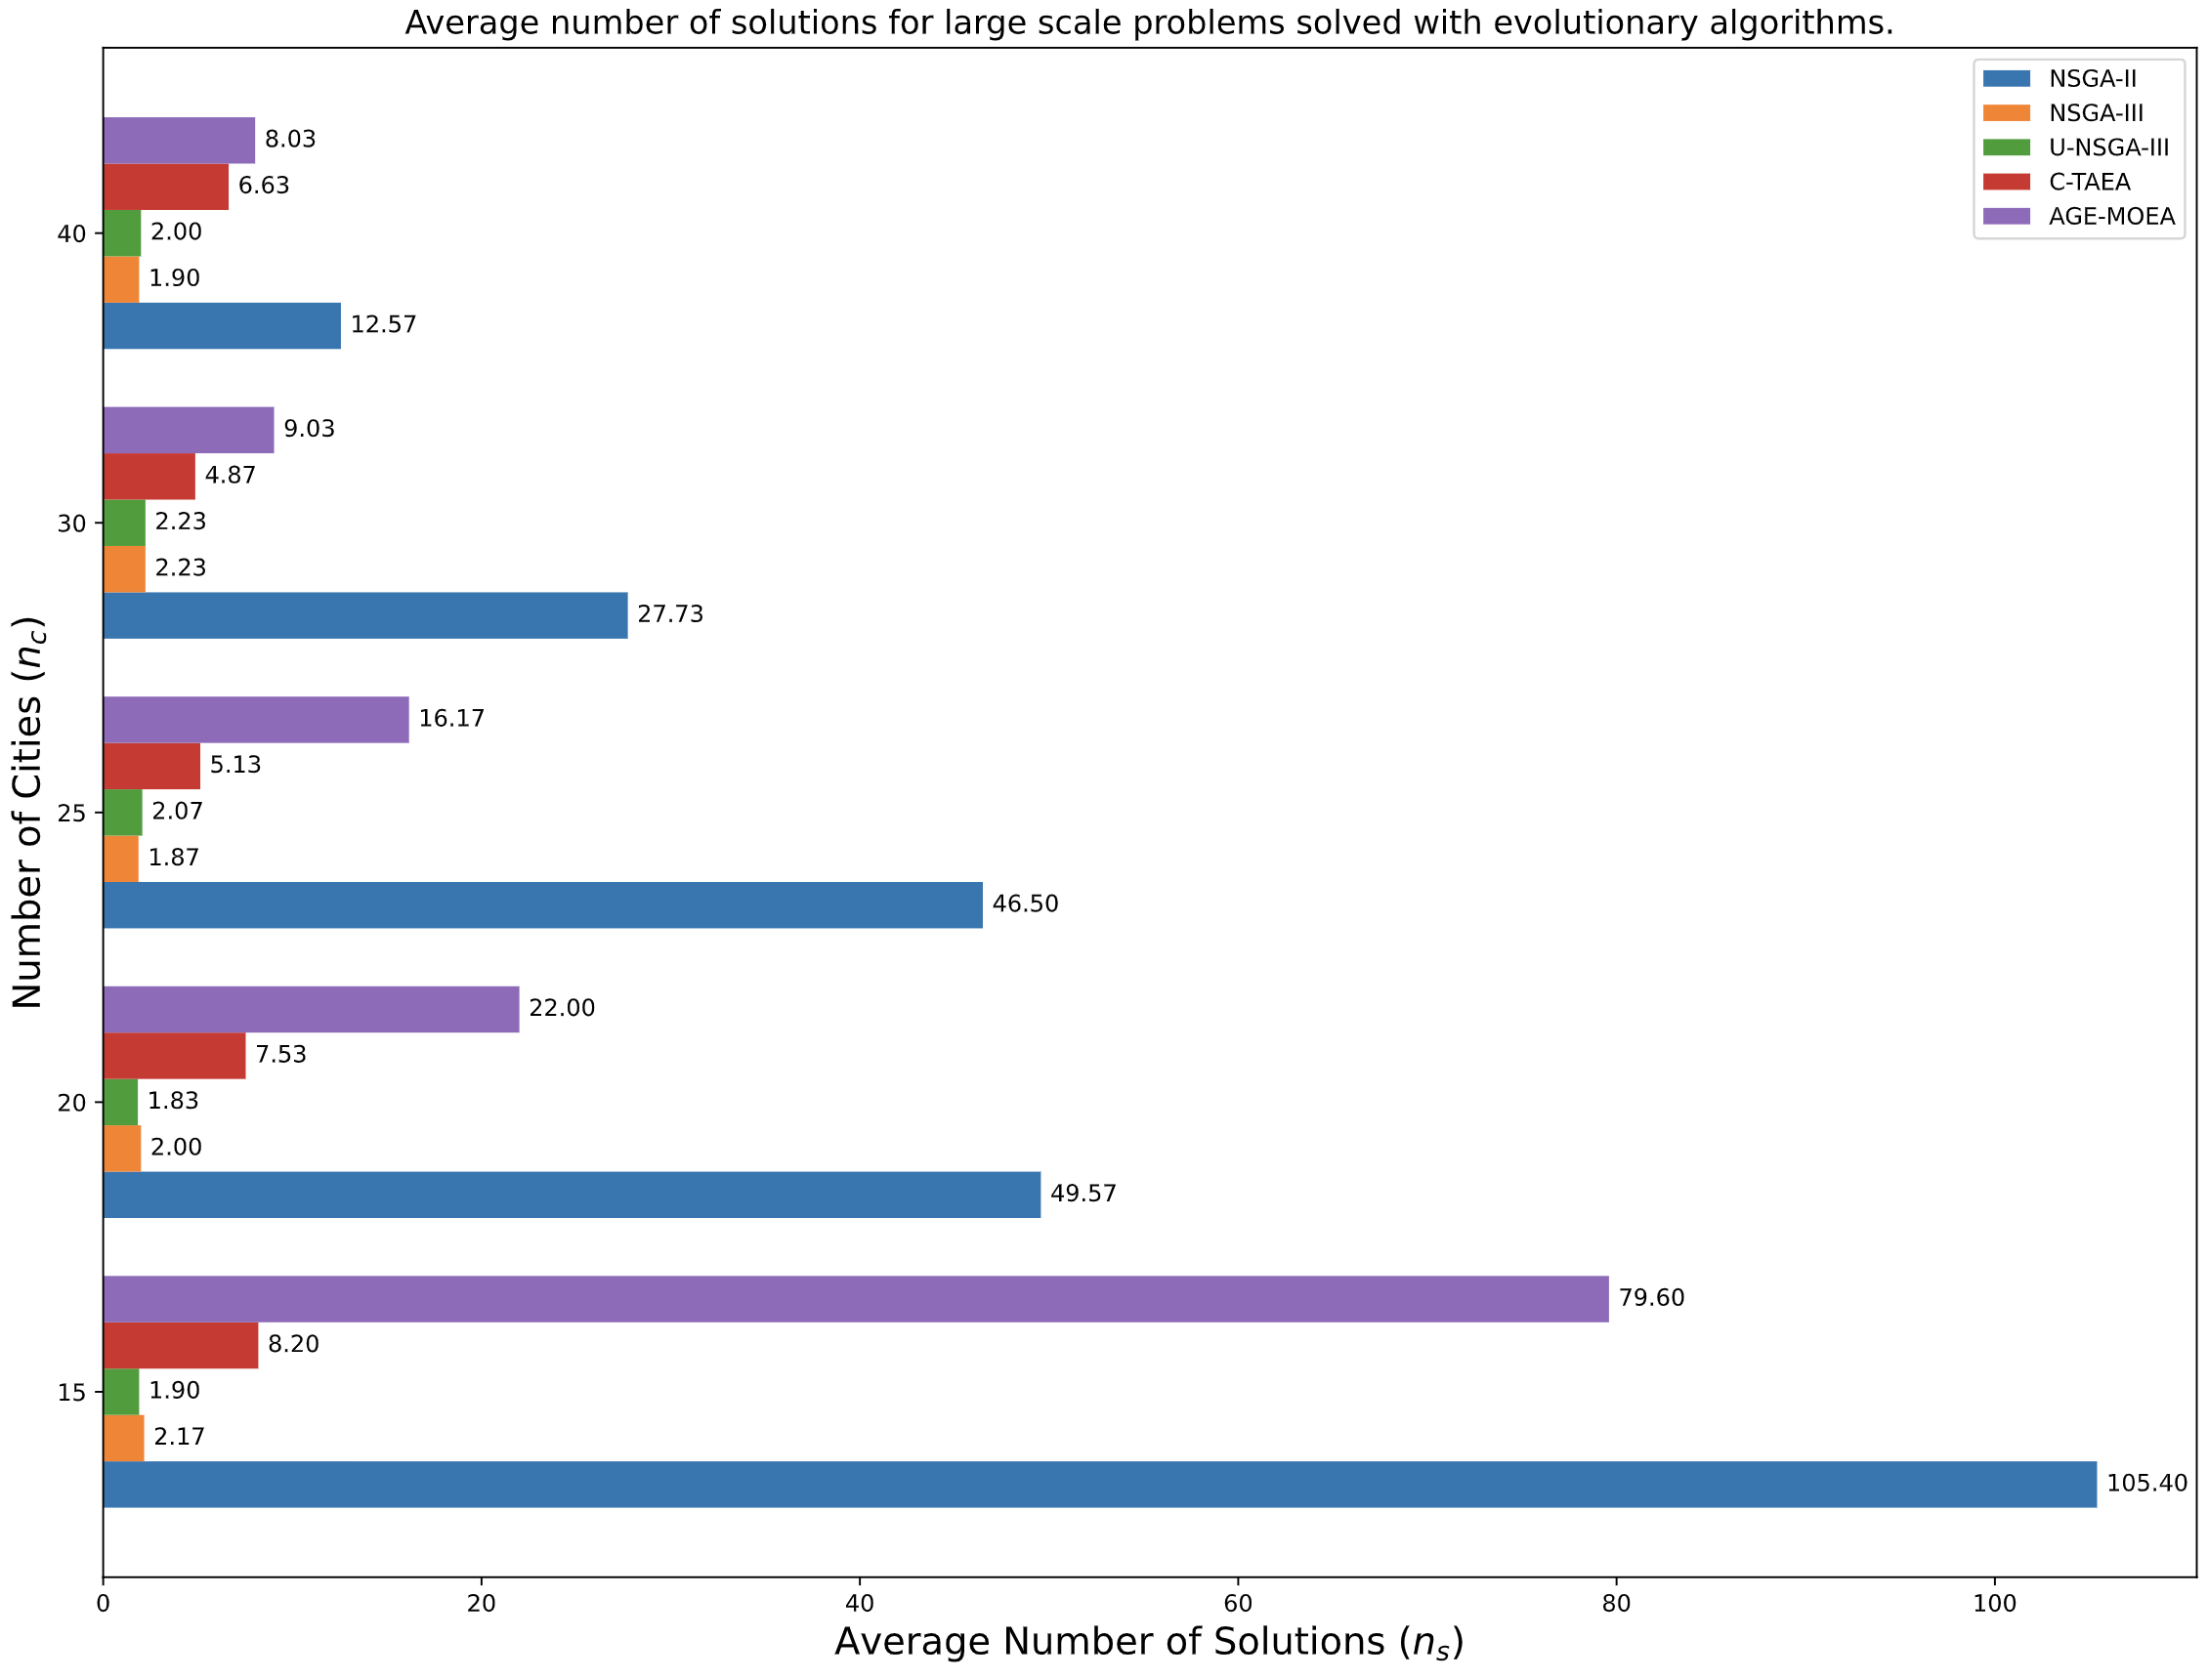
\includegraphics[width=\textwidth]{/results/solution_count_large_scale.png}
    \caption{The average number of solutions ($n_s$) for all number of cities ($n_c$) from 15 -- 30 and 40.}
    \label{fig:sol_count_large}
\end{figure}
\clearpage
\section{Solution results}\label{sec:sol_res}
Figures \ref{fig:boxplot_2_to_5} -- \ref{fig:boxplot_15_to_40} convey the distribution of the total cost, land usage, and health impact obtained for each average city count, graph, and algorithm seed. Figure \ref{fig:boxplot_2_to_5} shows this distribution for small-scale problems, from two to five average cities. Figure \ref{fig:boxplot_6_to_10} illustrates the distributions for medium-sized graphs of six to ten cities. Finally, figure \ref{fig:boxplot_15_to_30} displays the distributions for large-scale graphs of sizes $15$ to $30$ average cities, which use all evolutionary algorithms. For $40$ cities, we display two versions in figure \ref{fig:boxplot_40}: the original version that uses all the evolutionary algorithms solutions and a modified version that removes the C-TAEA algorithm.
\\\\
For all the boxplots, the straight line shows the median value of the objective solutions, and the dotted line displays the mean value. Furthermore, three axes exist for each city plot, one the total cost ($f_c$) given in Swiss francs (CHF). The average land use stress ($f_u$), calculated by using equation \ref{ratio}, and the total public health impact ($f_h$) that uses DALYs.
\\\\
In figure \ref{fig:2_cities}, we do not see many variations in the solutions obtained for all algorithms. Furthermore, the means of the cost objective are very similar, and the medians are on the same level. The CPLEX branch and cut has the lowest interquartile range (IQR) for this objective, the highest minimum value, and the lowest maximum value. For the land use objective, the spread of the solutions is very similar, and the interquartile ranges do not differ much. All solutions found the same minimum value in the public health impact objective. However, the branch and cut algorithm again finds the lowest maximum value. For all objectives, we do not see any outliers.
\\\\
In figure \ref{fig:3_cities}, we already see a vast difference compared with \ref{fig:2_cities}. The first very striking event is that the branch and cut algorithm on the cost and land use objective shows a meagre IQR, which means that the spread of the solutions is also shallow. In addition, the C-TAEA algorithm also has a low IQR for the land usage objective. U-NSGA-III finds the highest valued outliers and also the highest amount of upper quartile outliers. For the public health impact, all algorithms show a minimal IQR. The branch and cut algorithm has the lowest mean for all solutions for the total cost and the highest for land use and health impact.
Figure \ref{fig:5_cities} is very similar to figure \ref{fig:3_cities}, with a very limited IQR for the cost and land use objectives. 
\\\\
For figures \ref{fig:4_cities}, the branch and cut algorithm obtains an extensive IQR for the cost objective, which is very similar to the U-NSGA-III algorithm. However, with the benefit of finding lower-cost solutions compared to U-NSGA-III. In the land use objective, the branch and cut has a limited range with no upper $25\%$ and lower $25\%$ of values existing. On the other hand, the evolutionary algorithms are very similar in achieving high interquartile ranges.
\\\\
When looking into the medium-sized solutions in figure \ref{fig:boxplot_6_to_10}, we see that the interquartile ranges start to differ a lot with the C-TAEA algorithm achieving an immense IQR for the land use objective in figures \ref{fig:6_cities}, \ref{fig:7_cities}, and \ref{fig:9_cities}. The evolutionary algorithms obtain a very high spread of solutions. However, they also obtain many more outliers than the branch and cut algorithm. For example, in figure \ref{fig:9_cities}, in the land use objective, the AGE-MOEA, U-NSGA-III and NSGA-III algorithms find many outliers with AGE-MOEA finding a total of six outliers with a low spread of solutions. For figure \ref{fig:10_cities}, all evolutionary algorithms find a higher spread of solutions or a lower value than the branch and cut algorithm.
\\\\
For large problems, the spread of solutions becomes much less, with the highest IQR found in figure \ref{fig:15_cities} by the C-TAEA algorithm. NSGA-II also finds a high solution spread for the average land usage objective. For figure \ref{fig:20_cities}, a much lower IQR for all evolutionary algorithms exists, with NSGA-II finding the lowest average cost across all the different evolutionary algorithms. In addition, NSGA-III finds three very high outliers across all three objectives. In figure \ref{fig:25_cities}, the spread of the solutions starts to increase again, with the IQR being very similar across all three objectives for all algorithms. Interestingly, there are many trade-offs across all of the evolutionary algorithms, with many being better in two objectives but one objective being worse than all the other algorithms.
Figure \ref{fig:30_cities} displays a small spread of solutions, as also seen in figure \ref{fig:20_cities}. NSGA-II shows the smallest spread, finding the minimum solutions over all the objectives and having the lowest average solution value for three objectives. Furthermore, NSGA-II does not have many high outliers, with the highest amount of outliers found by U-NSGA-III and C-TAEA, respectively.
\\\\
For the 40 city problem, in figure \ref{fig:40_cities}, the NSGA-III, C-TAEA, and U-NSGA-III algorithms, to stay in the feasible region, start to select a lot of landfill facilities, which induces a very high land usage. NSGA-II still finds the minimum across all three objectives. Furthermore, the IQR of the solutions found by NSGA-II are all low enough to be minimal solutions for the other algorithms. U-NSGA-III, NSGA-III, and C-TAEA have the highest spread of solutions according to figure \ref{fig:40_cities}.

% \begin{figure}
%     \centering
%     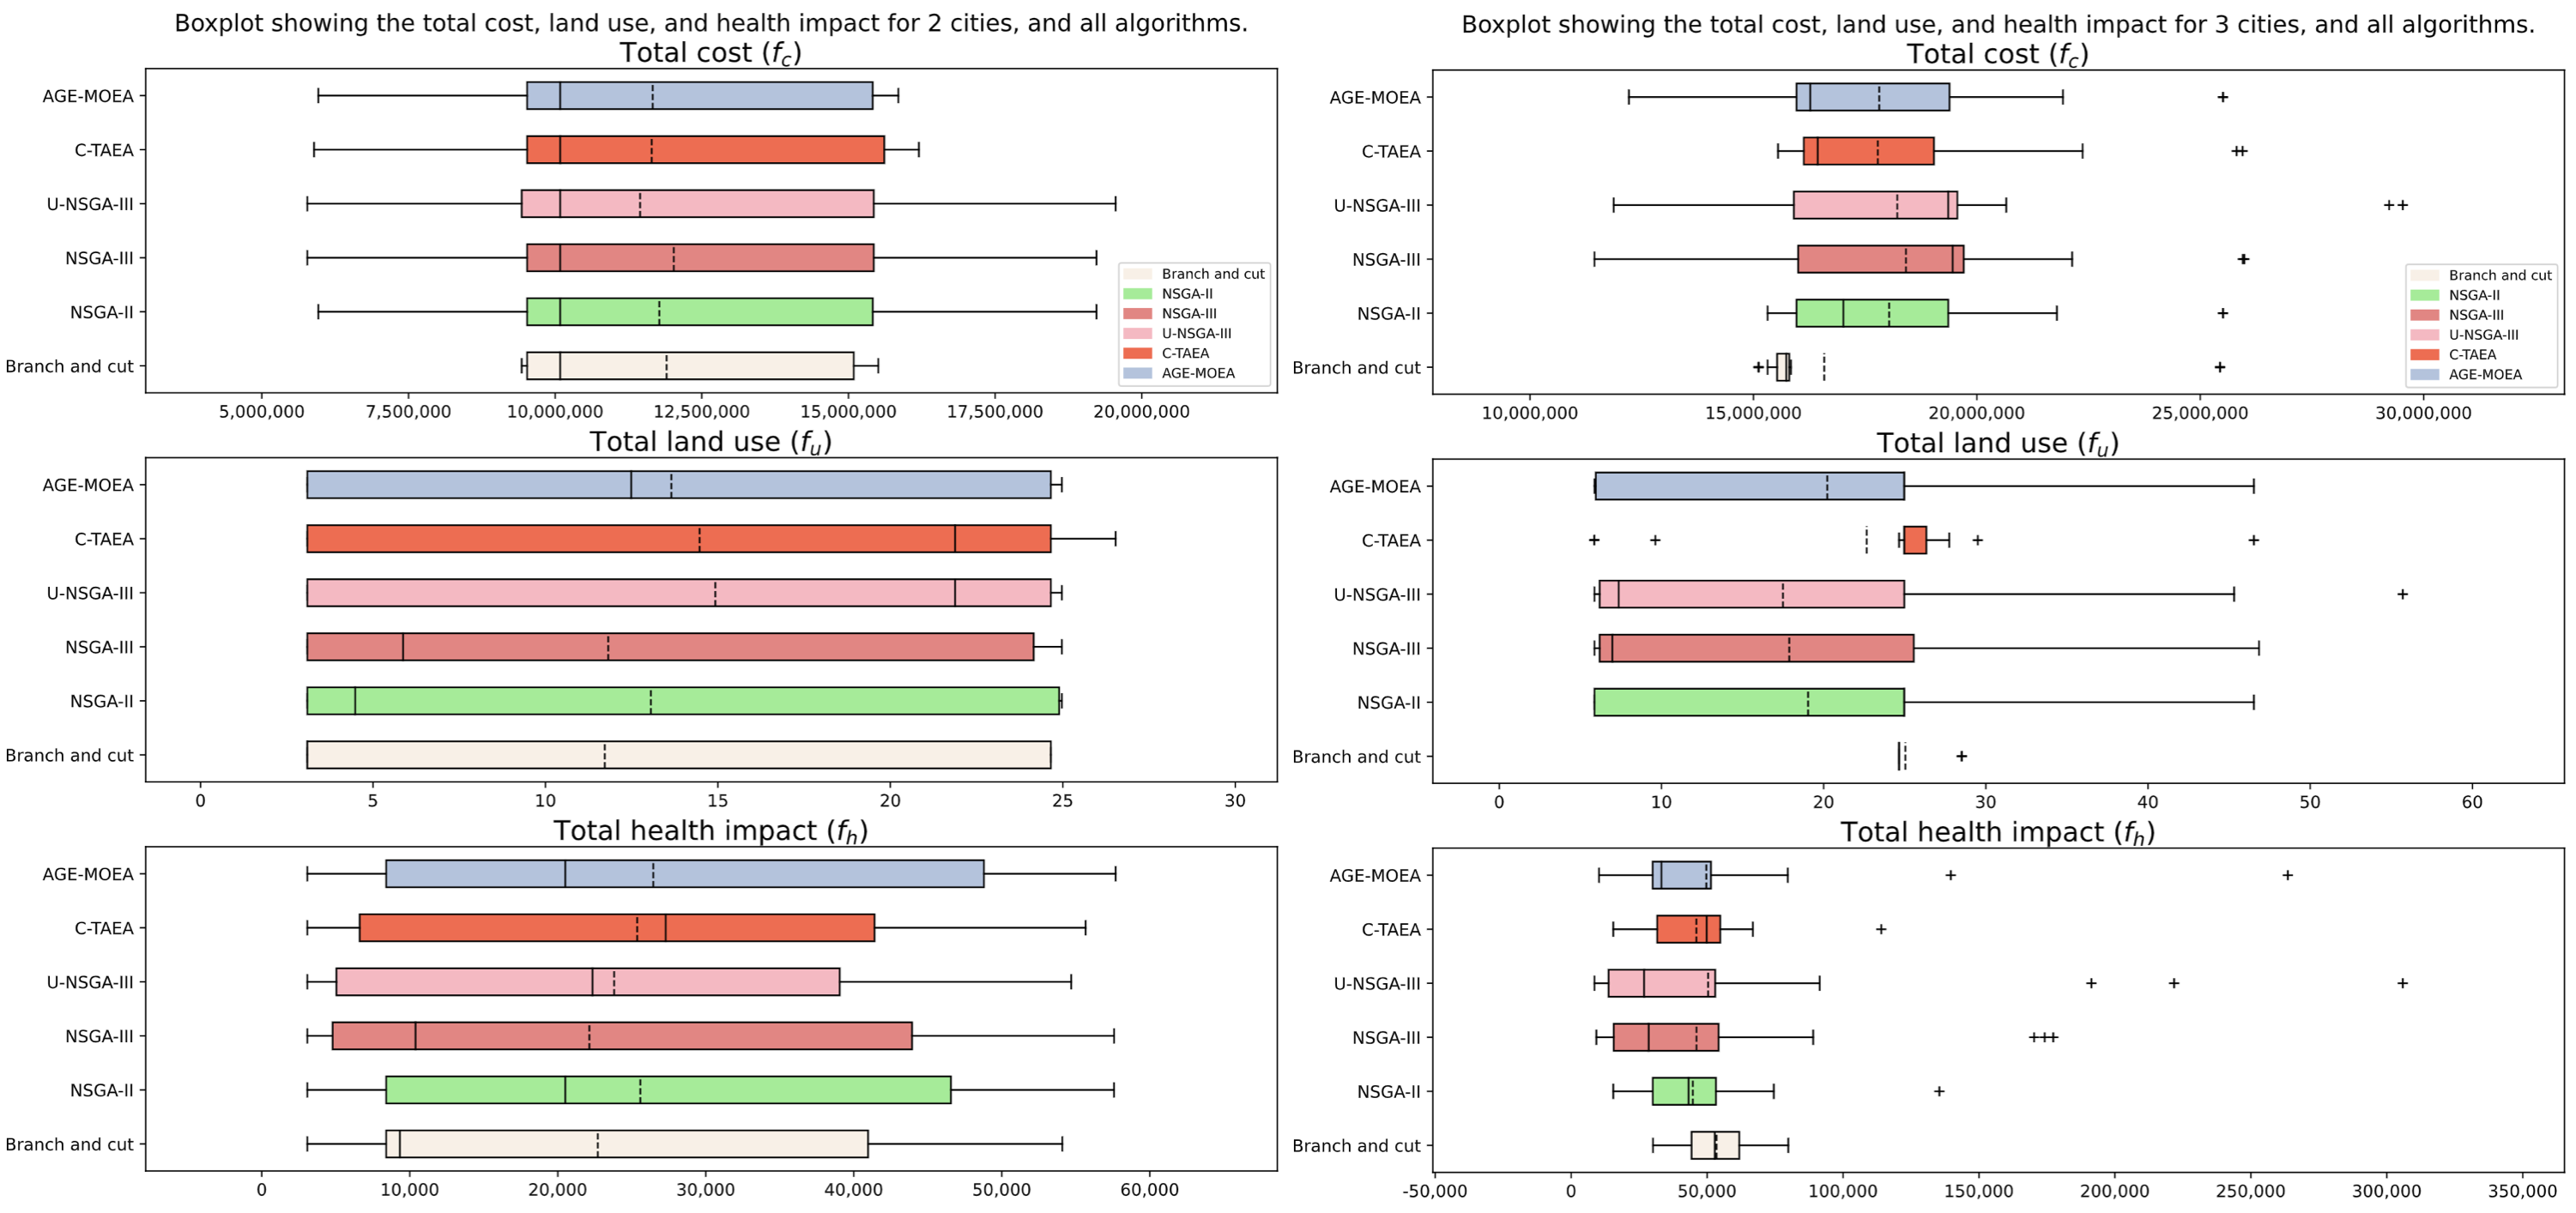
\includegraphics[width=\linewidth]{/results/box_23.png}
%     \caption{Boxplots showing the total cost, land usage and health impact for all algorithms. \textit{Left}, image for two cities; \textit{right}, image for three cities.}
%     \label{fig:my_label}
% \end{figure}

\begin{figure}[ht]
\centering
\noindent\makebox[\textwidth]{
\begin{subfigure}{0.4\paperwidth}

    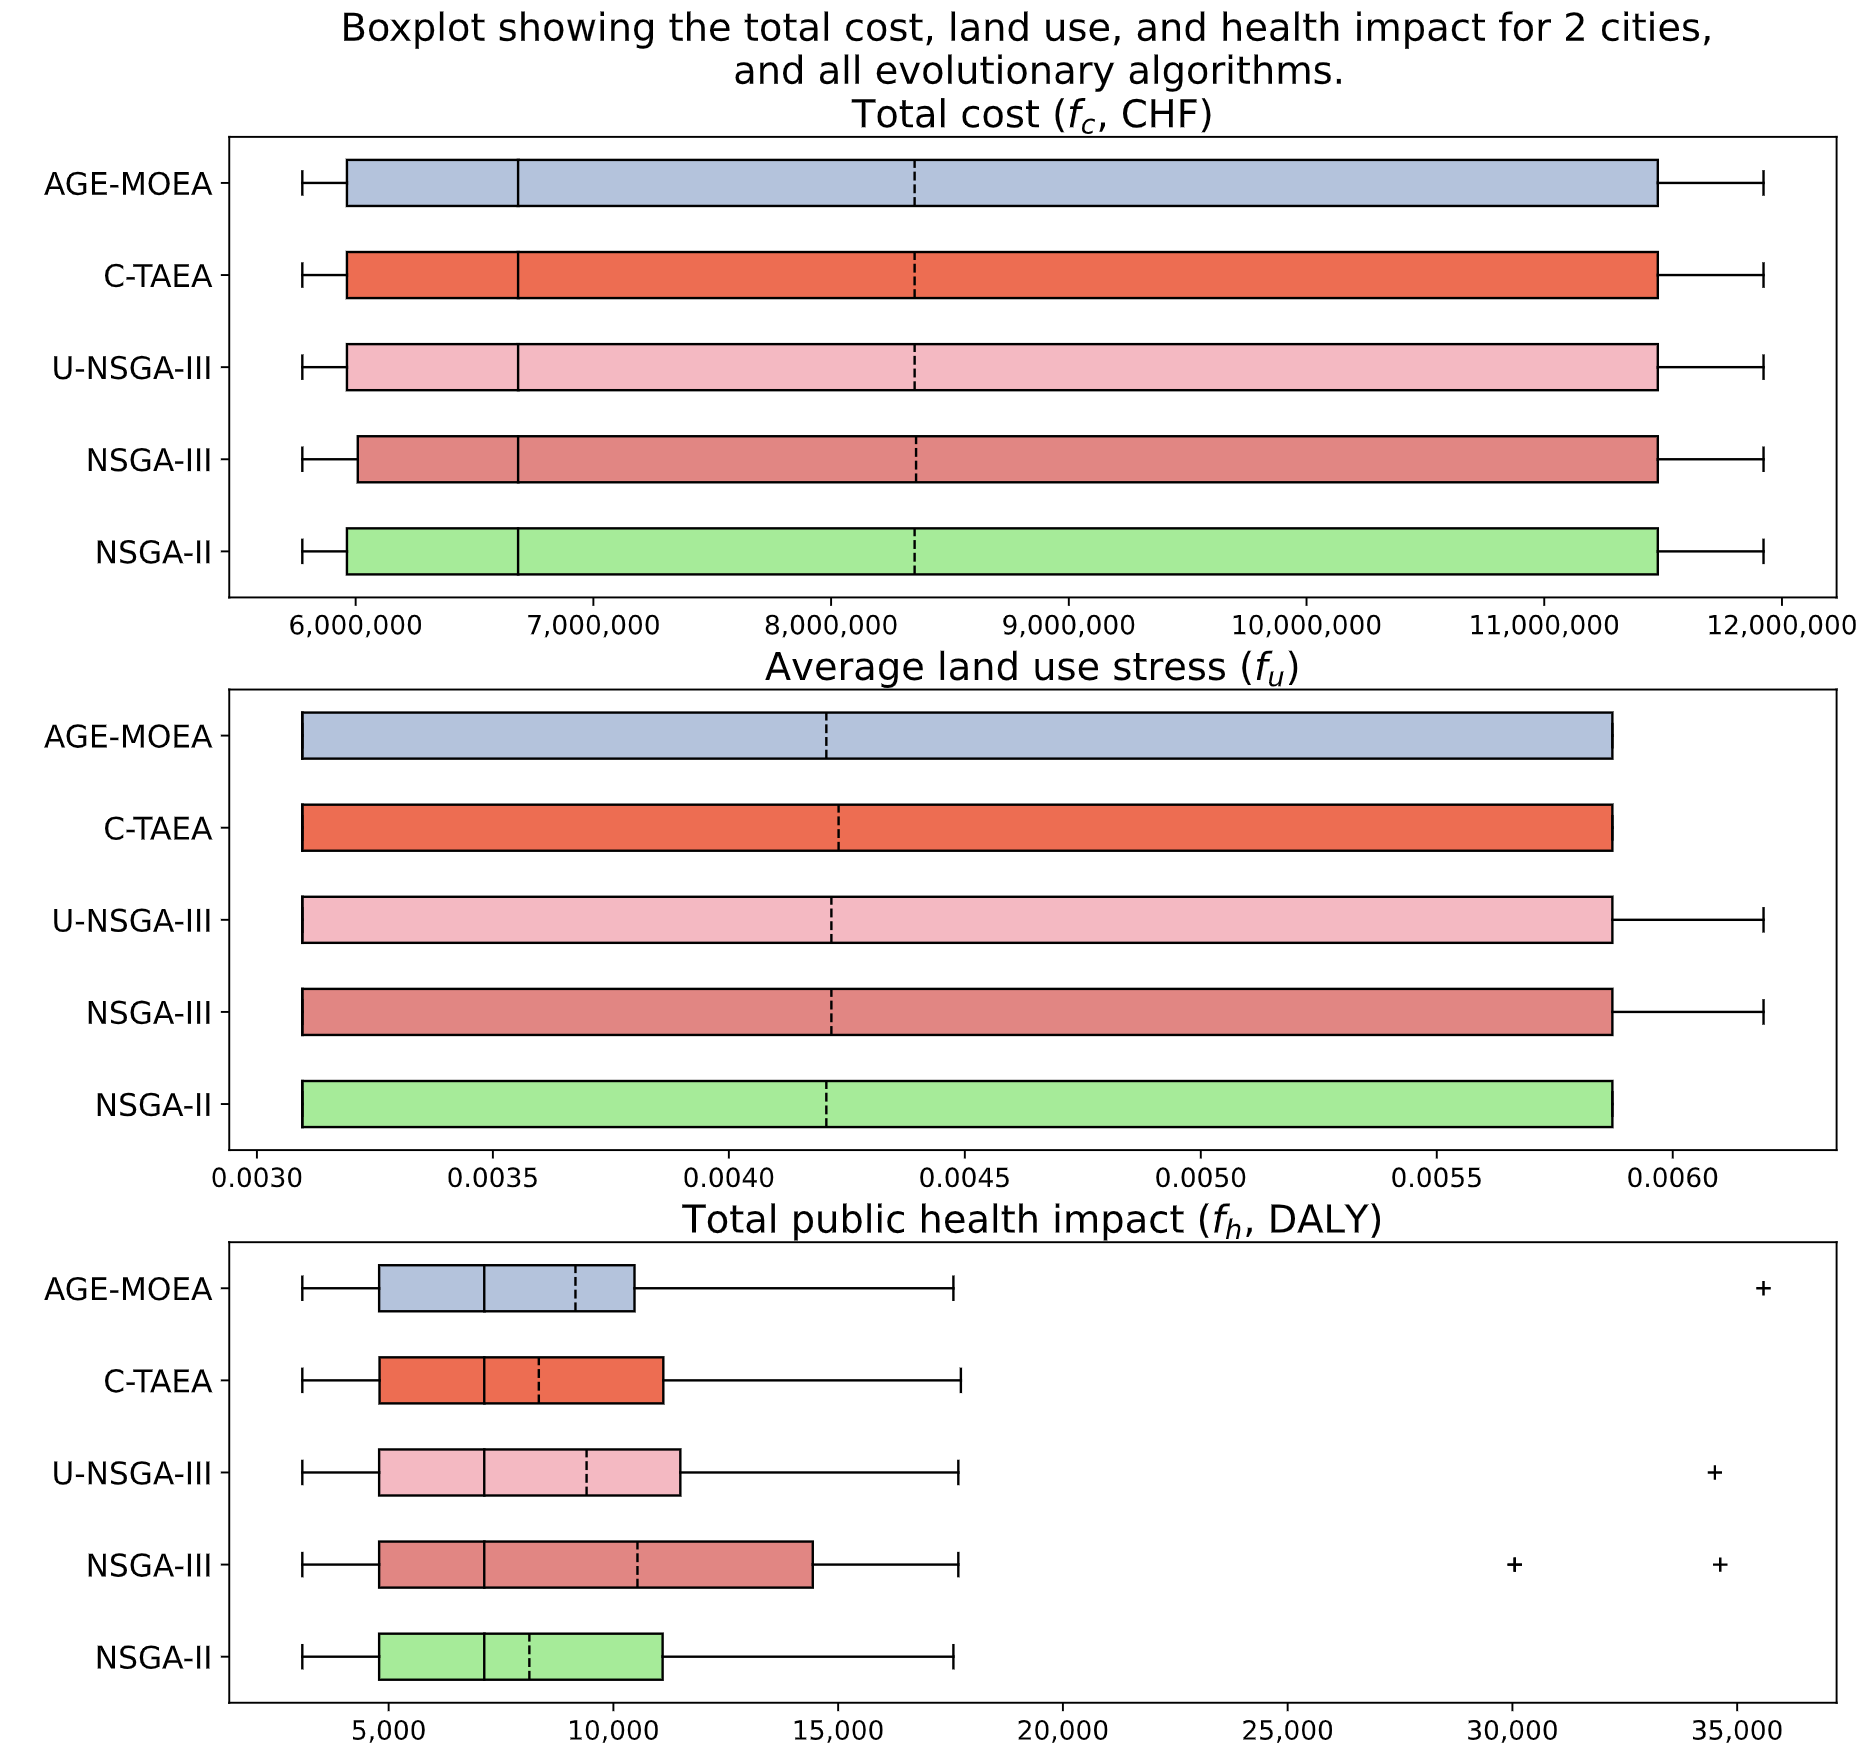
\includegraphics[width=1\textwidth]{/results/boxplots/boxplot_2_cities.png}
    \caption{Boxplot for two cities.}
    \label{fig:2_cities}
\end{subfigure}
\hfill
\begin{subfigure}{0.4\paperwidth}
    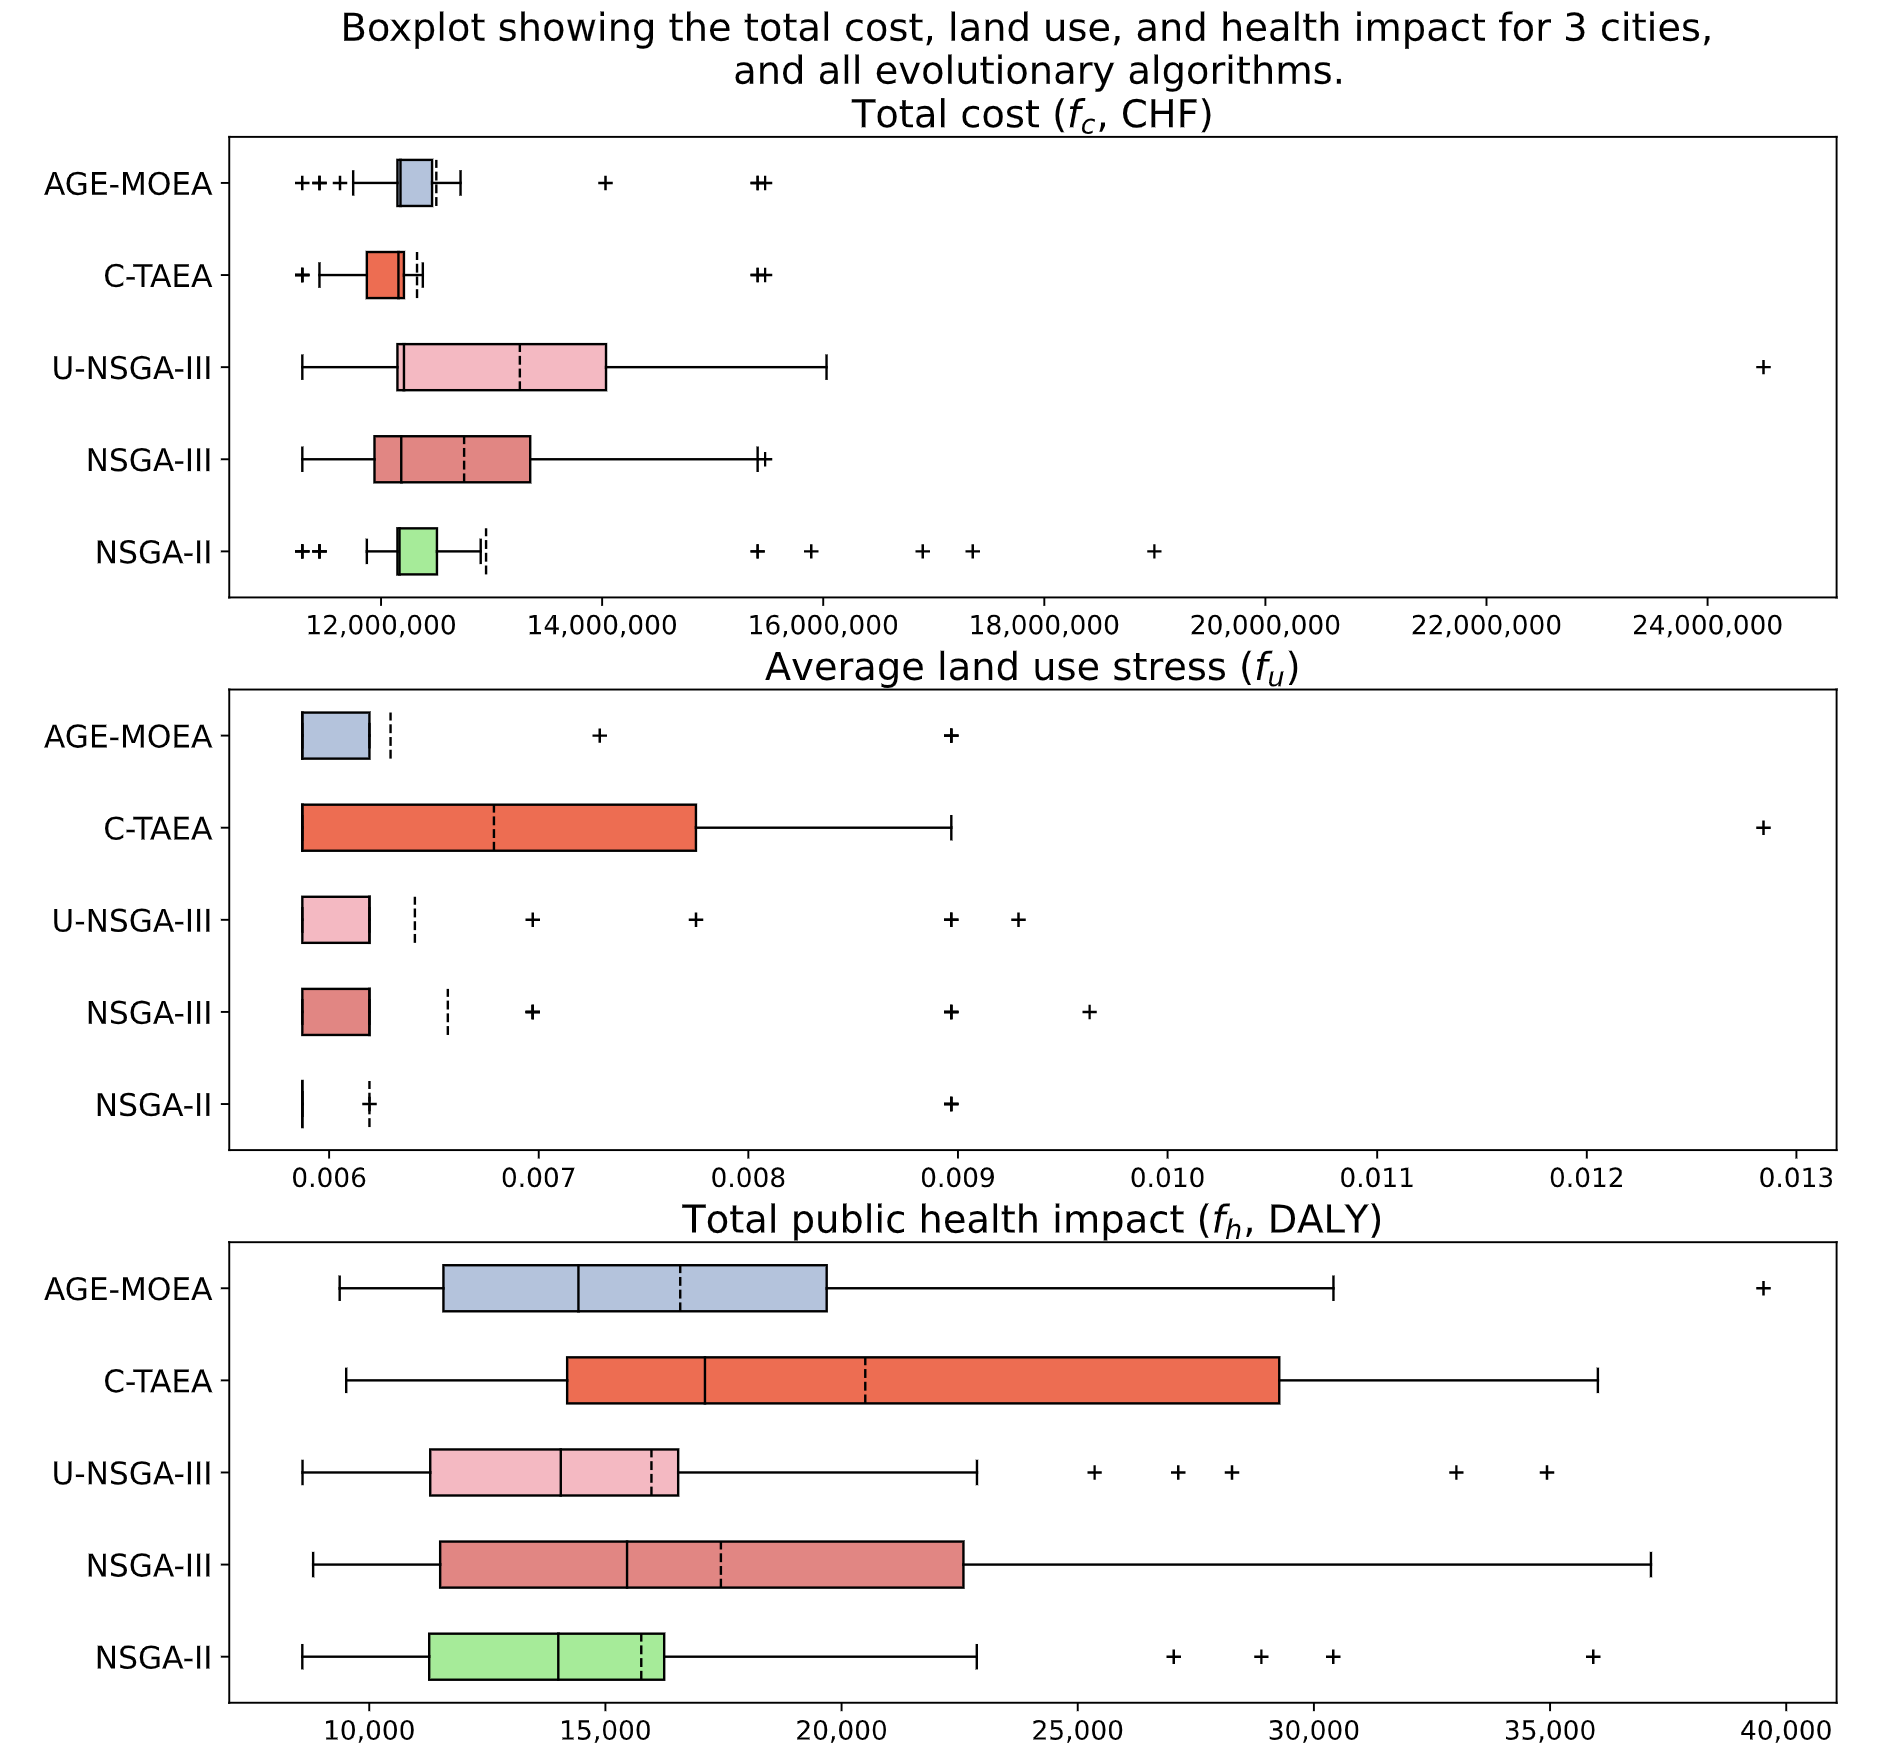
\includegraphics[width=1\textwidth]{/results/boxplots/boxplot_3_cities.png}
    \caption{Boxplot for three cities.}
    \label{fig:3_cities}
\end{subfigure}}
\hfill
\noindent\makebox[\textwidth]{
\begin{subfigure}{0.4\paperwidth}
    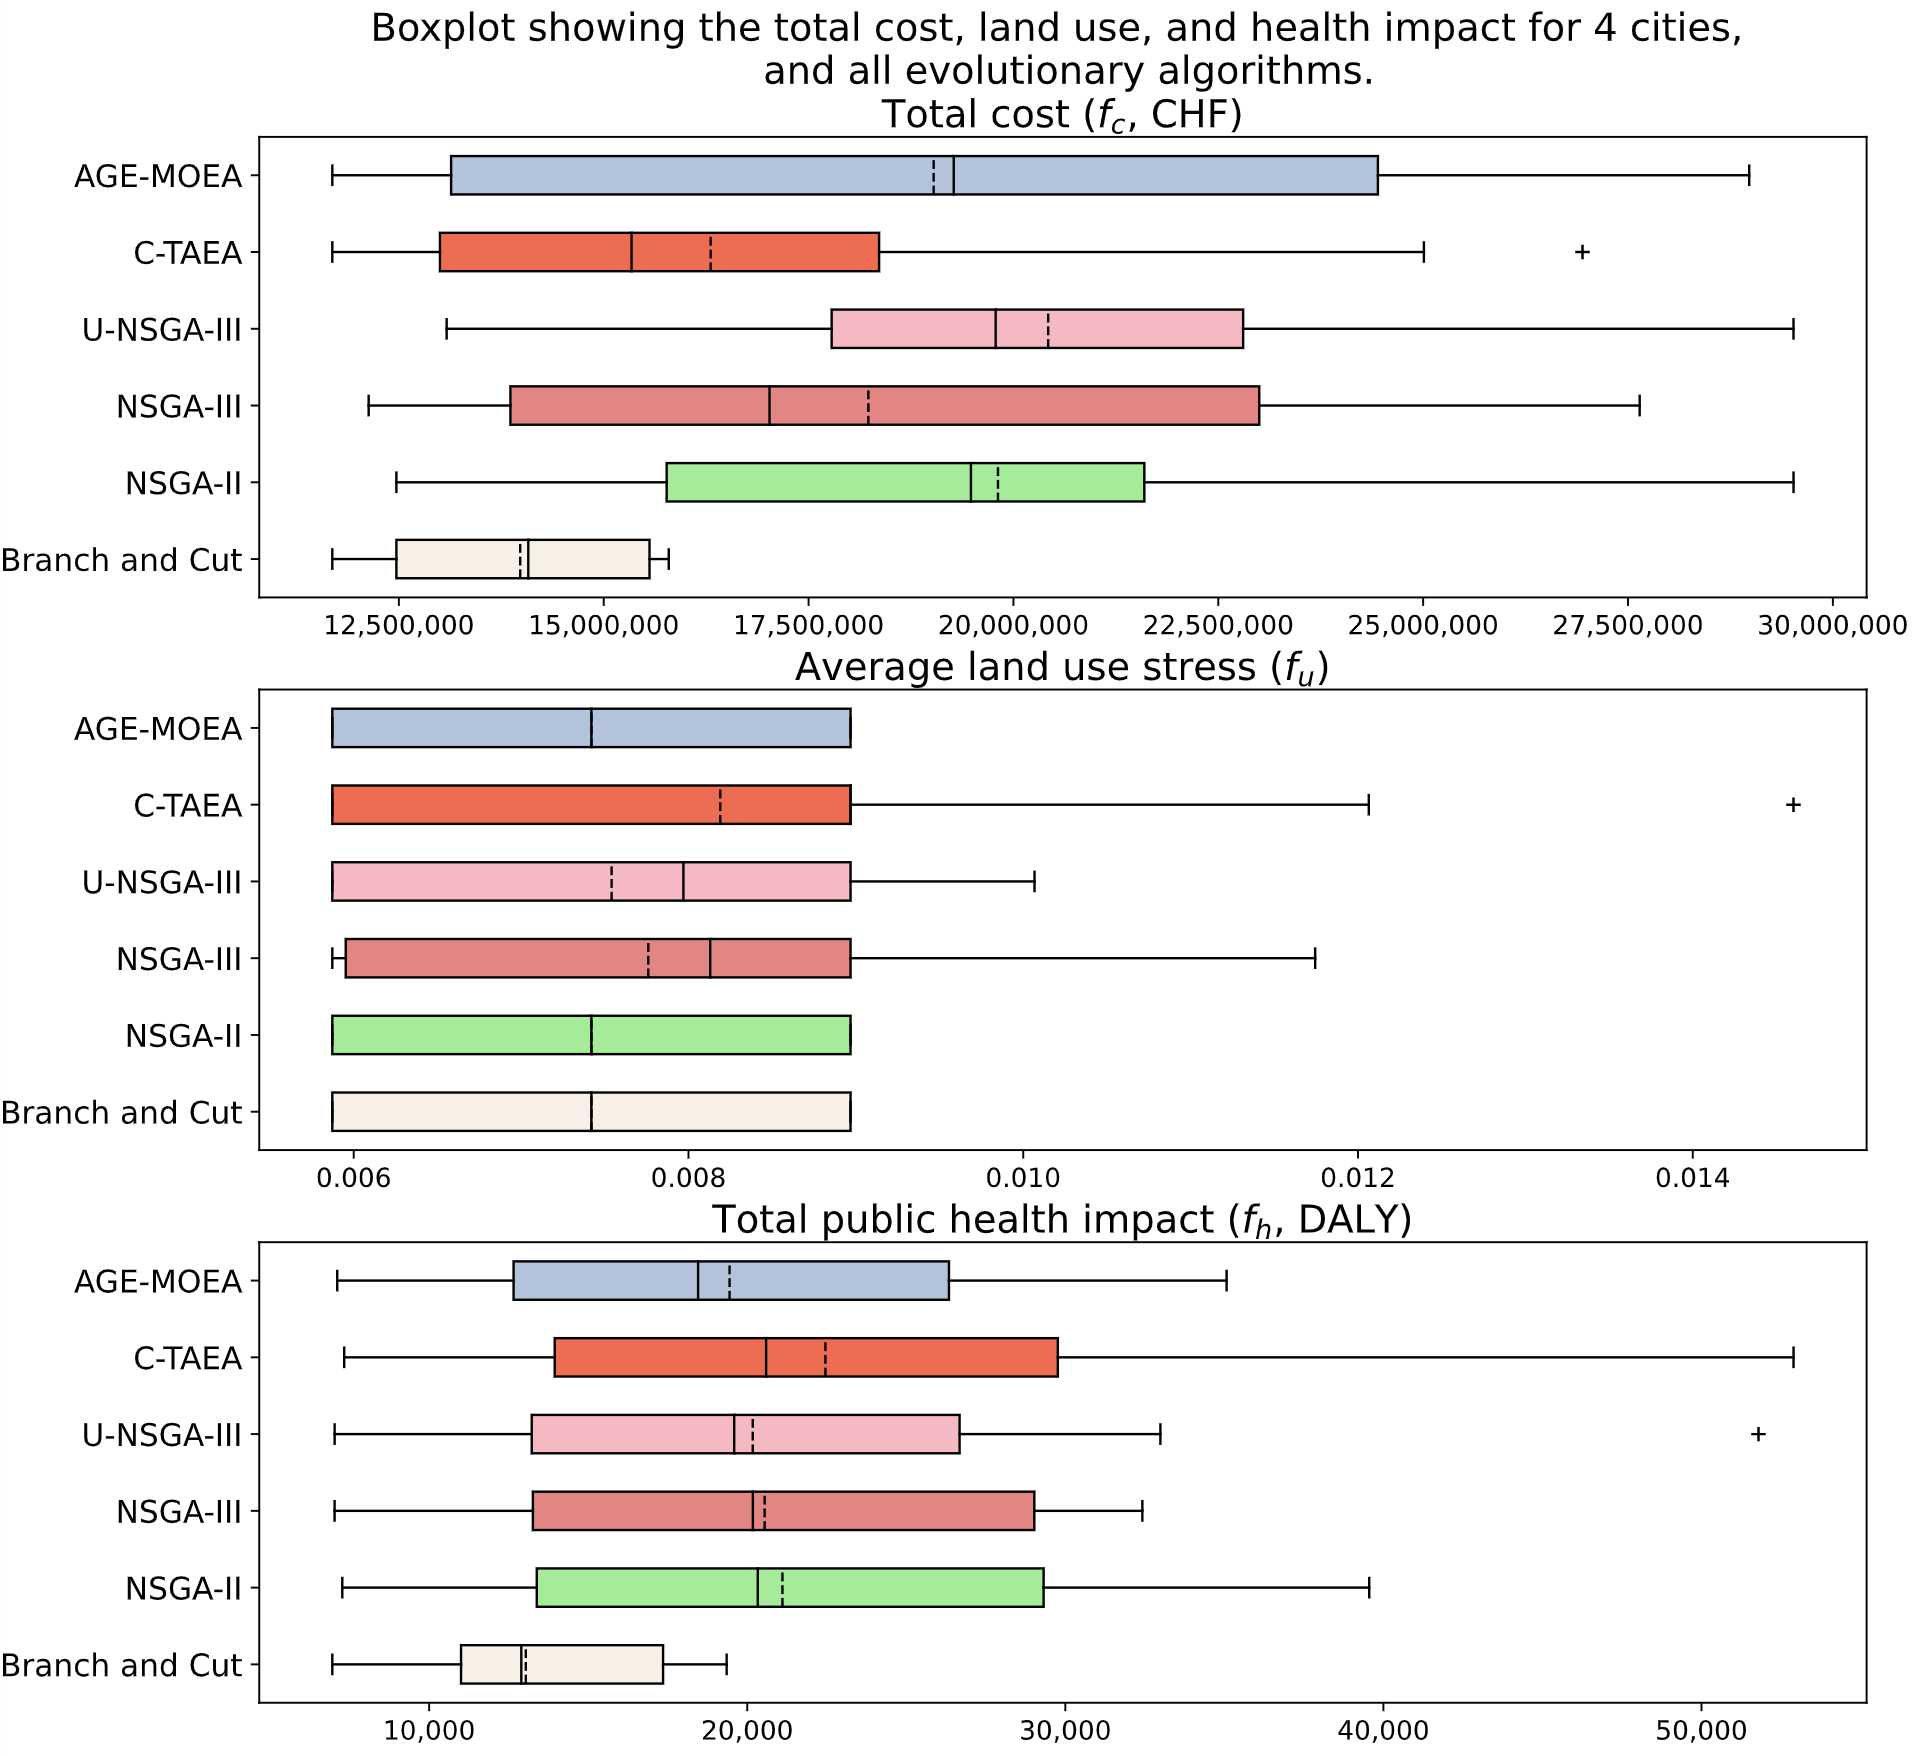
\includegraphics[width=1\textwidth]{/results/boxplots/boxplot_4_cities.png}
    \caption{Boxplot for four cities.}
    \label{fig:4_cities}
\end{subfigure}
\hfill
\begin{subfigure}{0.4\paperwidth}
    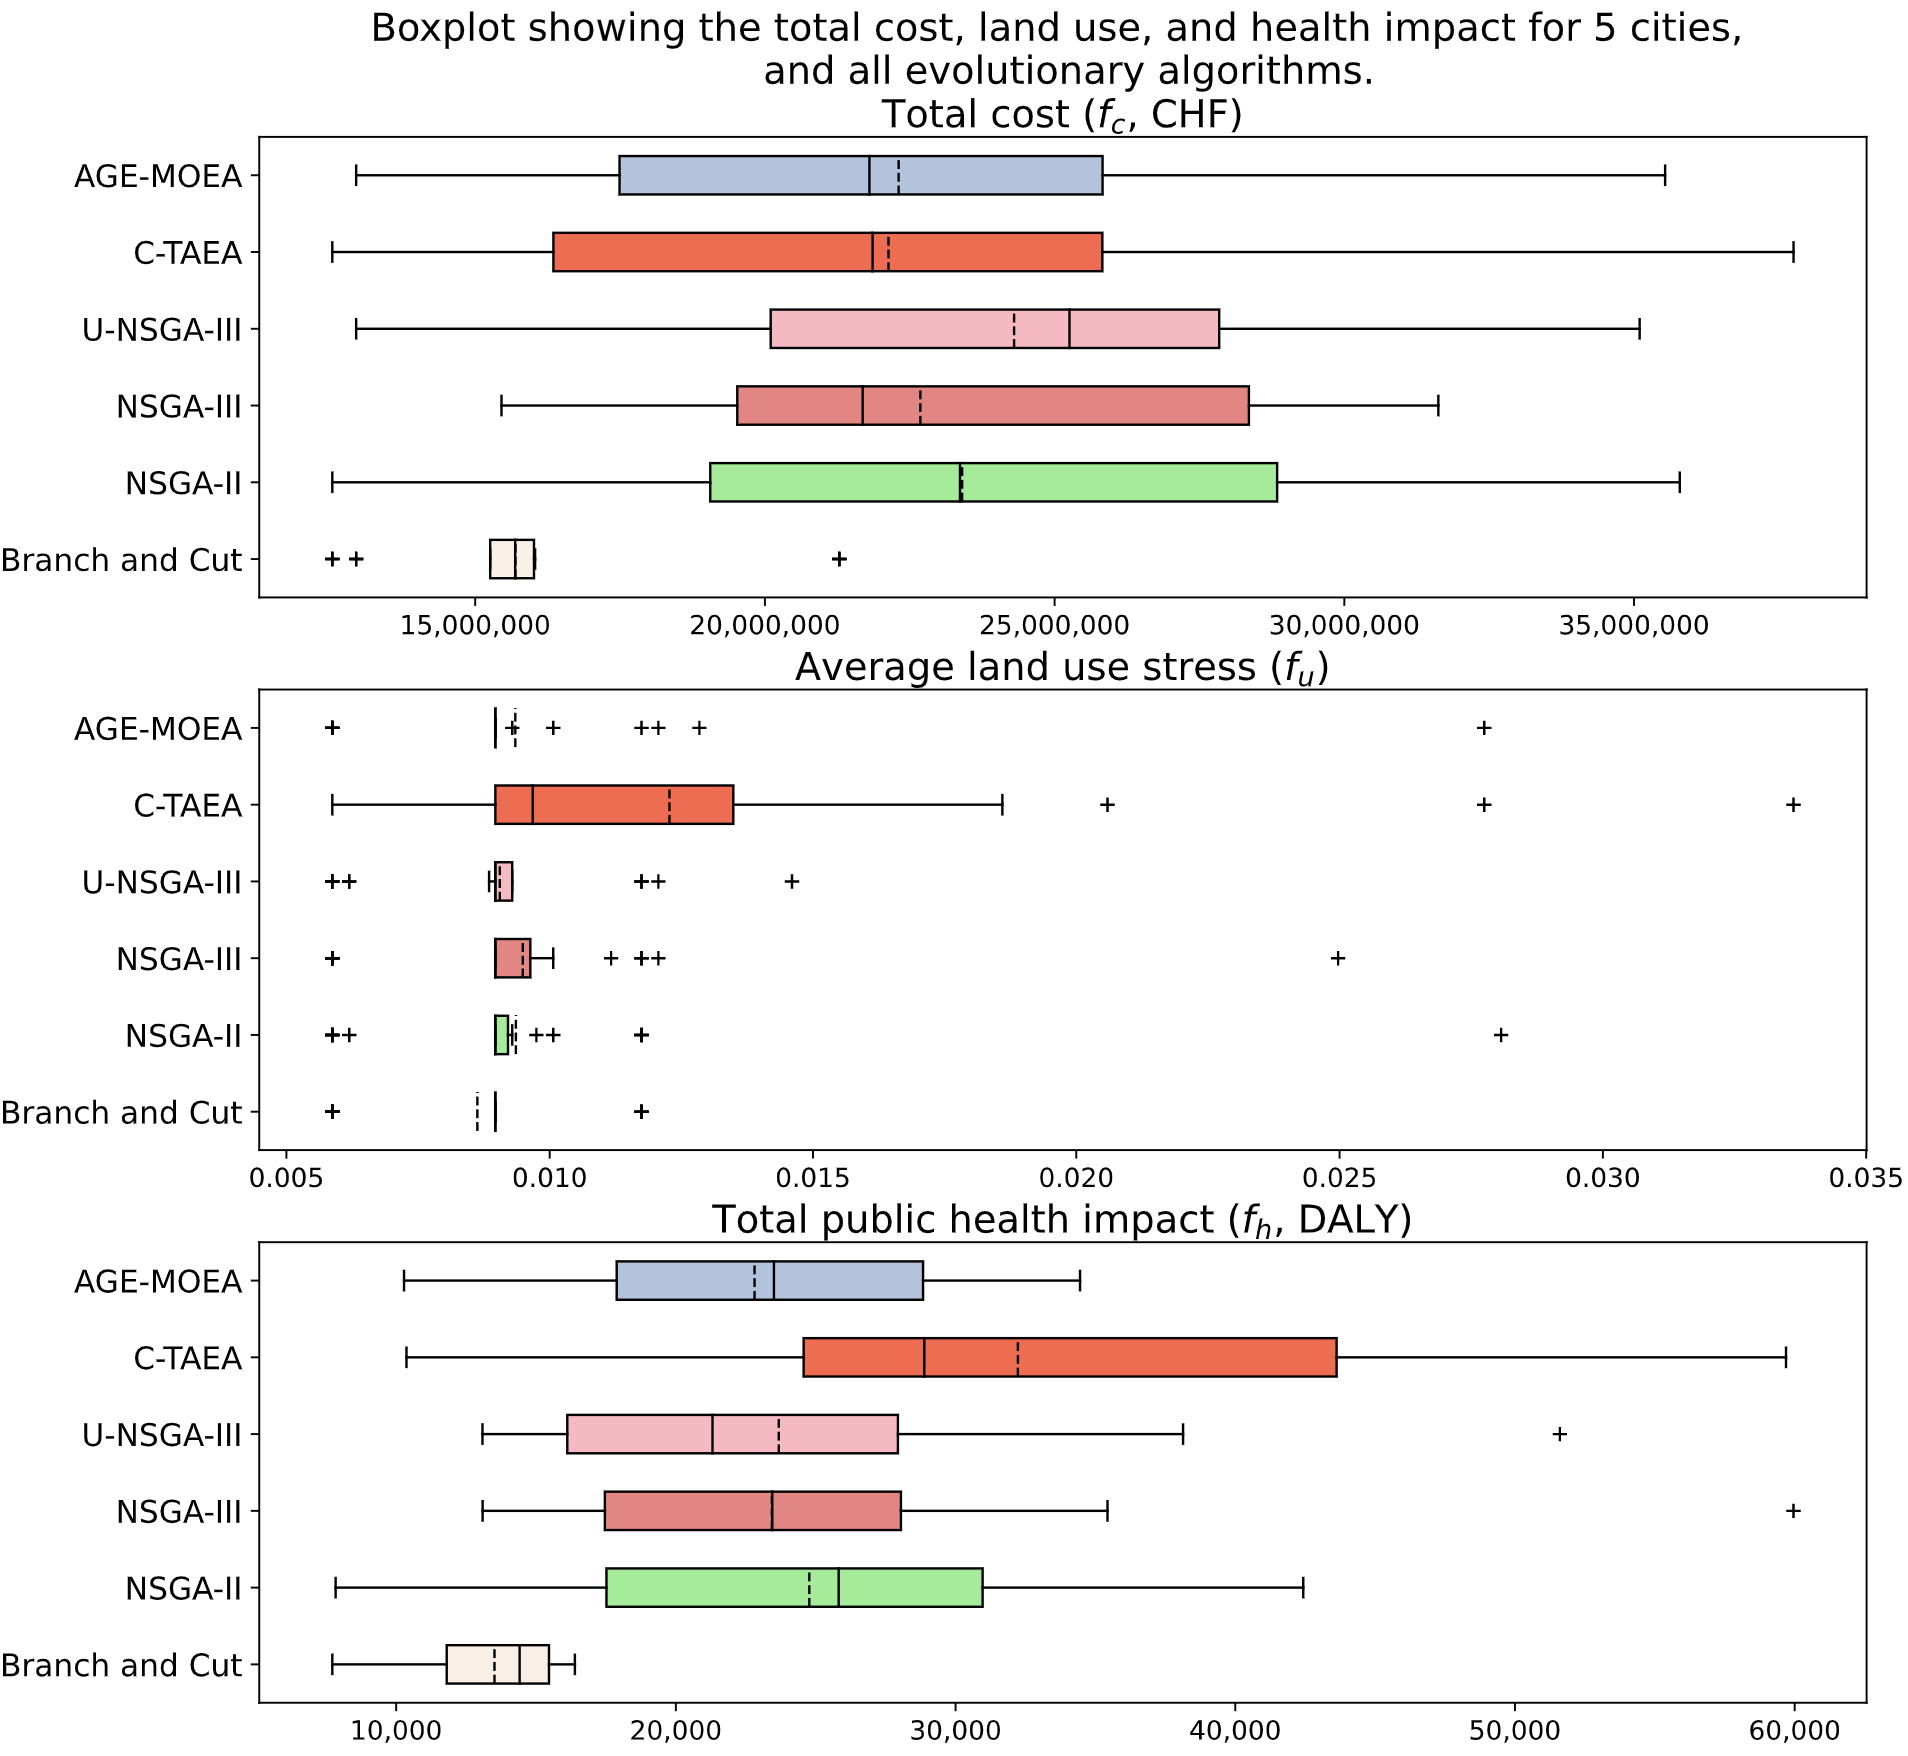
\includegraphics[width=1\textwidth]{/results/boxplots/boxplot_5_cities.png}
    \caption{Boxplot for five cities.}
    \label{fig:5_cities}
\end{subfigure}}
\caption{Boxplots for small-scale problems showing the total cost, land usage stress and health impact for all algorithms.}
\label{fig:boxplot_2_to_5}
\end{figure}

\begin{figure}[ht]
\centering
\noindent\makebox[\textwidth]{
\begin{subfigure}{0.4\paperwidth}

    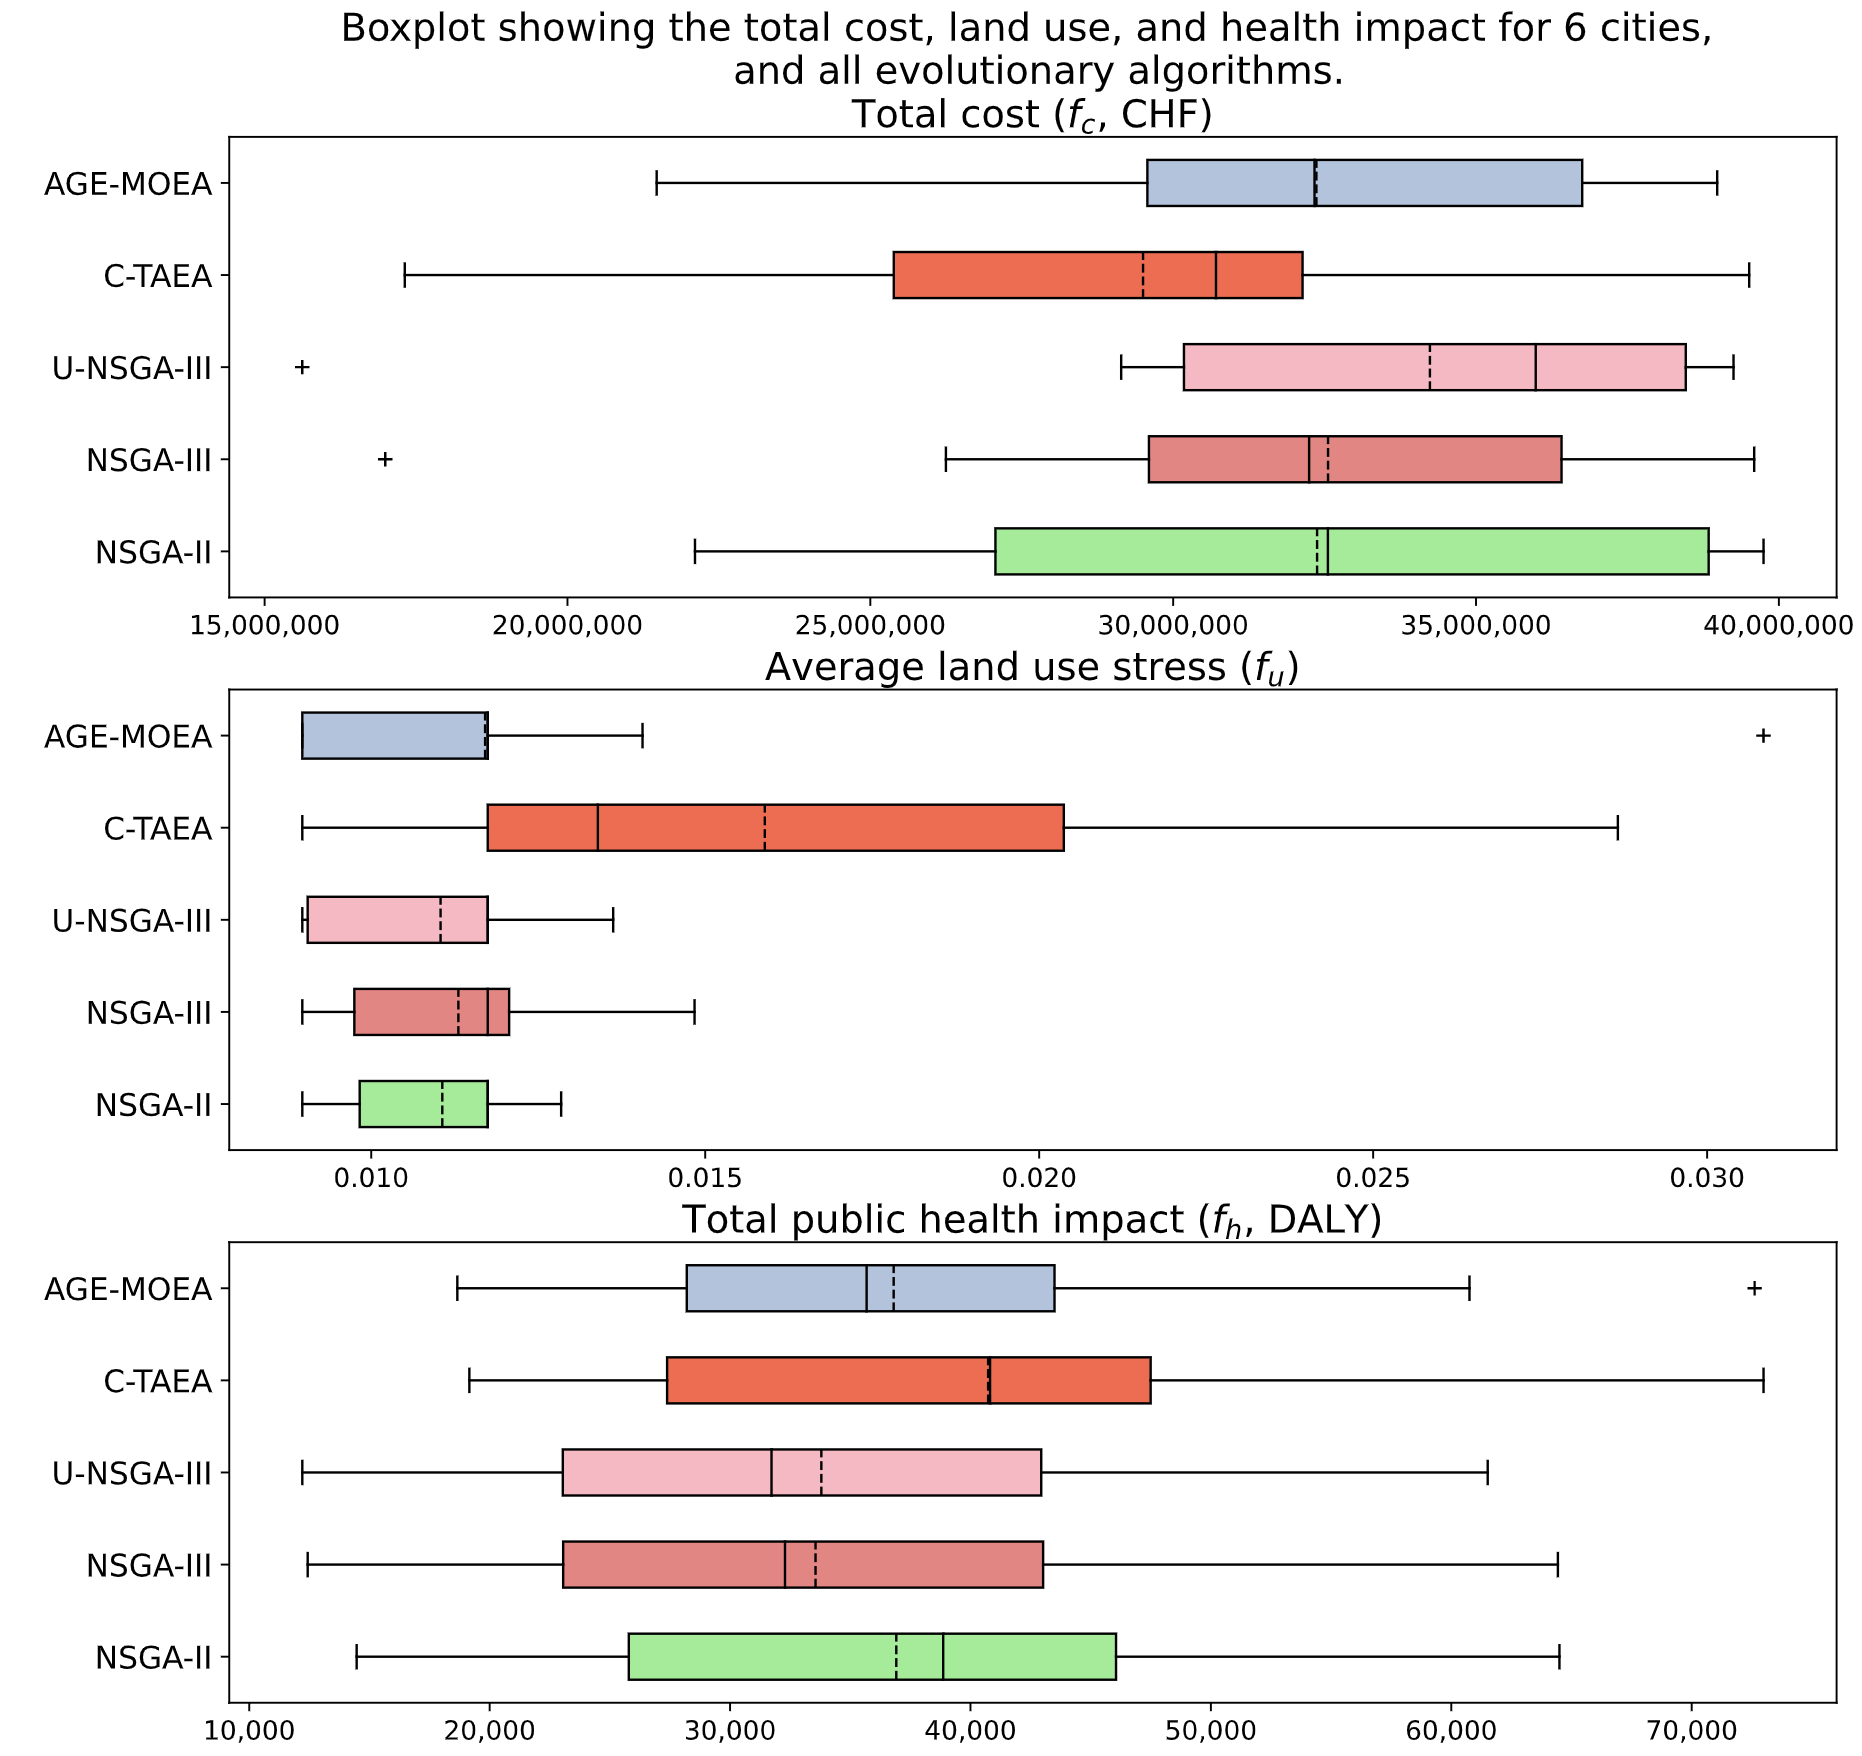
\includegraphics[width=1\textwidth]{/results/boxplots/boxplot_6_cities.png}
    \caption{Boxplot for six cities.}
    \label{fig:6_cities}
\end{subfigure}
\hfill
\begin{subfigure}{0.4\paperwidth}
    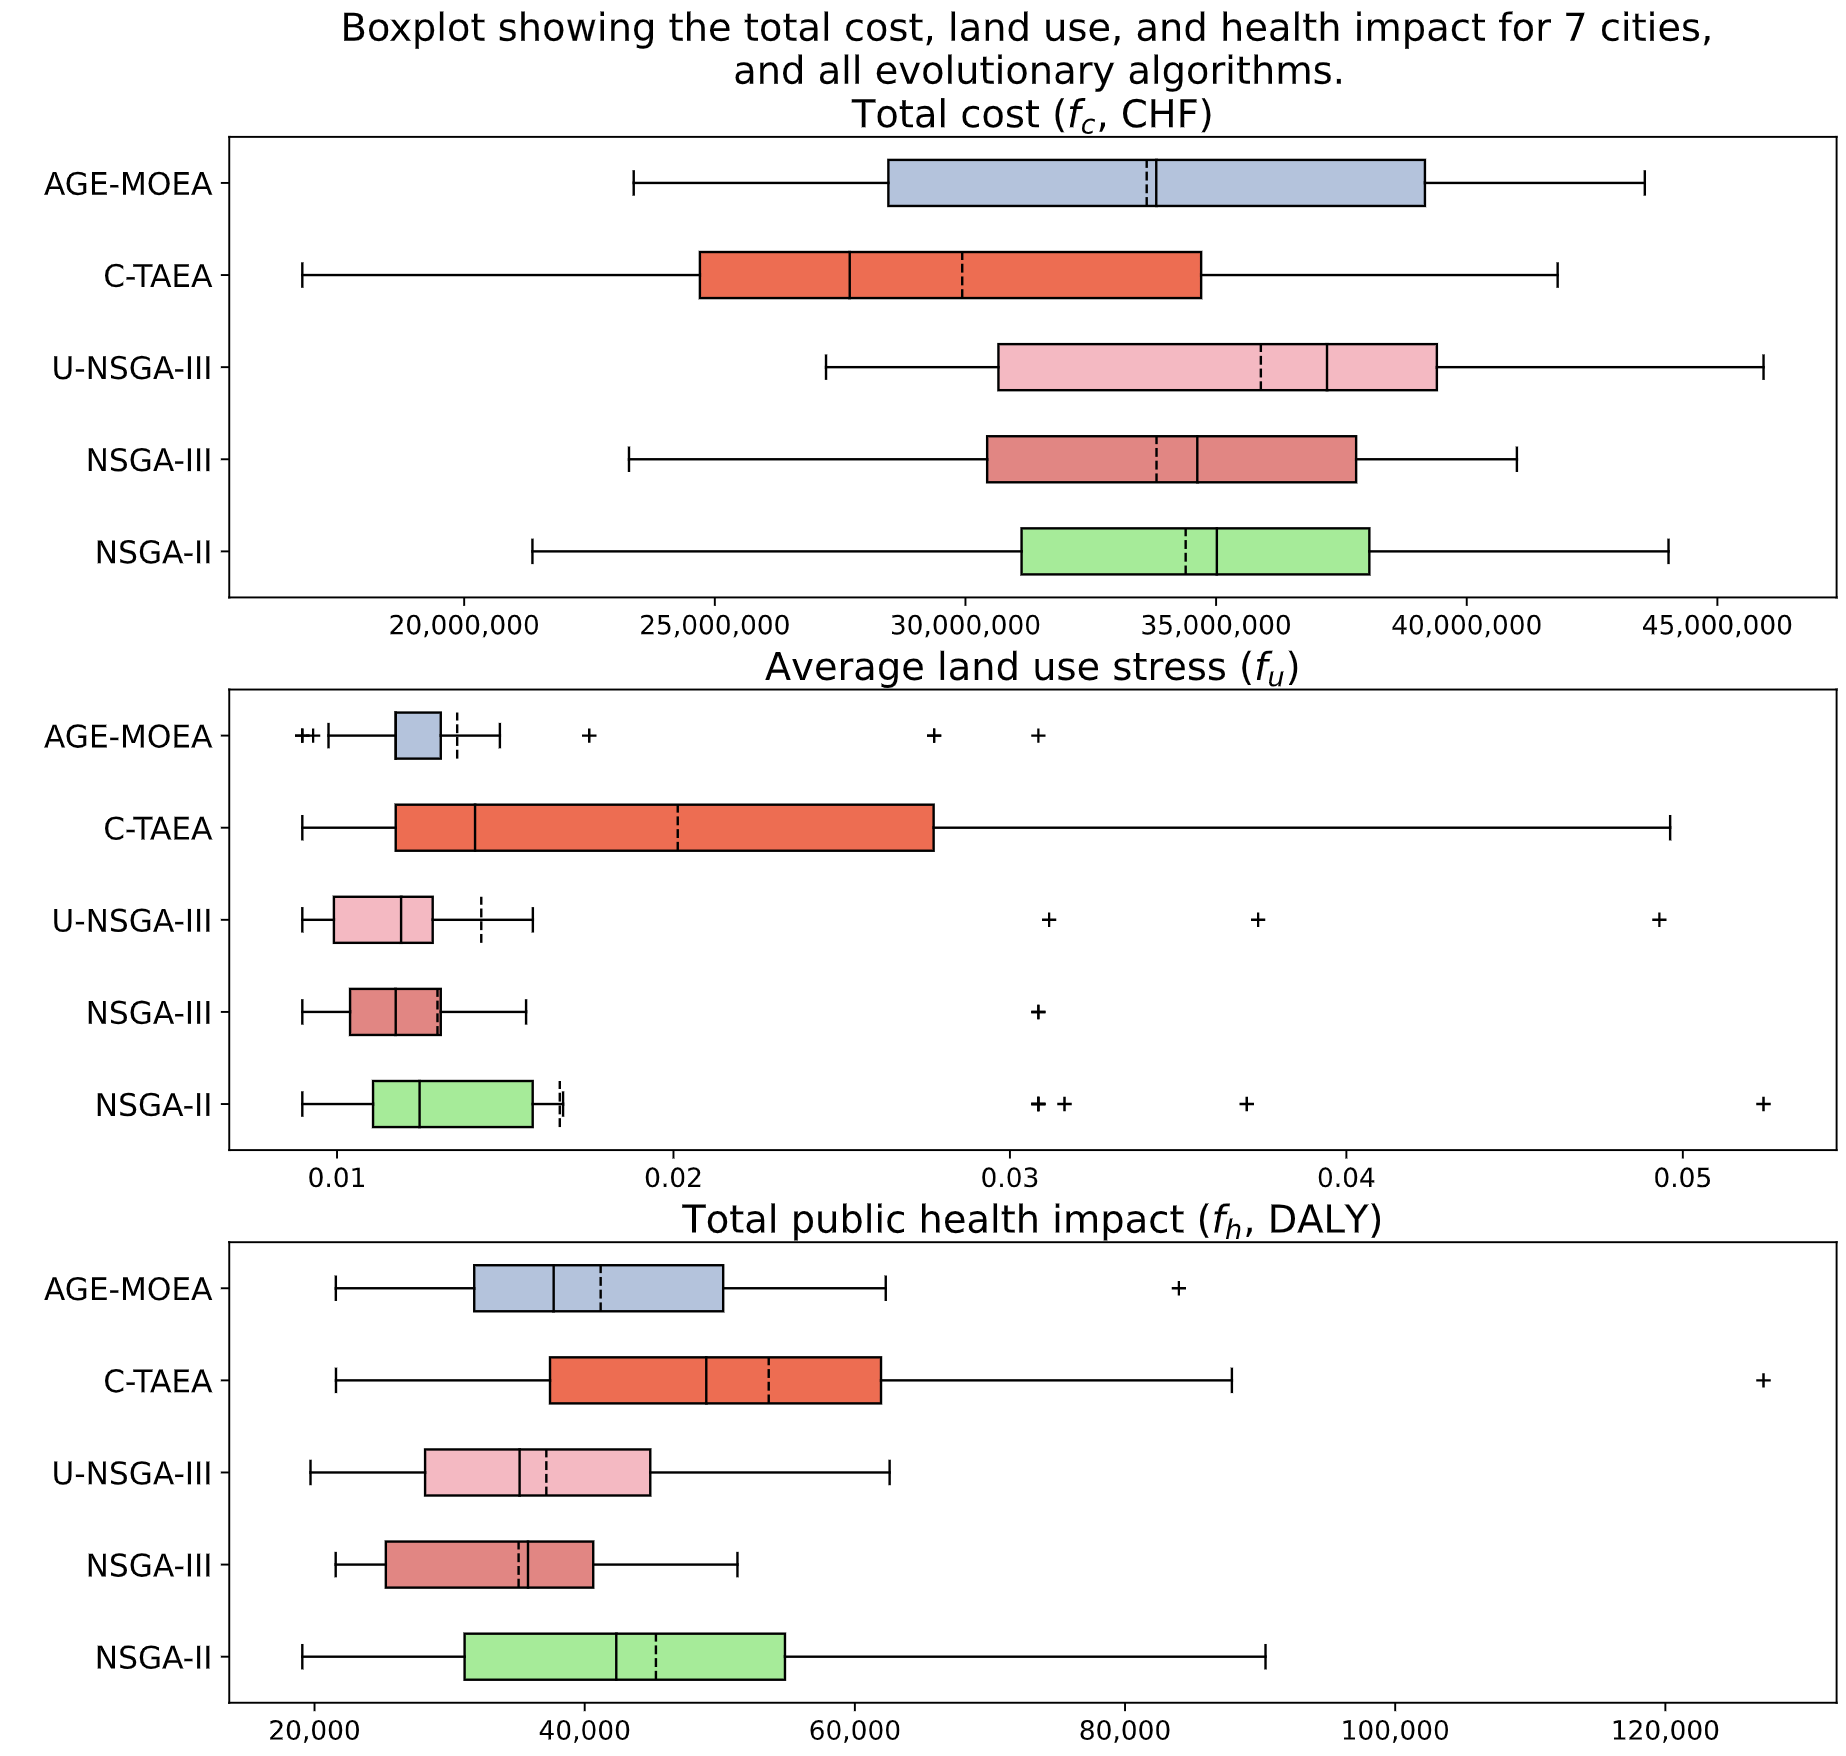
\includegraphics[width=1\textwidth]{/results/boxplots/boxplot_7_cities.png}
    \caption{Boxplot for seven cities.}
    \label{fig:7_cities}
\end{subfigure}}
\hfill
\noindent\makebox[\textwidth]{
\begin{subfigure}{0.4\paperwidth}
    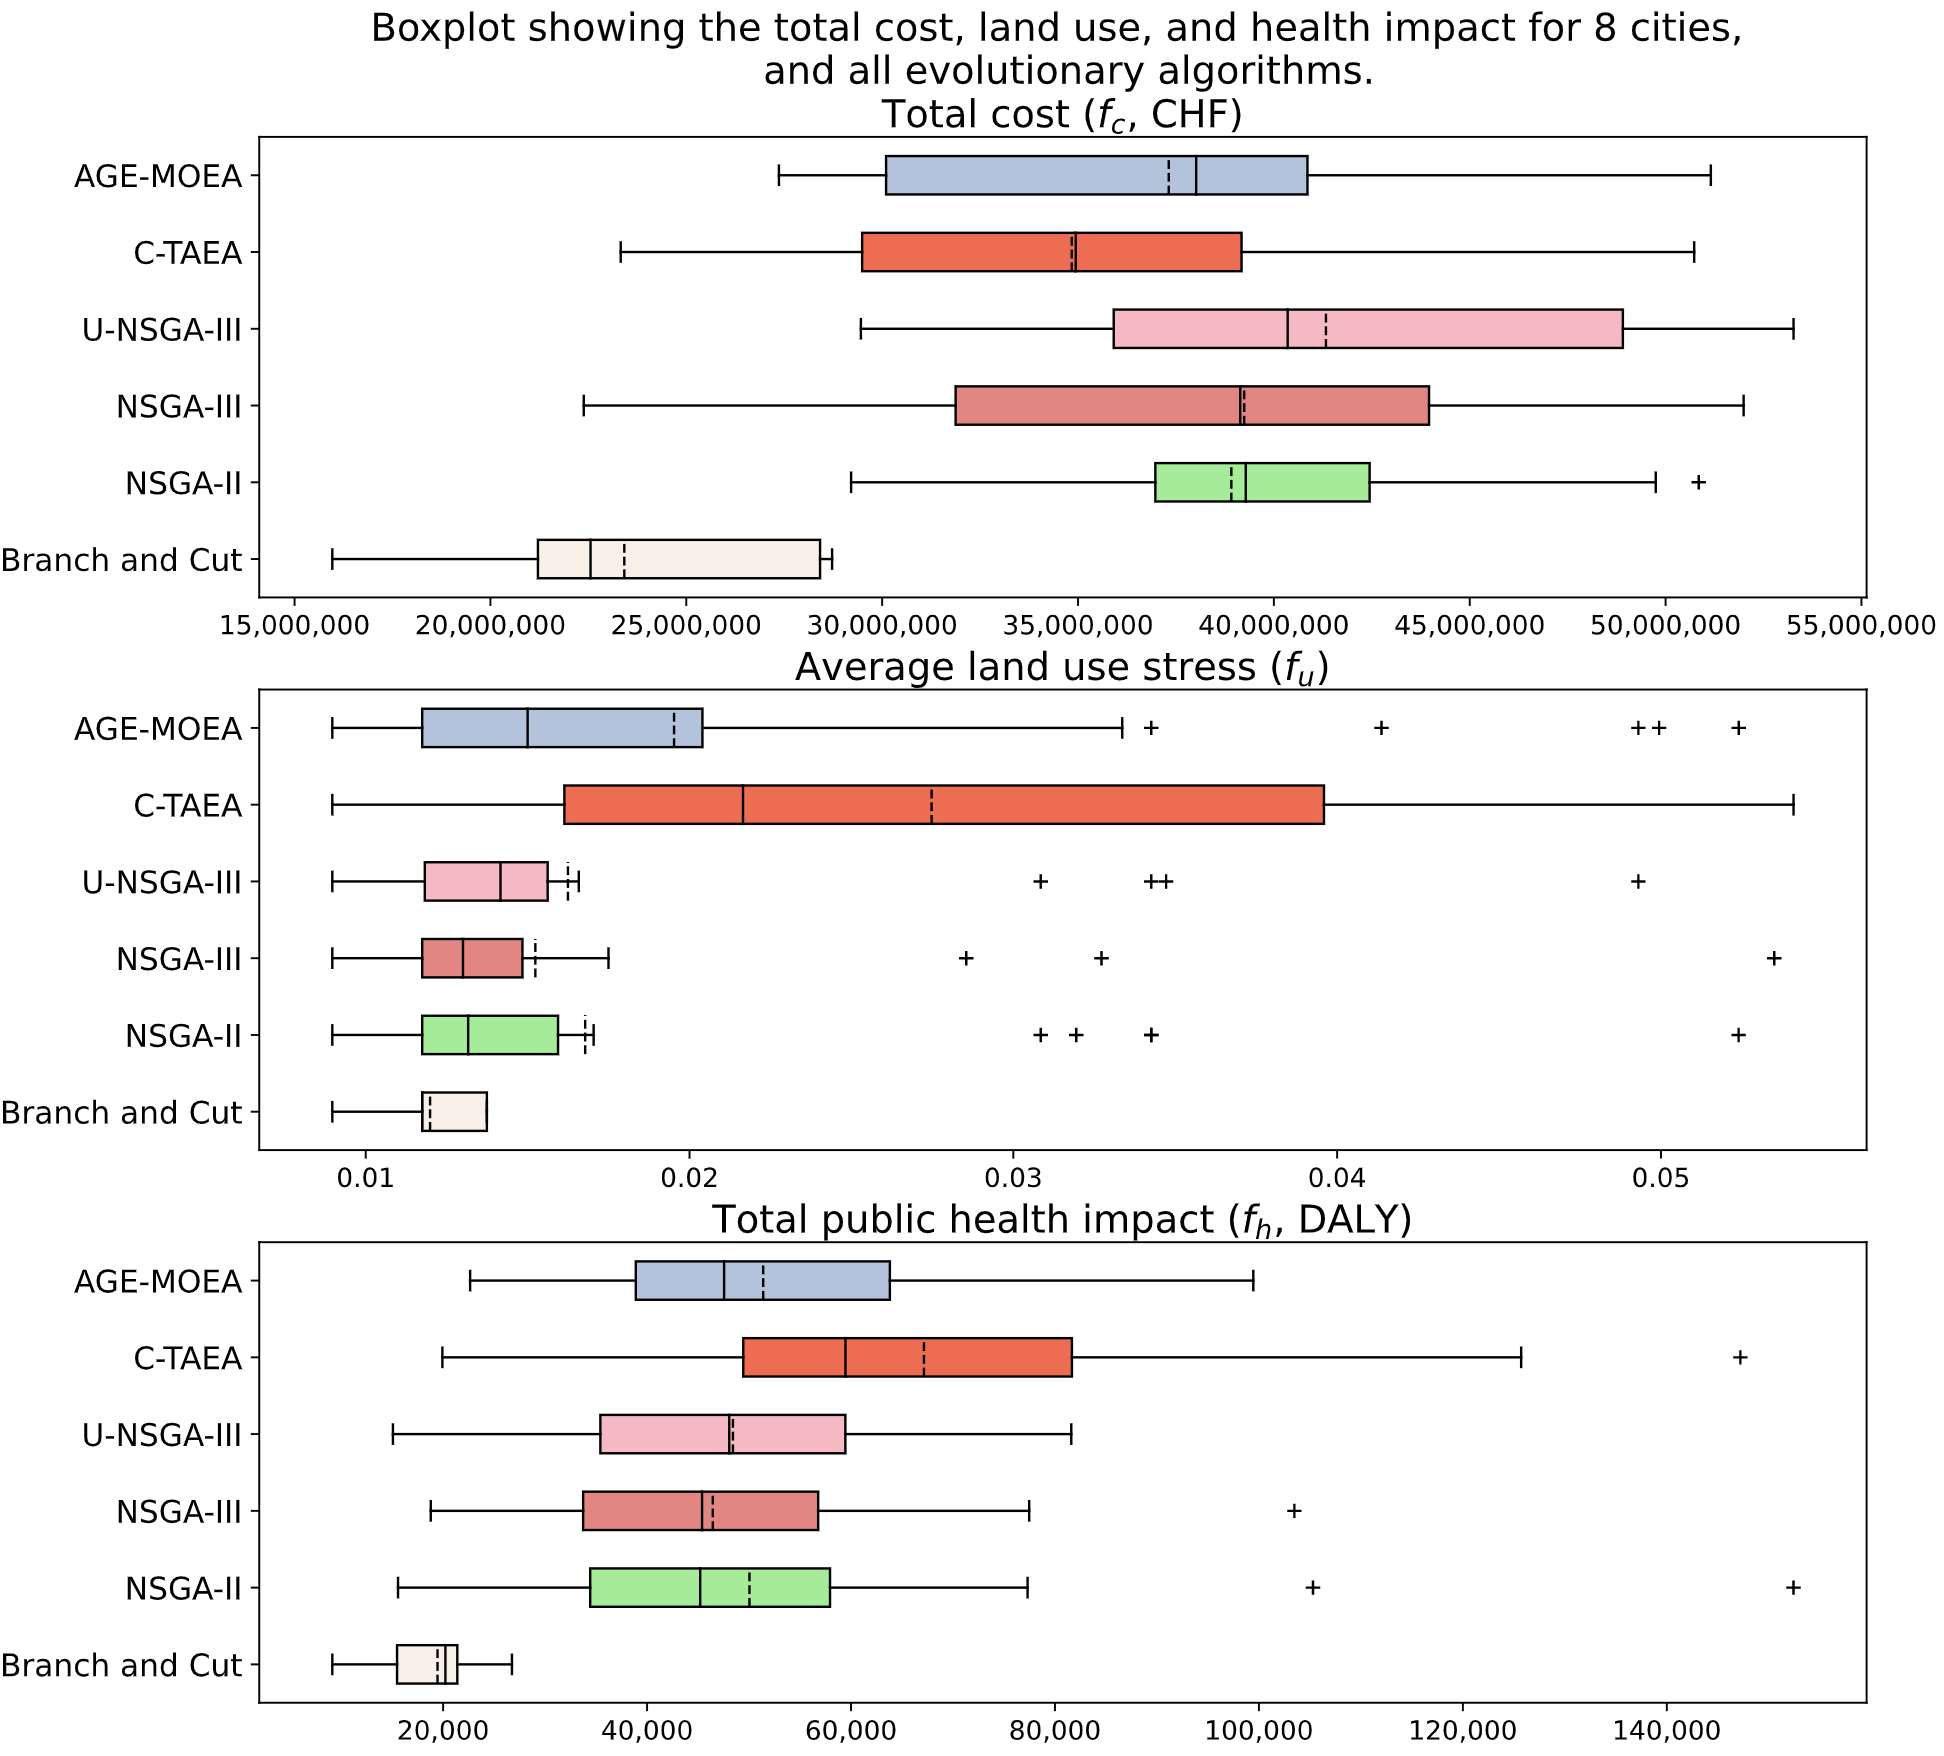
\includegraphics[width=1\textwidth]{/results/boxplots/boxplot_8_cities.png}
    \caption{Boxplot for eight cities.}
    \label{fig:8_cities}
\end{subfigure}
\hfill
\begin{subfigure}{0.4\paperwidth}
    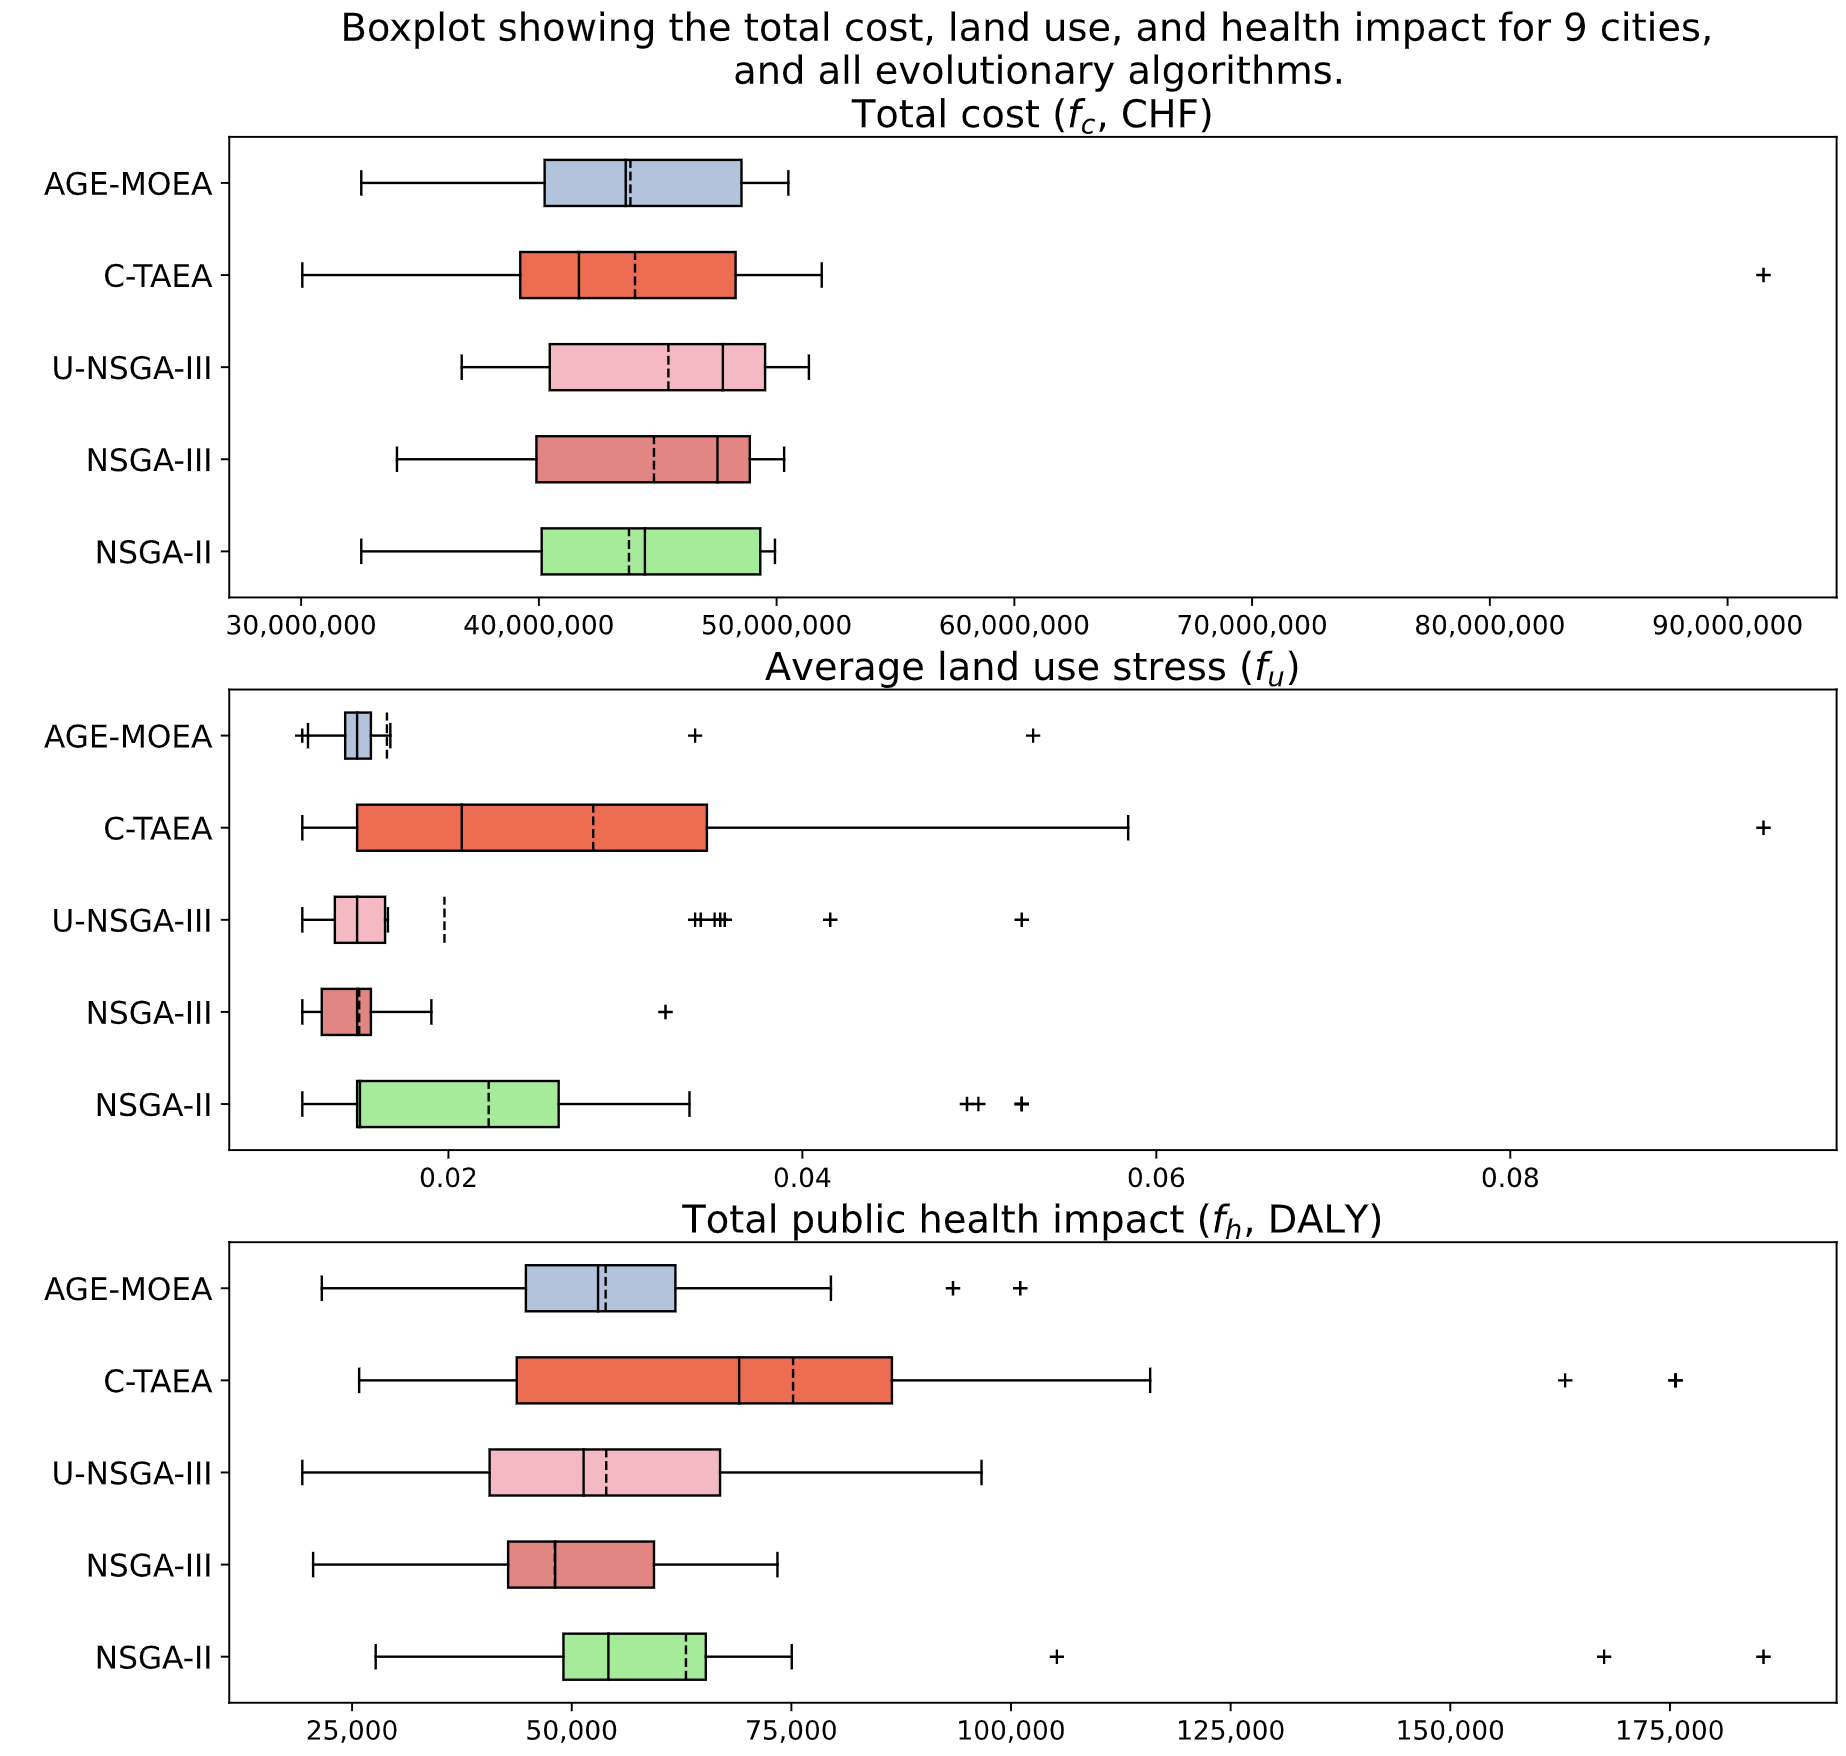
\includegraphics[width=1\textwidth]{/results/boxplots/boxplot_9_cities.png}
    \caption{Boxplot for nine cities.}
    \label{fig:9_cities}
\end{subfigure}}
\hfill
\begin{subfigure}{0.4\paperwidth}
    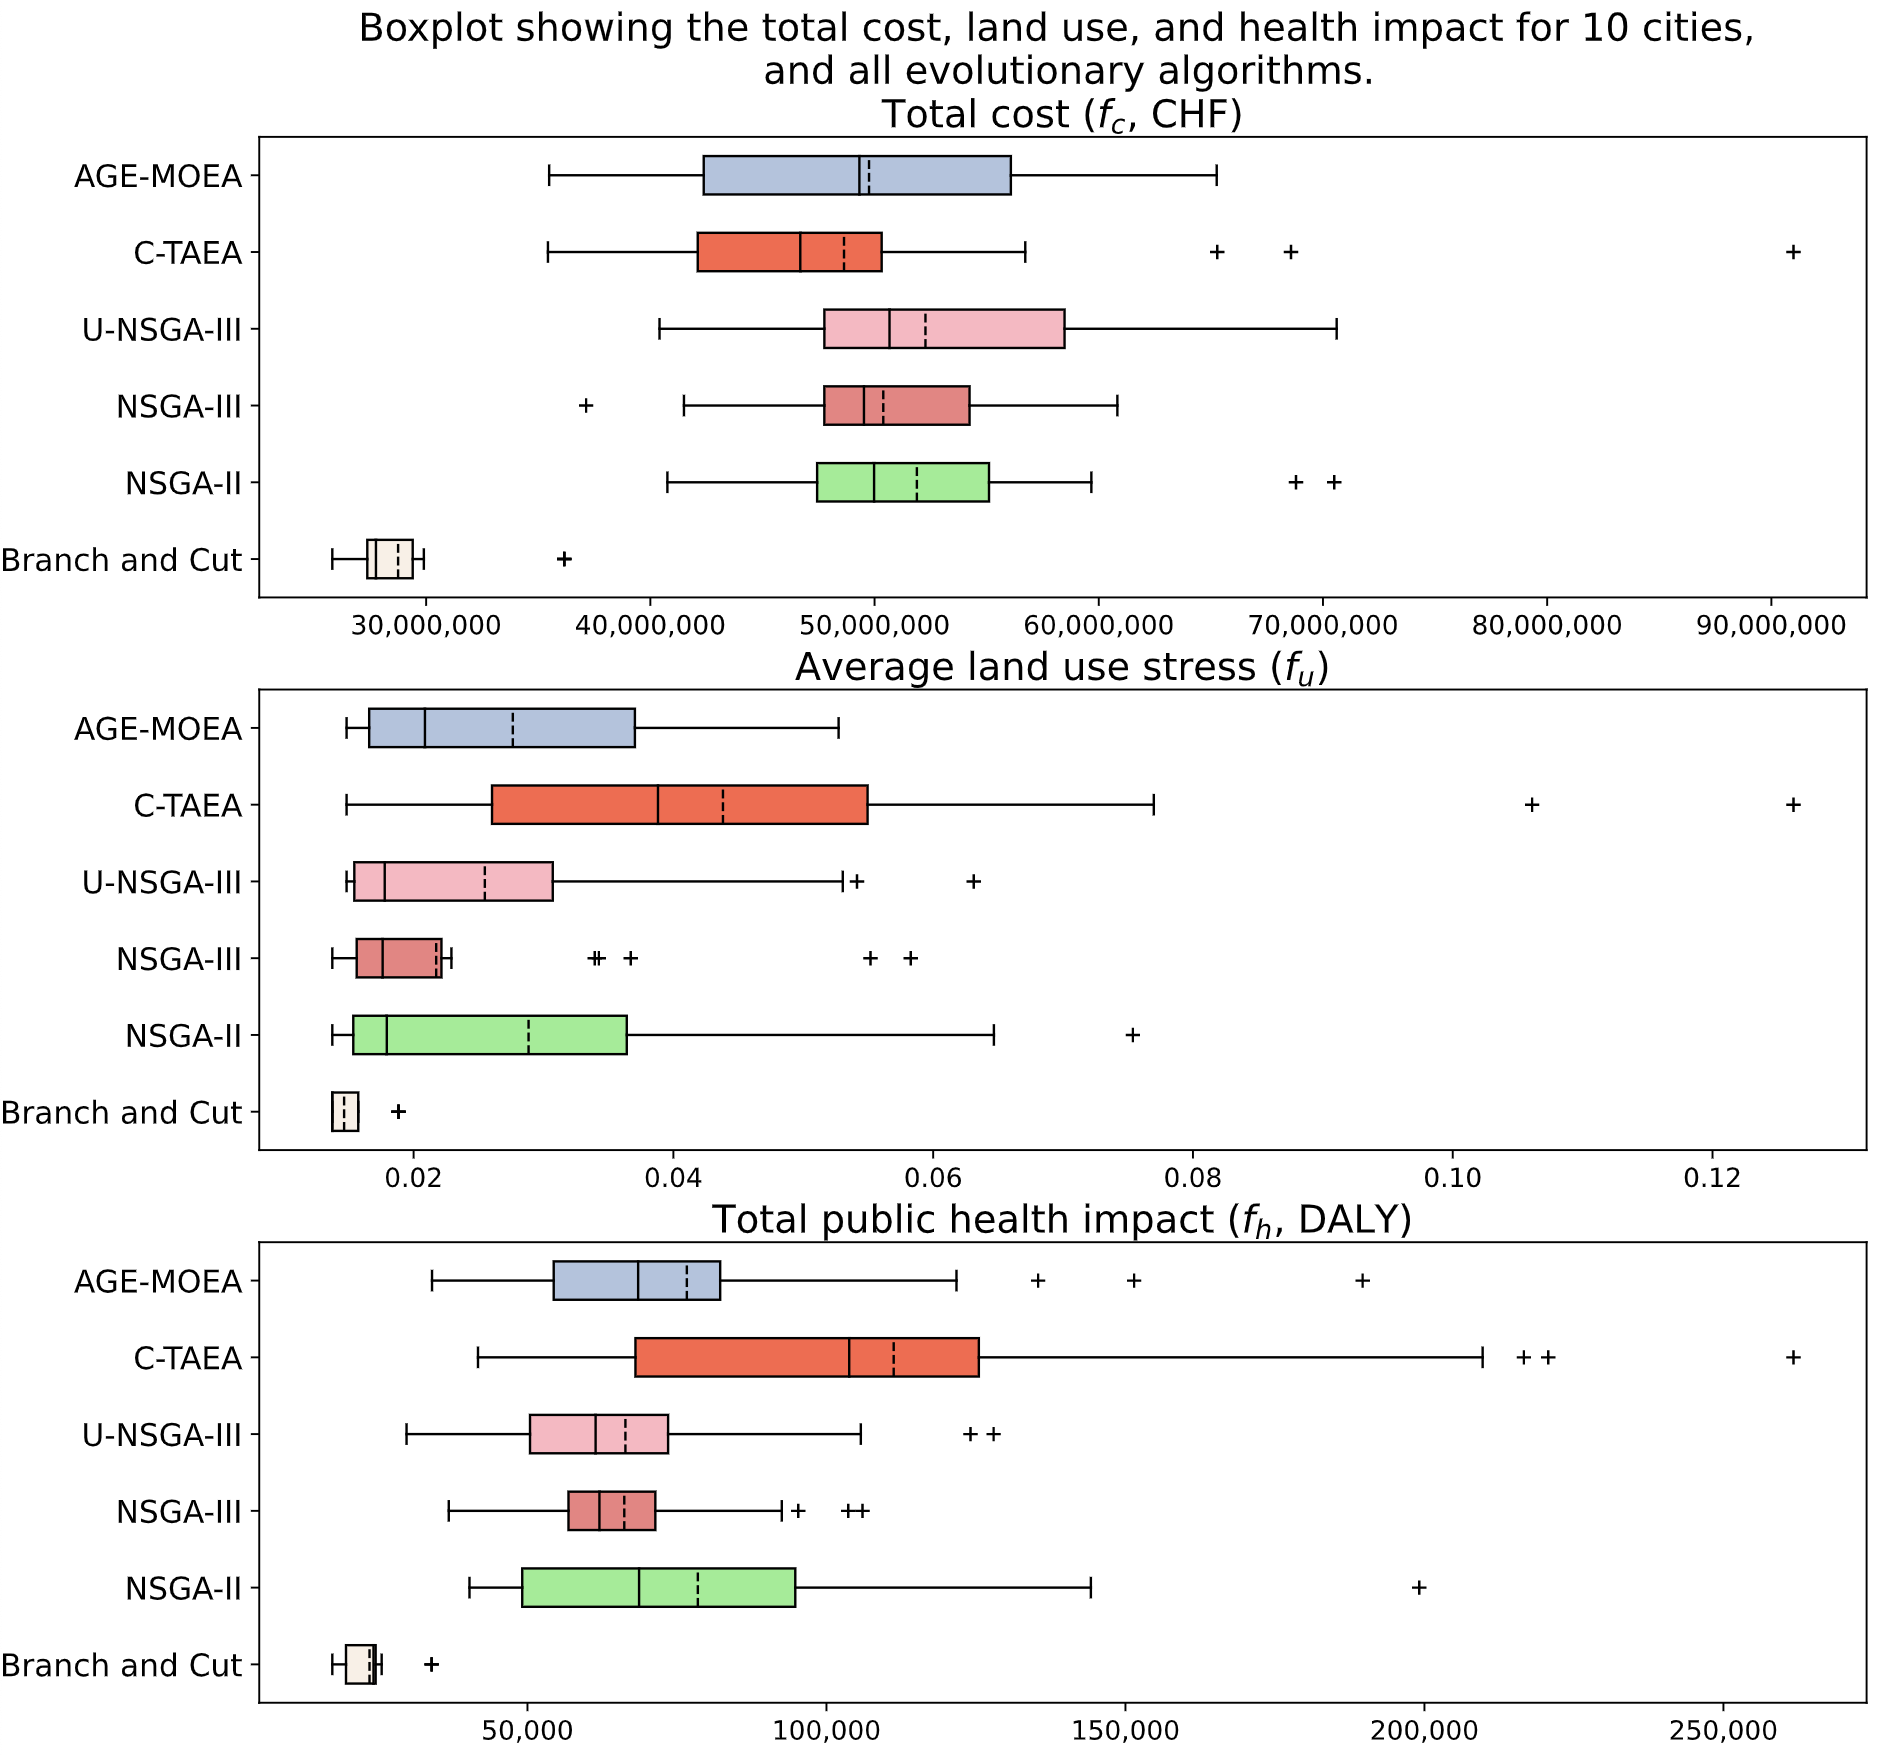
\includegraphics[width=1\textwidth]{/results/boxplots/boxplot_10_cities.png}
    \caption{Boxplot for ten cities.}
    \label{fig:10_cities}
\end{subfigure}
\caption{Boxplots for medium-sized problems showing the total cost, land usage stress and health impact for all algorithms.}
\label{fig:boxplot_6_to_10}
\end{figure}

\begin{figure}[ht]
\centering
\noindent\makebox[\textwidth]{
\begin{subfigure}{0.4\paperwidth}

    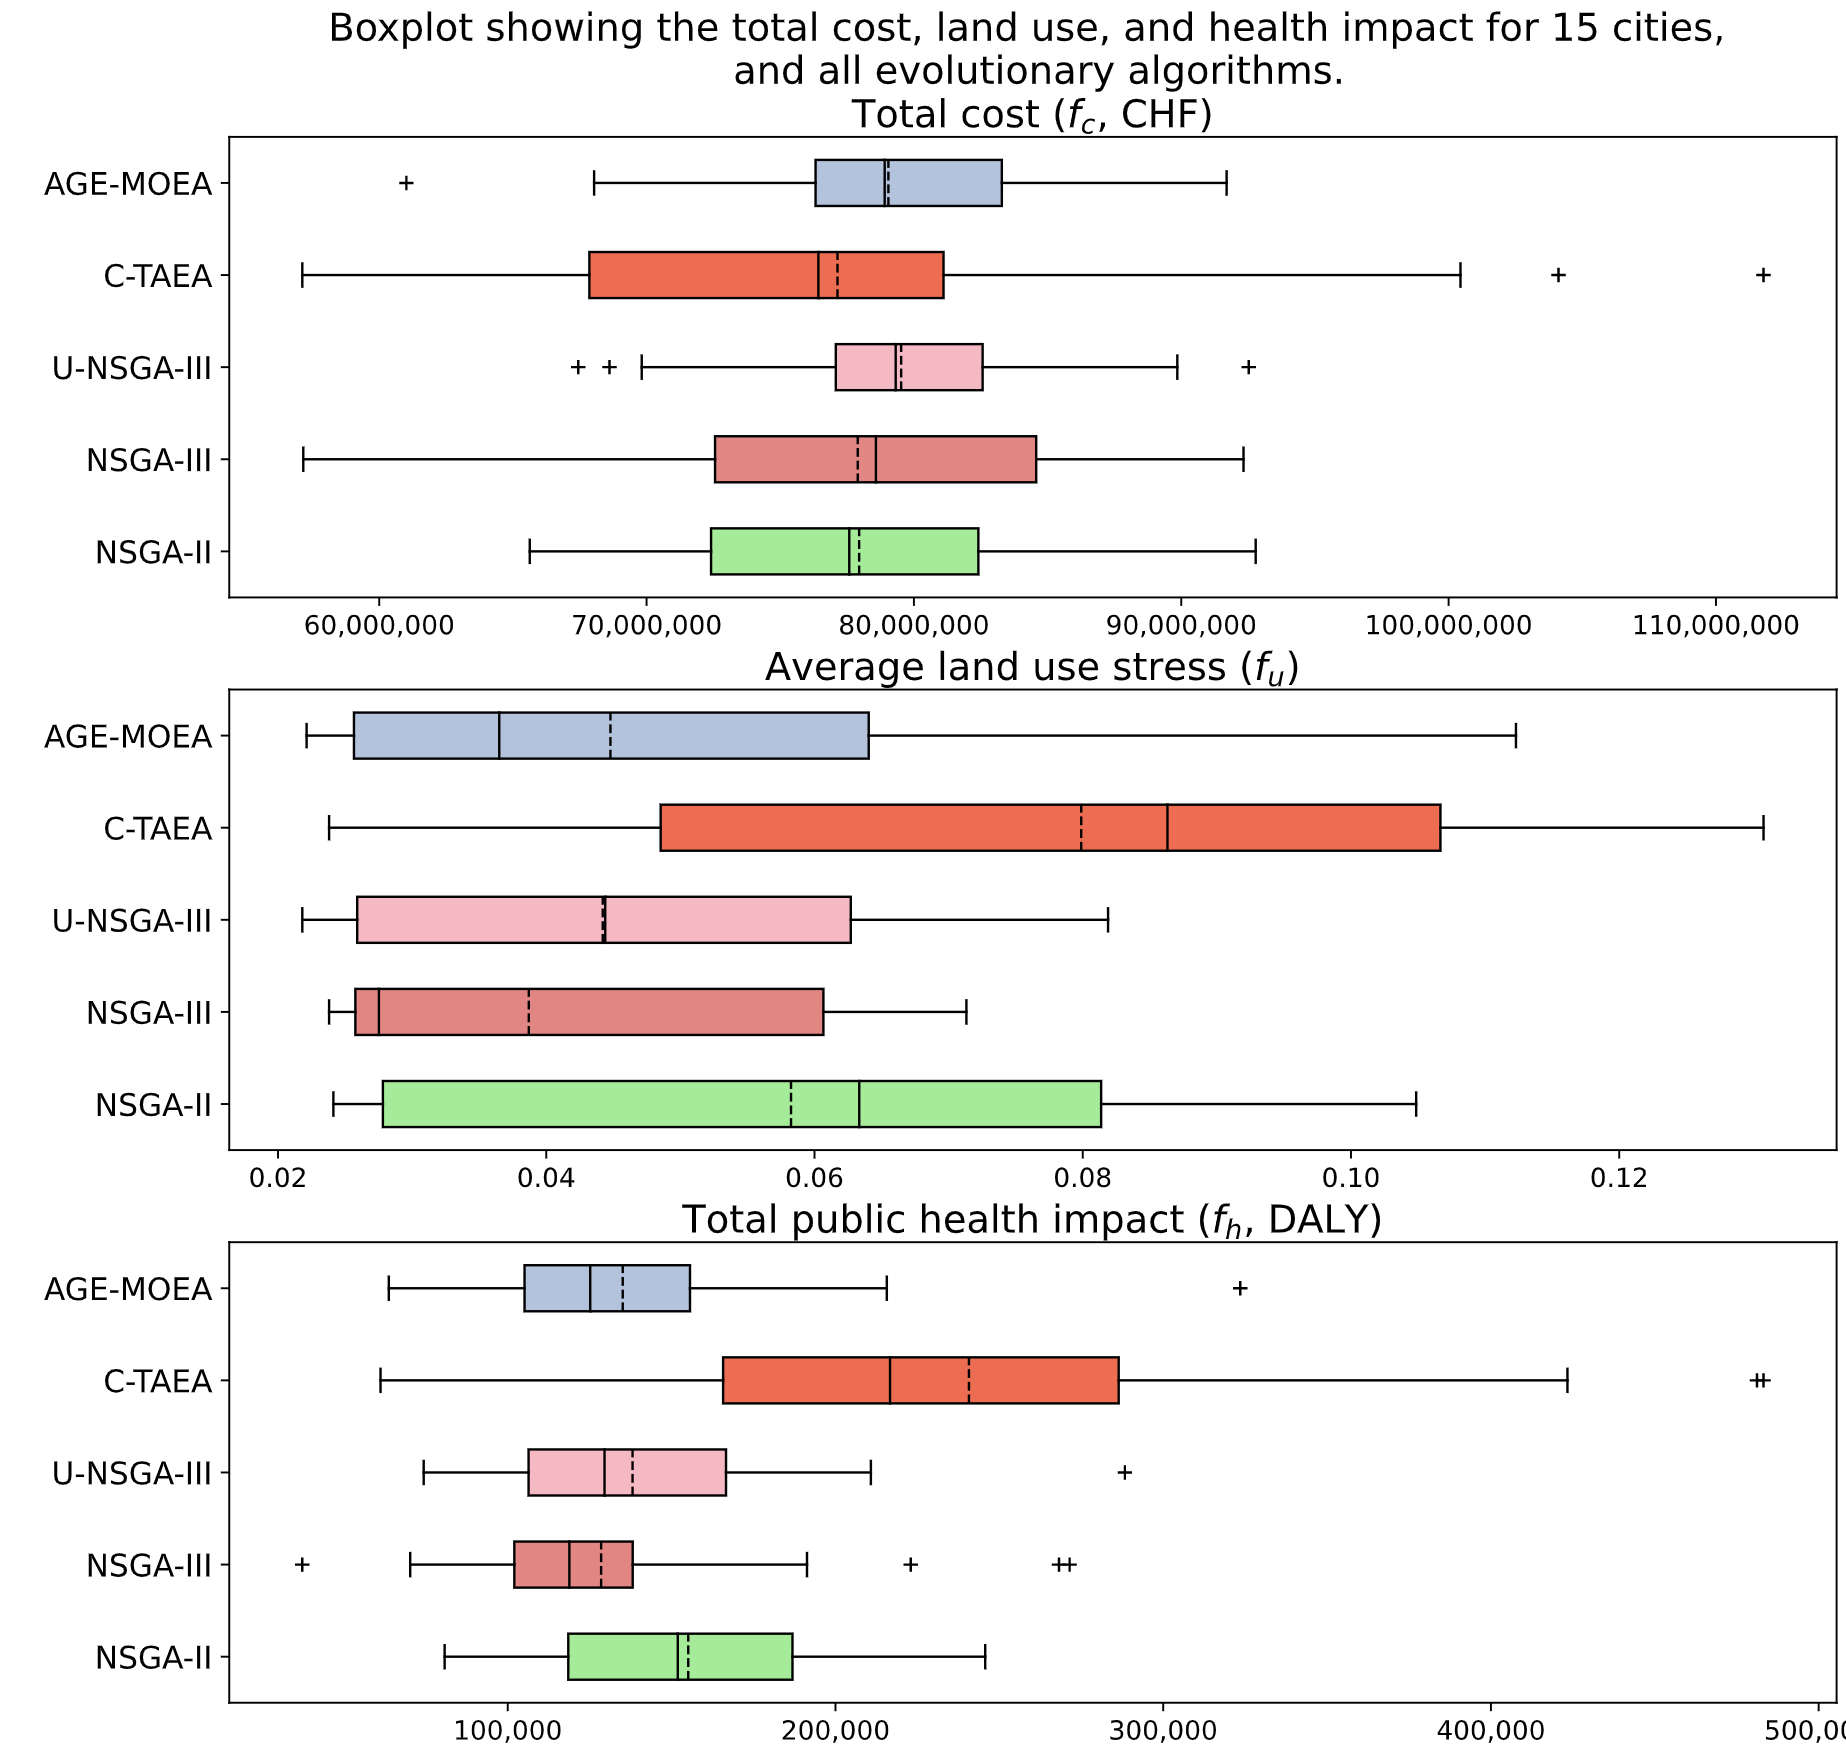
\includegraphics[width=1\textwidth]{/results/boxplots/boxplot_15_cities.png}
    \caption{Boxplot for 15 cities.}
    \label{fig:15_cities}
\end{subfigure}
\hfill
\begin{subfigure}{0.4\paperwidth}
    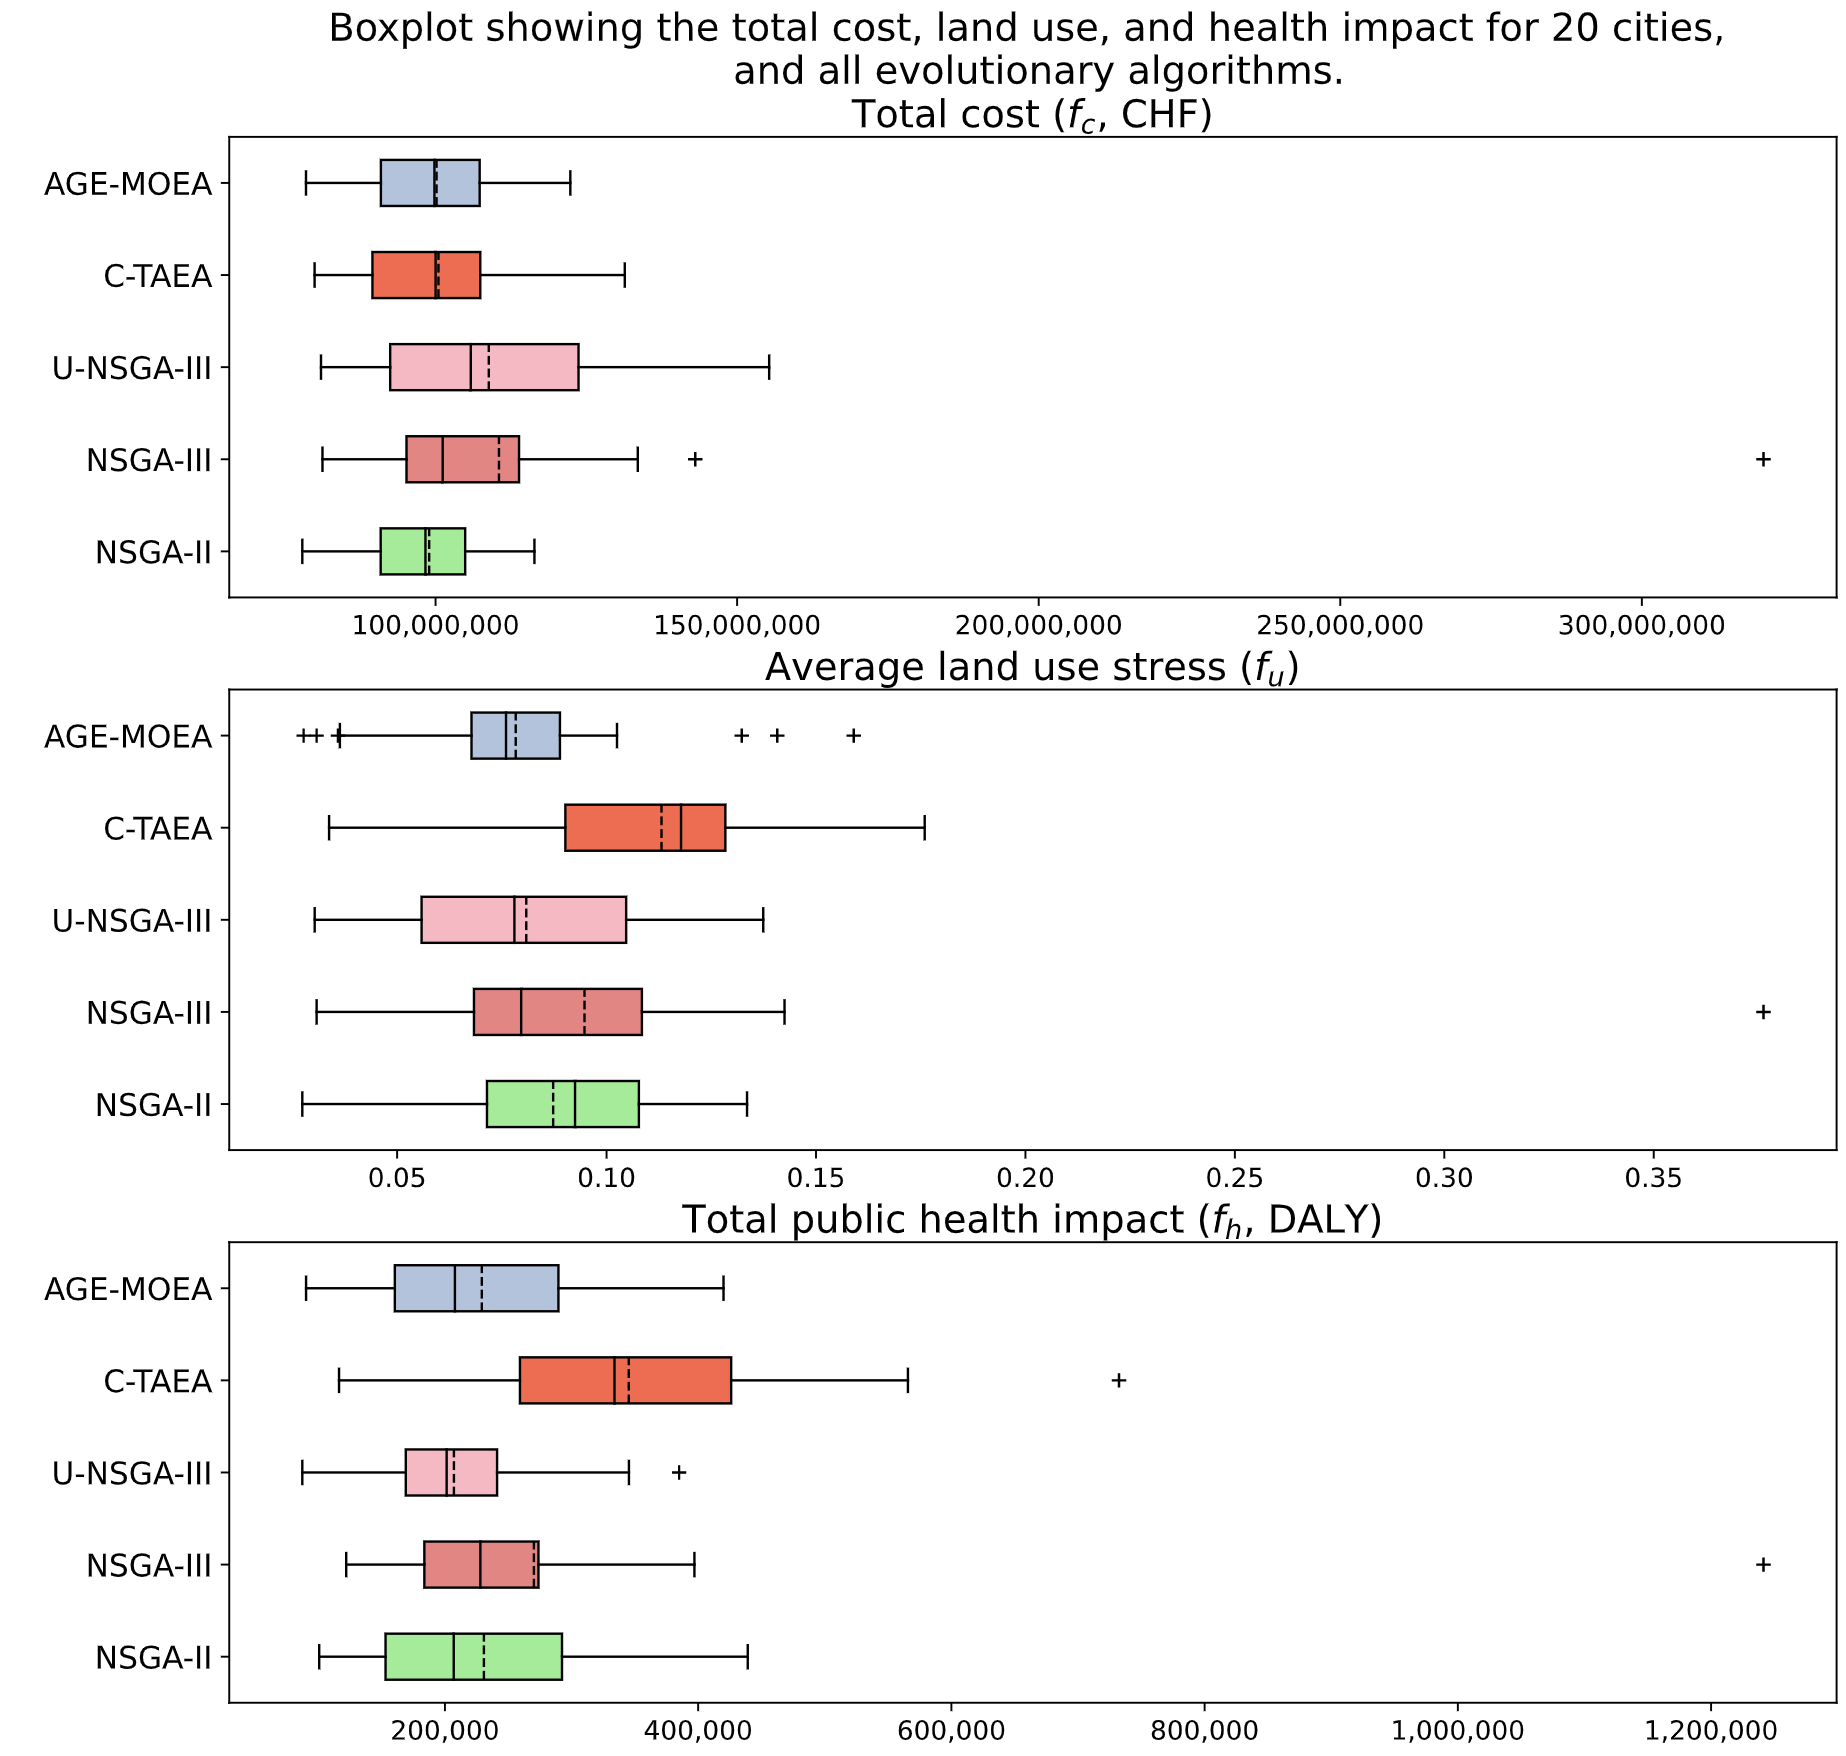
\includegraphics[width=1\textwidth]{/results/boxplots/boxplot_20_cities.png}
    \caption{Boxplot for 20 cities.}
    \label{fig:20_cities}
\end{subfigure}}
\hfill
\noindent\makebox[\textwidth]{
\begin{subfigure}{0.4\paperwidth}
    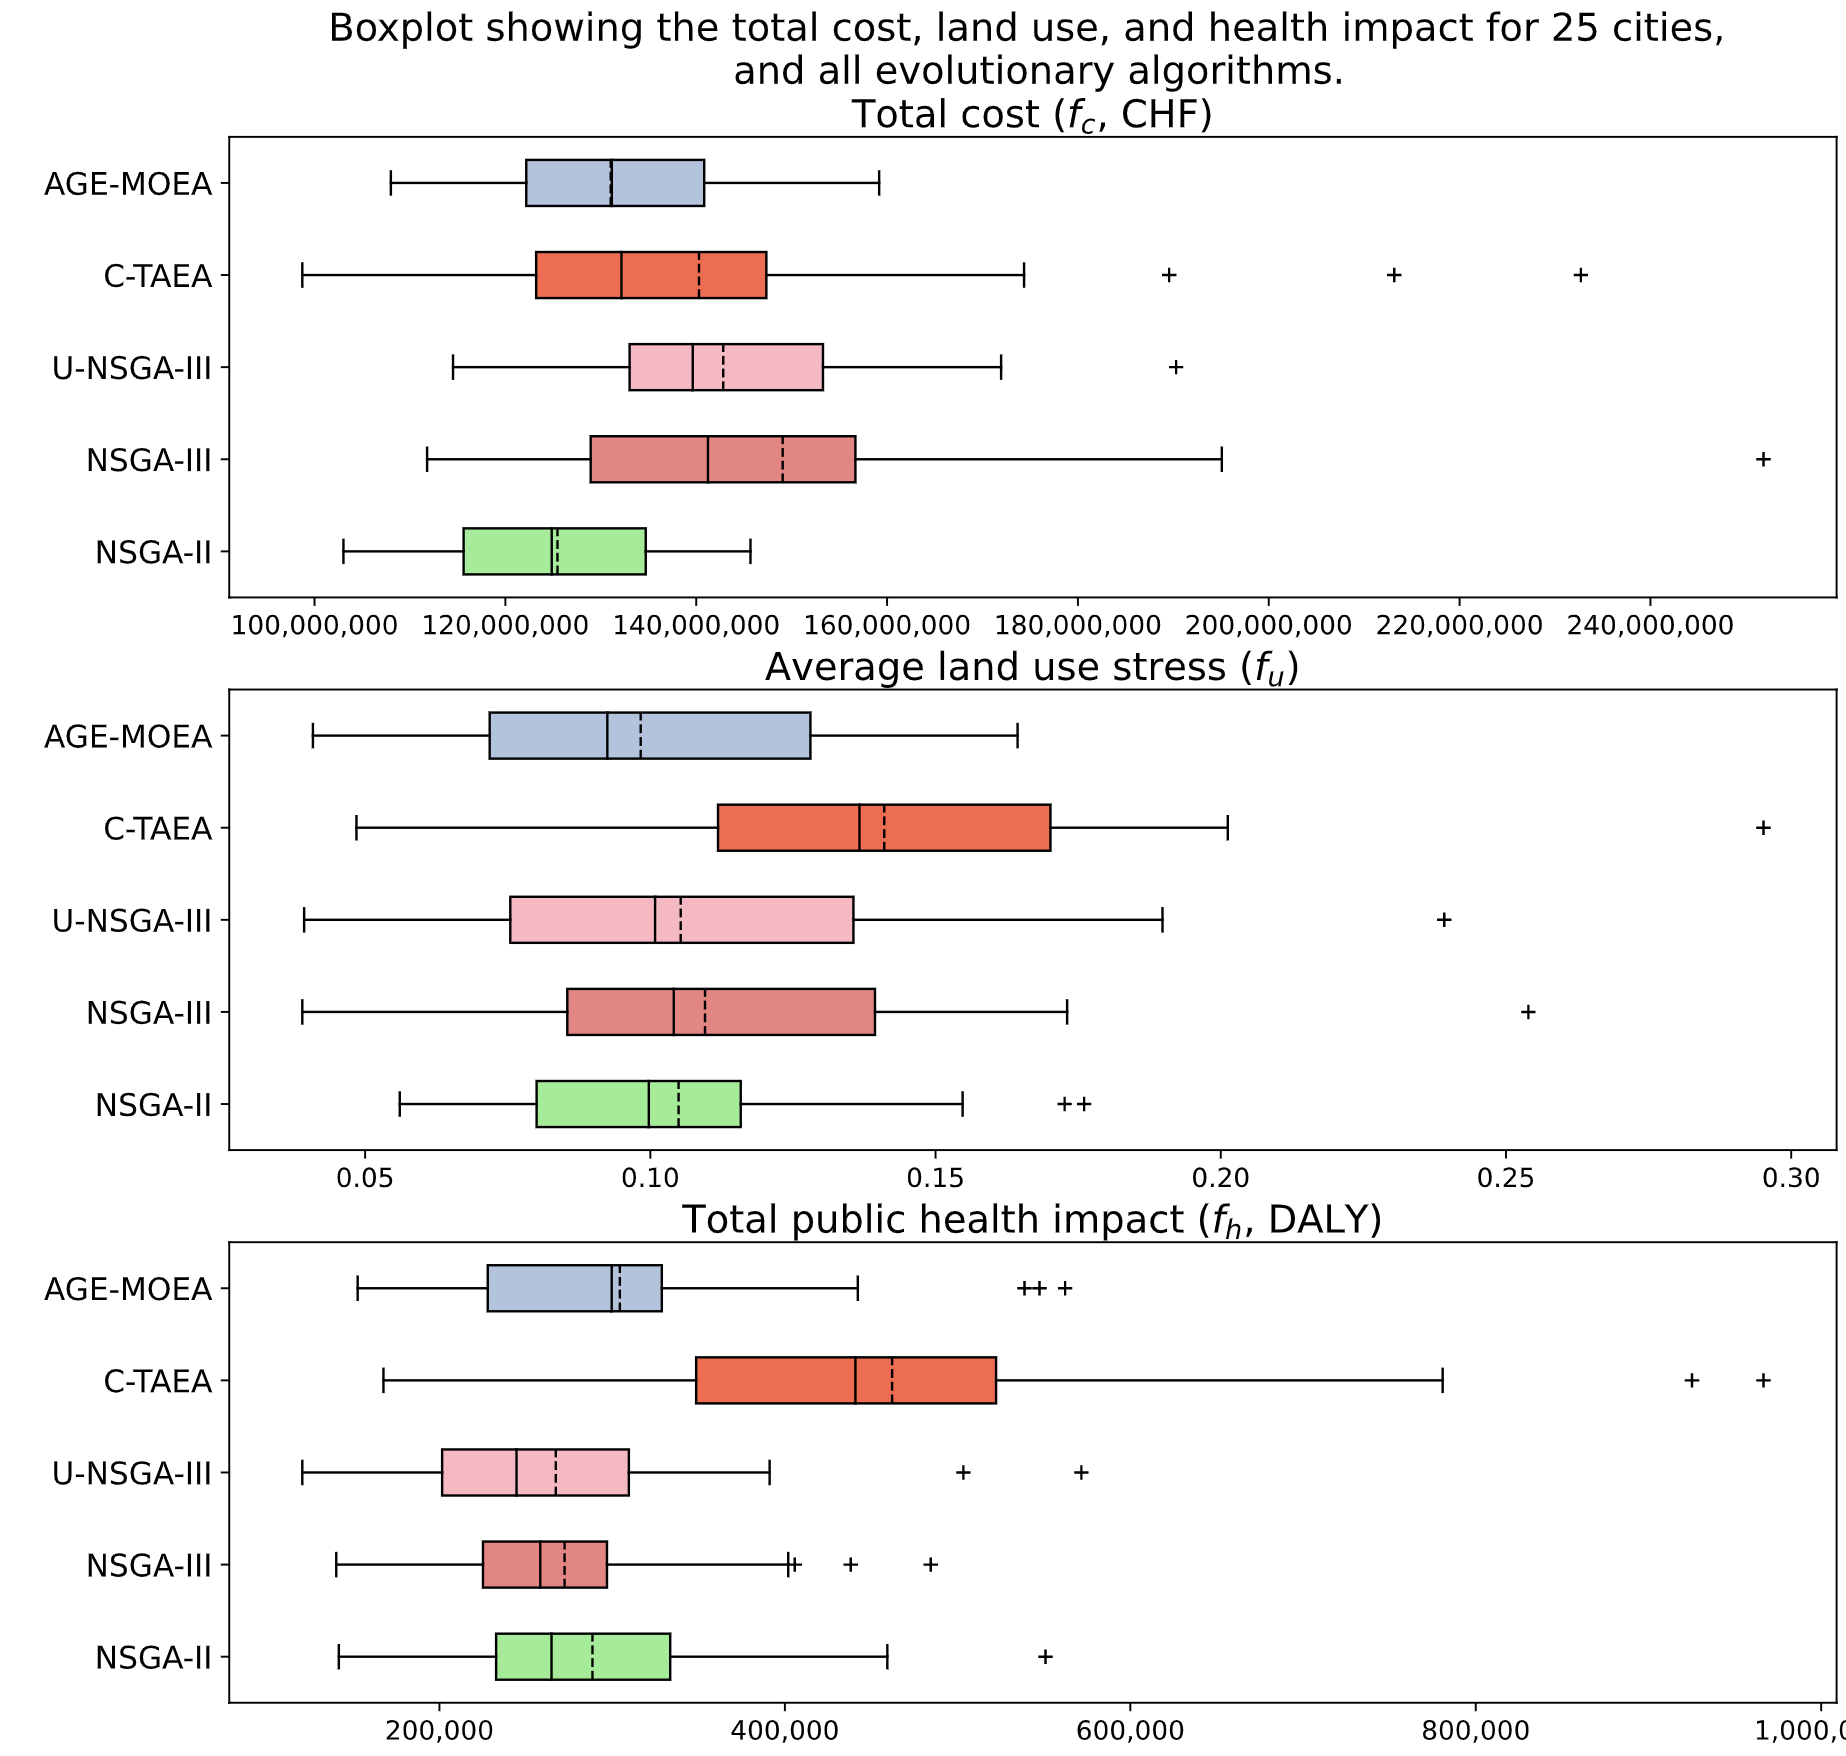
\includegraphics[width=1\textwidth]{/results/boxplots/boxplot_25_cities.png}
    \caption{Boxplot for 25 cities.}
    \label{fig:25_cities}
\end{subfigure}
\hfill
\begin{subfigure}{0.4\paperwidth}
    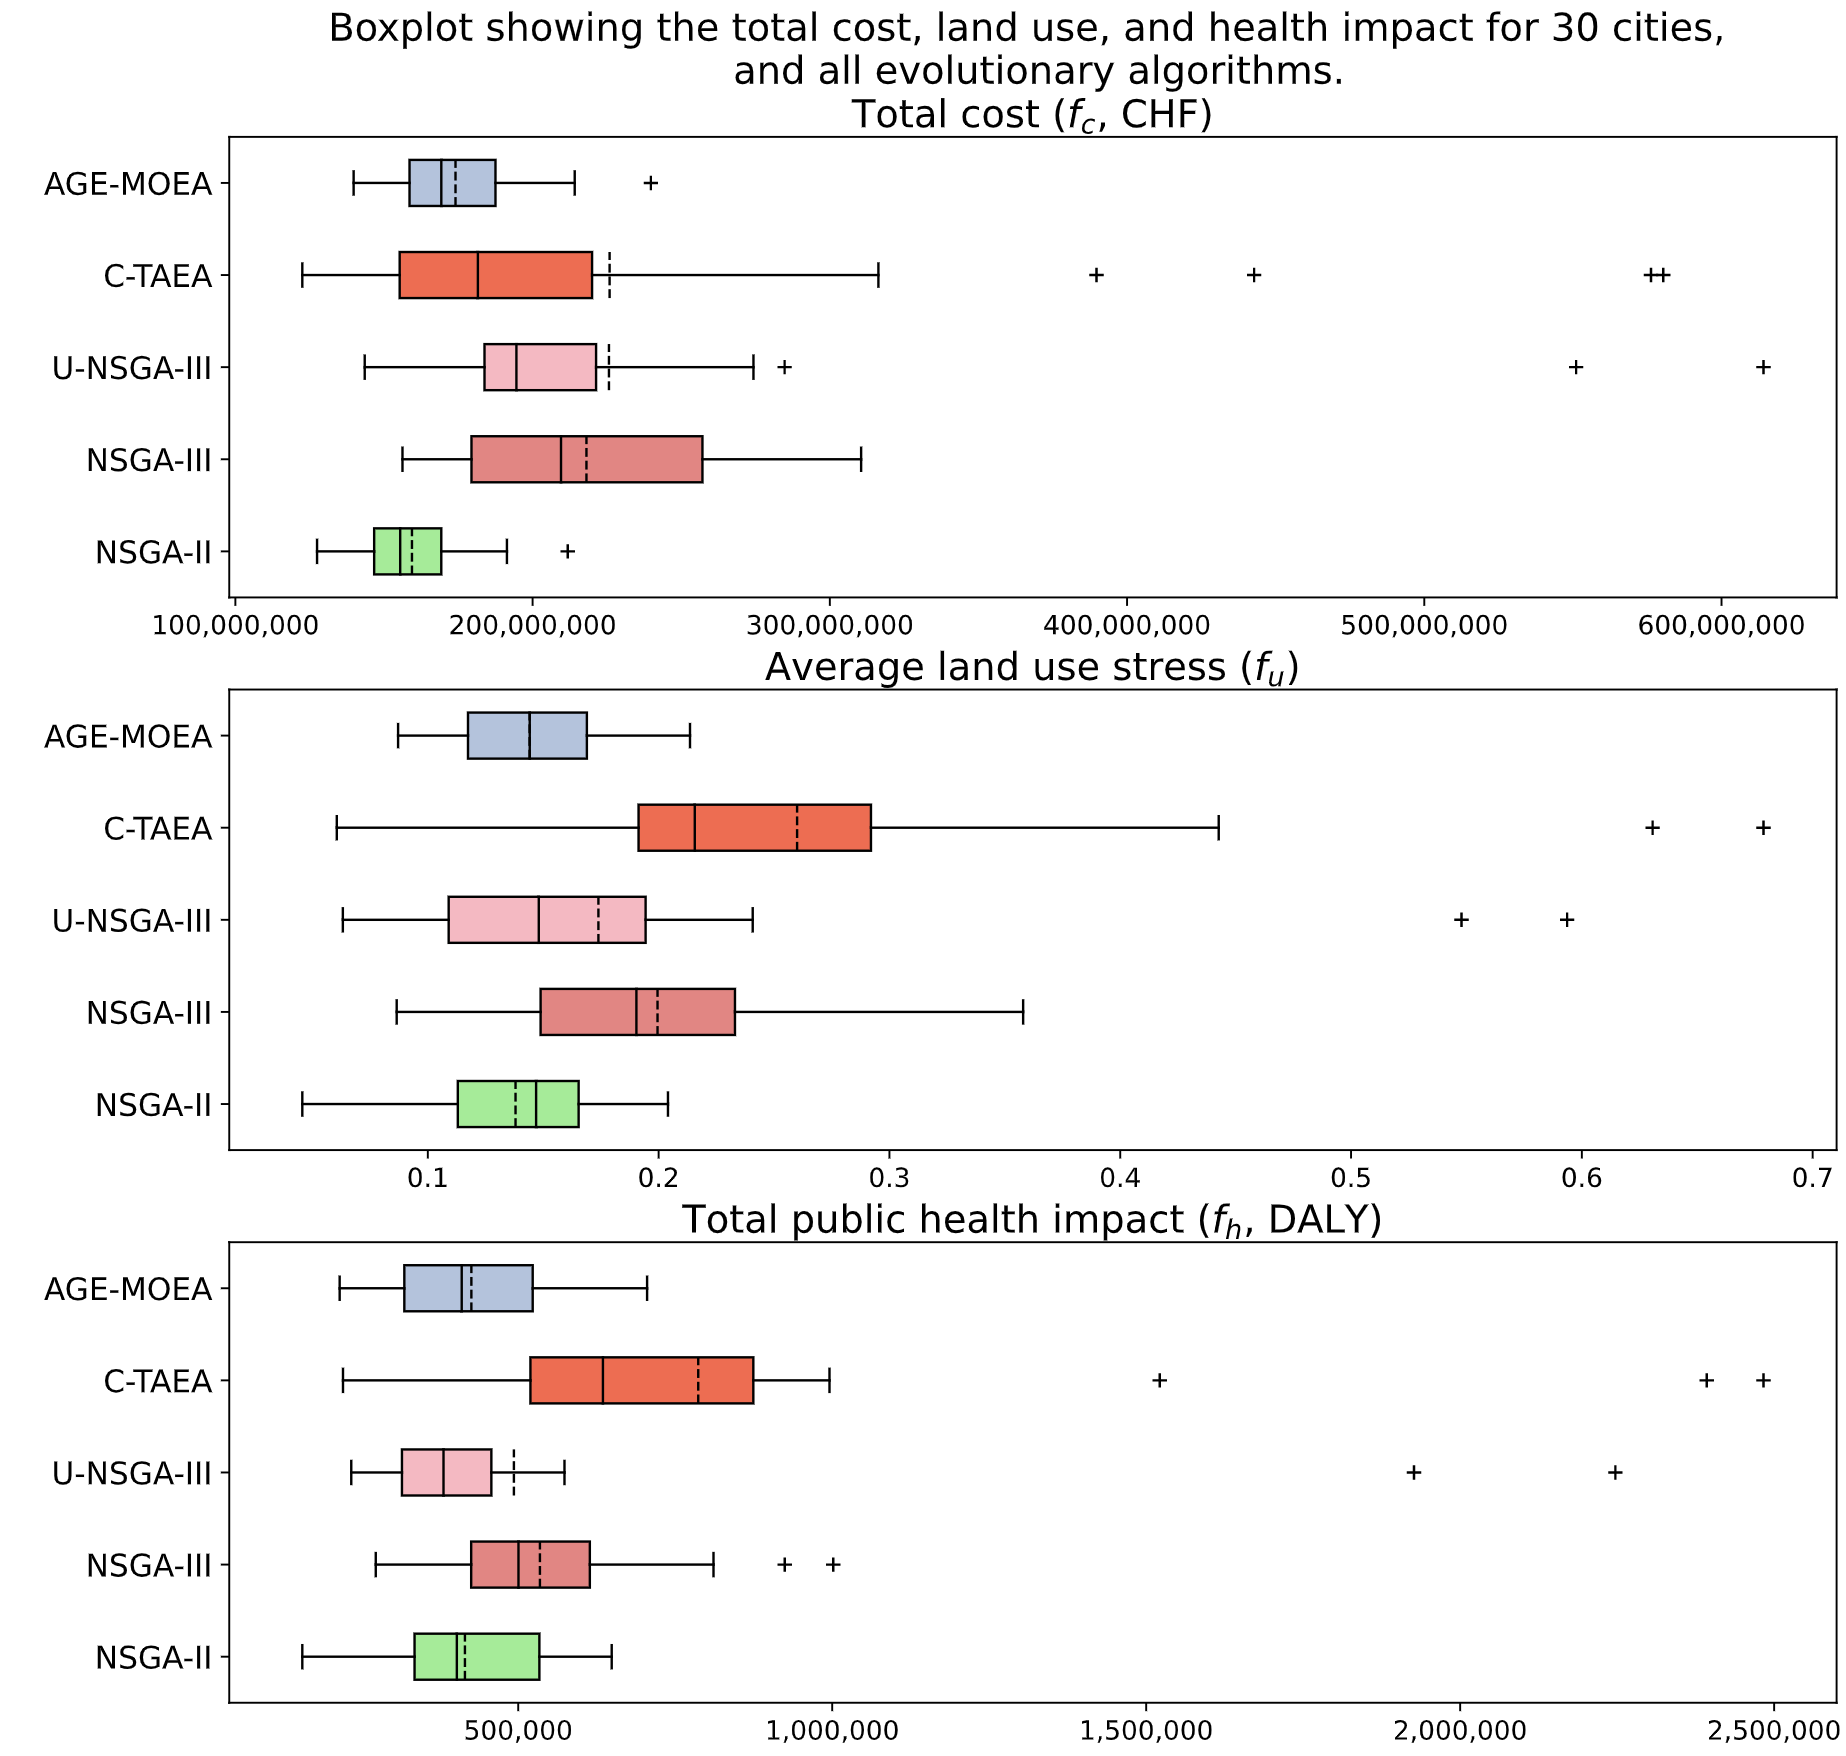
\includegraphics[width=1\textwidth]{/results/boxplots/boxplot_30_cities.png}
    \caption{Boxplot for 30 cities.}
    \label{fig:30_cities}
\end{subfigure}}
\hfill
\begin{subfigure}{0.4\paperwidth}
    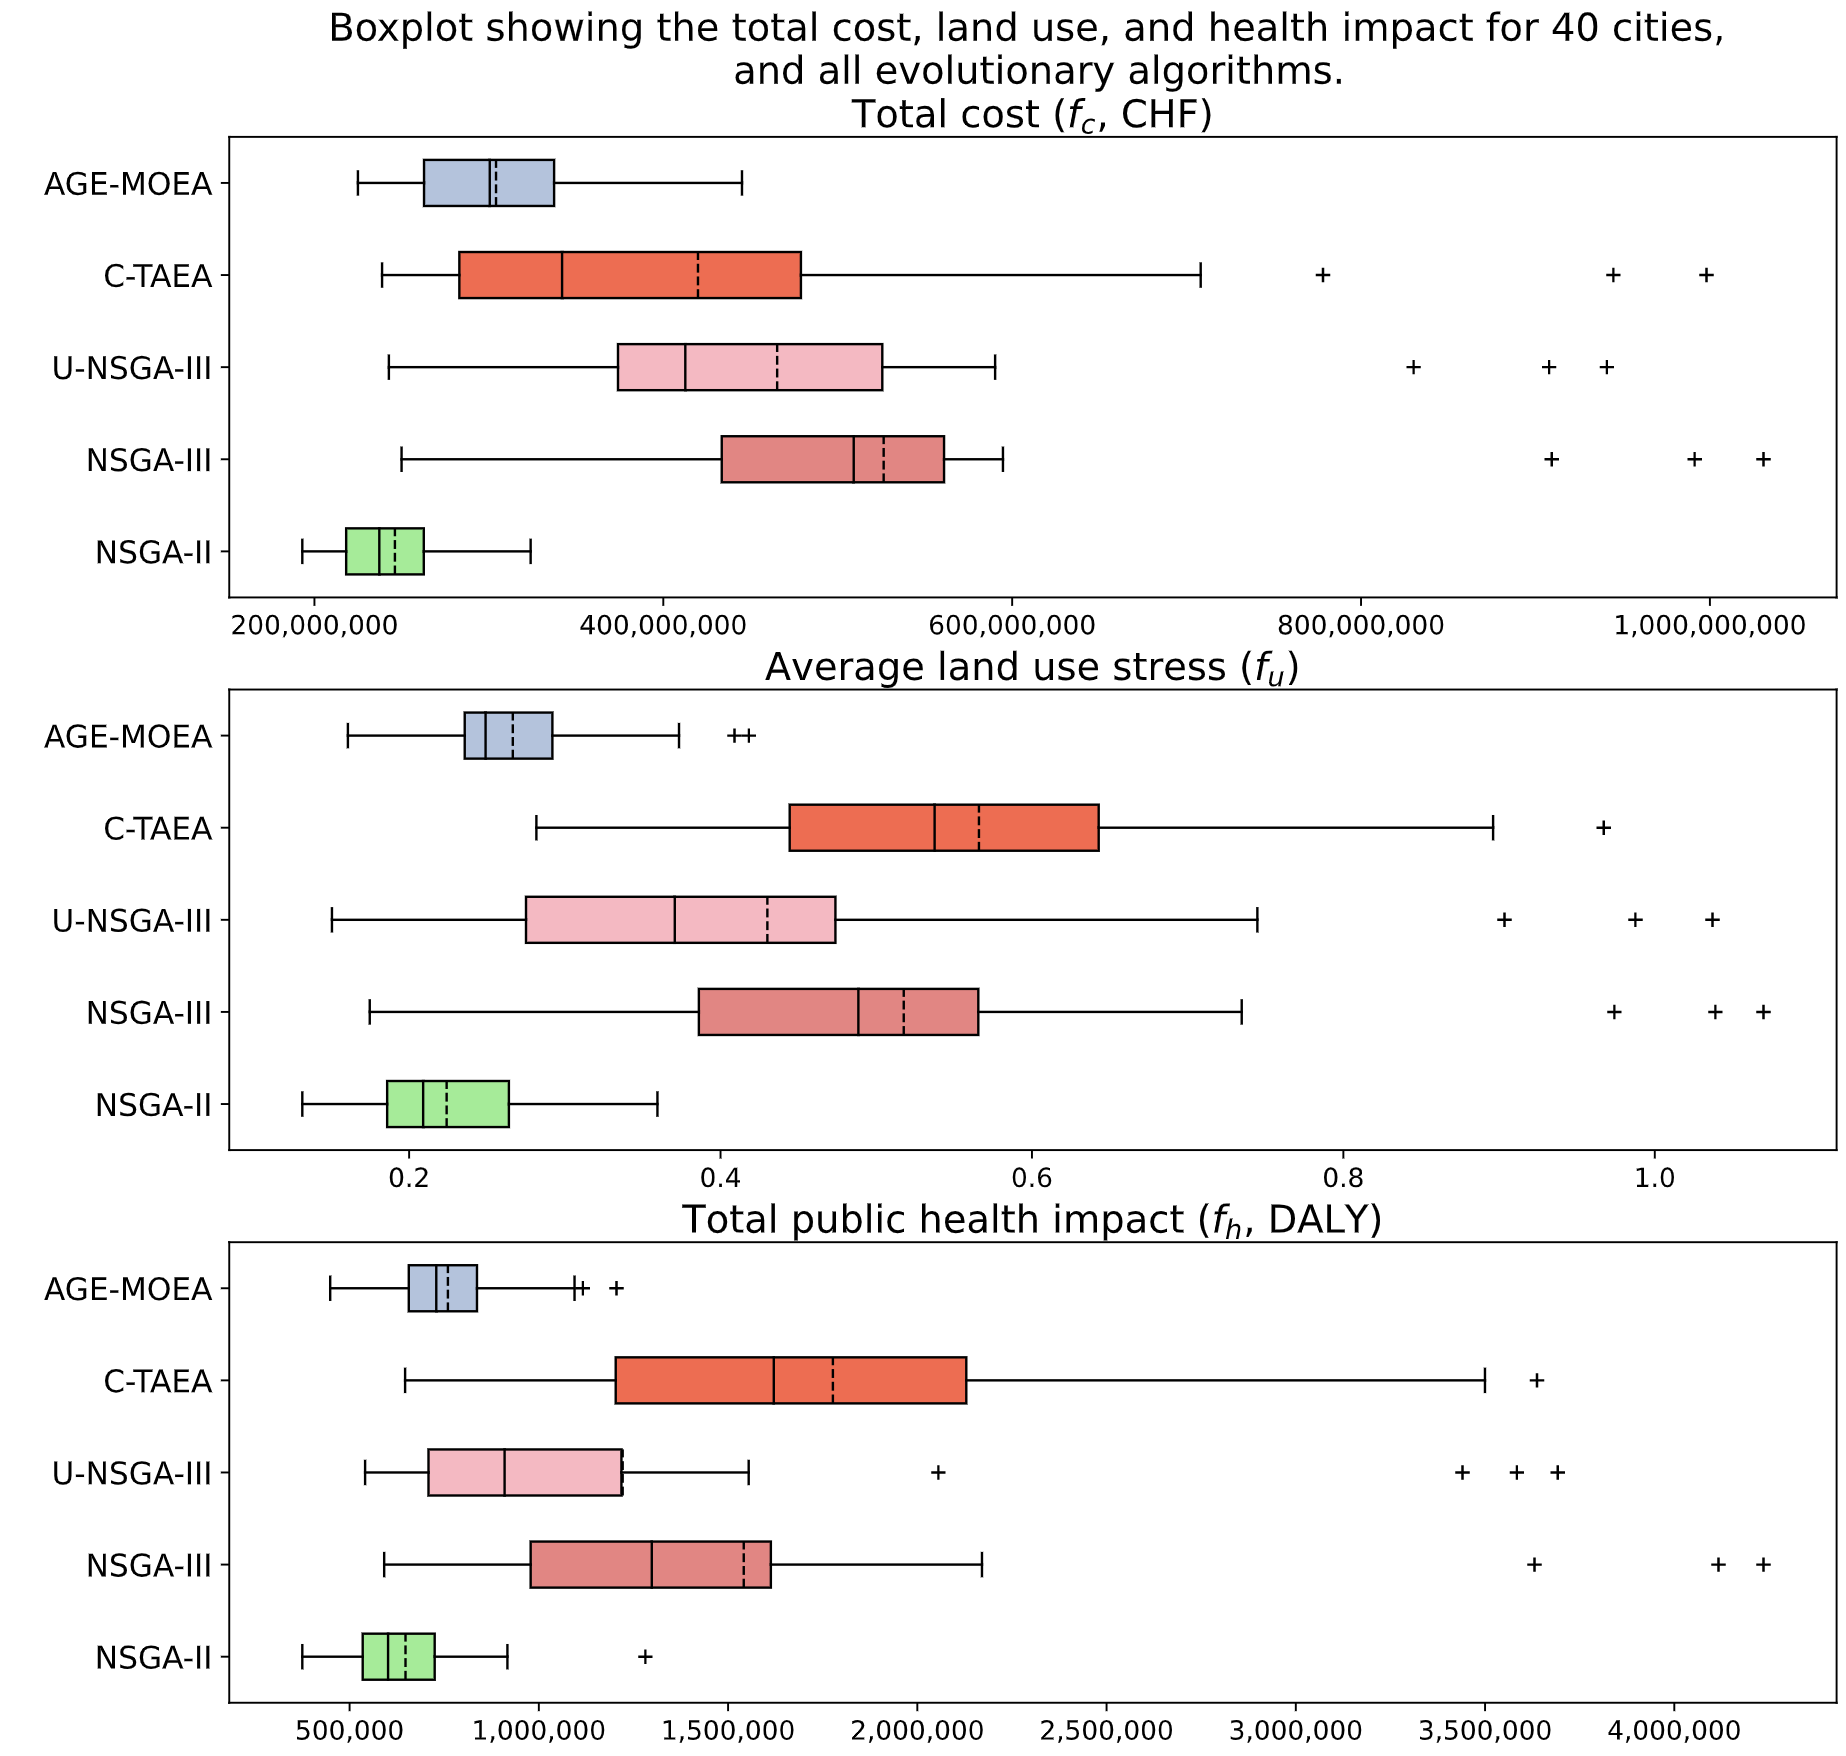
\includegraphics[width=1\textwidth]{/results/boxplots/boxplot_40_cities.png}
    \caption{Boxplot for 40 cities.}
    \label{fig:40_cities}
\end{subfigure}
\caption{Boxplots for large-scale problems showing the total cost, land usage stress and health impact for all evolutionary algorithms.}
\label{fig:boxplot_15_to_40}
\end{figure}

\clearpage
\section{Discussion}
Starting from the time claim, we conveyed in section \ref{sec:time_res} that the branch and cut algorithm takes much more time as the problem size increases. Due to the nature of the algorithm, it increases exponentially with the number of cities, while the evolutionary algorithms increase polynomially with the number of cities. Thus, we validate the claim of time.
\\\\
For the subsequent claim, we claimed that our method obtains reasonable solutions close to the branch and cut algorithm. The hypervolume results in section \ref{sec:hv_res} convey that most algorithms obtain close solutions based on the hypervolume. In some cities, the evolutionary algorithms even outperform the branch and cut. This outperformance could be due to the spread of solutions. When the evolutionary algorithms outperform the branch and cut algorithm, they find the lower minimum and maximum solutions than the branch and cut algorithm, which finds a smaller amount of spread-out solutions. However, the number of solutions does not necessarily correlate with the quality of the solutions. 
For example, NSGA-III and U-NSGA-III still find a good spread of solutions and a high hypervolume, even finding the highest hypervolume for nine cities in figure \ref{fig:hv_small} with only two solutions found in figure \ref{fig:sol_count_small} and still having a good spread of solutions for the cost and health impact in figure \ref{fig:9_cities}. 
\\\\
The final claim included the creation of trade-offs for the three objectives. The boxplots in figures \ref{fig:boxplot_2_to_5}, \ref{fig:boxplot_6_to_10}, and \ref{fig:boxplot_15_to_40}, all show a trade-off for each algorithm with them being better in two of the objectives however finding worse solutions for one objective. The branch and cut approach also shows this feature in some figures such as figure \ref{fig:2_cities} or \ref{fig:4_cities}, however usually finding a very low trade-off amount across the objectives such as in figures \ref{fig:3_cities} or \ref{fig:5_cities}. As the problem size gets larger, NSGA-II still finds trade-offs between solutions. C-TAEA finds the most trade-offs for large-scale solutions with an immense spread of solutions in \ref{fig:15_cities}, finding low costs and land usage while finding a moderately low health impact. Thus, we have validated that the evolutionary algorithm finds better trade-offs between the three objectives than the branch and cut algorithm.
\section{Conclusion}
For this chapter, we illustrated the observations of the empirical evidence in order to find differences between the proposed evolutionary algorithm method and the branch and cut approach. Furthermore, we also displayed the evolutionary algorithm results finding feasible solutions for large-scale problems. We convey that the claims established throughout this Thesis were validated, including the time taken, quality, and diversity of the solutions. 
\clearpage
\chapter[Conclusion]{Conclusion}
In conclusion, we presented an extension to the MILP model proposed by \cite{olapiriyakul_multiobjective_2019} using evolutionary multi-objective algorithms to allow for large-scale graphs and a Pareto front of diverse solutions. In addition, we have validated the claims regarding the time taken, the quality of solutions, and the diversity of the solutions by using statistical inferences. Furthermore, we adapted existing crossover and mutation operators for the evolutionary algorithms to solve the MILP problem with feasible reasonable solutions in polynomial time.
\\\\
The limitations of this approach are that as the problem size increases to huge problems, the evolutionary algorithm takes longer to find feasible solutions and sometimes converges to infeasible solutions, not finding them at all.
However, our method advances research in sustainable waste management for large-scale problems, as it consistently provides better solutions than previous approaches. 
\\\\
Future work for this problem could include a deeper look into the sorting facilities as well as into sorting the waste instead of fully forwarding it to the incinerator or landfill facilities. Additionally, one should consider new algorithms that focus on finding better feasible solutions for large-scale problems faster.

\backmatter

% \chapter{Glossary} %optional

% \bibliographystyle{alpha}
% \bibliographystyle{dcu}
\bibliographystyle{plainnat}
\bibliography{biblio}

%\cleardoublepage
% \theindex %optional, use only if you have an index, must use
	  %\makeindex in the preamble

\end{document}
